\RequirePackage{amsmath} 

\documentclass[graybox,envcountsect]{svmono}

\usepackage[T1]{fontenc}
\usepackage[utf8]{inputenc}

\usepackage{amsmath}
\usepackage[notref,notcite]{showkeys}
\usepackage{float}
\usepackage{amssymb}
\usepackage{amstext}
\usepackage{mathtools}
\usepackage{xcolor} 
\usepackage{centernot}
\usepackage{listings}
\usepackage{multicol}
\usepackage{mathptmx}
%\usepackage{newtxtext,newtxmath}
%\usepackage{txfonts}
\usepackage{datetime}
\usepackage{tikz-cd}

\usepackage{helvet}
\usepackage{courier}
\usepackage{type1cm}         
\usepackage{makeidx}        
\usepackage{graphicx}        
\usepackage{multicol}        
\usepackage[all]{xy}
\usepackage{hyperref} 
%\usepackage{tikz-cd}

\usepackage[small,bf]{caption}

\usepackage{tikz}
\usetikzlibrary{braids}
	
\usepackage[bottom]{footmisc}

% for QED
\let\proof\relax\let\endproof\relax
\usepackage{amsthm}

\overfullrule=1mm

%%% for Spanish
% \def\abstractname{Resumen}%
% \def\ackname{Agradecimientos}%
% \def\andname{y}%
% \def\bibname{Referencias}%
% \def\lastandname{, y}%
% \def\appendixname{Apéndice}%
% \def\chaptername{Capítulo}%
% \def\claimname{Afirmación}%
% \def\conjecturename{Conjetura}%
% \def\contentsname{Contenidos}%
% \def\corollaryname{Corolario}%
% \def\definitionname{Definici\'on}%
% \def\emailname{e-mail}%
% \def\examplename{Ejemplo}%
% \def\examplesname{Ejemplos}%
% \def\exercisename{Ejercicio}%
\def\figurename{Figure}%
% \def\forewordname{Foreword}%
% \def\keywordname{{\bf Palabras clave:}}%
% \def\indexname{Índice}%
% \def\lemmaname{Lema}%
% \def\listfigurename{Figuras}%
% \def\listtablename{Tablas}%
% \def\notename{Nota}%
% \def\partname{Parte}%
% \def\prefacename{Prefacio}%
% \def\problemname{Problema}%
% \def\proofname{Demostración}%
% \def\propertyname{Propiedad}%
% \def\propositionname{Proposici\'on}%
% \def\questionname{Pregunta}%
% \def\refname{Referencias}%
% \def\remarkname{Observación}%
% \def\seename{see}%
% \def\solutionname{Solución}%
% \def\tablename{Tabla}%
% \def\theoremname{Teorema}
\def\notationname{Notation}
\def\stepsname{Algorithm}
% \def\conventionname{Convención}

% change numbers 
\let\remark\relax
\let\theorem\relax
\let\lemma\relax
\let\definition\relax
\let\proposition\relax
\let\corollary\relax
\let\exercise\relax
\let\example\relax
\let\conjecture\relax
\spnewtheorem{theorem}{\theoremname}[section]{\bfseries}{\itshape}
\renewcommand\thetheorem{\thesection.\arabic{theorem}}
\spnewtheorem{lemma}[theorem]{\lemmaname}{\bfseries}{\itshape}
\spnewtheorem{definition}[theorem]{\definitionname}{\bfseries}{\upshape}
\spnewtheorem{proposition}[theorem]{\propositionname}{\bfseries}{\itshape}
\spnewtheorem{corollary}[theorem]{\corollaryname}{\bfseries}{\itshape}
\spnewtheorem{exercise}[theorem]{\exercisename}{\bfseries}{\upshape}
\spnewtheorem{example}[theorem]{\examplename}{\bfseries}{\upshape}
\spnewtheorem{examples}[theorem]{\examplesname}{\bfseries}{\upshape}
\spnewtheorem{remark}[theorem]{\remarkname}{}{\upshape}
\spnewtheorem{conjecture}[theorem]{\conjecturename}{\bfseries}{\upshape}
\spnewtheorem{notation}[theorem]{\notationname}{\bfseries}{\upshape}
\spnewtheorem{steps}[theorem]{\stepsname}{\bfseries}{\upshape}
\spnewtheorem{convention}[theorem]{\conventionname}{\bfseries}{\upshape}

% para enumerar
\renewcommand{\labelenumi}{\textbf{\arabic{enumi})}}

\makeindex             

\renewcommand{\I}{\operatorname{I}}
\newcommand{\II}{\operatorname{II}}

\newcommand{\GAP}{\textsf{GAP}}
\newcommand{\FK}{\mathcal{E}}
\newcommand{\ad}[1]{\operatorname{ad}\,#1}

\newcommand{\N}{\mathbb{N}}
\newcommand{\Q}{\mathbb{Q}}
\newcommand{\Z}{\mathbb{Z}}
\newcommand{\F}{\mathbb{F}}
\newcommand{\R}{\mathbb{R}}
\newcommand{\C}{\mathbb{C}}
\renewcommand{\H}{\mathbb{H}}
\newcommand{\A}{\mathbb{A}}
\newcommand{\K}{\mathbb{K}}
\newcommand{\T}{\mathbb{T}}
\renewcommand{\D}{\mathbb{D}}
\newcommand{\B}{\mathbb{B}}
\newcommand{\Fun}{\operatorname{Fun}}
\newcommand{\mpl}{\operatorname{mpl}}
\newcommand{\cL}{\mathcal{L}}
\newcommand{\cE}{\mathcal{E}}
\newcommand{\cH}{\mathcal{H}}

\newcommand{\GF}{\mathsf{GF}}
\newcommand{\MAX}{\operatorname{MAX}}
\newcommand{\MIN}{\operatorname{MIN}}
\newcommand{\cf}{\operatorname{cf}}
\newcommand{\cl}{\operatorname{cl}}
\newcommand{\cd}{\operatorname{cd}}
\newcommand{\bL}{\mathbf{L}}
\newcommand{\bP}{\mathbf{P}}

\newcommand{\Nil}{\operatorname{Nil}}
\newcommand{\rad}{\operatorname{rad}}
\newcommand{\rank}{\operatorname{rank}}

\newcommand{\Aff}{\mathrm{Aff}}
\newcommand{\Ann}{\operatorname{Ann}}
\newcommand{\Der}{\operatorname{Der}}
\newcommand{\Core}{\operatorname{Core}}
\newcommand{\Soc}{\operatorname{Soc}}
\newcommand{\Fix}{\operatorname{Fix}}
\newcommand{\Rad}{\mathrm{rad}}
\newcommand{\Inn}{\mathrm{Inn}}
\newcommand{\dist}{\mathrm{dist}}
\newcommand{\Out}{\mathrm{Out}}
\newcommand{\Ext}{\mathrm{Ext}}
\newcommand{\Img}{\mathrm{im}}
\newcommand{\Hol}{\operatorname{Hol}}
\newcommand{\Hom}{\operatorname{Hom}}
\newcommand{\Alg}{\operatorname{Alg}}
\newcommand{\Bil}{\operatorname{Bil}}
\newcommand{\op}{\operatorname{op}}
\newcommand{\gr}{\operatorname{gr}}
\newcommand{\Syl}{\mathrm{Syl}}
\newcommand{\id}{\operatorname{id}}
\newcommand{\Aut}{\operatorname{Aut}}
\newcommand{\End}{\operatorname{End}}
\newcommand{\Irr}{\operatorname{Irr}}
\newcommand{\Alt}{\mathbb{A}}
\newcommand{\Sym}{\mathbb{S}}
\newcommand{\lcm}{\mathrm{mcm}}
\newcommand{\diag}{\operatorname{diag}}
\newcommand{\spec}{\operatorname{Spec}}
\newcommand{\supp}{\operatorname{supp}}
\newcommand{\trace}{\operatorname{traza}}
\newcommand{\sgn}{\operatorname{signo}}

\newcommand{\inner}{\operatorname{inn}}
\newcommand{\ext}{\operatorname{ext}}
\newcommand{\im}{\operatorname{im}}
\newcommand{\Ret}{\operatorname{Ret}}

\newcommand{\GL}{\mathbf{GL}}
\newcommand{\SL}{\mathbf{SL}}
\newcommand{\PSL}{\mathbf{PSL}}
\newcommand{\PGL}{\mathbf{PGL}}

\newcommand{\legendre}[2]{\left(\frac{#1}{#2}\right)}

%\newcommand{\char}{\operatorname{char}}

% multiset
\def\multiset#1#2{\ensuremath{\left(\kern-.3em\left(\genfrac{}{}{0pt}{}{#1}{#2}\right)\kern-.3em\right)}}


% column vector
\newcount\colveccount
\newcommand*\colvec[1]{
\global\colveccount#1
\begin{pmatrix}
	\colvecnext
	}
	\def\colvecnext#1{
	#1
	\global\advance\colveccount-1
	\ifnum\colveccount>0
	\\
	\expandafter\colvecnext
	\else
\end{pmatrix}
\fi
}

% numero como secciones
\renewcommand{\thesection}{\arabic{chapter}} 


% To remove Springer from the title page
\usepackage{etoolbox}
\makeatletter
\patchcmd{\@maketitle}{{\Large Springer\par}}{}{}{}
\makeatother

\begin{document}

\lstset{language=GAP,
  showstringspaces=false,
  xleftmargin=0.6cm,
  xrightmargin=0.6cm,
  basicstyle=\small\ttfamily,
  frame=single,
  framerule=0pt,
}


\author{Leandro Vendramin}
\title{Groups, radical rings and the Yang--Baxter equation}
\subtitle{A combinatorial approach to solutions}
\maketitle

\frontmatter

\begin{dedication}
A Dino
\end{dedication}





%\include{foreword}

The Yang--Baxter equation (YBE) arose from Yang's work on statistic mechanics. In 1967 Yang tried to find the eigenfunctions of a one-dimensional fermion gas with delta function inteaction. This was
a rather difficult problem. He solved it and showed that a crucual identity in the intermediate steps was a matrix equation
\[
A(u)B(u+v)A(v)=B(v)A(u+v)B(u).
\]
Later, Baxter, in his solution of another problem in physics, the 8-vertex model again used the YBE. 
In 1980 Faddeev coined the term "Yang-Baxter Equation". A number of exciting developmenents in 
physics and mathematics have led to the conclusion that the YBE is a fundamental mathematical structure with connections to various subfields of mathematics such as 
knot theory, braid theory, operator theory, Hopf algebras, quantum groups, 3-manifolds, the monondromy of differential equations...

\begin{quote}
    I got the feeling that the YBE is the next pervasive algebraic equation after the Jacobi identity.
\end{quote}

\framebox{Compiled: \today,~\currenttime.}

\medskip
In Chapter~\ref{YB} basic definitions and examples of solutions introduced. 
The main result of the chapter is Theorem~\ref{thm:LYZ}, 
where the deep relationship between
solutions and group actions is studied. 

The first part of Chapter~\ref{radical} provides an introduction to the theory of radical rings.
The material presented is pretty standard. 
After recalling basic definitions and stating basic properties, the theory of the Jacobson
radical is explored. The second part of the chapter is devoted to involutive solutions. One of the
main results of this chapter is Rump's theorem, which states that radical rings produce solutions. 
In this
chapter we also introduce cycle sets, which are structures that turns out to be equivalent
to involutive solutions. 

In Chapter~\ref{braces} we introduce the theory of braces. One of the main results of this 
chapter is Theorem~\ref{thm:}, which proves that braces produce arbitrary solutions. We introduce
skew cycle sets and prove in Theorem... that skew cycle sets and arbitrary solutions are equivalent. 

In Chapter~\ref{cocycles} we complements and 1-cocycles. 
In Theorem... 
Sysak's theorem states that...

The first part of Chapter~\ref{nilpotent} is devoted to the general theory of nilpotent groups. 
The second part is devoted to the Frattini subgroup and some of its applications
The fourth part is about a sort of Frattini subgroup in the context of braces. 


Chapter~\ref{solvable} is about solvable groups. The basic theory of solvable groups is presented in the first section. We
prove Wielandt's three subgroups theorem and Hall's theorem. 

Chapter~\ref{factorization} is about factorization of groups and braces. First
we prove It\^o's theorem in the case of groups: Every group that admits a factorization through two 
abelian subgroups is meta-abelian. The second section is about solvability of structure groups
of involutive solutions and related concepts. 

In Chapter~\ref{structure_brace} we prove one of the main results of the book. The existence of a universal brace
that somewhat classifies solutions. 




Thanks: Jingpeng Shen

\medskip
Versión compilada el \today~a las~\currenttime.

\begin{flushright}
Leandro Vendramin\\Buenos Aires, Argentina\par
\end{flushright}

%\include{acknow}

\tableofcontents

%\include{acronym}

\mainmatter

%\include{part}
\chapter{The Yang--Baxter equation}
\label{YB}

%\section*{A}

In \cite{MR1183474}, Drinfeld briefly discuss set-theoretic solutions to the Yang--Baxter equation. 
He observed that
it makes sense to consider the Yang--Baxter equation in the category of sets and that 
"maybe it would be interesting to study set-theoretical solutions". 

\begin{definition}
\index{Solution}
\index{Solution!finite}
A \emph{set-theoretic solution} to the Yang--Baxter equation (YBE) is a pair $(X,r)$, 
where $X$ is a set and $r\colon X\times X\to X\times X$ is a bijective map that satisfies 
\[
(r\times\id)(\id\times r)(r\times\id)=
(\id\times r)(r\times\id)(\id\times r),
\]
where, if $r(x,y)=(\sigma_x(y),\tau_y(x))$, then 
\begin{align*}
& r\times\id\colon X\times X\times X\to X\times X\times X, &&(r\times\id)(x,y,z)=(\sigma_x(y),\tau_y(x),z),\\
& \id\times r\colon X\times X\times X\to X\times X\times X, &&(\id\times r)(x,y,z)=(x,\sigma_y(z),\tau_z(y)).
\end{align*}
The solution $(X,r)$ is said to be \emph{finite} if $X$ is a finite set. 
\end{definition}

\begin{figure}
\centering
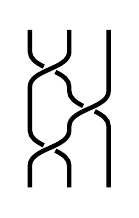
\begin{tikzpicture}
\pic[
  braid/.cd,
  number of strands=3,
  height=.5cm,
  width=.5cm,
  ultra thick,
  gap=0.1,
  name prefix=braid,
] {braid={a_{1}a_2a_1}};
\end{tikzpicture}
\hspace{1cm}
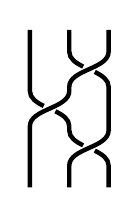
\begin{tikzpicture}
\pic[
  braid/.cd,
  number of strands=3,
  height=.5cm,
  width=.5cm,
  ultra thick,
  gap=0.1,
  name prefix=braid,
] {braid={a_{2}a_1a_2}};
\end{tikzpicture}
\caption{The Yang--Baxter equation.}
\label{fig:braid}
\end{figure}

\index{Braid group}
For $n\geq2$, the \emph{braid group} $\B_n$ is defined as the group with generators $\sigma_1,\dots,\sigma_{n-1}$ and relations
\begin{align*}
    &\sigma_i\sigma_{i+1}\sigma_i=\sigma_{i+1}\sigma_i\sigma_{i+1} && \text{if }1\leq i\leq n-2,\\
    &\sigma_i\sigma_j=\sigma_j\sigma_i && \text{if }|i-j|\geq 1.
\end{align*}
Let $(X,r)$ be a set-theoretic solution to the YBE. Write $X^n=X\times\cdots\times X$ ($n$-times).  
For $i<n$ let $r_{i,i+1}=\id_{X^{i-1}}\times r\times\id_{X^{n-i-1}}\colon X^n\to X^n$. Then the map $\sigma_i\mapsto r_{i,i+1}$ extends 
to an action of $\B_n$ on $X^n$.

\begin{example}
Let $X$ be a set. Then $(X,\id)$ is a solution to the YBE. 	
\end{example}

\begin{example}
\index{Solution!trivial}
Let $X$ be a set. Then $(X,r)$, where $r(x,y)=(y,x)$, is a solution to the YBE. This solution 
is known as the \emph{trivial solution} over the set $X$. 
\end{example}

By convention, we write
\[
r(x,y)=(\sigma_x(y),\tau_y(x)).
\]

\begin{lemma}
    \label{lem:YB}
    Let $X$ be a non-empty set and $r\colon X\times X\to X\times X$ be a bijective map.
    Then $(X,r)$ is a set-theoretic solution to the YBE if and only if 
    \begin{align*}
        &\sigma_x\sigma_y = \sigma_{\sigma_x(y)}\sigma_{\tau_y(x)},&
        &\sigma_{\tau_{\sigma_y(z)}(x)}\tau_z(y)=\tau_{\sigma_{\tau_y(x)}(z)}\sigma_x(y),&
        &\tau_z\tau_y=\tau_{\tau_z(y)}\tau_{\sigma_y(z)}
    \end{align*}
    for all $x,y,z\in X$. 
\end{lemma}

\begin{proof}
    We write $r_1=r\times\id$ and $r_2=\id\times r$. We first compute
    \begin{align*}
        r_1r_2r_1(x,y,z)&=r_1r_2(\sigma_x(y),\tau_y(x),z)
        =r_1(\sigma_x(y),\sigma_{\tau_y(x)}(z),\tau_z\sigma_x(y))\\
        &=\left(\sigma_{\sigma_x(y)}\sigma_{\tau_y(x)}(z),\tau_{\sigma_{\tau_y(x)}(z)}\sigma_x(y),\tau_z\tau_y(x)\right).
    \end{align*}
    Then we compute
    \begin{align*}
        r_2r_1r_2(x,y,z)&=r_2r_1(x,\sigma_y(z),\tau_z(y))
        =r_2(\sigma_x\sigma_y(z),\tau_{\sigma_y(z)}(x),\tau_z(y))\\
        &=\left(\sigma_x\sigma_y(z),\sigma_{\tau_{\sigma_y(z)}(x)}\tau_z(y),\tau_{\tau_z(y)}\tau_{\sigma_y(z)}(x)\right)
    \end{align*}
    and the claim follows.    
\end{proof}

If $(X,r)$ is a solution, by definition the map $r\colon X\times X\to X\times X$ is 
invertible. By convention, we write 
 \[
 r^{-1}(x,y)=(\widehat{\sigma}_x(y),\widehat{\tau}_y(x)).
 \]
 Note that this implies that
 \[
 x=\widehat{\sigma}_{\sigma_x(y)}\tau_y(x),\quad
 y=\widehat{\tau}_{\tau_y(x)}\sigma_x(y).
 \]
 Since $(X,r^{-1})$ is a solution, Lemma~\ref{lem:YB} implies that 
 the following formulas hold:
 \[
 \widehat{\tau}_y\widehat{\tau_x}=\widehat{\tau}_{\tau_y(x)}\widehat{\tau}_{\sigma_x(y)},
 \quad
 \widehat{\sigma}_x\widehat{\sigma_y}=\widehat{\sigma}_{\sigma_x(y)}\widehat{\sigma}_{\tau_y(x)}.
 \]
% Since $r(\tau^{-1}_y(x),y)=(\sigma_{\tau^{-1}_y(x)}(y),x)$, 
% it follows that 
% \[
% \widehat{\tau}_x\sigma_{\tau^{-1}_y(x)}(y)=y.
% \]
% for all $x,y\in X$. Moreover, 
% \[
% x\triangleright y=\tau_x\sigma_{\tau^{-1}_y(x)}(y)=\tau_x\widehat{\tau}^{-1}_x(y)
% \]
% for all $x,y\in X$. 

\begin{definition}
A \emph{homomorphism} between the set-theoretic solutions $(X,r)$ and
$(Y,s)$ is a map $f\colon X\to Y$ such that the diagram 
\[\begin{tikzcd}
	{X\times X} & {X\times X} \\
	{Y\times Y} & {Y\times Y}
	\arrow["r", from=1-1, to=1-2]
	\arrow["{f\times f}"', from=1-1, to=2-1]
	\arrow["{f\times f}", from=1-2, to=2-2]
	\arrow["s"', from=2-1, to=2-2]
\end{tikzcd}
\]
is commutative. An \emph{isomorphism} of solutions is a bijective
homomorphism of solutions.
\end{definition}

Since we are interested in studying the combinatorics behind set-theoretic solutions to the YBE,
it makes sense to study the following family of solutions. 

\begin{definition}
\index{Solution!non-degenerate}
We say that a solution $(X,r)$ to the YBE 
is \emph{non-degenerate} if the maps $\sigma_x$ and $\tau_x$ are 
permutations of $X$. 
\end{definition}

By convention, a \emph{solution} we will mean a non-degenerate solution to the YBE.

\begin{lemma}
\label{lem:LYZ}
Let $(X,r)$ be a solution. 
\begin{enumerate}
    \item Given $x,u\in X$, there exist unique $y,v\in X$ such that $r(x,y)=(u,v)$. 
    \item Given $y,v\in X$, there exist unique $x,u\in X$ such that $r(x,y)=(u,v)$. 
\end{enumerate}
\end{lemma}

\begin{proof}
    For the first claim take $y=\sigma_x^{-1}(u)$ and $v=\tau_y(x)$. 
    For the second, $x=\tau_y^{-1}(v)$ and $u=\sigma_x(y)$. 
\end{proof}

The bijectivity of $r$ means that any row determines the whole square. Lemma~\ref{lem:LYZ}
means that any column also determines the whole square, see Figure~\ref{fig:braid}.

\begin{figure}
\centering
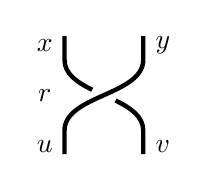
\begin{tikzpicture}
\pic[
  braid/.cd,
  number of strands=2,
  ultra thick,
  gap=0.1,
  name prefix=braid,
] {braid={a_{1}^{-1}}};
\node[] at (-.25,-.12) {$x$};
\node[] at (1.25,-.12) {$y$};
\node[] at (-.25,-1.4) {$u$};
\node[] at (1.25,-1.4) {$v$};
\node[] at (-.25,-.75) {$r$};
\end{tikzpicture}
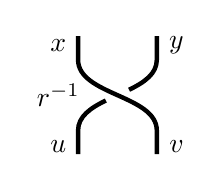
\begin{tikzpicture}
\pic[
  braid/.cd,
  number of strands=2,
  ultra thick,
  gap=0.1,
  name prefix=braid,
] {braid={a_{1}}};
\node[] at (-.25,-.12) {$x$};
\node[] at (1.25,-.12) {$y$};
\node[] at (-.25,-1.4) {$u$};
\node[] at (1.25,-1.4) {$v$};
\node[] at (-.25,-.75) {$r^{-1}$};
\end{tikzpicture}
\caption{Any row or column determines the whole square.}
\label{fig:braid}
\end{figure}

\begin{example}
If the map $(x,y)\mapsto(\sigma_x(y),\tau_y(x))$ satisfies the Yang--Baxter equation, then 
so does $(x,y)\mapsto (\tau_x(y),\sigma_y(x))$. 
\end{example}

\begin{example}
\label{exa:Lyubashenko}
Let $X$ be a non-empty set and $\sigma$ and $\tau$ be 
bijections on $X$ such that $\sigma\circ\tau=\tau\circ\sigma$. Then 
$(X,r)$, where $r(x,y)=(\sigma(y),\tau(x))$, is a non-degenerate solution. 
This is known as the \emph{permutation solution} associated
with permutations $\sigma$ and $\tau$. 
%The solution $(X,r)$ is involutive 
%if and only if $\tau^{-1}=\sigma$. 
\end{example}
%
%\begin{example}
%\label{exa:Wada}
%Let $G$ be a group. Then $(G,r)$, where $r(x,y)=(xy^{-1}x^{-1},xy^2)$, is a solution. 
%\end{example}

\begin{example}
\label{exa:Venkov}
Let $G$ be a group. Then $(G,r)$, where $r(x,y)=(xyx^{-1},x)$, is a solution. 
%It is involutive if and only if $G$ is abelian. 
\end{example}

The now prove the main theorem of the chapter. The result
shows an intriguing connection between group actions and non-degenerate solutions. It 
was proved by Lu, Yan and Zhu. 

\begin{theorem}
\label{thm:LYZ}
Let $G$ be a group and let $\xi\colon G\times G\to G$, $\xi(x,y)=x\rhd y$,
be a left action of $G$ on itself, and 
let $\eta\colon G\times G\to G$, $\eta(x,y)=x\lhd y$, 
be a right action of $G$ on itself. If the compatibility condition
\[
uv=(u\rhd v)(u\lhd v)
\]
holds for all $u,v\in G$, then the pair $(G,r)$, where 
\[
r\colon G\times G\to G\times G,\quad
r(u,v)=(u\rhd v,u\lhd v)
\]
is a solution. 
\end{theorem}

\begin{proof}
We write $r_1=r\times\id$ and $r_2=\id\times r$. Let
\[
r_1r_2r_1(u,v,w)=(u_1,v_1,w_1),\quad
r_2r_1r_2(u,v,w)=(u_2,v_2,w_2).
\]
The compatibility condition implies that $u_1v_1w_1=u_2v_2w_2$. 
So we need to prove that $u_1=u_2$ and $v_1=v_2$. From Lemma~\ref{lem:YB}
we note that
\begin{align*}
&u_1=(u\rhd v)\rhd ( (u\lhd v)\rhd w),
&&w_1=(u\lhd v)\lhd w,\\
&u_2=u\rhd (v\rhd w),
&&w_2=(u\lhd (v\rhd w))\lhd (v\lhd w).
\end{align*}
Using the compatibility condition and the fact that $\xi$ is a left action, 
\begin{align*}
    &u_1=((u\rhd v)(u\lhd v))\rhd w=(uv)\rhd w=u\rhd (v\rhd w)=u_2.
\end{align*}
Similarly, since $\eta$ is a right action, 
\[
w_2=u\lhd ((v\rhd w)(v\lhd w))=u\lhd (vw)=(u\lhd v)\lhd w=w_1.
\]

To prove that $r$ is invertible we proceed as follows. 
Write $r(u,v)=(x,y)$, thus $u\rhd v=x$, $u\lhd v=y$ and $uv=xy$. Since 
\begin{align*}
& (y\rhd v^{-1})u=(y\rhd v^{-1})(y\lhd v^{-1})=yv^{-1}=x^{-1}u,
\end{align*}
it follows that $y\rhd v^{-1}=x^{-1}$, i.e. $v^{-1}=y^{-1}\rhd x^{-1}$. Similarly, 
\[
v(u^{-1}\lhd x)=(u^{-1}\rhd x)(u^{-1}\lhd x)=u^{-1}x=vy^{-1}
\]
implies that $u^{-1}=y^{-1}\lhd x^{-1}$. Clearly 
$r^{-1}=\zeta (i\times i) r (i\times i) \zeta$,
is the inverse of $r$, where $\zeta(x,y)=(y,x)$ and $i(x)=x^{-1}$. 
\end{proof}

\begin{proposition}
Under the assumptions of Theorem~\ref{thm:LYZ}, 
if $r(x,y)=(u,v)$, then 
\[
r(x^{-1},y^{-1})=(u^{-1},v^{-1}),
\quad
r(x^{-1},u)=(y,v^{-1}),
\quad
r(v,y^{-1})=(u^{-1},x).
\]
\end{proposition}

\begin{proof}
In the proof of Theorem~\ref{thm:LYZ} we found that 
the inverse of the map $r$ is given by $r^{-1}=\zeta (i\times i) r (i\times i) \zeta$,
where $\zeta(x,y)=(y,x)$ and $i(x)=x^{-1}$. It follows that $r(x^{-1},y^{-1})=(u^{-1},v^{-1})$.  
To prove the equality $r(x^{-1},u)=(y,v^{-1})$ we proceed as follows. Since $r(x,y)=(u,v)$, it 
follows that $x\triangleright y=u$. Then $x^{-1}\triangleright u=y$ and
hence $r(x^{-1},u)=(y,z)$ for some $z\in G$. 
Since $xy=uv$ and $x^{-1}u=yz$, it follows that $yt=yv^{-1}$. Then 
$z=v^{-1}$. Similarly one proves $r(v,y^{-1})=(u^{-1},x).$
\end{proof}

\section*{Exercises}

\begin{prob}
\label{prob:Wada}
Let $G$ be a group. Prove that the following maps satisfy the set-theoretic YBE:
\begin{enumerate}[label=\alph*)]
\item $r(x,y)=(y,x^{-1})$.
\item $r(x,y)=(y^{-1},x^{-1})$.
\item $r(x,y)=(xyx,x^{-1})$.
\item $r(x,y)=(x^2y,y^{-1}x^{-1}y)$.	
\end{enumerate}	
\end{prob}

\begin{prob}
\label{prob:Wada_racks}
	Let $G$ be a group. Prove that the following maps satisfy the set-theoreic YBE:
	\begin{enumerate}[label=\alph*)]
	\item $r(x,y)=(x^myx^{-m},x)$.
	\item $r(x,y)=(xy^{-1}x,x)$.
\end{enumerate}	
\end{prob}

\begin{prob}
\label{prob:D_n}
Let $n\geq2$ and $X=\Z/(n)$ be the ring of integers modulo $n$. Prove that
the map $r(x,y)=(2x-y,x)$ satisfy the the set-theoretic YBE.  	
\end{prob}


\begin{prob}
Let $G$ be a group and $f\in\Aut(G)$. Prove that 
the map $r(x,y)=(f(y),f(y)^{-1}xy)$ satisfy the set-theoretic YBE.	
\end{prob}



%\begin{prob}
%Let $X$ be a \framebox{finite} non-empty set and $r\colon X\times X\to X\times X$, $(x,y)\mapsto (\sigma_x(y),\tau_y(x))$, be a map.
%Prove that $(X,r)$ is a solution if and only if 
%the maps $\sigma_x\colon X\to X$ are bijective for all $x\in X$,
%$r^2=\id_{X\times X}$ and 
%\[
%\sigma_x\circ\sigma_{\sigma^{-1}_x(y)}=\sigma_y\circ\sigma_{\sigma^{-1}_y(x)}
%\]
%for all $x,y\in X$. 
%\end{prob}
%
%
%\begin{prob}
%Prove that if $(X,r)$ be a solution...? \framebox{FIXME}
%\end{prob}
%
%\begin{prob}
%\label{prob:perm_group}
%Let $(X,r)$ be a solution. Prove that $\mathcal{G}(X,r)\simeq\langle (\sigma_x,\tau^{-1}_x):x\in X\rangle$. 
%\end{prob}


\section*{Notes}

\index{Gateva--Ivanova, T.}
\index{Van den Bergh, M.}
The first papers where set-theoretic solutions are studied are those of Etingof, Schedler and Soloviev~\cite{MR1722951} 
and Gateva--Ivanova and Van den Bergh~\cite{MR1637256}. 
Both papers deal with non-degenerate involutive solutions, i.e. solutions
$(X,r)$ where $r^2=\id$.  

%\index{Rump, W.}
\index{Drinfeld, V.}
\index{Wada, M.}
\index{Lyubashenko, V.}
In~\cite{MR1183474}, Drinfeld attributes Example~\ref{exa:Lyubashenko} to 
Lyubashenko. 

\index{Lu, J--H.}
\index{Yan, M.}
\index{Zhu, Y--C.}
\index{Etingof, P.}
\index{Schedler, T.}
\index{Soloviev, A.}
Theorem~\ref{thm:LYZ} goes back to Lu, Yan and Zhu, see~\cite{MR1769723}.
Similar results can be found in the work of Etingof, Schedler and Soloviev~\cite{MR1722951} 
for involutive solutions 
and in Soloviev's paper~\cite{MR1809284}.

Exercises~\ref{prob:Wada} and~\ref{prob:Wada_racks} 
appear in the work of Wada~\cite{MR1167178} on representations of braid groups. 
The solutions of Exercises~\ref{prob:Wada_racks} and~\ref{prob:D_n} 
are particular cases of a more general type of set-theoretic solutions that we will study in 
Chapter~\ref{racks}.  
%Proposition~\ref{pro:Rump} was proved by Rump~\cite{MR2278047}. 
%a similar example appears in the appendix of~\cite{MR1722951}. 
 


\chapter{Anillos radicales}

\index{Braza!asociativa}
Diremos que una braza es asociativa si la operación $(x,y)\mapsto
x*y=\lambda_x(y)-y$ es asociativa. Recordemos que en toda braza
vale la siguiente igualdad
\begin{align}
    \label{eq:(aob)*c}
    &(a+a*b+b)*c=(a\circ b)*c=a*(b*c)+b*c+a*c.
\end{align}

\begin{lemma}
	Si $A$ es una braza de tipo abeliano asociativa, entonces 
	\[
		(-a)*b=-(a*b)
	\]
	para todo $a,b\in A$. En particular, $(-a)\circ b=2b-(a\circ b)$ para todo $a,b\in A$. 
\end{lemma}

\begin{proof}
    Por la igualdad~\eqref{eq:(aob)*c} y la
    asociatividad, 
	\begin{align*}
	    (a*(-a))*b &= 
	    (a*(-a)+a+(-a))*b\\
	    &=a*( (-a)*b)+(-a)*b+a*b\\
	    &=(a*(-a))*b+(-a)*b+a*b,
    \end{align*}
    lo que implica que $(-a)*b=-(a*b)$. La segunda afirmación se obtiene
    entonces inmediatamente. 
\end{proof}

\begin{lemma}
Si $A$ es una braza de tipo abeliano, valen las siguientes
afirmaciones:
\begin{enumerate}
    \item $a*0=0*a=0$,
    \item $a*(-b)=-(a*b)$,
    \item $a*(b-c)=a*b-a*c$,
    \item $a*(b_1+\cdots+b_n)=a*b_1+\cdots+a*b_n$,
    %\sum_{i=1}^nb_i=\sum_{i=1}^na*b_i$,
\end{enumerate}
\end{lemma}

\begin{exercise}
Demuestre que en toda braza de tipo abeliano vale
que 
\[
    a*\left(\sum_{i=1}^nb_i-\sum_{j=1}^mc_j\right)=\sum_{i=1}^na*b_i-\sum_{j=1}^ma*c_j,
\]
y que esta fórmula puede rescribirse como
\begin{align}
\label{eq:Lau}
a\circ \left(\sum_{i=1}^n b_i-\sum_{j=1}^mc_j\right)
=\sum_{i=1}^n a\circ b_i-\sum_{j=1}^ma\circ c_j+(m-n+1)a.
\end{align}
\end{exercise}

% \begin{proof}
% Demostremos la última afirmación. Como $A$ es de tipo abeliano, 
% \begin{align*}
%     a*(b_1+\cdots+b_n-c_1-\cdots-c_m) &=
%     a*( (b_1+\cdots+b_n)-(c_1+\cdots+c_m))\\
%     &=a*(b_1+\cdots+b_n)-a*(c_1+\cdots+c_m)\\
%     &=\sum_{i=1}^na* b_i-\sum_{j=1}^ma*c_j.\qedhere
% \end{align*}
% \end{proof}

% Observemos que el lema anterior implica que vale la siguiente
% fórmula


\begin{theorem}
    \label{thm:Lau}
	Si $A$ es una braza de tipo abeliano asociativa, entonces $A$ es un anillo radical. 	
\end{theorem}

\begin{proof}
    Necesitamos demostrar que $A$ es una braza a derecha. 
	Como $A$ es asociativa, $(a*b)*c=a*(b*c)$ para todo $a,b,c\in A$. Rescribimos la asociatividad entre $a,b,c\in A$ como
	\[
	(a\circ b-a-b)\circ c-(a\circ b-a-b)-c
	=a\circ (b\circ c-b-c)-a-(b\circ c-b-c),
	\]
	que es equivalente a la igualdad 
	\[
	a'\circ ( (a\circ b-a-b)\circ c-a\circ b)
	=a'\circ ( a\circ (b\circ c-b-c)-a-a-b\circ c+2c).
	\]
	Si usamos la fórmula~\eqref{eq:Lau} en el miembro 
	de la derecha con $n=1$ y $m=2$ y en el miembro izquierdo
	con $n=m=3$, 
	\[
	a'\circ (a\circ b-a+(-b))=b+a'\circ(-b)
	\]
	La fórmula~\eqref{eq:Lau} ahora con $n=2$ y $m=1$ implica que
	la asociatividad de $A$ es equivalente a la identidad 
	\begin{equation}
	    \label{eq:asociatividad}
		(b+a'\circ (-b))\circ c+c=b\circ c+a'\circ(-b)\circ c.
	\end{equation}
	Sean $b,c\in A$. Si $d\in A$ existe $a\in a$ tal que $d=a'\circ (-b)$. La fórmula~\eqref{eq:asociatividad} 
	implica entonces que
	\[
	(b+d)\circ c+c=b\circ c+d\circ c,
	\]
	que es lo que queríamos demostrar.
\end{proof}

\section{Brazas biláteras}

Veamos qué podemos decir de las brazas biláteras cuyo grupo aditivo no necesariamente es abeliano.
Nos será de utilidad el siguiente lema.

\begin{lemma}
Si $A$ es una braza bilátera, entonces cada conjugación 
multiplicativa 
$\gamma_c\colon A\to A$, $a\mapsto c'\circ a\circ c$, es un automorfismo del grupo aditivo de $A$.
\end{lemma}

\begin{proof}
Simplemente hay que observar que
\[
\gamma_c(a+b)=c'\circ(a+b)\circ c=c'(a\circ c-c+a\circ c)=c'\circ a+c'\circ b=\gamma_c(a)+\gamma_c(b)
\]
y el lema queda demostrado. 
\end{proof}

El lema anterior implica que todo subgrupo característico del aditivo de una braza bilátera será
un ideal.

\begin{proposition}
Si $A$ es una braza bilátera finita con grupo aditivo resoluble, entonces
el grupo multiplicativo de $A$ es también resoluble.
\end{proposition}

\begin{proof}
Supongamos que la proposición es falsa y sea $A$ un contraejemplo minimal. Por el teorema de Etingof, Schedler
y Soloviev sabemos que $(A,+)$ no es un grupo abeliano. 
Sea entonces $I=[A,A]_+$. Como $I$ es característico en $(A,+)$, el lema anterior implica que $I$ es un ideal de $A$. Los brazas $I$ y $A/I$ son biláteras y 
tiene grupos aditivos resolubles. La minimalidad de $A$, entonces, implica que 
los grupos multiplicativos de $I$ y $A/I$ son también resolubles. Luego $(A,\circ)$ es resoluble, una contradicción.
\end{proof}

\begin{proposition}
Si $A$ es una braza biláera tal que $(A,+)$ es finitamente generado y residualmente finito, entonces
$(A,\circ)$ es también residualmente finito. 
\end{proposition}

\begin{proof}
Sin pérdidad de generalidad podemos suponer que $A$ es una braza infinita. 
Sea $a\in A$ un elemento no nulo. Como $(A,+)$ es residualmente finito, existe un subgrupo normal $N$ 
de $(A,+)$ de índice finito $n$ tal que $x\not\in N$. Como $(A,+)$ es finitamente generado, existen
solamente finitos subgrupos de $(A,+)$ de índice $n$. La intersección 
$I=\cap_{\varphi\in\Aut(A,+)}\varphi(N)$ 
es un subgrupo característico de $(A,+)$ no trivial (de lo contrario $A$ sería finita), de índice finito y tal que  $x\not\in I$. Como $I$ es característico, es un ideal de $A$ y luego, en particular, $I$ es un subgrupo 
normal del multiplicativo de $A$, de índice finito y tal que $x\not\in I$.
\end{proof}

\section*{Notas}

El teorema~\ref{thm:Lau} fue demostrado por Ivan Lau en \verb+arXiv:1811.04894+ e independientemente por Michael Kinyon. Responde a una pregunta
hecha por Ferran Cedó, Tatiana Gateva--Ivanova y Agata Smoktunowicz en 
\cite[Question 2.1(2)]{MR3818285}.

\chapter{Racks}

\begin{definition}
\label{defn:rack}
\index{Rack}
A \emph{rack} is a pair $(X,\triangleright)$, 
where $X$ is a non-empty set and 
$X\times X\to X$, $(x,y)\mapsto x\triangleright y$, is a binary operation on $X$ such that
the maps $\rho_y\colon X\to X$, $x\mapsto x\triangleleft y$, are bijective for all $y\in X$, and 
\begin{equation}
\label{eq:rack}
(x\triangleleft y)\triangleleft z=(x\triangleleft z)\triangleleft (y\triangleleft z)
\end{equation}
for all $x,y,z\in X$.
\end{definition}

Racks are used in low-dimensional topology~\cite{MR3379534}, singularities~\cite{MR975077} 
and in the classification of finite-dimensional pointed Hopf algebras~\cite{MR1994219}.

\begin{example}
\index{Rack!trivial}
    Let $X$ be a set. Then $x\triangleleft y=x$ turns $X$ into a rack. 
    This is the \emph{trivial rack} on $X$. 
\end{example}

\begin{example}
    \index{Rack!dihedral}
    Let $X=\Z/n$. Then $x\triangleleft y=2y-x$ turns $X$ into a rack. This is 
    the \emph{dihedral rack} of size $n$. 
\end{example}

\begin{example}
    \index{Rack!Alexander}
    Let $A$ be an abelian group and $f\in\Aut(A)$. Then 
    \[
    x\triangleleft y=(\id-f)(y)+f(x)
    \]
    turns $A$ into a rack. These racks 
    are known as the \emph{Alexander racks}.
\end{example}

\begin{definition}
    \index{Rack!homomorphism}
    \index{Rack!isomorphism}
    \index{Homomorphism!of racks}
    Let $X$ and $Z$ be racks. 
    A \emph{rack homomorphism} between the racks $X$ and $Z$ is a map $f\colon X\to Z$ such that 
    $f(x\triangleleft y)=f(x)\triangleleft f(y)$ for all $x,y\in X$. 
    An \emph{isomorphism} of racks is a bijective rack homomorphism. 
\end{definition}

For $n\in\N$, let $r(n)$ be the number of isomorphism classes of racks of size
$n$. Some values of $r(n)$ appear in Table~\ref{tab:racks}, see for example~\cite{MR3957904}.  

\begin{table}[H]
\centering
\caption{Enumeration of non-isomorphic racks.}
\begin{tabular}{|c|cccccccccccc|}
\hline
$n$ & 2 & 3 & 4 & 5 & 6 & 7 & 8 & 9 & 10 & 11 & 12 & 13\tabularnewline
\hline
$r(n)$ & 2 & 6 & 19 &74&353 & 2080 & 16023 & 159526 & 2093244 & 36265070 & 836395102 & 25794670618\tabularnewline
\hline
\end{tabular}
\label{tab:racks}
\end{table}

\begin{proposition}
\label{pro:Venkov}
Let $X$ be a non-empty set and $X\times X\to X$, $(x,y)\mapsto x\triangleleft y$ be a binary operation on $X$. Then
$r(x,y)=(y,x\triangleleft y)$ is a solution if and only if $(X,\triangleleft)$ is a rack. 
\end{proposition}

\begin{proof}
The map $r$ satisfies $(r\times\id)(\id\times r)(r\times\id)=(\id\times r)(r\times\id)(\id\times r)$ if and only
if~\eqref{eq:rack} holds for all $x,y,z\in X$. The solution $(X,r)$ is non-degenerate if 
the maps $X\to X$, $x\mapsto x\triangleleft y$, are bijective. 
\end{proof}

The connection between racks and solutions goes deeper than 
the phenomenon appearing in Proposition~\ref{pro:Venkov}. 


\begin{proposition}
    \label{pro:derived}
    Let $(X,r)$ be a solution. Then 
    \begin{equation}
    \label{eq:derived}
    x\triangleleft y=\sigma_y\tau_{\sigma_x^{-1}(y)}(x)=\sigma_y\widehat{\sigma}^{-1}_y(x)
    \end{equation}
    turns $X$ into a rack and each $\sigma_x$ is a rack homomorphism. 
    Moreover, $(X,r)$ is involutive if and only if the rack $(X,\triangleleft)$ is trivial. 
\end{proposition}

\begin{proof}
    Since $r(x,\sigma_x^{-1}(y))=(y,\tau_{\sigma_x^{-1}(y)}(x))$, 
    it follows that 
    $\widehat{\sigma}_y^{-1}(x)=\tau_{\sigma_x^{-1}(y)}(x)$ 
    for all $x,y\in X$. Hence the second equality of~\eqref{eq:derived} holds. 
    
    To prove that each $\tau_z$ is a rack homomorphism it is enough to show that
    \[
    \sigma_x(y)\triangleleft \sigma_x\sigma_y(z)=\sigma_x(y\triangleleft\sigma_y(z))
    \]
    for all $x,y\in X$. Write $r(x,y)=(u,v)$. On the one hand, by 
    Lemma~\ref{lem:YB}, 
    \begin{align*}
        \sigma_x(y)\triangleleft \sigma_x\sigma_y(z)
        &=u\triangleleft \sigma_u\sigma_v(z)
        =\sigma_{\sigma_u\sigma_v(z)}\tau_{\sigma_{\tau_y(x)}(z)}\sigma_x(y)
        =\sigma_{\sigma_x\sigma_y(z)}\sigma_{\tau_{\sigma_y(z)}(x)}\tau_z(y).
    \end{align*}
    On the other hand, 
    \begin{align*}
        \sigma_x(y\triangleleft\sigma_y(z)) 
        &=\sigma_x\sigma_{\sigma_y(z)\tau_z(y)}
        =\sigma_{\sigma_x\sigma_y(z)}\sigma_{\tau_{\sigma_y(z)}(x)}\tau_z(y).
    \end{align*}
    
    By Proposition~\ref{pro:Venkov}, in order to prove that $(X,\triangleright)$ is a rack it is enough to show that
    $r(x,y)=(y,x\triangleleft y)$ satisfies the YBE. For that purpose, we demonstrate that 
    the map $J\colon X^3\to X^3$, $J(x,y,z)=(x,\sigma_x(y),\sigma_x\sigma_y(z))$ 
    is invertible and 
    satisfies 
    \[
    (\id\times s)\circ J=J\circ(\id\times r),
    \quad
    (s\times\id)\circ J=J\circ(r\times\id).
    \]
    The map $(x,y,z)\mapsto (x,\sigma_x^{-1}(y),\sigma_{\sigma_x^{-1}(y)}^{-1}\sigma_x^{-1}(z))$ is the inverse of $J$. 

    Since $\sigma_x$ is a rack homomorphism, 
    \begin{align*}
    \sigma_x(y)\triangleleft \sigma_x\sigma_y(z)
    &=\sigma_x(y\triangleleft \sigma_y(z))
    =\sigma_x\sigma_{\sigma_y(z)}\tau_{\sigma_y^{-1}\sigma_y(z)}(y)
    =\sigma_x\sigma_{\sigma_y(z)}\tau_z(y)
    \end{align*}
    Then it follows that 
    \begin{align*}
        (\id\times s)J(x,y,z)
        &=(\id\times s)(x,\sigma_x(y),\sigma_x\sigma_y(z))\\
        &=(x,\sigma_x\sigma_y(z),\sigma_x(y)\triangleleft \sigma_x\sigma_y(z))\\
        &=(x,\sigma_x\sigma_y(z),\sigma_x\sigma_{\sigma_y(z)}\tau_z(y))\\
        &=J(x,\sigma_y(z),\tau_z(y))\\
        &=J(\id\times r)(x,y,z).
    \end{align*}
    Similarly one proves that $(s\times\id)\circ J=J\circ (r\times\id)$.  
    This implies that $(X,s)$ is a solution and 
    hence $(X,\triangleleft)$ is a rack by Proposition~\ref{pro:Venkov}. 

    If $(X,r)$ is involutive, 
    then $x\triangleleft\sigma_x(y)=\sigma_{\sigma_x(y)}\tau_y(x)=x$ by~\eqref{eq:involutive}. 
    Conversely, if $x\triangleleft y=x$ for all $x,y\in X$,
    then $r$ is involutive, as 
    \[
    r^2(x,\sigma_x^{-1}(y))=r(y,\sigma_y^{-1}(x))=(x,\sigma_x^{-1}(y)).\qedhere
    \]
\end{proof}

%\begin{definition}
\index{Solution!derived rack}
The rack constructed in Proposition~\ref{pro:derived} is 
known as the \emph{derived solution} of $(X,r)$. 
%\end{definition}
There is a dual version of the derived rack:

\begin{proposition}
    \label{pro:derived_dual}
    Let $(X,r)$ be a solution. Then 
    \[
    x\blacktriangleleft y=\tau_y\sigma_{\tau_x^{-1}(y)}(x)=\tau_y\widehat{\tau}^{-1}_y(x)
    \]
    turns $X$ into a rack and each $\tau_x$ is a rack homomorphism. 
\end{proposition}

\begin{proof}
    Since $(X,r)$ is a solution, then so is $(X,r_0)$, where 
    $r_0(x,y)=(\tau_x(y),\sigma_y(x))$. Then the claim follows 
    from Proposition~\ref{pro:derived_dual} applied to 
    the solution $(X,r_0)$.
\end{proof}

In general, the racks constructed in Propositions~\ref{pro:derived} 
and~\ref{pro:derived_dual} are different:

\begin{example}
Let $X=\{1,\dots,5\}$ and $(X,r)$ be the solution given by
\begin{align*}
&\sigma_1=\id, && \sigma_2=\id, && \sigma_3=\id, && \sigma_4=(13)(45), &&\sigma_5=(12)(45),\\
&\tau_1=\id, && \tau_2=\id, && \tau_3=\id, && \tau_4=(23)(45), &&\tau_5=(23)(45).
\end{align*}
On the one hand the derived rack of $(X,r)$ is given by the permutations 
\begin{align*}
&\sigma_1\widehat{\sigma}_1^{-1}=\sigma_2\widehat{\sigma}_2^{-1}=\sigma_3\widehat{\sigma}_3^{-1}=\id,
&&\sigma_4\widehat{\sigma}_4^{-1}=(132),
&&\sigma_5\widehat{\sigma}_5^{-1}=(123).
\end{align*}
On the other hand, the dual derived rack by 
\begin{align*}
&\tau_1\widehat{\tau}_1^{-1}=\tau_2\widehat{\tau}_2^{-1}=\tau_3\widehat{\tau}_3^{-1}=\id,
&&\tau_4\widehat{\tau}_4^{-1}=(123),
&&\tau_5\widehat{\tau}_5^{-1}=(132).
\end{align*}
% [ [ (), (), (), (1,3)(4,5), (1,2)(4,5) ], [ (), (), (), (2,3)(4,5), (2,3)(4,5) ] ]
%[ [ (), (), (), (2,3)(4,5), (2,3)(4,5) ], [ (), (), (), (1,3)(4,5), (1,2)(4,5) ] ]
% [ (), (), (), (1,3,2), (1,2,3) ]
% [ (), (), (), (1,2,3), (1,3,2) ]
\end{example}

We now prove that the racks 
of Propositions~\ref{pro:derived} 
and~\ref{pro:derived_dual} are isomorphic. 
We shall need a lemma. 



\begin{lemma}
\label{lem:T_invertible}
Let $(X,r)$ be a solution. 
The map $T\colon X\to X$, $x\mapsto\sigma_x^{-1}(x)$, is invertible with
inverse $U\colon X\to X$, $x\mapsto\tau^{-1}_x(x\blacktriangleleft x)$. 
\end{lemma}

\begin{proof}
Let $x\in X$ and $y=U(x)=\tau^{-1}_x(x\blacktriangleleft x)$. 
Then $\tau_x(y)=x\blacktriangleleft x=\tau_x\widehat{\tau}^{-1}_x(x)$ and hence
$y=\widehat{\tau}^{-1}_x(x)$. Then $\widehat{\tau}_x(y)=x$ and 
\[
r^{-1}(y,x)=(\widehat{\sigma}_y(x),x)=(z,x),
\]
where $z\in X$ is such that $\sigma_z(x)=y$. By Lemma~\ref{lem:YB}, $\sigma_y=\sigma_z$. Then 
it follows that $x=\sigma^{-1}_y(y)=T(y)$. Therefore $y=U(x)=U(T(y))$.

To prove that $T(U(x))=x$, first note that 
\[
r(\tau^{-1}_x(x),x)=(\sigma_{\tau^{-1}_x(x)}(x),x)
\]
and Lemma~\ref{lem:YB} imply that $\sigma_{\tau^{-1}_x(x)}=\sigma_{\sigma_{\tau^{-1}_x(x)}(x)}$. Now
\begin{align*}
T(U(x))&=T(\tau^{-1}_x(x\blacktriangleleft x))=T(\sigma_{\tau^{-1}_x(x)}(x))\\
&=\sigma^{-1}_{\sigma_{\tau^{-1}_x(x)}(x)}\sigma_{\tau^{-1}_x(x)}(x)
=\sigma^{-1}_{\tau^{-1}_x(x)}\sigma_{\tau^{-1}_x(x)}(x)=x.\qedhere
\end{align*}
\end{proof}

There is version of Proposition~\ref{pro:T} for arbitrary solutions. 
A similar result appears in Exercise~\ref{prob:variationT}.



\begin{proposition}
    Let $(X,r)$ be a solution. Then $T\colon X\to X$, $x\mapsto\tau_x^{-1}(x)$, is a bijective
    map such that 
    \[
      T\circ\tau_y=\widehat{\sigma}^{-1}_y\circ T,
      \quad
      T\circ \widehat{\tau_y}=\sigma^{-1}_{y}\circ T
    \]
    and $T(x\blacktriangleleft y)=T(x)\triangleleft T(y)$ for all $x,y\in X$. 
\end{proposition}

\begin{proof}
    Lemma~\ref{lem:T_invertible} proves that $T$ is bijective. 
    We now compute 
    \begin{align*}
        T\tau_y(x) &= 
        \sigma^{-1}_{\tau_y(x)}\tau_y(x)
        =\sigma^{-1}_{\tau_y(x)}\sigma^{-1}_{\sigma_x(y)}\sigma_{\sigma_x(y)}\tau_y(x)\\
        &=\sigma^{-1}_y\sigma^{-1}_x\sigma_{\sigma_x(y)}\tau_y(x)
        =\sigma^{-1}_y\sigma_x^{-1}(x\triangleleft\sigma_x(y))
        =\sigma^{-1}_y(T(y)\triangleleft y)
        =\widehat{\sigma}^{-1}_yT(x).
    \end{align*}

    Since $\widehat{\tau}_y(x)=\sigma^{-1}_{\widehat{\sigma}_x(y)}(x)$, Lemma~\ref{lem:YB} implies that 
    \begin{align*}
        T\widehat{\tau_y}(x) 
        &=\sigma^{-1}_{\widehat{\tau}_y(x)}\widehat{\tau}_y(x)
        =\sigma^{-1}_{\widehat{\tau}_y(x)}\sigma^{-1}_{\widehat{\sigma}_x(y)}
        =\sigma^{-1}_{y}\sigma^{-1}_{x}(x)
        =\sigma^{-1}_{y}T(x).
    \end{align*}
    These formulas imply that
    \begin{equation}
        \label{eq:T_rack}
        T\circ\tau_y\circ\widehat{\tau}_y^{-1}
        =\widehat{\sigma}^{-1}_y\circ T\circ \widehat{\tau}^{-1}_y
        =\widehat{\sigma}^{-1}_y\circ \sigma_y\circ T.
    \end{equation}

    We evaluate Equality~\eqref{eq:T_rack} on $X$. On the one hand, 
    $T(x\blacktriangleleft y)=T\sigma_x\widehat{\sigma_x}^{-1}(y)$.
    On the other hand,
    \begin{align*}
        \widehat{\sigma}_y^{-1}\sigma_yT(x)
        &=\sigma_y^{-1}\sigma_y\widehat{\sigma}_y^{-1}\sigma_yT(x)
        =\sigma_y^{-1}(\sigma_yT(x)\triangleleft y)=T(x)\triangleleft T(y).\qedhere
    \end{align*}
\end{proof}


%If $(X,r)$ is a solution, the map $r\colon X\times X\to X\times X$ is invertible. Write 
% \[
% r^{-1}(x,y)=(\widehat{\sigma}_x(y),\widehat{\tau}_y(x)).
% \]
% Since $(X,r^{-1})$ is a solution, Lemma~\ref{lem:YB} implies that 
% the following formulas hold:
% \[
% \widehat{\tau}_y\widehat{\tau_x}=\widehat{\tau}_{\tau_y(x)}\widehat{\tau}_{\sigma_x(y)},
% \quad
% \widehat{\sigma}_x\widehat{\sigma_y}=\widehat{\sigma}_{\sigma_x(y)}\widehat{\sigma}_{\tau_y(x)}.
% \]
% Since $r(\tau^{-1}_y(x),y)=(\sigma_{\tau^{-1}_y(x)}(y),x)$, 
% it follows that 
% \[
% \widehat{\tau}_x\sigma_{\tau^{-1}_y(x)}(y)=y.
% \]
% for all $x,y\in X$. Moreover, 
% \[
% x\triangleright y=\tau_x\sigma_{\tau^{-1}_y(x)}(y)=\tau_x\widehat{\tau}^{-1}_x(y)
% \]
% for all $x,y\in X$. 

%We first need a lemma. 

% \begin{proposition}
%     Let $(X,r)$ be a solution and let $(X,\triangleright)$ be its derived rack. 
%     Then 
%     \[
%     T\circ \sigma_x=\tau_x^{-1}\circ\rho_x\circ T
%     \]
%     for all $x\in X$, where $T\colon X\to X$, $T(y)=\tau_y^{-1}(y)$, and 
%     $\rho_x\colon X\to X$, $\rho_x(y)=x\triangleright y$.
% \end{proposition}

% \begin{proof}
% By using Lemma~\ref{lem:YB} we compute 
% \begin{align*}
%     T\sigma_x(y) &= \tau^{-1}_{\sigma_x(y)}\sigma_x(y)
%     =\tau^{-1}_{\sigma_x(y)}(\tau^{-1}_{\tau_y(x)}(\tau_y(x)\triangleright y))\\
%     &=\tau^{-1}_{\sigma_x(y)}\tau^{-1}_{\tau_y(x)}(\tau_y(x)\triangleright y))\\
%     &=\tau^{-1}_{x}\tau^{-1}_{y}(\tau_y(x)\triangleright y))\\
%     &=\tau^{-1}_{x}(x\triangleright T(y)).\qedhere 
% \end{align*}
% \end{proof}

% \begin{proposition}
% \label{pro:T_general}
% Let $(X,r)$ be a solution. 
% The map $T\colon X\to X$, $x\mapsto\sigma_{\tau_x^{-1}(x)}(x)$, is invertible with
% inverse $U\colon X\to X$, $x\mapsto\sigma^{-1}_x(x)$. 
% \end{proposition}

% \begin{proof}
% Let $(X,\triangleright)$ be the derived rack of $(X,r)$. Then 
% $T(x)=\tau_x^{-1}(x\triangleright x)$. Since 
% $r(\tau_z^{-1}(z),z)=(\sigma_{\tau^{-1}_z(z)}(z),z)$, 
% \begin{equation}
%     \label{eq:Ttrick}
%     \sigma_{\tau^{-1}_z(z)}\circ\sigma_z=\sigma_{\sigma_{\tau^{-1}_z(z)}(z)}\circ\sigma_z
% \end{equation}
% holds for all $z\in X$ by 
% Lemma~\ref{lem:YB}. On the one hand, 
% \begin{align*}
%     U(T(x)) 
%     &= U(\sigma_{\tau^{-1}_x(x)}(x))
%     =\sigma^{-1}_{\sigma_{\tau^{-1}_x(x)}(x)}\sigma_{\tau^{-1}_x(x)}(x)=x
% \end{align*}
% because $\sigma_{\tau^{-1}_x(x)}=\sigma_{\sigma_{\tau^{-1}_x(x)}(x)}$ by~\eqref{eq:Ttrick}. 

% Now let $x,y\in X$ be such that $U(x)=y$. Since $r^{-1}(\sigma_x(y),\tau_y(x))=(x,y)$, 
% it follows that $\widehat{\tau}_{\tau_y(x)}\sigma_x(y)=y$ and that 
% $\widehat{\tau}_{\tau_y(x)}=\widehat{\tau_y}$. Then
% \[
% \widehat{\tau}_y(x)=\widehat{\tau}_{\tau_y(x)}(x)=\widehat{\tau}_{\tau_y(x)}\sigma_x(y)=y
% \]
% and hence $\widehat{\tau}^{-1}_y(y)=x$. Now $y\triangleright y=\tau_y\widehat{\tau}^{-1}_y(y)=\tau_y(x)$ and therefore
% \[
% T(y)=\tau_y^{-1}(y\triangleright y)=x.\qedhere
% \]
% \end{proof}

As it happens in the involutive case, there is a nice combinatorial structure that describes  
a solution. 

\begin{definition}
\index{Skew cycle set}
\index{Skew cycle set!non-degenerate}
\label{defn:skewCS}
A \emph{skew cycle set} is a triple $(X,\triangleleft,\cdot)$, where $X$ is a non-empty set, 
$(X,\triangleleft)$ is a rack and
$X\times X\to X$, $(x,y)\mapsto x\cdot y$, is a binary operation on $X$ such that the maps 
$X\to X$, $y\mapsto x\cdot y$, are bijective rack homomorphisms, and 
\begin{equation}
\label{eq:skew_CS}
(x\cdot y)\cdot (x\cdot z)=(y\cdot (x\triangleleft y))\cdot (y\cdot z)
\end{equation}
for all $x,y,z\in X$. A skew cycle set $(X,\triangleleft,\cdot)$ is said to be 
non-degenerate if the map $X\times X$, $x\mapsto x\cdot x$, is bijective.
\end{definition}

\framebox{FIXME}

\begin{definition}
\index{Homomorphism!of skew cycle sets}
Let $X$ and $Z$ be skew cycle sets. 
A \emph{homomorphism} between the cycle sets $X$ and $Z$ is a 
map $f\colon X\to Z$ such that $f(x\cdot y)=f(x)\cdot f(y)$ for all $x,y\in X$. An \emph{isomorphism} of cycle sets
is a bijective homomorphism of cycle sets. 
\end{definition}

Cycle sets and cycle set homomorphisms form a category. 
It is possible to prove that the category of 
solutions is equivalent to the category of cycle sets, 
see Exercise~\ref{prob:cycle_sets}. 


Theorem~\ref{thm:CS} can be generalized to arbitrary solutions.

\begin{theorem}
\label{thm:skewCS}
There exists a bijective correspondence between solutions 
and non-degenerate skew cycle sets. 
\end{theorem}

\begin{proof}
Let $(X,r)$ be a solution and $(X,\triangleleft)$ its derived rack. We will prove that 
the operation $x\cdot y=\sigma_x^{-1}(y)$ turns $(X,\triangleleft)$ into a skew cycle set.
By Proposition~\ref{pro:derived}, 
the 
maps $X\to X$, $y\mapsto x\cdot y$, are bijective rack homomorphisms. 

On the one hand, since $r(x,\sigma_x^{-1}(y))=(y,\tau_{\sigma_x^{-1}(y)}(x))$, 
\begin{align*}
(x\cdot y)\cdot (x\cdot z)
&=\sigma_x^{-1}(y)\cdot\sigma_x^{-1}(z)
=\sigma_{\sigma_x^{-1}(y)}^{-1}\sigma_x^{-1}(z)\\
&=\left(\sigma_x\circ\sigma_{\sigma_x^{-1}(y)}\right)^{-1}(z)
=\left(\sigma_y\circ\sigma_{\tau_{\sigma_x^{-1}(y)}(x)}\right)^{-1}(z).
\end{align*}
On the other hand, 
\begin{align*}
(y\cdot (x\triangleleft y))\cdot (y\cdot z)
&=\sigma_y^{-1}(\sigma_y\tau_{\sigma_x^{-1}(y)}(x))\cdot\sigma_y^{-1}(z)\\
&=\sigma^{-1}_{\tau_{\sigma_x^{-1}(y)}(x)}\sigma_y^{-1}(z)
=\left(\sigma_y\circ\sigma_{\tau_{\sigma^{-1}_x(y)}(x)}\right)^{-1}(z).
\end{align*}

Now we prove the converse statement. 
For $x,y\in X$ let 
\[
\sigma_x(y)=x*y,
\quad
\tau_y(x)=\sigma_{\sigma_x(y)}^{-1}(x\triangleleft\sigma_x(y)), 
\]
where $x*y=z$ if and only if $x\cdot z=y$. 
Since $X$ is a skew cycle set, each $\sigma_x$ is bijective. Let us prove that the $\tau_x$ are bijective. 
Equality~\eqref{eq:skew_CS} with $y=\sigma_x(z)$ implies that
\[
\sigma_z^{-1}\sigma_x^{-1}=\sigma^{-1}_{\sigma_x^{-1}(y)}\sigma_x^{-1}
=\sigma^{-1}_{\sigma_y^{-1}(x\triangleleft y)}\sigma_y^{-1}
=\sigma^{-1}_{\sigma^{-1}_{\sigma_x(z)}(x\triangleleft\sigma_x(z))}\sigma^{-1}_{\sigma_x(z)}
=\sigma^{-1}_{\tau_z(x)}\sigma^{-1}_{\sigma_x(z)}
\]
for all $x,z\in X$. 
Since each $\sigma_x$ is a rack homomorphism, 
\[
\tau_y(x)=\sigma^{-1}_{\sigma_x(y)}(x\triangleleft\sigma_x(y))
=\sigma^{-1}_{\sigma_x(y)}\sigma_x(\sigma^{-1}_x(x)\triangleleft y)
=\sigma_{\tau_y(x)}\sigma_y^{-1}(\sigma_x^{-1}(x)\triangleleft y).
\]
Therefore $T\circ\tau_y=\sigma_y^{-1}\circ\rho_y\circ T$, where $T\colon X\to X$, $T(x)=x\cdot x$ 
and $\rho_y\colon X\to X$, $\rho_y(x)=x\triangleleft y$ are bijective maps. In particular, 
$\tau_y$ is bijective for all $y\in X$. 

Now we prove that...
\framebox{solution?}

\framebox{invertible?}
\end{proof}

Theorem~\ref{thm:skewCS} can be used to construct small solutions, see Table~\ref{tab:non_involutive}.

\begin{table}[H]
\centering
\caption{Enumeration of non-involutive solutions.}
\begin{tabular}{|c|ccccccc|}
\hline
$n$ & 2 & 3 & 4 & 5 & 6 & 7 & 8\tabularnewline
\hline
$s(n)$ & 2 & 21 & 253 & 3519 & 100071 & 4602720 & 422449480\tabularnewline
\hline
\end{tabular}
\label{tab:non_involutive}
\end{table}

\section*{Exercises}

% \begin{prob}
%     \label{prob:Venkov}
%     Let $X$ be a set and $X\times X\to X$, $(x,y)\to x\triangleright y$. Prove that 
%     the pair $(X,s)$, where
%     $s(x,y)=(x\triangleright y,x)$, is a solution if and only if $(X,\triangleright)$ is a rack. 
%     Prove that
% \end{prob}
\begin{prob}
    \label{prob:xx}
    Prove that $x\triangleright x=x\blacktriangleright x$ for all $x\in X$. 
\end{prob}

\begin{prob}
    \label{prob:tau_hat}
    Prove that $\widehat{\tau}_x(y\triangleright z)=\widehat{\tau}_x(y)\triangleright \widehat{\tau}_x(z)$ for all $x,y,z\in X$. 
\end{prob}

\begin{prob}
    \label{prob:variationT}
    Let $(X,r)$ be a solution and let $(X,\triangleright)$ be its derived rack. 
    Prove that 
    \[
    T\sigma_x(y)=\tau_x^{-1}(x\triangleright T(y))
    \]
    for all $x\in X$, where $T\colon X\to X$, $T(y)=\tau_y^{-1}(y)$. 
\end{prob}

\begin{prob}
\label{prob:guitar}
Let $(X,r)$ be a solution and $(X,\triangleright)$ its derived rack. Let $T_2(x,y)=(\tau_y(x),y)$ and
$T_{n+1}=Q_n\circ (T_n\times\id)$ for $n\geq2$, where 
\[
Q_n(x_1,\dots,x_{n+1})=(\tau_{x_{n+1}}(x_1),\dots,\tau_{x_{n+1}}(x_n),x_{n+1}).
\]
Prove that $T_n\circ r_{i,i+1}=s_{i,i+1}\circ T_n$ for all $n\geq2$ and $i\in\{1,\dots,n-1\}$. 
\end{prob}

\section*{Open problems}

\begin{problem}
\label{problem:racks14}
Enumerate isomorphism classes of racks of size 14. 
\end{problem}

\begin{problem}
Enumerate non-involutive solutions of size $\geq9$. 
\end{problem}


\section*{Notes}

% Definition~\ref{defn:rack} is that of a \emph{left rack}. 
% A \emph{right rack} is defined as a pair $(X,\triangleleft)$, where $X$ is a non-empty set, 
% $X\times X\to X$, $(x,y)\mapsto x\triangleleft y$, is 
% a binary operation on $X$ such that the maps $x\mapsto x\triangleleft y$, are bijective and 
% \[
% (x\triangleleft y)\triangleleft z=(x\triangleleft z)\triangleleft (y\triangleleft z)
% \]
% for all $x,y,z\in X$. 
% As we did in Proposition~\ref{pro:derived}, one proves that $x\triangleleft y=...$ turns $X$ into a 
% right rack. This leads to the right derived solution of $(X,r)$. 
%According to Drinfeld, Exercise~\label{prob:Venkov} 
A particular family of racks turns out to be useful in combinatorial know theory. A quandle
is a rack $(X,\triangleleft)$ such that $x\triangleleft x=x$ for all $x\in X$. 

In~\cite{MR1183474}, Drinfeld attributes Proposition~\ref{pro:Venkov} to Venkov. 

There are several papers on the enumeration of isomorphic classes of finite racks~\cite{MR3665565,MR3118951,MR3904151}. 
Estimations on the number of finite
racks of size $n$ appear in~\cite{MR3118951}. 

The numbers of Table~\ref{tab:non_involutive} were computed using 
Theorem~\ref{thm:skewCS} essentially with the same technique used to construct involutive solutions~\cite{AMV}. 
The construction of non-involutive solutions of size 9 seems to be feasible with these methods. 
However, it should be noted that a huge number of solutions is expected. 

Exercises~\ref{prob:xx} and~\ref{prob:tau_hat} appear in~\cite{MR3974961}. 

The map $J$ of Exercise~\ref{prob:guitar} is known as the \emph{guitar map}. 
It was first considered by Etingof, Schedler and
Soloviev in~\cite{MR1722951} for involutive solutions. The construction was extended to non-involutive solutions
by Soloviev in~\cite{MR1809284} and Lu, Yan and Zhu in~\cite{MR1769723}. In~\cite{MR3374524} Dehornoy
used the inverse of the guitar map to develop his right-cyclic calculus and to
obtain short proofs for results on the structure group of involutive solutions. 
In~\cite{MR1994219} Andruskiewitsch and Graña use the guitar map to study certain isomorphisms of Nichols algebras. 
A particular case of the guitar map also appears in the work of Przytycki~\cite{MR2906433}. 

The derived rack of a solution was first defined in the work of Soloviev~\cite{MR1809284}. Most of the properties
of the derived racks mentioned in this chapter were proved in~\cite{MR3974961}.

Problem~\ref{problem:racks14} appears in~\cite{MR3957904}. 


\chapter{Skew braces}
\label{braces}

% Braces were introduced by Rump in~\cite{MR2278047} to study set-theoretical involutive
% solutions of the Yang--Baxter equation. The following definition of~\cite{MR3647970} 
% generalizes braces to the non-involutive setting.
\section*{Skew braces and the Yang--Baxter equation}

By convention, an additive group $A$ will be a (not necessarily abelian) group 
with a binary operation $(a,b)\mapsto a+b$. The 
identity of $A$ will be denoted by $0$ and the inverse of an element $a$ will be denoted by $-a$. 

\begin{definition}
    \label{def:brace}
	\index{Skew brace}
	\index{Skew brace!multiplicative group}
	\index{Skew brace!additive group}
	A \emph{skew left brace} is a triple $(A,+,\circ)$, where $(A,+)$ and $(A,\circ)$ 
	are (not necessarily abelian) 
	groups and 
	\begin{equation}
	    \label{eq:compatibility}
	    a\circ(b+c)=(a\circ b)-a+(a\circ c)
	\end{equation}
	holds for all $a,b,c\in A$. The groups 
	$(A,+)$ and $(A,\circ)$ are respectively 
	the \emph{additive} and \emph{multiplicative} group
	of the skew left brace $A$.
\end{definition}

We write $a'$ to denote the inverse of $a$ with respect to the circle operation $\circ$. 

Skew right braces are defined similarly, one needs 
to replace~\eqref{eq:compatibility} by 
\[
(a+b)\circ c=a\circ c-c+b\circ c.
\]
There is a bijective correspondence between skew left braces and skew right braces, 
see Exercise~\ref{prob:left_right}. For that reason, 
a skew brace will always mean a skew left brace. 

\begin{definition}
    Let $\mathcal{X}$ be a family of groups. A skew brace $A$ is said to be
    of $\mathcal{X}$-type if its additive group belongs to $\mathcal{X}$.
\end{definition}

One particularly interesting family of skew braces is the family of \emph{skew braces of abelian type}, 
that is skew braces with abelian additive group. 
Skew braces of abelian type were introduced by Rump in~\cite{MR2278047} to study involutive solutions to the Yang--Baxter equation. 
In the literature, skew braces of abelian type are called \emph{left braces}. 

\begin{example}
	\label{exa:trivial}
	\index{Skew brace!trivial}
	Let $A$ be an additive group. Then $A$ is a skew brace with
	$a\circ b=a+b$ for all $a,b\in A$. 
	A skew brace $(A,+,\circ)$ such that $a\circ b=a+b$ for all $a,b\in A$ is
    said to be \emph{trivial}. 
	Similarly, the
   operation $a\circ b=b+a$ turns $A$ into a skew brace. 
\end{example}

\begin{example}
	\label{exa:times}
	\index{Direct product!of skew braces}
	Let $A$ and $B$ be skew braces. Then $A\times B$ with 
	\[
		(a,b)+(a_1,b_1)=(a+a_1,b+b_1),\quad
		(a,b)\circ (a_1,b_1)=(a\circ a_1,b\circ b_1),
	\]
	is a skew brace. This is the {\em direct product} of the skew braces $A$ and $B$. 
\end{example}

\begin{example}
	\label{exa:sd}
	Let $A$ and $M$ be additive groups and let $\alpha\colon A\to\Aut(M)$ be a
	group homomorphism. Then $M\times A$ with 
	\[
	(x,a)+(y,b)=(x+y,a+b),
	\quad
	(x,a)\circ (y,b)=(x+\alpha_a(y),a+b)
	\]
	is a skew brace. Similarly, $M\times A$ with
	\[
	(x,a)+(y,b)=(x+\alpha_a(y),a+b),\quad
	(x,a)\circ (y,b)=(x+y,b+a)
	\]
	is a skew brace. 
\end{example}

\begin{example}
  \label{exa:s3c6}
  Let $A=\Sym_3$ be the symmetric group in three letters. Write $A$ as an additive group. 
  Let $\lambda\colon A\to\Sym_A$ 
  be the map given by
  \begin{align*}
    &\lambda_{\id}=\lambda_{(123)}=\lambda_{(132)}=\id,\\
    &\lambda_{(12)}=\lambda_{(23)}=\lambda_{(13)}=\text{conjugation by $(23)$}.
  \end{align*}
  It is easy to check that $\lambda_{a+\lambda_a(b)}=\lambda_a\lambda_b$
  for all $a,b\in A$. Hence $A$ with the circle operation defined by $a\circ b=a+\lambda_a(b)$, for all $a,b\in A$, is a skew brace by Exercise~\ref{prob:equivalences}. 
  Since the transposition $(12)$ has order
  six in the multiplicative group of $A$, it follows that the additive group of $A$ is isomorphic to $\Sym_3$ and
  the multiplicative group of $A$ is isomorphic to the cyclic group of order six. 
\end{example}

The following example is motivated by the paper~\cite{MR1178147}.

\begin{example}
    \label{exa:WX}
    Let $A$ be an additive group
	and $B$ and $C$ be subgroups of $A$ such that $B\cap C=\{ 0\}$ and $A=B+C$. In this case, one says that $A$ admits an {\em exact factorization} through the subgroups $B$ and $C$.  Thus each $a\in A$ can be written in a unique
	way as $a=b+c$, for some $b\in B$ and $c\in C$.  The map
	\[
		B\times C\to A,\quad
		(b,c)\mapsto b-c,
	\]
	is bijective. Using this map we transport the group structure of the direct
	product $B\times C$ into the set $A$. That is, for $a=b+c\in A$, where $b\in B$ and $c\in C$, and
	$a_1\in A$, let 
	\begin{align*}
		a\circ a_1&=b+a_1+c.
	\end{align*}
	Then $(A,\circ)$ is a group isomorphic to $B\times C$. Moreover, if $x,y\in A$, 
	then 
	\begin{align*}
	a\circ x-a+a\circ y=b+x+c-(b+c)+b+y+c=b+x+y+c=a\circ (x+y),
	\end{align*}
	and therefore $(A,+,\circ)$ is a skew brace. 
\end{example}

% \begin{proof} The map $\eta\colon B\times C\to A$, $\eta(b,c)=bc^{-1}$, is
%   bijective.  Since $\eta$ is bijective and $a\circ
%   a'=\eta(\eta^{-1}(a)\eta^{-1}(a'))$, it follows that $(A,\circ)$ is a group
%   isomorphic to the direct product $B\times C$. To prove that $A$ is a skew
%   brace it remains to show~\eqref{eq:compatibility}. Let $a=bc\in BC$ and
%   $a',a''\in A$. Then \begin{align*} (a\circ a')a^{-1}(a\circ a'')
%     &=(ba'c)a^{-1}(ba''c)\\ &=ba'c(c^{-1}b^{-1})ba''c\\ &=ba'a''c\\ &=a\circ
%     (a'a'').  \end{align*} This completes the proof.  \end{proof}

We now give concrete some examples of the previous construction. 

\begin{example}
  \label{exa:QR}
  Let $n$ be a positive integer.  Let $A\in M_n(\C)$. If 
  \[A=\left(\begin{array}{cccc}
  a_{1,1}&a_{1,2}&\ldots &a_{1,n}\\
  a_{2,1}&a_{2,2}&\ddots&\vdots\\
  \vdots&\ddots&\ddots&a_{n-1,n}\\
  a_{n,1}&\ldots&a_{n,n-1}&a_{n,n}\end{array}\right),\]
  we define
  \[A^*=\bar{A}^t= =\left(\begin{array}{cccc}
  \bar a_{1,1}&\bar a_{2,1}&\ldots &\bar a_{n,1}\\
  \bar a_{1,2}&\bar a_{2,2}&\ddots&\vdots\\
  \vdots&\ddots&\ddots&\bar a_{n,n-1}\\
  \bar a_{1,n}&\ldots&\bar a_{n-1,n}&\bar a_{n,n}\end{array}\right),\]
  where $\overline{a+bi}=a-bi$, for all $a,b\in\R$.
  The group $\GL_n(\C)$ admits an
  exact factorization through the subgroups $U(n)$ and $T(n)$, where $U(n)=\{ A\in\GL_n(\C)\mid AA^*=I\}$
  is the unitary group and $T(n)$ is the group of upper triangular matrices
  with positive diagonal entries.  Therefore there exists a skew brace with additive group 
  isomorphic to $\GL_n(\C)$ and multiplicative group isomorphic to $U(n)\times T(n)$.  
\end{example}

The following examples appeared in the theory of 
Hopf--Galois \textcolor{blue}{structures}, see~\cite[Corollary 1.1]{MR3425626}.

\begin{example} 
	\label{exa:a5a4c5}
	The alternating simple group $\Alt_5$ admits an exact factorization
  through the subgroups 
  $A=\langle (123),(12)(34)\rangle\cong\Alt_4$ and 
  $B=\langle(12345)\rangle\cong C_5$.  
  There exists a skew brace with additive group isomorphic to $\Alt_5$ and multiplicative
  group isomorphic to $\Alt_4\times C_5$. 
\end{example}

\begin{example} 
	\label{exa:PSL27S4C7}
  The simple group $\PSL_2(7)=\SL_2(7)/Z(\SL_2(7))$ admits an exact factorization through the subgroups \[A=\left\langle\left(\begin{array}{cc}
  0&1\\
  -1&-1\end{array}\right)Z(\SL_2(\C)),\left(\begin{array}{cc}
  1&-2\\
  1&-1\end{array}\right)Z(\SL_2(\C))\right\rangle\cong\Sym_4\] and \[B=\left\langle\left(\begin{array}{cc}
  1&1\\
  0&1\end{array}\right)Z(\SL_2(\C))\right\rangle\cong C_7.\] 
  Hence there exists a skew brace with additive
  group isomorphic to $\PSL_2(7)$ and multiplicative group isomorphic to 
  $\Sym_4\times C_7$.  
\end{example}

\begin{lemma}
    \label{lem:basic}
	Let $A$ be a skew brace. Then the following properties hold:
    \begin{enumerate}
        \item $0=1$.  
        \item $a\circ(-b+c)=a-(a\circ b)+(a\circ c)$, for all $a,b,c\in A$.
        \item $a\circ(b-c)=(a\circ b)-(a\circ c)+a$, for all $a,b,c\in A$.
    \end{enumerate}
\end{lemma}

\begin{proof}
		The first claim follows from the compatibility condition~\eqref{eq:compatibility} with
		$c=1$.  To prove the second claim let $d=b+c$.
		Then~\eqref{eq:compatibility} becomes 
		\[
		a\circ d =a\circ b-a+a\circ (-b+d)
		\]
		and the claim follows. The third claim is
		proved similarly.
\end{proof}

\begin{proposition}
\label{pro:lambda}
    Let $A$ be a skew brace. For each $a\in A$, the map
    \[
        \lambda_a\colon A\to A,\quad
        b\mapsto -a+(a\circ b),
    \]
    is an automorphism of the additive group $(A,+)$. Moreover, the map 
    $\lambda\colon (A,\circ)\to\Aut(A,+)$, $a\mapsto\lambda_a$, is a group homomorphism. 
\end{proposition}

\begin{proof}
The inverse of $\lambda_a$ is given by $\lambda^{-1}_a\colon A\to A$, $b\mapsto a'\circ (a+b)$. To prove
that $\lambda_a\in\Aut(A,+)$ we note that
\[
\lambda_a(b+c)=-a+a\circ(b+c)=-a+a\circ b-a+a\circ c=\lambda_a(b)+\lambda_a(c).
\]
Note that $\lambda_a(b)=-a+a\circ b=a\circ (a'+b)$, for all $a,b\in A$. Hence 
%To prove that $\lambda$ is a group homomorphism, we 
%use Lemma~\ref{lem:basic} to obtain
\begin{align*}
\lambda_a(\lambda_b(c))&=a\circ (a'+b\circ (b'+c))=-a+a\circ b\circ (b'+c)\\
&=-a+a-a\circ b+a\circ b\circ c=-a\circ b+a\circ b\circ c=\lambda_{a\circ b}(c).\qedhere    
\end{align*}
\end{proof}

If $A$ is a skew brace, then 
the map $\lambda$ in the previous proposition yields a left action from $(A,\circ)$ on $(A,+)$ by automorphisms. 
There is also a right action of $(A,\circ)$ on the set $A$.

\begin{proposition}
\label{pro:mu}
    Let $A$ be a skew brace. For each $a\in A$, the map
    \[
        \mu_a\colon A\to A,\quad
        b\mapsto \lambda_b(a)'\circ b\circ a,
    \]
    is bijective. Moreover, the map 
    $\mu\colon (A,\circ)\to\Sym_A$, $a\mapsto\mu_a$, satisfies $\mu_b\circ\mu_a=\mu_{a\circ b}$, for all $a,b\in A$. 
\end{proposition}

\begin{proof}
    Note that
    \[\mu_a(b)=\lambda_b(a)'\circ b\circ a=(b\circ (b'+a))'\circ b\circ a=(b'+a)'\circ a,\]
    for all $a,b\in A$. Hence $\mu_a$ is bijective and
    \[\mu_a^{-1}(b)=((b\circ a')'-a)'=(a\circ b'-a)'=(b'+a')'\circ a',\]
    for all $a,b\in A$. Now we have
    \begin{align*}
        \mu_b(\mu_a(c))&=\mu_b((c'+a)'\circ a)=(a'\circ (c'+a)+b)'\circ b\\
        &=(a'\circ c'-a'+b)'\circ b=(a'\circ (c'+a\circ b))'\circ b\\
        &=(c'+a\circ b)'\circ a\circ b=\mu_{a\circ b}(c),
    \end{align*}
    for all $a,b,c\in A$. Therefore the result follows.
%    Let $a,b,c\in A$. To prove that $\mu$ is a group anti-homorphism, we compute
%    \begin{align*}
%    &\mu_{b\circ a}(c)=\lambda_c(b\circ a)'\circ c\circ b\circ a
%    \shortintertext{and}
%    &\mu_a\mu_b(c)=\mu_a(\lambda_c(b)'\circ c\circ b)
%    =\lambda_{\lambda_c(b)'\circ c\circ b}(a)'\circ \lambda_c(b)'\circ c\circ b\circ a.
%    \end{align*}
%    Using the formulas~\eqref{eq:formulas} and Proposition \ref{pro:lambda}, 
%    \begin{align*}
%    \lambda_c(b\circ a)'&=\lambda_c(b+\lambda_b(a))'=(\lambda_c(b)+\lambda_{c\circ b}(a))'\\
%    &=(\lambda_c(b)\circ %\lambda^{-1}_{\lambda_c(b)}\lambda_{c\circ b}(a))'
%    =\lambda_{\lambda_c(b)'\circ c\circ b}(a)'\circ \lambda_c(b)',
%    \end{align*}
%    which proves that $\mu$ is an anti-homomorphism. 
%    
%    To compute the inverse of $\mu_b$ we proceed as follows. Since $a'\circ (-a)=2a$ by Lemma~\ref{lem:basic}, 
%    \begin{align*}
%    (\lambda_a(b)'\circ a\circ b)'&=b'\circ (a'\circ \lambda_a(b))\\
%    &=b'\circ (a'\circ (-a+a\circ b))
%    =b'\circ (a'+b)=b'\circ a'-b.
%    \end{align*}
%    From this one immediately obtains that $\mu_b^{-1}(a)=(b\circ a'-b)'$. 
\end{proof}


Let $A$ be a skew brace. 
\index{Commutator identities!for braces}
Proposition \ref{pro:lambda} implies that 
\begin{align}
\label{eq:formulas}
&a\circ b = a+\lambda_a(b),
&&a+b=a\circ \lambda^{-1}_a(b),
&&\lambda_a(a')=-a
\end{align}
hold for $a,b\in A$. Moreover, if 
\[
    a*b=\lambda_a(b)-b=-a+a\circ b-b,
\]
then the following identities are easily verified:
\begin{align}
&a*(b+c)=a*b+b+a*c-b,\\
&(a\circ b)*c=(a*(b*c))+b*c+a*c.
\end{align}
These last two identities are similar to the usual
\emph{commutator identities}.

 \begin{definition}
 	\index{Homomorphism!of skew braces}
 	A map $f\colon A\to B$ between two skew braces $A$ and $B$ is a {\em homomorphism of skew braces} if $f(x\circ y)=f(x)\circ f(y)$ and $f(x+y)=f(x)+f(y)$, for all $x,y\in A$.  The \emph{kernel} of $f$ is
     \[
         \ker f=\{a\in A:f(a)=0\}.
     \]
 \end{definition}

A bijective homomorphism of skew braces is an isomorphism. An automorphism of a skew brace $A$ is an isomorphism from the skew brace $A$ to it self. Two skew braces $A$ and $B$ are isomorphisc if there exist an isomorphism $f\colon A\rightarrow B$. We write $A\cong B$ to denote that the skew braces $A$ and $B$ are isomorphic.

\begin{proposition}
\label{prop:semidirect} 
\index{Skew brace!semidirect product} Let $A,B$ be skew braces. Let $\alpha\colon (B,\circ)\rightarrow \Aut(A,+,\circ)$ be a homomorphism of groups. Define two operations on $A\times B$ by
\[ (a_1,b_1)+(a_2,b_2)=(a_1+a_2,b_1+b_2)\text{ and }(a_1,b_1)\circ (a_2,b_2)=(a_1\circ\alpha_{b_1}(a_2),b_1\circ b_2),\]
where $\alpha_{b_1}=\alpha(b_1)$, for all $a_1,a_2\in A$ and $b_1,b_2\in B$. Then $(A\times B,+,\circ)$ is a skew brace. This skew brace is the {\em semidirect product} of the skew brace $A$ by $B$ via $\alpha$, and it is denoted by $A\rtimes_{\alpha}B$.
\end{proposition}

\begin{proof}
    Note that $(A\times B,+)$ is the direct product of the groups $(A,+)$ and $(B,+)$, and $(A\times B,\circ)$ is the semidirect product of the group $(A,\circ)$ by $(B,\circ)$ via $\alpha$. Hence it is enough to check the compatibility condition.
    Let $a_1,a_2,a_3\in A$ and $b_1,b_2,b_3\in B$. We have
    \begin{align*}
        (a_1,b_1)\circ &((a_2,b_2),(a_3,b_3))\\
        =&(a_1,b_1)\circ (a_2+a_3,b_2+b_3)\\
        =&(a_1\circ \alpha_{b_1}(a_2+a_3),b_1\circ (b_2+b_3))\\
        =&(a_1\circ (\alpha_{b_1}(a_2)+\alpha_{b_1}(a_3)),b_1\circ b_2-b_1+b_1\circ b_3)\\
        =&(a_1\circ \alpha_{b_1}(a_2)-a_1+a_1\circ\alpha_{b_1}(a_3)),b_1\circ b_2-b_1+b_1\circ b_3)\\
        =&(a_1\circ \alpha_{b_1}(a_2),b_1\circ b_2)-(a_1,b_1)+(a_1\circ\alpha_{b_1}(a_3)),b_1\circ b_3)\\
        =&(a_1,b_1)\circ (a_2,b_2)-(a_1,b_1)+(a_1,b_1)\circ (a_2,b_3).
    \end{align*}
Therefore the result follows.
\end{proof}
%Braces and brace homomorphisms form a category.  

%\begin{example}
%        \label{exa:trivial}
%        Let $(A,\cdot)$ be a group. Then $A$ is a skew left brace with
%        $a\circ b=ab$ for all $a,b\in A$.  Similarly, $a\star b=ba$ defines a
%        skew left brace structure over $A$. These braces are isomorphic
%        if and only if $(A,\cdot)$ is abelian.
%\end{example}
%
%\begin{example}
%	\label{exa:sd}
%    Let $A$ and $B$ be groups and let $\alpha\colon A\to\Aut(B)$ be a
%    group homomorphism. Assume that $A$ is abelian. Then $A\times B$ has a
%    skew left brace structure given by
%    \begin{align*}
%        &(a,b)(a',b')=(aa',b\alpha_a(b')),\\
%        &(a,b)\circ(a',b')=(aa',bb'),
%    \end{align*}
%    where $a,a'\in A$ and $b,b'\in B$. 
%\end{example}
%
%\begin{example}
%    \label{exa:WX}
%    This example is motivated by the paper of Weinstein and
%	Xu on the Yang--Baxter equation, see~\cite{MR1178147}. Let $A$ be a group
%	and $A_+,A_-$ be subgroups of $A$ such that $A$ admits a \emph{unique
%	factorization} as $A=A_+A_-$. Thus each $a\in A$ can be written in a unique
%	way as $a=a_+a_-$ for some $a_+\in A_+$ and $a_-\in A_-$.  The map
%	\[
%		A_+\times A_-\to A,\quad
%		(a_+,a_-{)}\mapsto a_+(a_{-})^{-1},
%	\]
%	is bijective. Using this map we transport the group structure of the direct
%	product $A_+\times A_-$ into the set $A$. For $a=a_+a_-\in A$ and
%	$b=b_+b_-\in A$ let 
%	\begin{align*}
%		a\circ b&=a_+ba_-.
%	\end{align*}
%	Then $(A,\circ)$ is a group. Furthermore, $A$ is a
%	skew left brace.
%\end{example}



% \begin{exa}
%   \label{exa:trivial}
%   Let $A$ be a group. Then $a\circ b=ab$ gives a skew brace. Similarly, the
%   operation $a\circ b=ba$ turns $A$ into a skew brace. 
% \end{exa}



% Lemma~\ref{lem:lambda} justifies the following definition:

% \begin{defn}
% 	\label{def:structure}
% 	Let $A$ be a skew brace. The \emph{crossed group} of $A$ is defined as
% 	the group $\Gamma(A)=(A,\cdot)\rtimes(A,\circ)$ with multiplication 
%     \[
%     (a,x)(b,y)=(a\lambda_x(b),x\circ y).
%     \]
% \end{defn}

% The following two propositions were proved by Bachiller in the case of braces of abelian type, 
% see \cite[Lemma 2.4]{Bachiller3} and~\cite[Proposition 2.3]{MR3465351}.

% \begin{proposition}
% 	\label{lem:mu}
% 	Let $A$ be a skew brace and let 
% 	\[
% 	\mu\colon\Mul{A}\to\Sym_A,\quad
% 	\mu_b(a)=\overline{\lambda_a(b)}\circ a\circ b. 
% 	\]
% 	Then 
% 	$\mu_1=\id$ and $\mu_{a\circ b}=\mu_b\mu_a$ for all $a,b\in A$.
% \end{proposition}

% \begin{proof}
    
% \end{proof}

% \begin{proposition}
% \label{lem:Bachiller}
% Let $A$ be a group and $\lambda\colon A\to\Aut(A)$ be a map such that
% \begin{equation}
% \label{eq:lambda}
% \lambda_{a\lambda_a(b)}=\lambda_a\lambda_b,\quad a,b\in A.
% \end{equation}
% Then $A$ with $a\circ b=a\lambda_a(b)$ is a skew brace. 
% \end{proposition}

% %\begin{lem}
% %	The following statement hold:
% %	\begin{enumerate}
% %		\item Let $A$ be a skew brace. The map 
% %			\[
% %			\lambda\colon\Mul{A}\to\Aut\Add{A},\quad
% %			\lambda_a(b)=a^{-1}(a\circ b),
% %			\]
% %			is a group homomorphism.
% %		\item Let $A$ be a group and $\lambda\colon A\to\Aut(A)$ be a map such that
% %			\begin{equation}
% %				\label{eq:lambda}
% %				\lambda_{a\lambda_a(b)}=\lambda_a\lambda_b,\quad a,b\in A.
% %			\end{equation}
% %			Then $A$ with $a\circ b=a\lambda_a(b)$ is a skew brace. 
% %	\end{enumerate}
% %\end{lem}

% \begin{proof}
% 	The first claim is~\cite[Corollary 1.10]{MR3647970}. For the second claim see~\cite[Lemma 1.1.17]{BachillerTESIS}.
% \end{proof}

% The following lemma provides another useful tool for constructing skew braces.

% \begin{proposition}
% 	\label{lem:dual}
% 	Let $\Mul{A}$ be a group and $\lambda\colon A\to\Sym_A$ be a group
% 	homomorphism.  Assume that 
% 	$\lambda_a(1)=1$ for all $a\in A$ and that
% 	\begin{equation}
% 		\label{eq:dual}
% 		\lambda_a(b\circ\lambda^{-1}_b(c))=\lambda_a(b)\circ\lambda^{-1}_{\lambda_a(b)}\lambda_a(c)
% 	\end{equation}
% 	for all $a,b,c\in A$. Then $A$  with 
% 	$ab=a\circ\lambda^{-1}_a(b)$ is a skew brace. 
% \end{proposition}

% \begin{proof}
% 	Note that Equation~\eqref{eq:dual} is equivalent to
% 	\begin{equation}
% 		\label{eq:better}
% 		\lambda_a^{-1}(bc)=\lambda_a^{-1}(b)\lambda_a^{-1}(c).
% 	\end{equation}
% 	We prove that the operation is associative:
% 	\begin{align*}
% 		a(bc) &= a\circ\lambda^{-1}_a(bc)
% 		=a\circ(\lambda^{-1}_a(b)\lambda^{-1}_a(c))\\
% 		&=a\circ\lambda^{-1}_a(b)\circ \lambda^{-1}_{a\circ \lambda^{-1}_a(b)}(c)
% 		=(ab)\circ\lambda^{-1}_{ab}(c)=(ab)c.
% 	\end{align*}

% 	The neutral element $1$ of $A$ is a right identity: $a1=a\circ\lambda^{-1}_a(1)=a\circ 1=a$. 
% 	The element $a^{-1}=\lambda_a(\overline{a})$ is a right inverse of $A$ since 
% 	\[
% 	aa^{-1}=a\circ\lambda^{-1}_a(a^{-1})=a\circ\lambda^{-1}_a\lambda_a(\overline{a})=a\circ\overline{a}=1.
% 	\]
% 	Therefore $\Add{A}$ is a group by~\cite[\S1.1.2]{MR1357169}. 

% 	The brace compatibility condition follows from Equation~\eqref{eq:better}:
% 	\begin{align*}
% 		&(a\circ b)a^{-1}(a\circ c)=(a\circ b)\lambda_a(c)=a\lambda_a(b)\lambda_a(c)=a\lambda_a(bc)=a\circ (bc).
% 	\end{align*}
% 	The lemma is proved. 
% \end{proof}

%\begin{exa}
%	Let $A_1,\dots,A_n$ be groups. Assume that 
%	for each $i\in\{2,\dots,n-1\}$ there is a group homomorphism 
%	$\rho_{i}\colon A_{i-1}\ltimes_{\rho_{i-1}} A_i\to\Aut(A_{i+1})$. 
%	Then the set $A_1\times\cdots\times A_n$ with
%	additive structure given by
%	\[
%	(a_1,\dots,a_n)\cdot(a_1',\dots,a_n')=(a_1a_1',\dots,a_n a_n')
%	\]
%	and multiplicative structure given by 
%	\begin{multline*}
%		(a_1,\dots,a_n)\circ (a_1',\dots,a_n')\\
%		=(a_1a_1',a_2\rho_1(a_1)(a_2'),a_3\rho_2(a_1,a_2)(a_3'),\dots,a_n\rho_{n-1}(a_1,\dots,a_{n-1})(a_n'))    
%	\end{multline*}
%	is a skew brace. This brace will be denoted by
%	\[
%	A_1\ltimes_{\rho_1} A_2\ltimes_{\rho_2}A_3\ltimes_{\rho_3}\cdots\ltimes_{\rho_{n-1}}A_n.
%	\]
%\end{exa}

\begin{lemma}\label{lem:homlambda}
    Let $A$ and $B$ be skew braces. A map $f\colon A\to B$ is a homomorphism of skew braces if and only if $f(a\circ b)=f(a)\circ f(b)$ and $f(\lambda_a(b))=\lambda_{f(a)}(f(b))$, for all $a,b\in A$.
\end{lemma}

\begin{proof}
    Let $a,b\in A$. Suppose that $f$ is a homomorphism of skew braces. Then
    \[ f(\lambda_a(b))=f(-a+a\circ b)=-f(a)+f(a)\circ f(b)=\lambda_{f(a)}(f(b)).\]
    Conversely, suppose that $f(x\circ y)=f(x)\circ f(y)$ and $f(\lambda_x(y))=\lambda_{f(x)}(f(y))$, for all $x,y\in A$. We have that 
    \[f(a+b)=f(a\circ\lambda_{a'}(b))=f(a)\circ f(\lambda_{a'}(b))=f(a)\circ \lambda_{f(a)'}(f(b))=f(a)+f(b).\]
    Therefore the result follows. 
\end{proof}



\begin{definition}
    \index{Skew brace!two sided}
	A skew brace $A$ is said to be a \emph{skew two-sided brace} if 
	\begin{equation}
	\label{eq:right_compatibility}
	(a+b)\circ c=a\circ c-c+b\circ c
	\end{equation}
	holds for all $a,b,c\in A$. 
\end{definition}

If $A$ is a skew two-sided brace, then 
\begin{align}
\label{eq:2sided}
&a\circ(-b)=a-a\circ b+a,
&&(-a)\circ b=b-a\circ b+b    
\end{align}
hold for all $a,b\in A$. The first equality holds for every skew brace and follows from Lemma~\ref{lem:basic}. 
The second equality follows from~\eqref{eq:right_compatibility}. 

\begin{example}
  Any skew brace with abelian multiplicative group is 
  two-sided.
\end{example}

\begin{example}
  Let $n\in\N$ be such that $n=p_1^{a_1}\cdots p_k^{a_k}$, where the $p_j$ are
  distinct primes, all $a_j\in\{1,2\}$ and $p_i^m\not\equiv 1\bmod{p_j}$ for
  all $i,j,m$ with $1\leq m\leq a_i$. Then every brace of size $n$ is a skew
  two-sided brace of abelian type, since every group of order $n$ is abelian, see for
  example~\cite{MR1786236}.  
\end{example}

\index{Jacobson!radical ring}
\index{Radical ring}
Skew two-sided braces of abelian type form an interesting family of rings without unit. 
% Those rings, known as radical rings, 
% were introduced by Jacobson in~\cite{MR12271}. In any ring $R$ the \emph{circle operation} 
% \[
% x\circ y=x+xy+y
% \]
% is always associative 
% and such that $x\circ 0=0\circ x=x$ for all $x\in R$. A non-unital ring (or \emph{rng}, for short) 
% $R$ is said to be a \emph{radical ring} if $(R,\circ)$ is a group. 
% In this case, following Jacobson's notation, the inverse of an element $x$ with respect to the circle operation is denoted by $x'$. 
% There are other characterizations of radical rings, see for example~\cite{MR3308118}.

% \begin{example}
%     The ring 
%     $R=\begin{pmatrix}
%     0 & \R & \R\\
%     0 & 0 & \R\\
%     0 & 0 & 0
%     \end{pmatrix}$ 
%     is  radical ring. 
% \end{example}

% \begin{example}
%     The ring $R=\left\{\frac{2x}{2y+1}:x,y\in\Z\right\}$ is a radical ring. In fact, 
%     \[
%     \left(\frac{2x}{2y+1}\right)'=\frac{2(-x)}{2(x+y)+1}.
%     \]
% \end{example}

Skew braces are a far reaching generalizations of radical rings. The following result was proved by Rump in~\cite{MR2278047}.

\begin{theorem}
\label{thm:radical}
    A skew brace of abelian type is two-sided if and only if it is a radical ring. 
\end{theorem}

\begin{proof}
    Assume first that $A$ is a skew two-sided brace of abelian type. Then $(A,+)$ is an abelian group. 
    Let us prove that the operation
    \[
    a*b=-a+a\circ b-b
    \]
    turns $A$ into a radical ring. Left distributivity follows from the compatibility condition:
    \begin{align*}
    a*(b+c)&=-a+a\circ (b+c)-(b+c)
    =-a+a\circ b-a+a\circ c-c-b=a*b+a*c.
    \end{align*}
    Similarly, since $A$ is two-sided, one proves $(a+b)*c=a*c+b*c$. It remains to show that the operation $*$
    is associative. On the one hand, using the first equality of~\eqref{eq:2sided} 
    and the compatibility condition, we write
    \begin{align*}
    a*(b*c)&=a*(-b+b\circ c-c)\\
    &=-a+a\circ(-b+b\circ c-c)-(-b+b\circ c-c)\\
    &=-a+a\circ (-b)-a+a\circ(b\circ c)-a+a\circ (-c)+c-b\circ c+b\\
    &=a\circ (b\circ c)-a\circ b-a\circ c-b\circ c+a+b+c,
    \end{align*}
    since the group $(A,+)$ is abelian. On the other hand, the second equality of~\eqref{eq:2sided} and
    Equality~\eqref{eq:right_compatibility} imply that
    \begin{align*}
    (a*b)*c &= (-a+a\circ b-b)*c=-(-a+a\circ b-b)+(-a+a\circ b-b)\circ c-c\\
    &=b-a\circ b+a+(-a)\circ c-c+(a\circ b)\circ c-c+(-b)\circ c-c\\
    &=(a\circ b)\circ c-a\circ b-a\circ c-b\circ c+a+b+c.
    \end{align*}
    It then follows that the operation $*$ is associative. 
    
    Conversely, if $A$ is a radical ring, say with ring multiplication $(a,b)\mapsto ab$, 
    then $a\circ b=a+ab+b$ turns $A$ into a skew two-sided brace 
    of abelian type. In fact, since $A$ is a radical ring, then 
    $(A,+)$ is an abelian group and $(A,\circ)$ is a group. Moreover, 
    \begin{align*}
        a\circ (b+c)=a+a(b+c)+(b+c)=a+ab+ac+b+c=a\circ b-a+a\circ c.
    \end{align*}
    Similarly ones proves $(a+b)\circ c=a\circ c-c+b\circ c$.
\end{proof}

\index{Brace!associative}
A skew brace is said to be \emph{associative} if the operation $(x,y)\mapsto
x*y=\lambda_x(y)-y$ is associative. In \cite[Question 2.1(2)]{MR3818285}, 
Cedó, Gateva--Ivanova and Smoktunowicz asked whether associative skew braces of abelian type are always radical rings. 
To answer this question, we need some lemmas. 

\begin{lemma}\label{lem:CGIS}
    If $A$ is an associative skew brace of abelian type, then $(-a)*b=-(a*b)$ 
	holds for all $a,b\in A$. In particular, $(-a)\circ b=2b-(a\circ b)$ for all $a,b\in A$. 
\end{lemma}

\begin{proof}
    The associativity implies that 
 	\begin{align*}
 	    (a*(-a))*b &= 
 	    (a*(-a)+a+(-a))*b=(a\circ (-a))*b\\
 	    &=a*( (-a)*b)+(-a)*b+a*b\\
 	    &=(a*(-a))*b+(-a)*b+a*b
     \end{align*}
     and therefore $(-a)*b=-(a*b)$. From this the result follows. 
\end{proof}

If $A$ is a skew brace of abelian type, then one proves by induction that 
\begin{align}
\label{eq:Lau}
    a\circ \left(\sum_{i=1}^n b_i-\sum_{j=1}^mc_j\right)
    =\sum_{i=1}^n a\circ b_i-\sum_{j=1}^ma\circ c_j+(m-n+1)a
\end{align}
holds for all $a,b,c\in A$, see Exercise~\ref{prob:Lau}. 

% \begin{lemma}
% If $A$ is a brace of abelian type, then 
% % \[
% %     a*\left(\sum_{i=1}^nb_i-\sum_{j=1}^mc_j\right)=\sum_{i=1}^na*b_i-\sum_{j=1}^ma*c_j,
% % \]
% \begin{align}
% \label{eq:Lau}
% a\circ \left(\sum_{i=1}^n b_i-\sum_{j=1}^mc_j\right)
% =\sum_{i=1}^n a\circ b_i-\sum_{j=1}^ma\circ c_j+(m-n+1)a.
% \end{align}
% \end{lemma}

% \begin{proof}

% \end{proof}

%The following result 
%answers \cite[Question 2.1(2)]{MR3818285}. 

\begin{theorem}
    \label{thm:Lau}
	If $A$ is an associative skew brace of abelian type, then $A$ is a radical ring. 
\end{theorem}

\begin{proof}
    We need to prove that the right compatibility condition holds. 
    Since $A$ is associative, $(a*b)*c=a*(b*c)$ for all $a,b,c\in A$. Write the associativity condition between $a,b,c\in A$ as
 	\[
 	(a\circ b-a-b)\circ c-(a\circ b-a-b)-c
 	=a\circ (b\circ c-b-c)-a-(b\circ c-b-c),
 	\]
 	which is equivalent to 
 	\[
 	a'\circ ( (a\circ b-a-b)\circ c-a\circ b)
 	=a'\circ ( a\circ (b\circ c-b-c)-a-a-b\circ c+2c).
 	\]
 	By Lemma \ref{lem:CGIS}, this is equivalent to
 	\[ a'\circ ( (a\circ b-a-b)\circ c-a\circ b)
 	=a'\circ ( a\circ (b\circ c-b-c)-a-a+(-b)\circ c).
 	\]
    By using the formula~\eqref{eq:Lau}, this is equivalent to  
 	\[
 	(b+a'\circ(-b))\circ c-b+a'=b\circ c-b-c+a'\circ (-b)\circ c+a'
 	\]
 	Hence the associativity of $(A,*)$ is equivalent to 
 	\begin{equation}
 	    \label{eq:asociatividad}
 		(b+a'\circ (-b))\circ c+c=b\circ c+a'\circ(-b)\circ c.
 	\end{equation}
 	Let $b,c\in A$. If $d\in A$, then there exists $a\in A$ such that $d=a'\circ (-b)$. Equality~\eqref{eq:asociatividad} 
    implies that 
 	\[
 	(b+d)\circ c+c=b\circ c+d\circ c.\qedhere
 	\]
\end{proof}


Now we show an associative skew brace that is not two-sided: 

\begin{example}
{\bf Ferran: si el ejemplo es demasiado técnico, entonces quizás es mejor escribir ``There are associative skew braces that are not two-sided, see for example \cite{}.''}
\end{example}

% \begin{example}
% 	\label{exa:simple}
% 	Let $G$ be the group generated by the 
% 	permutations 
% 	\[
% 	(1263)(48ba)(57c9),
% 	\quad
% 	(145)(278)(39a)(6bc).
% 	\]
% 	Then $G$ is a group of order twelve isomorphic to $C_3\rtimes C_4$. 
% 	Let $\pi\colon G\to\Alt_4$ be the bijective map given by
% 	\begin{align*}
% 		&\id\mapsto\id, && (16)(23)(4b)(5c)(79)(8a)\mapsto (14)(23),\\
% 		& (145)(278)(39a)(6bc)\mapsto (234), && (1b564c)(29837a)\mapsto (143),\\
% 		& (154)(287)(3a9)(6cb)\mapsto (243), && (1c465b)(2a7389)\mapsto (142),\\
% 		& (1362)(4ab8)(59c7)\mapsto (13)(24), && (1263)(48ba)(57c9)\mapsto (12)(34),\\
% 		& (1a68)(253c)(49b7)\mapsto (132), && (186a)(2c35)(47b9)\mapsto (124),\\
% 		& (1967)(243b)(5ac8)\mapsto (134), && (1769)(2b34)(58ca)\mapsto (123).
% 	\end{align*}
% 	A straightforward calculation shows that $\Alt_4$
% 	with the operation
% 	\[
% 		\sigma\circ\tau=\pi(\pi^{-1}(\sigma)\pi^{-1}(\tau))
% 	\]
% 	is a brace. 
	
% 	Let $a=(14)(23)$ and $b=c=(234)$. Then 
% 	\[
% 		(12)(34)=(ab)\circ c\ne (a\circ c)c^{-1}(a\circ b)=(123),
% 	\]
% 	hence it is not two-sided.
% \end{example}

%\textcolor{blue}{
%A \emph{rack} is a set $X$ with a map $X\times X\to X$, $(x,y)\mapsto x\triangleleft
%y$, such that for each $y\in X$ the map $x\mapsto x\triangleleft y$ is
%bijective and $\lambda_a^{-1}(b^{-1}\partial(x)b)$ 
%$(x\triangleleft y)\triangleleft z=(x\triangleleft
%z)\triangleleft (y\triangleleft z)$ 
%holds for all $x,y,z\in X$.}

In Proposition~\ref{pro:Rump} we used radical rings to produce examples of solutions of the YBE. 
A natural question arises: Does one need radical rings? Surprisingly, 
radical rings are just the tip of the iceberg. 

\begin{theorem}
\label{thm:YB}
Let $A$ be a skew brace. Then 
$(A,r)$, where 
\[
r\colon A\times A\to A\times A,\quad
r(x,y)=( -x+x\circ y,(-x+x\circ y)'\circ x\circ y),
\]
is a solution to the YBE. 
\end{theorem}

\begin{proof}
    By Theorem~\ref{thm:LYZ}, 
    since $x\circ y=(-x+x\circ y)\circ ((-x+x\circ y)'\circ x\circ y)$ for all $x,y\in A$, 
    we only need to check that 
    $x\rhd y=\lambda_x(y)=-x+x\circ y$ 
    is a left action of $(A,\circ)$ on the set $A$ 
    and that $x\lhd y=\mu_y(x)=(-x+x\circ y)'\circ x\circ y$ 
    is a right action of $(A,\circ)$ on the set $A$. For the left action we use 
    Proposition~\ref{pro:lambda} and for the right action we use Proposition~\ref{pro:mu}.
\end{proof}

In Theorem~\ref{thm:YB} it is possible to prove that the solution 
is involutive if and only if the additive group of the brace is abelian. 
The next result generalizes this fact. We shall need a lemma.

% \begin{defn} 
%   Let $A$ be a skew brace with additive group $G$. The \emph{depth}
%   of $A$ is defined as the exponent of the group $G/Z(G)$.  
% \end{defn}

% \begin{exa} 
%   Classical braces have depth one.  
% \end{exa}

% To study the depth of a skew brace we need the following lemma. 

\begin{lemma}
\label{lem:|r|}
Let $A$ be a skew brace and $r$ be its associated solution.  Then
  \begin{align} 
  \nonumber
  r^{2n}(a,b)&=(-n(a\circ b)+a+n(a\circ
    b),\\
    \label{eq:r^2n}
    &\phantom{=(-n(a\circ b)+}(-n(a\circ b)+a+n(a\circ b))'\circ a\circ b),\\
  \nonumber
  r^{2n+1}(a,b)&=(-n(a\circ b)-a+(n+1)(a\circ
    b),\\
    \label{eq:r^2n+1}
    &\phantom{=(-n(a\circ b)+}(-n(a\circ b)-a+(n+1)(a\circ b))'\circ a\circ b),
    \end{align} 
    for all $n\geq0$.  Moreover, the following statements hold:
  \begin{enumerate} 
  \item $r^{2n}=\id$ if and only if $a+nb=nb+a$ for all $a,b\in A$.  
      \item $r^{2n+1}=\id$ if and only if $\lambda_a(b)=n(a\circ
	b)+a-n(a\circ b)$ for all $a,b\in A$.  
	\end{enumerate} 
\end{lemma}

\begin{proof} 
First we shall prove~\eqref{eq:r^2n} and~\eqref{eq:r^2n+1} by induction on $n$. The case $n=0$ is trivial for~\eqref{eq:r^2n}
  and~\eqref{eq:r^2n+1}. Assume that the claim holds for some $n\geq 0$. By applying the map $r$ to Equation~\eqref{eq:r^2n+1} 
  we obtain that 
  \begin{align*} 
  r^{2(n+1)}(a,b) &=r\left( -n(a\circ b)-a+(n+1)(a\circ b),\right.\\
    &\phantom{=(-n(a\circ b)+} \left. (-n(a\circ b)-a+(n+1)(a\circ
    b))'\circ a\circ b\right)\\
    &=\left( -(n+1)(a\circ b)+a+(n+1)(a\circ b),\right.\\
    &\phantom{=(-n(a\circ b)+} \left. (-(n+1)(a\circ b)+a+(n+1)(a\circ
    b))'\circ a\circ b\right).
    \end{align*} 
    By applying $r$ again to this equality, we get 
    \begin{align*} 
  r^{2(n+1)+1}(a,b) &= r\left(-(n+1)(a\circ b)+a+(n+1)(a\circ
    b),\right.\\
    &\phantom{=(-n(a\circ b)+} \left. (-(n+1)(a\circ b)+a+(n+1)(a\circ b))'\circ a\circ b\right)\\
    &=\left( -(n+1)(a\circ b)-a+(n+2)(a\circ b),\right.\\
    &\phantom{=(-n(a\circ b)+} \left. (-(n+1)(a\circ b)-a+(n+2)(a\circ
    b))'\circ a\circ b\right).
    \end{align*} 
   Thus Equations~\eqref{eq:r^2n} and~\eqref{eq:r^2n+1} hold by induction.  The other claims follow easily from
    Equations~\eqref{eq:r^2n} and~\eqref{eq:r^2n+1}.
\end{proof}

%\begin{thm} \label{pro:depth_even} Let $A$ be a skew brace of finite depth
%with more than one element and let $r_A$ be its associated solution. Then the
%order of $r_A$ is an even number.  \end{thm}
%
%\begin{proof} Let $n$ be such that $r^{2n+1}=\id$. By applying
%Lemma~\ref{lem:depth} one obtains that $a^{-1}(a\circ b)^{n+1}=(a\circ b)^na$
%for all $a,b\in A$. In particular, if $b=1$, then $a=1$.  \end{proof}

Recall that the (minimal) \emph{exponent} $\exp(G)$ of a 
finite group $G$ is the least positive integer $n$ such that 
$g^n=1$ for all $g\in G$. 

\begin{theorem} 
\label{thm:|r|} 
  Let $A$ be a finite skew brace with more than one
  element and let $G$ be the additive group of $A$. 
  If $r$ is the solution associated with $A$, 
  then $r$ has order $2\exp(G/Z(G))$.
\end{theorem}

\begin{proof} 
  Suppose that $r$ has odd order $2n+1$. Since $r^{2n+1}=\id$, by applying
  Lemma~\ref{lem:|r|}, one obtains that $-a+(n+1)(a\circ b)=n(a\circ b)+a$
  for all $a,b\in A$. In particular, for $b=0$, we get $a=0$, for all $a\in A$, a contradiction. 
  Therefore we may assume that the order of the permutation $r$ is
  $2n$, where 
  \[
  n=\min\{k\in\Z: k>0\text{ and }kb+a=a+kb\;\text{ for all }a,b\in A\}.
  \]
  Now one computes
  \begin{align*} 
  n&=\min\{k\in\Z: k>0\text{ and }kb\in Z(G)\text{ for all }b\in A\}\\ 
  &=\min\{k\in\Z: k>0\text{ and }k(b+Z(G)) = Z(G)\text{ for all }b\in A\} =\exp(G/Z(G)).\qedhere
  \end{align*}
\end{proof}

An inmmediate consequence is the following result.

\begin{corollary}
    Let $A$ be a finite skew brace and $r$ be its associated solution. Then 
    $r$ is involutive if and only if $A$ is of abelian type.
    \end{corollary}

% \begin{proof}
%     It follows immediately from Theorem~\ref{thm:|r|}.
% \end{proof}

%\begin{exa} A skew brace has depth one if and only if its additive group is
%  abelian.  \end{exa}

% \begin{exa} 
%   \label{exa:2p} 
%   Let $p$ be an odd prime number and let $A$ be a non-classical skew brace of
%   size $2p$. Then the additive group of $A$ is isomorphic to the dihedral group
%   $\D_{2p}$ of size $2p$.  Since $Z(\D_{2p})=1$ and the exponent of $\D_{2p}$
%   is $2p$, the order of $r_A$ is $4p$.
% \end{exa}

\section*{Subbraces and ideals}

\begin{definition}
\index{Subbrace}
Let $A$ be a skew brace. A \emph{subbrace} of $A$ is a non-empty 
subset $B$ of $A$ such that $(B,+)$ is a subgroup of $(A,+)$ and $(B,\circ)$ is a subgroup of $(A,\circ)$. 
\end{definition}

\begin{definition}
    \index{Left!ideal}
    \index{Strong!left ideal}
    Let $A$ be a skew brace. A \emph{left ideal} of $A$ is a subgroup $(I,+)$ of
	$(A,+)$ such that $\lambda_a(I)\subseteq I$ for all $a\in A$, i.e. $\lambda_a(x)\in I$ for all $a\in A$ and $x\in I$. A \emph{strong left ideal} of $A$ 
	is a left ideal $I$ of $A$ such that $(I,+)$ is a normal subgroup of $(A,+)$. 
\end{definition}

\begin{proposition}
    A left ideal $I$ of a skew brace $A$ is a subbrace of $A$. 
\end{proposition}

\begin{proof}
    We need to prove that $(I,\circ)$ is a subgroup of $(A,\circ)$. Clearly $I$ is non-empty, 
    as it is an additive subgroup of $A$. If $x,y\in I$, then
    $x\circ y=x+\lambda_x(y)\in I+I\subseteq I$ and $x'=-\lambda_{x'}(x)\in I$. 
\end{proof}

\begin{example}
    Let $A$ be a skew brace. Then 
    \[
    \Fix(A)=\{a\in A:\lambda_x(a)=a\text{ for all $x\in A$}\}
    \]
    is a left ideal of $A$. 
\end{example}

\begin{definition}
    \index{Ideal}
    An \emph{ideal} of a skew brace $A$ is a strong left ideal $I$ of $A$ such that 
	$(I,\circ)$ is a normal subgroup of $(A,\circ)$. 
\end{definition}

In general 
\[
\{\text{subbraces}\}\supsetneq \{\text{left ideals}\}\supsetneq\{\text{strong left ideals}\}\supsetneq\{\text{ideals}\}.
\]
For example, $\Fix(A)$ is not a strong left ideal of $A$.

\begin{example}
    Consider the semidirect product $A=\Z/(3)\rtimes \Z/(2)$ of the
    trivial skew braces $\Z/(3)$ and $\Z/(2)$
    via the non-trivial action of $\Z/(2)$ over $\Z/(3)$.
    Then 
    \[
    \lambda_{(x,y)}(a,b)=-(x,y)+(x,y)\circ(a,b)=-(x,y)+(x+(-1)^ya,y+b)=((-1)^ya,b).
    \]
    Then $\Fix(A)=\{(0,0),(0,1)\}$ is not a 
    normal subgroup of $(A,+)$ and hence $\Fix(A)$ is not a strong left 
    ideal of $A$.
\end{example}

\begin{example}
    \index{Kernel}
	Let $f\colon A\to B$ be a homomorphism of skew braces. Then $\ker f$ 
	is an ideal of $A$.
\end{example}

If $X$ and $Y$ are subsets of a brace $A$, $X*Y$ is defined as the 
subgroup of $(A,+)$ generated by elements of the form $x*y$, $x\in X$ and $y\in Y$, i.e.
\[
X*Y=\langle x*y:x\in X\,,y\in Y\rangle_+.
\]

\begin{proposition}
    \label{pro:A*I}
    Let $A$ be a skew brace. A subgroup $I$ of $(A,+)$ is 
    a left ideal of $A$ if and only if $A*I\subseteq I$.
\end{proposition}

\begin{proof}
    Let $a\in A$ and $x\in I$. If $I$ is a
    left ideal, then $a*x=\lambda_a(x)-x\in I$. Conversely, if $A*I\subseteq
    I$, then $\lambda_a(x)=a*x+x\in I$.
\end{proof}

\begin{proposition}
    \label{pro:I*A}
    Let $A$ be a skew brace. A normal subgroup $I$ of $(A,+)$
    is an ideal of $A$ if and only $\lambda_a(I)\subseteq I$, for all $a\in A$, and
    $I*A\subseteq I$.
\end{proposition}

\begin{proof}
    Let $x\in I$ and $a\in A$.  Assume first that $I$ is invariant under the
    action of $\lambda$ and that $I*A\subseteq I$. Then
    \begin{equation}
    \label{eq:trick:I*A}
        \begin{aligned}
        a\circ x\circ a' &=a+\lambda_a(x\circ a')\\
        &=a+\lambda_a(x+\lambda_x(a'))
        =a+\lambda_a(x)+\lambda_a\lambda_x(a')+a-a\\
        &=a+\lambda_a(x+\lambda_x(a')-a')-a
        =a+\lambda_a(x+x*a')-a\in I,
    \end{aligned}
    \end{equation}
    and hence $I$ is an ideal.

    Conversely, assume that $I$ is an ideal. Then $I*A\subseteq I$ since
    \begin{align*}
        x*a&=-x+x\circ a-a\\
        &=-x+a\circ(a'\circ x\circ a)-a
        =-x+a+\lambda_a(a'\circ x\circ a)-a\in I.\qedhere
    \end{align*}
\end{proof}


Let $I$ and $J$ be ideals
of a skew brace $A$. Then $I\cap J$ is an ideal of $A$, see Exercise~\ref{prob:sum_ideals}.  
The sum $I+J$ of $I$ and $J$ is defined as the
additive subgroup of $A$ generated by all the 
elements of the form
$u+v$, $u\in I$ and $v\in J$. 

\begin{proposition}
Let $A$ be a skew brace and let
$I$ and $J$ be ideals of $A$. Then $I+J$ is an ideal of $A$.
\end{proposition}

\begin{proof}
    Since $I$ and $J$ are normal subgroups of $A$, we have that
    \[ I+J=\{ u+v \mid u\in I,\; v\in J \}.\]
    First note that $I+J$ is a normal subgroup of $(A,+)$ since
    \[
        a+(u+v)-a=(a+u-a)+(a+v-a)\in I+J
    \]
    for all $u\in I$, $v\in J$ and $a\in A$.
    Let $a\in A$, $u\in I$ and $v\in J$. Then $\lambda_a(u+v)=\lambda_a(u)+\lambda_a(v)\in I+J$ and
    hence it follows that $\lambda_a(I+J)\subseteq I+J$. Moreover, by Propositions~\ref{pro:A*I} and~\ref{pro:I*A},
        \[
        (u+v)*a=(u\circ\lambda^{-1}_u(v))*a
        =u*(\lambda^{-1}_u(v)*a)+\lambda^{-1}_u(v)*a+u*a\in I+J.
    \]
    Hence $(I+J)*A\subseteq I+J$. Therefore the result follows by Proposition~\ref{pro:I*A}.
\end{proof}


\begin{definition}
	\index{Socle}
	Let $A$ be a skew brace. The subset 
	$\Soc(A)=\ker\lambda\cap Z(A,+)$
	is the \emph{socle} of $A$.
\end{definition}

\begin{lemma}
    \label{lem:socle}
    Let $A$ be a skew brace and $a\in\Soc(A)$. Then 
    \[
    b+b\circ a=b\circ a+b\quad\text{and}\quad
    \lambda_b(a)=b\circ a\circ b'
    \]
    both hold 
    for all $b\in A$.
\end{lemma}

\begin{proof}
    Let $b\in A$ and $a\in\Soc(A)$. Since
    $b'\circ (b\circ a+b)=a-b'$ and
    $b'\circ (b+b\circ a)=-b'+a$, the first claim follows since
    $a\in Z(A,+)$.
    Now we prove the second claim:
    \[
    b\circ a\circ b'=b\circ (a\circ b')=b\circ (a+b')=b\circ a-b=-b+b\circ
    a=\lambda_b(a).\qedhere
    \]
\end{proof}

\begin{proposition}
	\label{pro:socle}
	Let $A$ be a skew brace. Then $\Soc(A)$ is an ideal of $A$.
	\end{proposition}

	
	\begin{proof}
		Clearly $0\in\Soc(A)$, since $\lambda$ is a group homomorphism. Let $a,b\in\Soc(A)$ and $c\in A$. Since 
		$b\circ (-b)=b+(-b)=0$, it follows that 
		$b'=-b\in\Soc(A)$. The calculation 
		\[
		\lambda_{a-b}(c)=\lambda_{a\circ b'}(c)=\lambda_a\lambda^{-1}_b(c)=c,
		\]
 		implies that $a-b\in\ker\lambda$. Since $a-b\in Z(A,+)$, it follows that 
        $(\Soc(A),+)$ is a normal subgroup of $(A,+)$. 
        
        % Since $a\in\Soc(A)\subseteq Z(A,+)$, 
        % \[
        % c\circ a-c=c\circ (a+c')=c\circ (c'+a)=-c+c\circ a.
        % \]
        % From this we obtain 
        % \[
        % \lambda_c(a)=-c+c\circ a=c\circ a-c=c\circ (a+c')=c\circ a\circ c'.
        % \]
        For each $d\in A$, $a+c'\circ d=c'\circ d+a$.  By Lemma~\ref{lem:socle}, we have 
        \begin{align*}
        d+\lambda_c(a) &= d-c+c\circ a
        =c\circ (c'\circ d+a)\\
        &= c\circ (a+c'\circ d)
        = c\circ a-c+d
        = -c+c\circ a+d
        = \lambda_c(a)+d,
        \end{align*}
        that is $\lambda_c(a)$ is central in $(A,+)$. Moreover, again by Lemma~\ref{lem:socle},
        \begin{align*}
            \lambda_c(a)+d &= -c+c\circ a+d 
            = c\circ a-c+d\\
            &= c\circ (a+(c'\circ d)
            = c\circ a\circ c'\circ d=\lambda_c(a)\circ d
        \end{align*}
        and hence 
        \[
        \lambda_{\lambda_c(a)}(d)=-\lambda_c(a)+\lambda_c(a)\circ d=-\lambda_c(a)+\lambda_c(a)+d=d.
        \]
        Therefore $\Soc(A)$ is a strong left ideal of $A$. In fact, $\Soc(A)$ is an ideal of $A$,
        as $c\circ a\circ c'=\lambda_c(a)\in\Soc(A)$.  
	\end{proof}

As a corollary we obtain that the socle of a skew brace $A$ is a trivial skew brace of abelian type. 
%In particular, if $a\in\Soc(A)$, then $a$ is a central element of $(A,+)$ such that  
%$a\circ b=a+b$, for all $b\in A$. 

\begin{proposition}
    \label{pro:soc_kernels}
    Let $A$ be a skew brace. Then $\Soc(A)=\ker\lambda\cap\ker\mu$.
\end{proposition}

\begin{proof}
    Let $a\in\Soc(A)$ and $b\in A$. Then $\lambda_a=\id$ and $a\in Z(A,+)$. By Lemma~\ref{lem:socle}, \[\mu_a(b)=\lambda_b(a)'\circ b\circ a=(b\circ a\circ b')'\circ b\circ a=b.\]  Thus $a\in\ker\lambda\cap\ker\mu$. 
    
    Conversely, let $a\in\ker\lambda\cap\ker\mu$ and $b\in A$. Then $b'=\mu_a(b')=\lambda_{b'}(a)'\circ b'\circ a$, so
    $\lambda_{b'}(a)=b'\circ a\circ b$. Now 
    \[
    b+a=b\circ\lambda^{-1}_b(a)=b\circ\lambda_{b'}(a)=b\circ b'\circ a\circ b=a\circ b=a+\lambda_a(b)=a+b
    \]
    implies that $a\in\Soc(A)$. 
\end{proof}

Another important ideal was defined in~\cite{MR3917122}.

\begin{definition}
\index{Annihilator}
Let $A$ be a skew brace. The \emph{annihilator} of $A$ is 
defined as the set $\Ann(A)=\Soc(A)\cap Z(A,\circ)$. 
\end{definition}

Note that $\Ann(A)\subseteq\Fix(A)$. 

\begin{proposition}
The annihilator of a skew brace $A$ is an ideal of $A$. 
\end{proposition}

\begin{proof}
    Let $x,y\in\Ann(A)$. Note that $x-y=x\circ y'\in Z(A,\circ)$. Hence $\Ann(A)$ is a subbrace of $A$. Since $\Ann(A)\subseteq Z(A,+)\cap Z(A,\circ)$, 
    we only need to note that $\lambda_a(x)=x\in\Ann(A)$, for all $a\in A$. 
\end{proof}



%Clearly $\Soc(A)=\ker(\lambda)\cap Z(A,+)$. In \cite[Lemma~2.5]{MR3647970} it
%is proved that $\Soc(A)$ is an ideal of $A$.

\index{Quotient brace}
If $A$ is a skew brace and $I$ is an ideal of $A$, then $a+I=a\circ I$ for all $a\in A$. Indeed, 
$a\circ x=a+\lambda_a(x)\in a+I$ and 
$a+x=a\circ\lambda_a^{-1}(x)=a\circ\lambda_{a'}(x)\in a\circ I$ 
for all $a\in A$ and $x\in I$. 
This allows us to prove that there exists a unique skew brace structure over $A/I$ such that
the map 
\[
\pi\colon A\to A/I,
\quad
a\mapsto a+I=a\circ I,
\]
is a homomorphism of skew braces. The brace $A/I$ is the \emph{quotient brace} of $A$ modulo $I$. It is possible
to prove the isomorphism theorems for skew braces, see Exercises~\ref{prob:iso1},~\ref{prob:iso2}, \ref{prob:iso3} and
\ref{prob:correspondence}.

\section*{Finite skew braces}

We now use Hall's theorem to obtain information related to the
structure of finite skew braces of nilpotent type. 


\begin{theorem}
\label{thm:add_nilpotent}
Let $A$ be a finite skew brace of nilpotent type. Then 
the multiplicative group of $A$ is solvable.
\end{theorem}

\begin{proof}
    Let $K$ be the additive group of $A$ and $G$ be the multiplicative group of $A$. Assume
    that $|A|=p_1^{\alpha_1}\cdots p_n^{\alpha}$ for distinct primes $p_1,\dots,p_n$ and positive integers $\alpha_1,\dots ,\alpha_n$. 
    Since $K$ is nilpotent, each $K_i\in\Syl_{p_j}(K)$ is normal in $K$, so 
    each $K_i$ is a left ideal of $A$. It follows that for each $i\in\{1,\dots,n\}$ both $K_i$ and 
    $\prod_{j\ne i}K_j$ are subbraces of coprime order. In particular, for 
    each $i\in\{1,\dots,n\}$ there exists a $p_i$-complement of $G$. 
    Then $G$ is solvable by Hall's theorem. 
\end{proof}

\section*{Exercises}

% \begin{prob}
% 	Let $(A,\lambda^A)$ and $(B,\lambda^B)$ be skew braces. Then $A$ and $B$
% 	are isomorphic if and only if there is a group homomorphism $\alpha\colon
% 	A\to B$ such that $\alpha\lambda^A_a\alpha^{-1}=\lambda^B_{\alpha(a)}$ for
% 	all $a\in A$.
% \end{prob}

\begin{prob}
\label{prob:left_right}
    Prove that there exists a bijective correspondence between skew left braces and skew right braces. 
\end{prob}

\begin{prob}
Let $p$ be a prime number. Prove that $\Z/(p^2)$ is a skew brace of abelian type with
the operation $x\circ y=x+y+pxy$. 
\end{prob}

\begin{prob}
Let $A$ be a skew brace. 
Prove that 
\[
\mu_b(a)=\lambda^{-1}_{\lambda_a(b)}(-a\circ b+a+a\circ b).
\]
\end{prob}

\begin{prob}
\label{prob:star}
Let $A$ be an additive (not necessarily abelian) group.  
Prove that a structure of skew brace over $A$ is equivalent to an operation $A\times A\to
A$, $(a,b)\mapsto a*b$, such that 
\[
a*(b+c)=a*b+b+a*c-b
\]
holds for all $a,b,c\in A$, and the operation $a\circ b=a+a*b+b$ turns $A$
into a group. 
\end{prob}

\begin{prob}
\label{prob:equivalences}
	Let $(A,+,\circ)$ be a triple, where 
	$(A,+)$ and $(A,\circ)$ are
	groups, and let $\lambda\colon A\to\Sym_A$, $a\mapsto\lambda_a$, $\lambda_a(b)=-a+a\circ b$. 
	Prove that the following statements are equivalent:
	\begin{enumerate}
		\item $A$ is a skew brace.
		\item $\lambda_{a\circ b}(c)=\lambda_a\lambda_b(c)$ for all $a,b,c\in A$.
		\item $\lambda_a(b+c)=\lambda_a(b)+\lambda_a(c)$ for all $a,b,c\in A$.
	\end{enumerate}
\end{prob}

\begin{prob}
Let $A$ and $B$ be skew braces. Prove that $f\colon A\rightarrow B$ is a homomorphism of skew braces if and only if $f(a+b)=f(a)+f(b)$ and $f(\lambda_a(b))=\lambda_{f(a)}(b)$, for all $a,b\in A$.
\end{prob}


\begin{prob}
\label{prob:2sided}
	Let $A$ be a skew brace of abelian type such that $\lambda_a(a)=a$ for all $a\in A$.
	Prove that $A$ is two-sided.
\end{prob}

\begin{prob}
\label{prob:Lau}
    Prove Equality~\eqref{eq:Lau}.
\end{prob}

\begin{prob}
\label{prob:Landau}
Let $k,n\in\N$ and let $A$ be a finite skew brace of size $n$ and $k$ orbits. 
Then $|k|\geq\frac{\log\log n}{\log 4}$. 
\end{prob}

% orbits = lambda-orbits

\begin{prob}
\label{prob:radical}
Recall that skew two-sided braces of abelian type are equivalent to radical rings. Prove that under this equivalence, 
(left) ideals of the radical ring correspond to (left) ideals of the associated brace. 
\end{prob}

\begin{prob}
\label{prob:sum_ideals}
Prove that the intersection of ideals of a skew brace $A$ is an ideal of $A$. 
\end{prob}

\begin{prob}
Let $A$ be a skew brace and $I$ be a characteristic subgroup of the additive group of $A$. Prove that
$I$ is a left ideal of $A$. 
\end{prob}

%\begin{prob}
%Let $A=...$. Prove that $A$ has only three ideals:... Let $I$ be the ideal of $A$ of size four. Prove that
%$A*I$ has size two and hence it is not an ideal of $A$. 
%\end{prob}

\begin{prob}
\label{prob:Bachiller1}
Prove that the socle of a skew brace $A$ is the kernel of the 
group homomorphism $(A,\circ)\to\Aut(A,+)\times\Sym_A$, $a\mapsto (\lambda_a,\mu_a^{-1})$. 
\end{prob}

\begin{prob}
\label{prob:Bachiller2}
Prove that the socle of a skew brace $A$ is the kernel of the 
group homomorphism $(A,\circ)\to\Aut(A,+)\times\Aut(A,+)$, $a\mapsto (\lambda_a,\xi_a)$, where
$\xi_a(b)=a+\lambda_a(b)-a$. 
\end{prob}

\begin{prob}
\label{prob:iso1}
    Let $f\colon A\to B$ be a homomorphism of skew braces. Prove that $A/\ker f\cong f(A)$. 
\end{prob}

\begin{prob}
\label{prob:iso2}
    Let $A$ be a skew brace and let $B$ be a subbrace of $A$. Prove that if $I$ is an ideal of $A$, 
    then $B\circ I$ is a subbrace of $A$, 
    $B\cap I$ is an ideal of $B$ and $(B\circ I)/I\cong B/(B\cap I)$. 
\end{prob}

\begin{prob}
\label{prob:iso3}
Let $A$ be a skew brace and $I$ and $J$ be ideals of $A$. Prove that if $I\subseteq J$, then
$A/J\cong (A/I)/(J/I)$. 
\end{prob}

\begin{prob}
\label{prob:correspondence}
Let $A$ be a skew brace and let $I$ be an ideal of $A$. Prove that there is a bijective correspondence between (left) ideals 
of $A$ containing $I$ and (left) ideals of $A/I$. 
\end{prob}

\begin{prob}
\label{prob:G(X,r)solvable}
Let $(X,r)$ be a finite involutive solution. Prove that $G(X,r)$ is solvable. 
\end{prob}


\section*{Notes}

\index{Rump, W.}
\index{Ced\'o, F.}
\index{Jespers, E.}
\index{Okni\'nski, J.}
Skew braces of abelian type (i.e. left braces) were introduced by Rump in~\cite{MR2278047} for studying involutive
solutions to the YBE. 
Rump's definition was reformulated  
by Ced\'o, Jespers and Okni\'nski in~\cite{MR3177933}. With this definition at hand, 
Guarnieri and Vendramin introduced 
arbitrary skew braces in~\cite{MR3647970}. 


Theorem~\ref{thm:radical} was proved by Rump in~\cite{MR2278047}. 

\index{Lau, I.}
\index{Kinyon, M.}
\index{Ced\'o, F.}
\index{Smoktunowicz, A.}
Theorem~\ref{thm:Lau} was proved by Lau~\cite{MR4136750} and independently by Kinyon (unpublished). It answers 
a question of Ced\'o, Gateva--Ivanova and Smoktunowicz, see~\cite{MR3818285}. 

\index{Vendramin, L.}
\index{Guarnieri, L.}
\index{Smoktunowicz, A.}
Theorem~\ref{thm:YB} for skew braces of abelian type appears implicit in the work~\cite{MR2278047} of Rump, see
also~\cite{MR3177933}. The general case was proved by Guarnieri and Vendramin in~\cite{MR3647970}. 

Theorem~\ref{thm:|r|} was proved by Smoktunowicz and Vendramin in~\cite{MR3763907}. 

\index{Rump, W.}
\index{Catino, F.}
\index{Colazzo, I.}
\index{Stefanelli, P.}
The socle was defined by Rump in~\cite{MR2278047}. The annihilator first appeared in the work~\cite{MR3917122}  
of Catino, Colazzo and Stefanelli. 

\index{Byott, N. P.}
Theorem \ref{thm:add_nilpotent} was proved by Byott in the context of Hopf-Galois extensions in \cite{MR3425626}. 


\index{Bachiller, D.}
\index{Rump, W.}
\index{Gateva--Ivanova, T.}
Exercise~\ref{prob:equivalences} combines results of Bachiller, Rump~\cite{MR2278047} and
Gateva--Ivanova~\cite{MR3861714}. 
Exercise~\ref{prob:2sided} comes from~\cite{MR3177933}. 
Exercises~\ref{prob:Bachiller1} and~\ref{prob:Bachiller2} appear in~\cite{MR3835326}.

Exercise~\ref{prob:Landau} is a direct translation into the context of braces 
(or more precisely, the context of groups acting by automorphisms on groups)   
of Newmann's result based on Landau's method. 


\chapter{Ideals}
\label{ideals}

\begin{definition}
\index{Subbrace}
Let $A$ be a brace. A \emph{subbrace} of $A$ is a non-empty 
subset $B$ of $A$ such that $(B,+)$ is a subgroup of $(A,+)$ and $(B,\circ)$ is a subgroup of $(A,\circ)$. 
\end{definition}

\begin{definition}
    \index{Left!ideal}
    \index{Strong!left ideal}
    Let $A$ be a brace. A \emph{left ideal} of $A$ is a subgroup $(I,+)$ of
	$(A,+)$ such that $\lambda_a(I)\subseteq I$ for all $a\in A$, i.e. $\lambda_a(x)\in I$ for all $a\in A$ and $x\in I$. A \emph{strong left ideal} of $A$ 
	is a left ideal $I$ of $A$ such that $(I,+)$ is a normal subgroup of $(A,+)$. 
\end{definition}

\begin{proposition}
    A left ideal $I$ of a brace $A$ is a subbrace of $A$. 
\end{proposition}

\begin{proof}
    We need to prove that $(I,\circ)$ is a subgroup of $(A,\circ)$. Clearly $I$ is non-empty, 
    as it is an additive subgroup of $A$. If $x,y\in I$, then
    $x\circ y=x+\lambda_x(y)\in I+I\subseteq I$ and $x'=-\lambda_x(x)\in I$. 
\end{proof}

\begin{example}
    Let $A$ be a brace. Then 
    \[
    \Fix(A)=\{a\in A:\lambda_x(a)=a\text{ for all $x\in A$}\}
    \]
    is a left ideal of $A$. 
\end{example}

\begin{definition}
    \index{Ideal}
    An \emph{ideal} of $A$ is a strong left ideal $I$ of $A$ such that 
	$(I,\circ)$ is a normal subgroup of $(A,\circ)$. 
\end{definition}

In general 
\[
\{\text{subbraces}\}\subsetneq \{\text{left ideals}\}\subsetneq\{\text{strong left ideals}\}\subsetneq\{\text{ideals}\}.
\]
For example, $\Fix(A)$ is not a strong left ideal of $A$.

\begin{example}
    Consider the semidirect product $A=\Z/(3)\rtimes \Z/(2)$ of the
    trivial braces $\Z/(3)$ and $\Z/(2)$
    via the non-trivial action of $\Z/(2)$ over $\Z/(3)$.
    Then 
    \[
    \lambda_{(x,y)}(a,b)=(x,y)(a,b)-(x,y)=(x+(-1)^ya,y+b)-(x,y)=((-1)^ya,b).
    \]
    Then $\Fix(A)=\{(0,0),(0,1)\}$ is not a 
    normal subgroup of $(A,\circ)$ and hence $\Fix(A)$ is not a strong left 
    ideal of $A$.
\end{example}

\begin{example}
    \index{Kernel}
	Let $f\colon A\to B$ be a brace homomorphism. Then $\ker f$ 
	is an ideal of $A$.
\end{example}

Let $I$ and $J$ be ideals
of a $A$. Then $I\cap J$ is an ideal of $A$, see Exercise~\ref{prob:sum_ideals}.  
The sum $I+J$ of $I$ and $J$ is defined as the
additive subgroup of $A$ generated by all the 
elements of the form
$u+v$, $u\in I$ and $v\in J$. 

\begin{proposition}
Let $A$ be a brace and let
$I$ and $J$ be ideals of $A$. Then $I+J$ is an ideal of $A$.
\end{proposition}

\begin{proof}
    Let $a\in A$, $u\in I$ and $v\in J$. Then $\lambda_a(u+v)\in I+J$ and
    hence it follows that $\lambda_a(I+J)\subseteq I+J$. Moreover, 
    \[
        (u+v)*a=(u\circ\lambda^{-1}_u(v))*a
        =u*(\lambda^{-1}_u(v)*a)+\lambda^{-1}_u(v)*a+u*a\in I+J.
    \]
    This formula implies that  
    \[
        a\circ (u+v)\circ a'=a+\lambda_a((u+v)+(u+v)*a')-a\in I+J.
    \]
    Thus it follows that $a\circ (I+J)\circ a'\subseteq I+J$.
    
    Finally $I+J$ is a normal subgroup of $(A,+)$ since
    \[
        a+\left(\sum_{k} u_k+v_k\right)-a=\sum_k ((a+u_k-a)+(a+v_k-a))\in I+J
    \]
    whenever $u_k\in I$ and $v_k\in J$ for all $k$. 
\end{proof}


\begin{definition}
	\index{Socle}
	Let $A$ be a brace. The subset 
	$\Soc(A)=\ker\lambda\cap Z(A,+)$
	is the \emph{socle} of $A$.
\end{definition}

\begin{lemma}
    \label{lem:socle}
    Let $A$ be a brace and $a\in\Soc(A)$. Then 
    \[
    b+b\circ a=b\circ a+b\quad\text{and}\quad
    \lambda_b(a)=b\circ a\circ b'
    \]
    both hold 
    for all $b\in A$.
\end{lemma}

\begin{proof}
    Let $b\in A$. Since
    $b'\circ (b\circ a+b)=a-b'$ and
    $b'\circ (b+b\circ a)=-b'+a$, the first claim follows since
    $a\in Z(A,+)$.
    Now we prove the second claim:
    \[
    b\circ a\circ b'=b\circ (a\circ b')=b\circ (a+b')=b\circ a-b=-b+b\circ
    a=\lambda_b(a).\qedhere
    \]
\end{proof}

\begin{proposition}
	\label{pro:socle}
	Let $A$ be a brace. Then $\Soc(A)$ is an ideal of $A$.
	
	\begin{proof}
		Clearly $0\in\Soc(A)$, since $\lambda$ is a group homomorphism. Let $a,b\in\Soc(A)$ and $c\in A$. Since 
		$b\circ (-b)=b+(-b)=0$, it follows that 
		$b'=-b\in\Soc(A)$. The calculation 
		\[
		\lambda_{a-b}(c)=\lambda_{a\circ b'}(c)=\lambda_a\lambda^{-1}_b(c)=c,
		\]
 		implies that $a-b\in\ker\lambda$. Since $a-b\in Z(A,+)$, it follows that 
        $(\Soc(A),+)$ is a normal subgroup of $(A,+)$. 
        
        % Since $a\in\Soc(A)\subseteq Z(A,+)$, 
        % \[
        % c\circ a-c=c\circ (a+c')=c\circ (c'+a)=-c+c\circ a.
        % \]
        % From this we obtain 
        % \[
        % \lambda_c(a)=-c+c\circ a=c\circ a-c=c\circ (a+c')=c\circ a\circ c'.
        % \]
        For each $d\in A$, $a+c'\circ d=c'\circ d+a$ by Lemma~\ref{lem:socle}. Then 
        \begin{align*}
        d+\lambda_c(a) &= d-c+c\circ a
        =c\circ (c'\circ d+a)\\
        &= c\circ (a+c'\circ d)
        = c\circ a-c+d
        = -c+c\circ a+d
        = \lambda_c(a)+d,
        \end{align*}
        that is $\lambda_c(a)$ is central in $(A,+)$. Moreover, 
        \begin{align*}
            \lambda_c(a)+d &= -c+c\circ a+d 
            = c\circ a-c+d\\
            &= c\circ (a+(c'\circ d)
            = c\circ a\circ c'\circ d=\lambda_c(a)\circ d
        \end{align*}
        and hence 
        \[
        \lambda_{\lambda_c(a)}(d)=-\lambda_c(a)+\lambda_c(a)\circ d=-\lambda_c(a)+\lambda_c(a)+d=d.
        \]
        Therefore $\Soc(A)$ is a strong left ideal of $A$. In fact, $\Soc(A)$ is an ideal of $A$,
        as $c\circ a\circ c'=\lambda_c(a)\in\Soc(A)$.  
	\end{proof}
\end{proposition}

As a corollary we obtain that the socle of a brace $A$ is a trivial brace of abelian type. 
In particular, if $a\in\Soc(A)$, then $a$ is a central element such that  
$a\circ b=a+b$ for all $b\in B$. 

\begin{proposition}
    \label{pro:soc_kernels}
    Let $A$ be a brace. Then $\Soc(A)=\ker\lambda\cap\ker\mu$.
\end{proposition}

\begin{proof}
    Let $a\in\Soc(A)$. Then $\lambda_a=\id$ and $a\in Z(A,+)$. Let $c=\mu_a(b)=\lambda_b(a)'\circ b\circ a$. Then
    $b\circ a=\lambda_b(a)\circ c=(-b+b\circ a)\circ c$. Since this is equivalent to 
    %\shortintertext{which is equivalent to}
    \begin{align*}
        a\circ c'=b'\circ (-b+b\circ a)=b'\circ (-b)-b'+a=b'+a=a+b'=a\circ b',
    \end{align*}
    it follows that $c'=b'$ and therefore $c=b$. Thus $a\in\ker\lambda\cap\ker\mu$. 
    
    Conversely, let $a\in\ker\lambda\cap\ker\mu$ and $b\in A$. Then $b'=\mu_a(b')=\lambda_{b'}(a)'\circ b'\circ a$, so
    $\lambda_{b'}(a)=b'\circ a\circ b$. Now 
    \[
    b+a=b\circ\lambda^{-1}_b(a)=b\circ\lambda_{b'}(a)=b\circ b'\circ a\circ b=a\circ b=a+\lambda_a(b)=a+b
    \]
    implies that $a\in\Soc(A)$. 
\end{proof}

Another important ideal was defined in~\cite{MR3917122}.

\begin{definition}
\index{Annihilator}
Let $A$ be a brace. The \emph{annihilator} of $A$ is 
defined as the set $\Ann(A)=\Soc(A)\cap Z(A,\circ)$. 
\end{definition}

Note that $\Ann(A)\subseteq\Fix(A)$. 

\begin{proposition}
The annihilator of a brace $A$ is an ideal of $A$. 
\end{proposition}

\begin{proof}
    Let $a\in A$ and $x\in\Ann(A)$. Since $\Ann(A)\subseteq Z(A,+)\cap Z(A,\circ)$, 
    we only need to note that $\lambda_a(x)=x\in\Ann(A)$. 
\end{proof}


If $X$ and $Y$ are subsets of a brace $A$, $X*Y$ is defined as the 
subgroup of $(A,+)$ generated by elements of the form $x*y$, $x\in X$ and $y\in Y$, i.e.
\[
X*Y=\langle x*y:x\in X\,,y\in Y\rangle_+.
\]

\begin{proposition}
    \label{pro:A*I}
    Let $A$ be a brace. A subgroup $I$ of $(A,+)$ is 
    a left ideal of $A$ if and only if $A*I\subseteq I$.
\end{proposition}

\begin{proof}
    Let $a\in A$ and $x\in I$. If $I$ is a
    left ideal, then $a*x=\lambda_a(x)-x\in I$. Conversely, if $A*I\subseteq
    I$, then $\lambda_a(x)=a*x+x\in I$.
\end{proof}

\begin{proposition}
    \label{pro:I*A}
    Let $A$ be a brace. A normal subgroup $I$ of $(A,+)$
    is an ideal of $A$ if and only $\lambda_a(I)\subseteq I$ for all $a\in A$ and
    $I*A\subseteq I$.
\end{proposition}

\begin{proof}
    Let $x\in I$ and $a\in A$.  Assume first that $I$ is invariant under the
    action of $\lambda$ and that $I*A\subseteq I$. Then
    \begin{equation}
    \label{eq:trick:I*A}
        \begin{aligned}
        a\circ x\circ a' &=a+\lambda_a(x\circ a')\\
        &=a+\lambda_a(x+\lambda_x(a'))
        =a+\lambda_a(x)+\lambda_a\lambda_x(a')+a-a\\
        &=a+\lambda_a(x+\lambda_x(a')-a')-a
        =a+\lambda_a(x+x*a')-a
    \end{aligned}
    \end{equation}
    and hence $I$ is an ideal.

    Conversely, assume that $I$ is an ideal. Then $I*A\subseteq I$ since
    \begin{align*}
        x*a&=-x+x\circ a-a\\
        &=-x+a\circ(a'\circ x\circ a)-a
        =-x+a+\lambda_a(a'\circ x\circ a)-a\in I.\qedhere
    \end{align*}
\end{proof}

%Clearly $\Soc(A)=\ker(\lambda)\cap Z(A,+)$. In \cite[Lemma~2.5]{MR3647970} it
%is proved that $\Soc(A)$ is an ideal of $A$.

\index{Quotient brace}
If $A$ is a brace and $I$ is an ideal of $A$, then $a+I=a\circ I$ for all $a\in A$. Indeed, 
$a\circ x=a+\lambda_a(x)\in a+I$ and 
$a+x=a\circ\lambda_a^{-1}(x)=a\circ\lambda_{a'}(x)\in a\circ I$ 
for all $a\in A$ and $x\in I$. 
This allows us to prove that there exists a unique brace structure over $A/I$ such that
the map 
\[
\pi\colon A\to A/I,
\quad
a\mapsto a+I=a\circ I,
\]
is a brace homomorphism. The brace $A/I$ is the \emph{quotient brace} of $A$ modulo $I$. It is possible
to prove the isomorphism theorems for braces, see Exercises~\ref{prob:iso1},~\ref{prob:iso2}, \ref{prob:iso3} and
\ref{prob:correspondence}.



\section*{Exercises}

\begin{prob}
\label{prob:radical}
Recall that two-sided braces are equivalent to radical rings. Prove that under this equivalence, 
(left) ideals of the radical ring correspond to (left) ideals of the associated brace. 
\end{prob}

\begin{prob}
\label{prob:sum_ideals}
Prove that the intersection of ideals is an ideal. 
\end{prob}

\begin{prob}
Let $A$ be a brace and $I$ be a characteristic subgroup of the additive group of $A$. Prove that
$I$ is a left ideal of $A$. 
\end{prob}

\begin{prob}
Let $A=...$. Prove that $A$ has only three ideals:... Let $I$ be the ideal of $A$ of size four. Prove that
$A*I$ has size two and hence it is not an ideal of $A$. 
\end{prob}

\begin{prob}
\label{prob:Bachiller1}
Prove that the socle of a brace $A$ is the kernel of the 
group homomorphism $(A,\circ)\to\Aut(A,+)\times\Sym_A$, $a\mapsto (\lambda_a,\mu_a^{-1})$. 
\end{prob}

\begin{prob}
\label{prob:Bachiller2}
Prove that the socle of a brace $A$ is the kernel of the 
group homomorphism $(A,\circ)\to\Aut(A,+)\times\Aut(A,+)$, $a\mapsto (\lambda_a,\xi_a)$, where
$\xi_a(b)=a+\lambda_a(b)-a$. 
\end{prob}

\begin{prob}
\label{prob:iso1}
    Let $f\colon A\to B$ be a brace homomorphism. Prove that $A/\ker f\simeq f(A)$. 
\end{prob}

\begin{prob}
\label{prob:iso2}
    Let $A$ be a brace and $B$ be a subbrace of $A$. If $I$ is an ideal of $B$, 
    then $B\circ I$ is a subbrace of $B$, 
    $B\cap I$ is an ideal of $B$ and $(B\circ I)/I\simeq B/(B\cap I)$. 
\end{prob}

\begin{prob}
\label{prob:iso3}
Let $A$ be a brace and $I$ and $J$ be ideals of $A$. If $I\subseteq J$, then
$A/J\simeq (A/I)/(J/I)$. 
\end{prob}

\begin{prob}
\label{prob:correspondence}
Let $A$ be a brace and $I$ be an ideal of $A$. There is a bijective correspondence between (left) ideals 
of $A$ containing $I$ and (left) ideals of $A/I$. 
\end{prob}

\section*{Notes}

Exercise~\ref{prob:2sided} comes from~\cite{MR3177933}. 
Exercises~\ref{prob:Bachiller1} and~\ref{prob:Bachiller2} appear in~\cite{MR3835326}.

The socle was defined by Rump in~\cite{MR2278047}. The annihilator first appeared in the work~\cite{MR3917122}  
of Catino, Colazzo and Stefanell. 
\include{regular}
\chapter{Derivations}
\label{derivations}

An extension of $K$ by $Q$ is a
short exact sequence 
\[
\begin{tikzcd}
	1 & K & G & Q & 1
	\arrow[from=1-1, to=1-2]
	\arrow[from=1-2, to=1-3]
	\arrow[from=1-3, to=1-4]
	\arrow[from=1-4, to=1-5]
\end{tikzcd}
\]
This means that $G$ is a group with a normal subgroup 
$N$ isomorphic to $K$ such that $G/N\simeq Q$. 

\begin{example}
	$C_6$ and $\Sym_3$ are both extensions of $C_3$ by $C_2$.
\end{example}

\begin{example}
	$C_6$ is an extension of $C_2$ by $C_3$.
\end{example}

\begin{example}
    The direct product $K\times Q$ of the groups $K$ and $Q$ 
    is an extension of $K$ by $Q$ and an extension of $Q$ by $K$. 
\end{example}

\begin{example}
Let $G$ be an extension of $K$ by $Q$. If $L$ is a subgroup of $G$ containing $K$, 
then $L$ is an extension
of $K$ by $L/K$.
\end{example}

\begin{definition}
	\index{Lifting} 
	Let $E:
	\begin{tikzcd}
	1 & K & G & Q & 1
	\arrow[from=1-1, to=1-2]
	\arrow[from=1-2, to=1-3]
	\arrow[from=1-3, to=1-4]
	\arrow[from=1-4, to=1-5]
    \end{tikzcd}$
	be an extension. A \textbf{lifting} of $E$ is a map $\ell\colon
	Q\to G$ such that $p(\ell(x))=x$ for all $x\in Q$. 
\end{definition}

\begin{exercise}
	\label{xca:lifting}
	Let $E:
	\begin{tikzcd}
	1 & K & G & Q & 1
	\arrow[from=1-1, to=1-2]
	\arrow[from=1-2, to=1-3]
	\arrow["p", from=1-3, to=1-4]
	\arrow[from=1-4, to=1-5]
    \end{tikzcd}$
	be an extension. 
	\begin{enumerate}
		\item If $\ell\colon Q\to G$ is a lifting, then $\ell(Q)$
			is a transversal of $\ker p$ in $G$.
		\item Each transversal of $\ker p$ in $G$ induces a lifting $\ell\colon
			Q\to G$.
		\item If $\ell\colon Q\to G$ is a lifting, then 
			$\ell(xy)\ker p=\ell(x)\ell(y)\ker p$.
	\end{enumerate}
\end{exercise}


%\begin{definition}
%	\index{Acoplamiento}
%	Un morfismo de grupos $\chi\colon Q\to\Out(K)$ se denomina un
%	\textbf{acoplamiento} de $Q$ en $K$.
%\end{definition}
%
%\begin{theorem}
%	\label{theorem:coupling}
%	Toda extensión $1\to K\xrightarrow{\iota}G\xrightarrow{p} Q\to1$ determina
%	un acoplamiento de $Q$ en $K$.
%\end{theorem}
%
%\begin{proof}
%	Sea $N=\ker p$. Como $N$ es normal en $G$, para cada $x\in Q$ se tiene un
%	automorfismo $\gamma_{\ell(x)}$ dado por $n\mapsto \ell(x)n\ell(x)^{-1}$ de
%	$N$. Como $\iota\colon K\to\iota(K)=N$ es un isomorfismo, tenemos un automorfismo
%	$\lambda_x\in\Aut(K)$ que hace conmutar al diagrama
%    \[
%    \xymatrix{
%    N
%	\ar[r]^-{\gamma_{\ell(x)}}
%    & N
%	\ar[d]^{\iota^{-1}}
%    \\
%    K
%	\ar[u]^{\iota}
%	\ar[r]_{\lambda_x}
%    & K
%    }
%    \]
%	es decir:	
%	\[
%	\iota(\lambda_x(k))=\ell(x)\iota(k)\ell(x)^{-1},\quad
%	k\in K.
%	\]
%	Estudiemos cómo depende 
%	esta función del levantamiento elegido. Si $\ell_1\colon Q\to G$
%	es un levantamiento, existe $n\in
%	N$ tal que $\ell(x)=\ell_1(x)n$. Si $k\in K$ y $l\in K$ es tal
%	que $\iota(l)=n$, entonces $\lambda_x$ y $(\lambda_1)_x$ pertenecen a la
%	misma coclase módulo $\Inn(K)$ pues 
%	\begin{align*}
%		\iota(\lambda_x(k))&=\ell(x)\iota(k)\iota(x)^{-1}
%		=\ell_1(x)n\iota(k)n^{-1}\ell_1(x)^{-1}\\
%		&=\ell_1(x)\iota(lkl^{-1})\ell_1(x)^{-1}
%		=\iota((\lambda_1)_x(lkl^{-1})).
%	\end{align*}
%	Queda bien definida entonces la función $\lambda\colon Q\to\Out(K)$,
%	$x\mapsto\lambda_x$. 
%	
%	Veamos que $\lambda$ es morfismo de grupos. Por el ejercicio~\ref{exercise:lifting}  
%	existe $n\in N$ tal que
%	$\ell(xy)=\ell(x)\ell(y)n$. Si escribimos $n=\iota(l)$ para algún $l\in K$
%	entonces vemos que $\lambda_x\lambda_y=\lambda_{xy}\gamma_l$ y luego
%	$\lambda(x)\lambda(y)=\lambda(xy)$. 
%\end{proof}
%
%\begin{exercise}
%	Demuestre que extensiones equivalentes dan el mismo acoplamiento.
%\end{exercise}
%
%\begin{svgraybox}
%	Si las extensiones 
%	\[
%	E\colon 1\to K\xrightarrow{\iota}G\xrightarrow{p} Q\to1,
%	\quad
%	E_1\colon 1\to K_1\xrightarrow{\iota_1}G_1\xrightarrow{p_1} Q\to1,
%	\]
%	son equivalentes entonces el diagrama 
%	\[
%	\xymatrix{
%	0\ar[r] 
%	& K
%	\ar@{=}[d]
%	\ar[r]^-{\iota}
%	& G
%	\ar[r]^-{p}
%	\ar[d]^\beta
%	& Q\ar[r]
%	\ar@{=}[d]
%	& 0
%	\\
%	0\ar[r] 
%	& K
%	\ar[r]^-{\iota_{1}}
%	& G_1
%	\ar[r]^-{p_{1}}
%	& Q\ar[r]
%	& 0
%	}
%	\]
%	es conmutativo. Si $\ell\colon Q\to G$ es un levantamiento para $E$
%	entonces $\beta\ell$ es un levantamiento para $E_1$ pues
%	$p_1(\beta\ell)=(p_1\beta)\ell=p\ell=\id$. 
%
%	Si $x\in Q$ y $k\in K$ entonces
%	$\iota(\lambda_x(k))=\ell(x)\iota(k)\ell(x)^{-1}$. Al aplicar $\beta$ y
%	usar la conmutatividad del diagrama:
%	\begin{align*}
%		\iota_1(\lambda_x(k))&=\beta\iota\lambda_x(k)
%		=\beta(\ell(x))\beta\iota(k)\beta(\ell(x)^{-1})\\
%		&=\beta\ell(x)\iota_1(k)(\beta\ell(x))^{-1}
%		=\iota_1((\lambda_1)_x(k)).
%	\end{align*}
%	Como $\iota_1$ es inyectiva,
%	$\chi(x)(k)=\lambda_x(k)=(\lambda_1)_x(k)=\chi_1(x)(k)$.
%\end{svgraybox}

\begin{definition}
	\index{Split!extension}
	An extension $E$ \textbf{splits} if there is a lifting of $E$ that it is a group homomorphism. 
\end{definition}

%\begin{lemma}
%	\label{lemma:split}
%	Si una extensión $E\colon 1\to K\xrightarrow{\iota}G\xrightarrow{p} Q\to1$
%	se parte entonces $N=\iota(K)$ admite un complemento en $G$.
%\end{lemma}
%
%\begin{proof}
%	
%\end{proof}

%\begin{definition}
%	Sea $E\colon 1\to K\xrightarrow{\iota}G\xrightarrow{p} Q\to1$ una
%	extensión. Diremos que un $\gamma\in\Aut(G)$ \textbf{estabiliza} a $E$ si 
%	el diagrama 
%	\[
%	\xymatrix{
%	0\ar[r] 
%	& K
%	\ar@{=}[d]
%	\ar[r]^-{\iota}
%	& G
%	\ar[r]^-{p}
%	\ar[d]^\gamma
%	& Q\ar[r]
%	\ar@{=}[d]
%	& 0
%	\\
%	0\ar[r] 
%	& K
%	\ar[r]^-{\iota}
%	& G
%	\ar[r]^-{p}
%	& Q\ar[r]
%	& 0
%	}
%	\]
%	es conmutativo. El \textbf{estabilizador} de la extensión $E$ es el
%	conjunto de $\gamma\in\Aut(G)$ que estabilizan a $E$.
%\end{definition}
%
%\begin{theorem}
%	\label{theorem:estabilizador_abeliano}
%	El estabilizador de una extensión 
%	$E\colon 1\to K\xrightarrow{\iota}G\xrightarrow{p} Q\to1$ 
%	es un grupo abeliano.
%\end{theorem}
%
%\begin{proof}
%	Sea $S$ el estabilizador de la extensión $E$ y sea $\gamma\in S$. 
%	Sea $T$ un transversal a $N=\ker p$ en $G$. Si $g\in G$ existen $n,n_1\in N$ y
%	$t,t_1\in T$ tales que $g=nt$ y $\gamma(g)=n_1t_1$. 
%	Como entonces $tN=t_1N$ pues 
%	\[
%		p(t_1)=p(n_1t_1)=p(\gamma(g))=p(g)=p(nt)=p(n)p(t)=p(t),
%	\]
%	se concluye que $\gamma(g)=n_1t$. Luego 
%	\[
%	g\gamma(g)^{-1}=nt(n_1t)^{-1}=ntt^{-1}n_1=nn_1\in N.
%	\]
%
%	Veamos ahora que $g\gamma(g)^{-1}\in Z(N)$. Si $n\in N$ entonces
%	$\gamma(n)=n$ pues $n=\iota(k)$ para
%	algún $k\in K$ y entonces $\gamma(n)=\gamma\iota(k)=\iota(k)=n$. Luego 
%	\[
%	[g\gamma(g)^{-1},n]=g\gamma(g)^{-1}n\gamma(g)g^{-1}n^{-1}=g\gamma(g^{-1}ng)g^{-1}n^{-1}=1.
%	\]
%
%	Sea 
%	\[
%	\Psi\colon S\to\prod_{g\in G}Z(N),
%	\quad
%	\gamma\mapsto (g^{-1}\gamma(g))_{g\in G}. 
%	\]
%	
%	
%
%\end{proof}

%\section{Derivaciones y complementos}

\begin{definition}
	\index{Derivation}
	\index{$1$-cocyclo}
	Let $Q$ and $K$ be groups. Assume that $Q$ acts by automorphism on $K$.
	A map $\varphi\colon Q\to K$ is said to be a $1$-\textbf{cocycle} (or a derivation) if
	\[
		\varphi(xy)=\varphi(x)(x\cdot\varphi(y))
	\]
	for all $x,y\in Q$.  The set of 1-cocycles $Q\to K$ is defined as 
	\[
	\Der(Q,K)=Z^1(Q,K)=\{\delta\colon Q\to K:\text{$\delta$ is $1$-cocycle}\}.
	\]
\end{definition}

\begin{example}
	Let $Q$ acts on $K$ by automorphisms. For each $k\in K$, the map 
	$Q\to K$, $x\mapsto [k,x]=kxk^{-1}x^{-1}$, is a derivation. 
\end{example}

% \begin{svgraybox}
% 	Para $k\in K$ y $x\in Q$ escribimos $\delta_k(x)=[k,x]$. Entonces 
% 	\[
% 	\delta_k(x)(x\delta_k(y)x^{-1})
% 	=kxk^{-1}x^{-1}xkyk^{-1}y^{-1}x^{-1}
% 	=k(xy)k^{-1}(xy)^{-1}
% 	=\delta_k(xy).
% 	\]
% \end{svgraybox}

\begin{exercise}
	\label{xca:1cocycle}
	Let $\varphi\colon Q\to K$ be a $1$-cocycle. 
	\begin{enumerate}
		\item $\varphi(1)=1$.
		\item $\varphi(y^{-1})=(y^{-1}\cdot\phi(y))^{-1}=y^{-1}\cdot\phi(y)^{-1}$.
		\item The set $\ker\varphi=\{x\in Q:\varphi(x)=1\}$ is a subgroup of $Q$. 
	\end{enumerate}
\end{exercise}

Recall that a subgroup $K$ of $G$ admits a complement $Q$ if $G$ admits an exact factorization 
through $K$ and $Q$, i.e. $G=KQ$ with $K\cap Q=\{1\}$. 
A classical example is the semidirect product $G=K\rtimes Q$, where $K$ is a normal subgroup of $G$ 
and $Q$ is a subgroup of $G$ such that $K\cap Q=\{1\}$. 

\begin{theorem}
	\label{theorem:complements}
	Let $Q$ acts by automorphism on $K$. Then there exists a bijective correspondence between
	the set $\mathcal{C}$ of complements $K$ in $K\rtimes Q$ and the set 
    $\Der(Q,K)$ of $1$-cocycles $Q\to K$.
\end{theorem}

\begin{proof}
	El grupo $Q$ actúa en $K$ por conjugación, entonces $\delta\in\Der(Q,K)$ si
	y sólo si $\delta(xy)=\delta(x)x\delta(y)x^{-1}$, $x,y\in Q$. En este caso,
	las fórmulas del ejercicio anterior quedan así:
	$\delta(1)=1$, $\delta(x^{-1})=x^{-1}\delta(x)^{-1}x$.
	
	Sea
	$C\in\mathcal{C}$. Si $x\in Q$, sabemos que 
	existen únicos $k\in K$ y $c\in C$ tales que $x=k^{-1}c$. Queda bien
	definida entonces la función $\delta_C\colon Q\to K$, $x\mapsto k$. Vale
	que $\delta(x)x=c\in C$. 
	
	Veamos que $\delta_C\in\Der(Q,K)$. Si $x,x_1\in Q$, escribimos $x=k^{-1}c$
	y $x_1=k_1^{-1}c_1$, donde $k,k_1\in K$ y $c,c_1\in C$. Como $K$ es normal
	en $K\rtimes Q$, podemos escribir a $xx_1$ como $xx_1=k_2c_2$, donde
	$k_2=k^{-1}(ck_1^{-1}c^{-1})\in K$, $c_2=cc_1\in C$. Luego 
	\[
		\delta(xx_1)xx_1=cc_1=\delta(x)x\delta(x_1)x_1
	\]
	implica que $\delta(xx_1)=\delta(x)x\delta(x_1)x^{-1}$. 
	Tenemos así una función $F\colon\mathcal{C}\to\Der(Q,K)$, $F(C)=\delta_C$.

	Vamos a construir ahora $G\colon\Der(Q,K)\to\mathcal{C}$. 
	Para
	cada $\delta\in\Der(Q,K)$ vamos a definir un complemento $\Delta$ de $K$ en $K\rtimes Q$: 
	\[
	\Delta=\{\delta(x)x:x\in Q\}.
	\]

	Veamos que $\Delta$ es un subgrupo de $K\rtimes Q$. Como $\delta(1)=1$,
	$1\in X$. Si $x,y\in Q$ entonces
	$\delta(x)x\delta(y)y=\delta(x)x\delta(y)x^{-1}xy=\delta(xy)xy\in \Delta$.
	Por último si $x\in Q$ entonces
	$(\delta(x)x)^{-1}=x^{-1}\delta(x)^{-1}xx^{-1}=\delta(x^{-1})x^{-1}$.
	
	
	Veamos que $\Delta\cap K=\{1\}$. Si $x\in Q$ es tal que $\delta(x)x\in K$
	entonces, como $\delta(x)\in K$, $x\in K\cap Q=1$. Si $g\in G$ entonces
	existen únicos $k\in K$, $x\in Q$ tales que $g=kx$. Escribimos
	$g=k\delta(x)^{-1}\delta(x)x$. Como $k\delta(x)^{-1}\in K$ y $\delta(x)x\in
	\Delta$, se concluye que $G=K\Delta$. Queda bien definida entonces la
	función $G\colon\Der(Q,K)\to\mathcal{C}$, $G(\delta)=\Delta$.

	Veamos ahora que $G\circ F=\id_{\mathcal{C}}$. 
	Sea $C\in\mathcal{C}$. Entonces 
	\[
	G(F(C))=G(\delta_C)=\{\delta_C(x)x:x\in
	Q\}=C,
	\]
	por construcción. (Vimos que $\delta_C(x)x\in C$. Recíprocamente,  si $c\in
	C$, escribimos $c=kx$ para únicos $k\in K$, $x\in Q$ y luego $x=k^{-1}c$
	que implica $c=\delta_c(x)x$.)

	Por último veamos que $F\circ G=\id_{\Der(Q,K)}$. Sea $\delta\in\Der(Q,K)$.
	Entonces 
	\[
	F(G(\delta))=F(\Delta)=\delta_{\Delta}.
	\]
	Queremos demostrar que $\delta_\Delta=\delta$.  Sea $x\in Q$. Existe
	$\delta(y)y\in\Delta$ para algún $y\in Q$ tal que $x=k^{-1}\delta(y)y$.
	Luego $\delta_{\Delta}(x)x=\delta(y)y$ y luego $\delta(x)=\delta(y)$ por la
	unicidad de la escritura.
\end{proof}

\begin{definition}
	\index{Derivación!interior}
	\index{$1$-coborde}
	Sean $Q$ y $K$ grupos. Supongamos que $Q$ actúa por automorfismos en $K$.
	Un $\delta\in\Der(Q,K)$ se dice \textbf{interior} si existe $k\in K$ tal
	que $\delta(x)=[k,x]$ para todo $x\in Q$. El conjunto de
	\textbf{derivaciones interiores} será denotado por
	\[
		\Inn(Q,K)=B^1(Q,K)=\{\delta\in\Der(Q,K):\text{$\delta$ es interior}\}.
	\]
\end{definition}

Una derivación interior también se llama \textbf{$1$-coborde}.

\begin{theorem}[Sysak]
	\index{Teorema!de Sysak}
	\index{Sysak, Y.}
	\label{theorem:Sysak}
	Sean $Q$ y $K$ grupos tales que $Q$ actúa por automorfismos en $K$. Sea
	$\delta\in\Der(Q,K)$.
	\begin{enumerate}
		\item $\Delta=\{\delta(x)x:x\in Q\}$ es un complemento para $K$ en $K\rtimes Q$.
		\item $\delta\in\Inn(Q,K)$ si y sólo si $Q$ y $\Delta$ son conjugados en
			$K$.
		\item $\ker\delta=Q\cap\Delta$.
		\item $\delta$ es sobreyectiva si y sólo si $K\rtimes Q=\Delta Q$.
	\end{enumerate}
\end{theorem}

\begin{proof}
	Vimos en la demostración del teorema~\ref{theorem:complementos} que
	el conjunto $\Delta$ es un complemento para $K$ en $K\rtimes Q$. 

	Demostremos la segunda afirmación. Si suponemos que $\delta$ es interior,
	existe $k\in K$ tal que $\delta(x)=[k,x]=kxk^{-1}x^{-1}$ para todo $x\in
	Q$. Como $\delta(x)x=kxk^{-1}$ para todo $x\in Q$,  $\Delta=kQk^{-1}$.
	Recíprocamente, si existe $k\in K$ tal que $\Delta=kQk^{-1}$, para cada
	$x\in Q$ existe $y\in Q$ tal que $\delta(x)x=kyk^{-1}$. Como
	$[k,y]=kyk^{-1}y^{-1}\in K$, $\delta(x)\in K$ y $\delta(x)x=[k,y]y\in KQ$,
	se concluye que $x=y$ y luego $\delta(x)=[k,x]$. 

	Demostremos la tercera afirmación. Si $x\in Q$ es tal que $\delta(x)x=y\in
	Q$ entonces $\delta(x)=yx^{-1}\in K\cap Q=\{1\}$. Recíprocamente, si $x\in Q$
	es tal que $\delta(x)=1$ entonces $x=\delta(x)x\in Q\cap\Delta$. 

	Demostremos la cuarta afirmación. Si $\delta$ es sobreyectiva, para cada
	$k\in K$ existe $y\in Q$ tal que $\delta(y)=k$. Luego $K\rtimes Q\subseteq
	\Delta Q$ pues $kx=\delta(y)x=(\delta(y)y)y^{-1}x\in \Delta Q$. Además
	$\Delta Q\subseteq K\rtimes Q$ pues si $\delta(x)\in K$ para todo $x\in Q$.
	Recíprocamente, si $k\in K$ y $x\in Q$ existen 
	$y,z\in Q$ tales que $kx=\delta(y)yz$; en particular, 
	por la unicidad de la escritura de $K\rtimes Q$,
	$k=\delta(y)$. 
\end{proof}

Un caso importante de grupos que admiten factorización
es el siguiente: 

\begin{definition}
	Un grupo $G$ admite una \textbf{factorización triple} si tiene subgrupos
	$A$, $B$ y $M$ tales que $G=MA=MB=AB$ y $A\cap M=B\cap M=\{1\}$.
\end{definition}

%%% TODO:
%%% ejemplos de factorizacion triple
%%% caracterizacion de 1-cociclos biyectivos
%%% ejemplo con anillo radical
%%% braces?

Una consecuencia inmediata del teorema de Sysak:

\begin{corollary}
	Supongamos que el grupo $Q$ actúa por automorfismos en $K$. Sea
	$\delta\in\Der(Q,K)$ sobreyectivo. Entonces $G=K\rtimes Q$ admite una
	factorización triple.
\end{corollary}

% \begin{proof}
% 	Es consecuencia inmediata del teorema~\ref{theorem:Sysak}. 
% \end{proof}
Otra consecuencia: 

\begin{exercise}
	\label{xca:ker1cocycle}
	Sea $\delta\in\Der(Q,K)$. 
	\begin{enumerate}
	\item Demuestre que $\delta$ es inyectiva si y sólo si
	$\ker\delta=\{1\}$.
	\item Si $\delta$ es biyectivo, demuestre que 
	$K$ admite un complemento
	$\Delta$ en $K\rtimes Q$ tal que $K\rtimes Q=K\rtimes\Delta=\Delta Q$ y
	$Q\cap\Delta=\{1\}$.
	\end{enumerate}
\end{exercise}

% \begin{proof}
% 	Sean $x,y\in Q$ tales que $\delta(x)=\delta(y)$. Como $\delta(x^{-1}y)=1$
% 	pues 
% 	\[
% 	\delta(x^{-1}y)=\delta(x^{-1})(x^{-1}\delta(y)x)=\delta(x^{-1})x^{-1}\delta(x)x=\delta(x^{-1}x)=\delta(1)=1
% 	\]
% 	y $\delta$ es inyectiva, $x^{-1}y=1$. La afirmación recíproca es trivial.
% \end{proof}

% \begin{corollary}
% 	Si $\delta\in\Der(Q,K)$ es biyectivo entonces $K$ admite un complemento
% 	$\Delta$ en $K\rtimes Q$ tal que $K\rtimes Q=K\rtimes\Delta=\Delta Q$ y
% 	$Q\cap\Delta=1$.
% \end{corollary}

% \begin{proof}
% 	Vimos en el teorema de Sysak que $\delta$ es sobreyectiva si y
% 	sólo si $K\rtimes Q=\Delta Q$ y que $\ker\delta=Q\cap\Delta$.
% \end{proof}

%\section{Aplicación: subespacios invariantes}
%
%Sea $A$ un grupo que actúa por automorfismos en un grupo $G$. Definimos
%\[
%C_G(A)=\{g\in G:g\cdot a=a\text{ para todo $a\in A$}\}.
%\]
%
%Como aplicación de la teoría de Schur--Zassenhaus vamos a demostrar los
%teoremas de Sylow para subespacios $A$-invariantes.
%Necesitamos el siguiente lema:
%
%\begin{lemma}
%	\label{lemma:Glauberman}
%	Sean $A$ y $G$ grupos finitos de órdenes coprimos. Supongamos que $A$ actúa
%	por automorfismos en $G$ y que $A$ o $G$ es resoluble. Supongamos que $A$
%	actúa en un conjunto $X$ y que $G$ actúa transitivamente en $X$ de forma tal que
%	\begin{equation}
%		\label{equation:Glauberman:compatibilidad}
%		a\cdot (g\cdot x)=(aga^{-1})\cdot (a\cdot x)
%	\end{equation}
%	para todo $a\in A$, $g\in G$, $x\in X$. Valen las siguientes afirmaciones:
%	\begin{enumerate}
%		\item Existe un $x\in X$ invariante por la acción de $A$.
%		\item Si $x,y\in X$ son invariantes por la acción de $A$ entonces
%			existe $c\in C_G(A)$ tal que $c\cdot x=y$.
%	\end{enumerate}
%\end{lemma}
%
%\begin{proof}
%	Sea $\Gamma=G\rtimes A$ el producto semidirecto. Todo $\gamma$ se escribe
%	en forma única como $\gamma=ga$ con $g\in G$, $a\in A$. Veamos que $\Gamma$
%	actúa en $X$ por
%	\[
%		\gamma\cdot x=(ga)\cdot x=g\cdot (a\cdot x).
%	\]
%	Es fácil ver que es una acción pues la igualdad
%	\[
%	(ga)\cdot ((hb)\cdot x)=((ga)(hb))\cdot x=(gaha^{-1})\cdot ((ab)\cdot x)
%	\]
%	es consecuencia de la relación de
%	compatibilidad~\eqref{equation:Glauberman:compatibilidad}.\framebox{completar}
%
%\end{proof}
%\begin{theorem}
%	\label{theorem:Sylow_Ainv}
%\end{theorem}
%
%

\chapter{Solvable groups}
\label{solvable}




\section*{Derived series}

\index{Derived!series}
For a group $G$ we define 
\[
		G^{(0)}=G,\quad
		G^{(i+1)}=[G^{(i)},G^{(i)}]\quad i\geq0.
\]
The {\em derived series} of $G$ is the sequence 
\[
G=G^{(0)}\supseteq G^{(1)}\supseteq G^{(2)}\supseteq\cdots
\]
Each $G^{(i)}$ is a characteristic subgroup of $G$. We say that 
$G$ is {\em solvable} if $G^{(n)}=\{1\}$ for some  $n\in\N$. Clearly every abelian group
is solvable. A non-trivial group $G$ is said to be simple if $\{ 1\}$ and $G$ are the only normal subgroups of $G$. Note that a non-abelian simple group cannot be solvable. Nilpotent groups
are solvable.


\index{Elementary abelian $p$-group}
Let $p$ be a prime number. An {\em elementary abelian} $p$-group is a $p$-group 
$P$ such that $x^p=1$ for all $x\in P$.
%A subgroup $M$ of a group $G$ is said to be {\em minimal normal} if $M\ne\{1\}$,
%$M$ is normal in $G$ and the unique normal subgroup of $G$ strictly contained in $M$ is
%the trivial subgroup. Every finite group contains a minimal normal subgroup.  

%\begin{example}
%	If a {\bf non-trivial} normal subgroup $M$ is minimal (with respect to the inclusion), then it is
%	minimal normal. The converse statement is not true. The subgroup of 
%	$\Alt_4$ generated by $(12)(34)$, $(13)(24)$ and $(14)(23)$ is minimal normal in 
%	$\Alt_4$ but it is not minimal {\bf non-trivial}. 
%\end{example}

%\begin{example}
%	Let $G=\D_{6}=\langle r,s:r^6=s^2=1,\,srs=r^{-1}\rangle$ be the dihedral group
%	of size twelve. The subgroups $S=\langle r^2\rangle$ 
%	and $T=\langle r^3\rangle$ are minimal normal subgroups. 
%\end{example}



\begin{lemma}
	\label{lem:minimal_normal}
	Let $G$ be a non-trivial group.
	Let $M$ be a minimal normal subgroup of $G$. If $M$ is solvable and finite, then
	$M$ is an elementary abelian $p$-group for some prime number $p$. 
\end{lemma}

\begin{proof}
	Since $M$ is solvable, $[M,M]\subsetneq M$. Moreover, $[M,M]$ is normal in $G$, as 
    $[M,M]$ is characteristic in $M$ and $M$ is normal in $G$. Since $M$ is minimal normal, 
    it follows that $[M,M]=\{1\}$ and hence $M$ is abelian. 
	Now, {\bf since} $M$ is finite, there exists a prime number $p$ such that 
	$P=\{x\in M:x^p=1\}$ is a non-trivial subgroup of $M$.  
	Since $P$ is characteristic in $M$, the subgroup
	$P$ is normal in $G$. Thus $P=M$. 
\end{proof}



\begin{theorem}
	\label{theorem:resoluble}
	Let $G$ be a group. 
	\begin{enumerate}
		\item  If $G$ is solvable, then each subgroup $H$ of $G$ is solvable. 
		\item Let $K$ be a normal subgroup of $G$. Then $G$ is solvable
			if and only if $K$ and $G/K$ are both solvable.
	\end{enumerate}
\end{theorem}

\begin{proof}
    By induction one proves that $H^{(i)}\subseteq G^{(i)}$ for all 
    $i\geq0$. Let us prove the second claim. Let $Q=G/K$ and let $\pi\colon G\to Q$ be the canonical map. 
    By induction we prove that $\pi(G^{(i)})=Q^{(i)}$ for all 
	$i\geq0$. The case $i=0$ is trivial, as $\pi$ is surjective. Now assume that
	the result holds for some $i\geq0$. Then 
	\[
		\pi(G^{(i+1)})=\pi([G^{(i)},G^{(i)}])=[\pi(G^{(i)}),\pi(G^{(i)})]=[Q^{(i)},Q^{(i)}]=Q^{(i+1)}.
	\]

	Assume that $Q$ and $K$ are both solvable. Since $Q$ is solvable, 
	there exists $n$ such that $Q^{(n)}=\{1\}$.
	Since $\pi(G^{(n)})=Q^{(n)}=\{1\}$, it follows that $G^{(n)}\subseteq K$. Since $K$
	is solvable, there exists $m$ such that 
	\[
		G^{(n+m)}= (G^{(n)})^{(m)}\subseteq K^{(m)}=\{1\},
	\]
	and hence $G$ is solvable.  

	Let us now assume that $G$ is solvable. There exists $n\in\N$ such that $G^{(n)}=\{1\}$.
	Thus $Q$ is solvable, as $Q^{n}=\pi (G^{(n)})=\pi(\{1\})=\{1\}$. The group $K$ also is 
	solvable, as it is a subgroup of $G$. 
\end{proof}

\begin{theorem}
	\label{theorem:F(G)centraliza}
	Let $G$ be a finite non-trivial solvable group and let $N$ be a minimal normal subgroup of $G$. Then
    $N\subseteq Z(F(G))$ and thus $F(G)\subseteq C_G(N)$.
\end{theorem}

\begin{proof}
	Let $N$ be a minimal normal subgroup of $G$. By Theorem \ref{theorem:resoluble}, $N$ is solvable. 
	By Lemma \ref{lem:minimal_normal}, $N$ is an elementary abelian $p$-group for some prime number $p$.
	In particular, $N$ is a normal nilpotent subgroup of $G$. By Fitting's theorem, $N\subseteq F(G)$ and $F(G)$ is a normal nilpotent subgroup of $G$. By Hirsch's theorem $N\cap Z(F(G))\neq\{ 1\}$. Since $Z(F(G))$ is a characteristic subgroup of $F(G)$ and $F(G)$ is normal in $G$, we have that $Z(F(G))$ is a normal subgroup of $G$.
	Hence $N\cap Z(F(G))$ also is a normal subgroup of $G$.
	Since $N$ is a minimal normal subgroup of $G$ and $N\cap Z(F(G))$ is non-trivial, we have that $N=N\cap Z(F(G))$.
	Therefore the result follows.
\end{proof}



%\begin{example}
%	Let $n\geq5$. The group $\Sym_n$ is  not solvable.
%\end{example}

% \begin{example}
% 	Si $H$ y $K$ son grupos resolubles entonces $H\times K$ es resoluble.
% \end{example}

%\begin{exercise}
%	Let $p$ be a prime number and $G$ be a finite $p$-group. Prove that 
%	$G$ is solvable. 
%\end{exercise}

% \begin{proof}
% 	Procederemos por inducción en $|G|$. Supongamos que el resultado es válido
% 	para todos los $p$-grupos de orden $<|G|$. Como $Z(G)\ne1$, por hipótesis
% 	inductvia $G/Z(G)$ es un $p$-grupo resoluble.  Como $Z(G)$ es resoluble por
% 	ser un grupo abeliano, $G$ es resoluble por el
% 	teorema~\ref{theorem:resoluble}. 
% \end{proof}

%\begin{exercise}
%	\label{exercise:resoluble:eq}
%	Sea $G$ un grupo. Demuestre que las siguientes afirmaciones son equivalentes:
%	\begin{enumerate}
%		\item $G$ es resoluble.
%		\item $G$ admite una sucesión de subgrupos $G=G_0\supseteq
%			G_1\supseteq\cdots\supseteq G_n=1$ tal que cada $G_i$ es normal en
%			$G$ y cada $G_{i-1}/G_i$ es abeliano.
%		\item $G$ admite una sucesión de subgrupos $G=G_0\supseteq
%			G_1\supseteq\cdots\supseteq G_n=1$ tal que cada $G_i$ es normal en
%			$G_{i-1}$ y cada $G_{i-1}/G_i$ es abeliano.
%	\end{enumerate}
%\end{exercise}
%
%\begin{svgraybox}
%	Para demostrar $(1)\implies(2)$ basta considerar la serie derivada. La
%	implicación $(2)\implies(3)$ es trivial. Para demostrar $(3)\implies(1)$
%	hay que observar que, como $G^{(i)}=[G^{(i-1)},G^{(i-1)}]\subseteq G_i$
%	pues $G_{i-1}/G_i$ es abeliano, $G^{(n)}=1$.
%\end{svgraybox}

\section*{Burnside's theorem}

In this section we shall prove an important theorem of Burnside, which says that every finite group of order $p^nq^m$, for some primes $p,q$ and positive integers $m,n$, is solvable. For its proof, we shall introduce some results of representation theory and integral extensions. 

\index{Algebra}
Let $K$ be a field. A {\em $K$-algebra} is a $K$-vector space $R$ joint with a multiplication on $R$ such that
$(R,+,\cdot)$ is a ring and $\alpha(a\cdot b)=(\alpha a)\cdot b=a\cdot (\alpha b)$, for all $\alpha\in K$ and $a,b\in R$.

\index{Group algebra}
Let $G$ be a group and $K$ a field. The {\em group algebra} $K[G]$ of the group $G$ over the field $K$ is a $K$-vector space with basis $G$
with a multiplication on $K[G]$ defined by
\[ \left(\sum_{i=1}^na_ix_i\right)\left(\sum_{j=1}^mb_jy_j\right)=\sum_{i=1}^n\sum_{j=1}^m(a_ib_j)(x_iy_j),\]
for all $a_1,\dots, a_n,b_1,\dots ,b_m\in K$ and $x_1,\dots ,x_n,y_1,\dots ,y_m\in G$.
We will write the elements of $a\in K[G]$ in the form
\[ a=\sum_{x\in G}a_xx,\]
with $a_x\in K$, assuming that $\{ x\in G\mid a_x\neq 0\}$ is finite. With this notation, we have that
\[\left(\sum_{x\in G}a_xx\right)\left(\sum_{x\in G}b_xx\right)=\sum_{x\in G}c_xx,\]
where
\[ c_x=\sum_{y\in G}a_yb_{y^{-1}x},\]
for all $x\in G$. One can easily check that the $K$-vector space $K[G]$ with this multiplication is a $K$-algebra. Note that the unit-element $1_G$ of $G$ is the unit-element of the ring $(K[G],+,\cdot)$. The map $K\to K[G]:\alpha\mapsto \alpha 1_G$ is an injective ring homomorphism, and we will identify the elements $\alpha\in K$ with $\alpha 1_G\in K[G]$, thus $K\subseteq K[G]$. We will denote the unit-element of $K[G]$ by $1$.

\begin{definition}\index{Representation}
A {\em (linear) representation} of a group $G$ over a field $K$ is a group homomorphism 
\[\rho\colon G\rightarrow \Aut(V),\]
Where $V$ is a $K$-vector space. If $\dim(V)=n<\infty$, then we say that $\rho$ has degree $n$. It is said that $\rho$ is faithful if $\ker(\rho)=\{ 1\}$.
\end{definition}

Let $\rho\colon G\rightarrow\Aut(V)$ be a representation of a group $G$ over a field $K$ of finite degree $n$. 
Then, fixing a basis $\mathcal{B}$ of $V$, we have a group isomorphism $\psi_{\mathcal{B}}\colon \Aut(V)\rightarrow \GL_n(K)$, where $\GL_n(K)=\{ A\in M_n(K)\mid A\mbox{ is invertible}\}$, defined by $\psi_{\mathcal{B}}(f)=M(f,\mathcal{B})$, the matrix
of $f$ with respect the basis $\mathcal{B}$, for all $f\in \Aut(V)$. We say that $\psi_{\mathcal{B}}\circ \rho\colon G\rightarrow \mathbf{GL}_n(K)$ is a matricial representation of $G$ over $K$. The map $\chi\colon G\rightarrow K$ defined by 
$\chi(x)=\mathrm{tr}(\psi_{\mathcal{B}}( \rho(x)))$, the trace of the matrix $\psi_{\mathcal{B}}( \rho(x))$, for all $x\in G$, is called \index{Character}
the {\em character} of $\rho$. It is easy to see that $\chi$ is independent of the choice of the basis $\mathcal{B}$ of $V$.

\begin{example}
Let $G$ be a finite group of order $n$. Let $K$ be a field. Then $K[G]$ is a $K$-vector space of dimension $n$. The map
\[ \rho\colon G\rightarrow \Aut_K(K[G]),\]
defined by $\rho(x)(a)=xa$, for all $x\in G$ and $a\in K[G]$, is a representation of $G$ over $K$ of degree $n$, and it is called the regular representation of $G$ over $K$. If $\chi$ is the character of $\rho$, then $\chi(1)=n$ and $\chi(x)=0$, for all $x\in G\setminus\{ 1\}$. 
\end{example}

Given a representation $\rho\colon G\rightarrow \Aut(V)$ of a group $G$ over a field $K$, we define 
\[\widehat{\rho}\colon K[G]\rightarrow \End_K(V),\]
by $\widehat{\rho}\left(\sum_{x\in G}a_xx\right)=\sum_{x\in G}a_x\rho(x)$, for all $\sum_{x\in G}a_xx\in K[G]$. Note that
$\widehat{\rho}$ is a ring homomorphism. We define on $V$ a multiplication by elements of $K[G]$ by
\[ \left(\sum_{x\in G}a_xx\right)\cdot v:=\sum_{x\in G}a_x\rho(x)(v),\]
for all $\sum_{x\in G}a_xx\in K[G]$ and $v\in V$. One can check that $V$ with the sum and this product by elements of $K[G]$ is a $K[G]$-module. This is the $K[G]$-module corresponding to the representation $\rho$.

Conversely, if $W$ is a $K[G]$-module, then $W$ also is a $K$-vector space, and the map $\rho\colon G\rightarrow\Aut_K(W)$, 
defined by $\rho(x)(w)=xw$, for all $x\in G$ and $w\in W$, is a representation of $G$ over $K$. We say that $\rho$ is the representation of $G$ over $K$ corresponding to the $K[G]$-module $W$.

One can easily check that this gives a bijective correspondence between the representations of $G$ over $K$ and the $K[G]$-modules.

\begin{lemma}\label{equivrep}
Let $G$ be a group and $K$ a field. Let $M_1,M_2$ be isomorphic $K[G]$-modules of finite dimension over $K$. Let $\rho_1,\rho_2$ be the representations over $K$ corresponding to $M_1,M_2$ respectively. Let $\chi_1,\chi_2$ be the characters of $\rho_1,\rho_2$ respectively. Then $\chi_1(g)=\chi_2(g)$, for all $g\in G$.
\end{lemma}

\begin{proof}
    Let $f: M_1\rightarrow M_2$ be an isomorphism of $K[G]$-modules. Then
    \[ \rho_2(g)(f(m))=gf(m)=f(gm)=f(\rho_1(g)(m)),\]
    for all $g\in G$ and $m\in M_1$. Hence
    \[ \rho_2(g)=f\circ \rho_1(g)\circ f^{-1}.\]
    Therefore $\chi_2(g)=\chi_1(g)$, and the result follows.
\end{proof}
 
\index{Representation!irreducible} 
\begin{definition}
A representation of a group $G$ over a field $K$ is said to be irreducible if its corresponding $K[G]$-module is simple.
\end{definition}

\index{Module!semisimple}
\begin{definition}
Let $R$ be a ring. An $R$-module is {\em semisimple} if it is a direct sum of simple submodules. We say that $R$ is (left) semisimple is $R$ is semisimple as (left) $R$-module, that is if $R$ is the direct sum of minimal nonzero left ideals. 
\end{definition}

\begin{example}
Let $D$ be a division ring. For every positive integer $n$, $M_n(D)$ is a semisimple ring. In fact, if $e_{i,j}\in M_n(D)$ is the matrix with $1$ in the $(i,j)$-entry and $0$ in the other entries, then $M_n(D)e_{i,j}$ is a minimal nonzero left ideal of $M_n(D)$, and
\[ M_n(D)=\bigoplus_{j=1}^nM_n(D)e_{j,j}.\]
\end{example}

\begin{example}\label{semisimple}
Let $R$ be an Artinian semiprimitive ring. The by Wedderburn-Artin theorem,
there exist positive integers $n_1,\dots ,n_r$ and division rings $D_1,\dots ,D_r$ such that
\[ R\cong M_{n_1}(D_1)\times\dots\times M_{n_r}(D_r).\]
Since each ring $M_{n_i}(D_i)$ is semisimple, it is easy to see that $M_{n_1}(D_1)\times\dots\times M_{n_r}(D_r)$ also is semisimple, 
and thus $R$ is semisimple.
\end{example}

\begin{theorem}[Maschke's theorem]
\index{Maschke}\index{Maschke's theorem}
Let $G$ be a finite group. Let $K$ be a field of characteristic $p\geq 0$. If $p$ is not a divisor of $|G|$, then $J(K[G])=\{0\}$ and therefore $K[G]$ is semisimple.
\end{theorem}

\begin{proof}
    Since $K[G]$ is finite dimensional, it is Artinian. By Example~\ref{semisimple}, it is enough to show that $J(K[G])=\{ 0\}$. Let $W$ be a vector subspace of $K[G]$ such that
    $K[G]=J(K[G])\oplus W$. Let $\pi\colon K[G]\rightarrow K[G]$ be the map defined by $\pi(a+b)=a$, for all $a\in J(K[G])$ and $b\in W$.
    It is clear that $\pi$ is a $K$-linear map. We define $\pi^*\colon K[G]\rightarrow K[G]$ by
    \[\pi^*(c)=\frac{1}{|G|}\sum_{x\in G}x^{-1}\pi(xc),\]
    for all $c\in K[G]$. Note that $\pi^*$ is a $K$-linear map. Let $c\in K[G]$ and $y\in G$. We have that
    \begin{align*}
        \pi^*(yc)=&\frac{1}{|G|}\sum_{x\in G}x^{-1}\pi(xyc)\\
        =&\frac{y}{|G|}\sum_{x\in G}y^{-1}x^{-1}\pi(xyc)\\
        =& y\pi^*(c).
    \end{align*}
    Hence $\pi^*$ is a homomorphism of $K[G]$-modules. Furthermore, $\pi^*(K[G])\subseteq J(K[G])$. Let $a\in J(K[G])$. Since
    $\pi(xa)=xa$, for all $x\in G$, we have that $\pi^*(a)=a$. Hence $\pi^*(K[G])=J(K[G])$ and $(\pi^*)^2=\pi^*$. Thus $\ker(\pi^*)=\im(\id-\pi^*)$ and $K[G]=J(K[G])\oplus \ker(\pi^*)$. Now there exist $a\in J(K[G])$ and $b\in \ker(\pi^*)$ such that
    $1=a+b$. Hence $a=a^2+ab$. Since $ab\in J(K[G])\cap\ker(\pi^*)=\{ 0\}$, we get that $a=a^2$. Hence $(1-a)a=0$. Since $1-a$ is invertible, we have that $a=0$. Hence $1=b\in \ker(\pi^*)$, and thus $\ker(\pi^*)=K[G]$. Therefore $J(K[G])=\{ 0\}$, and the result follows. 
\end{proof}

\index{Ring!center}
The {\em center} of a ring $R$ is $Z(R)=\{ a\in R\mid ab=ba, \mbox{ for all }b\in R\}$.

\index{Conjugate class}
Let $G$ be a group. The {\em conjugate class} of an element $x\in G$ is $C_x=\{ yxy^{-1}\mid y\in G\}$. Note that if $C_x$ is finite, then $|C_x|=(G:C_G(x))$. In fact, if $T$ is a left transversal of $C_G(x)$ in $G$, then $C_x=\{ yxy^{-1}\mid y\in T\}$, and if $yxy^{-1}=zxz^{-1}$, for $y,z\in T$, then $z^{-1}y\in C_G(x)$, and thus $y=z$. 

\begin{lemma}\label{basiscenter}
    Let $G$ be a finite group. Let $K$ be a field. Let $C_1,\dots, C_r$ be the distinct conjugacy classes of $G$. Let
    \[ \alpha_i=\sum_{x\in C_i}x.\]    
    Then $\alpha_1,\dots ,\alpha_r$ is a $K$-basis of $Z(K[G])$.
\end{lemma}

\begin{proof}
    It is clear that $\alpha_1,\dots, \alpha_r$ are $K$-linearly independent. Since
    \[ y\alpha_i y^{-1}=\sum_{x\in C_i}yxy^{-1}=\sum_{x\in C_i}x=\alpha_i,\]
    for all $y\in G$, we have that $\alpha_i\in Z(K[G])$. Let $b=\sum_{x\in G}b_xx\in Z(K[G])$.
    Then, for every $y\in G$,
    \[ b=yby^{-1}=\sum_{x\in X}b_xyxy^{-1}.\]
    Hence $b_x=b_{yxy^{-1}}$, for all $x,y\in G$. For every $i=1,\dots ,r$, choose an element $x_i\in C_i$. Now we have that
    \[ b=\sum_{i=1}^rb_{x_i}\alpha_i,\]
    and the result follows.
\end{proof}

\begin{definition}\index{Integral element}
Let $R$ be a subring of a commutative ring $S$. An element $a\in S$ is said to be {\em integral} over $R$ if 
it is a root of a monic polynomial
\[ a_0+a_1x+\dots +a_{n-1}x^{n-1}+x^n\in R[x],\]
for some positive integer $n$.
\end{definition}

\begin{proposition}\label{integralelement}
Let $S$ be a commutative integral domain. Let $R$ be a subring of $S$. For any $a\in S$, the following conditions are equivalent.
\begin{enumerate}
    \item $a$ is integral over $R$.
    \item $R[a]$ is a finitelly generated $R$-module.
    \item There is a non-zero finitely generated $R$-submodule $M$ of $S$ such that $aM\subseteq M$.
\end{enumerate}
\end{proposition}

\begin{proof}
    $1)\implies 2).$ Suppose that $a$ is integral over $R$. Then there exist a positive integer $n$ and $a_0,\dots ,a_{n-1}\in R$ 
    such that
    \[ a_0+a_1a+\dots +a_{n-1}a^{n-1}+a^n=0.\]
    We shall prove by induction on $m$ that $a^m\in R+Ra+\dots +a^{n-1}R$. If $m<n$, then it is clear that 
    $a^m\in R+Ra+\dots +a^{n-1}R$. Assume that $m\geq n$ and that $a^k\in R+Ra+\dots +a^{n-1}R$, for all $k<m$. We have that
    \[ a^m=-a_0a^{m-n}-a_1a^{m-n+1}-\dots -a_{n-1}a^{m-1}.\]
    Hence, by the inductive hypothesis, $a^m\in R+Ra+\dots +a^{n-1}R$. Thus, by induction, $R[a]=R+Ra+\dots +Ra^{n-1}$.
    
    $2)\implies 3)$. Suppose that $R[a]$ is a finitely generated $R$-module. Note that $aR[a]\subseteq R[a]$. Thus $(3)$ follows.
    
    $3)\implies 1)$. Suppose that there exists a non-zero finitely generated $R$-submodule $M$ of $S$ such that $aM\subseteq M$. 
    Let $s_1,\dots ,s_m\in S$ be elements such that
    $M=Rs_1+\dots +Rs_m$. Hence, there exist elements $a_{i,j}\in R$ such that
    \[ as_i=\sum_{j=1}^ma_{i,j}s_j,\]
    that is
    \[\sum_{j=1}^m(a\delta_{i,j}-a_{i,j})s_j=0,\]
    for all $i=1,\dots ,m$. Since $M\neq\{0\}$, some $s_j\neq 0$. Therefore
    \[\det\left(\begin{array}{cccc}
    a-a_{1,1}&-a_{1,2}&\ldots&-a_{1,m}\\
    -a_{2,1}&a-a_{2,2}&\ddots&\vdots\\
    \vdots&\ddots&\ddots&-a_{m-1,m}\\
    -a_{m,1}&\ldots&-a_{m,m-1}&a-a_{m,m}\end{array}\right)=0.\]
    Therefore $a$ is integral over $R$.
\end{proof}

\begin{corollary}\label{integralclousure}
    Let $R$ be a subring of a commutative integral domain $S$. Then 
    \[ \{ a\in S\mid a \mbox{ is integral over }R\}\]
    is a subring of $S$ containing $R$.
\end{corollary}

\begin{proof}
    Let $T=\{ a\in S\mid a \mbox{ is integral over }R\}$. It is clear that $R\subseteq T$. Let $a,b\in T$. 
    Since $a$ is integral over $R$,  by Proposition~\ref{integralelement}, $R[a]$ is a finitely generated $R$-submodule of $S$.
    Since $b$ is integral over $R$, $b$ also is integral over $R[a]$. Hence, by Proposition~\ref{integralelement}, 
    $R[a,b]$ is a finitely generated $R[a]$-submodule of $S$. Since $R[a]$ is finitely generated as $R$-module, we have that
    $R[a,b]$ also is finitely generated as $R$-module. Since $(a-b)R[a,b]\subseteq R[a,b]$ and $abR[a,b]\subseteq R[a,b]$, 
    by Proposition~\ref{integralelement}, $a-b,ab\in T$. Therefore, the result follows. 
\end{proof}

\begin{example}\label{Zintclosed}
We shall see that $\Z=\{ a\in \Q\mid a \mbox{ is integral over }\Z\}$. Let $a\in \Q$ be integral over $\Z$. We shall see that $a\in\Z$.
We may assume that $a=b/c$, where $b,c$ are nonzero coprime integers. Since $a$ is integer over $\Z$, there exist a positive integer $n$ and $a_0,\dots ,a_{n-1}\in \Z$ such that
\[ a_0+a_1\frac{b}{c}+\dots +a_{n-1}\frac{b^{n-1}}{c^{n-1}}+\frac{b^{n}}{c^{n}}=0.\]
Hence
\[-b^n=c(a_0c^{n-1}+\dots +a_{n-1}b^{n-1}).\]
Since $b,c$ are coprime, we get that $c=\pm 1$, and thus $a\in \Z$.
\end{example}

\index{Field!algebraically closed}
A field $K$ is said to be {\em algebraically closed} if every polynomial $p(x)\in K[x]$ of positive degree has a root in $K$.

\begin{proposition}\label{algclosedfield}
Let $K$ be an algebraically closed field. Let $R$ be a semiprimitive finite dimensional $K$-algebra.
Then
\[ R\cong M_{n_1}(K)\times\dots\times M_{n_r}(K),\]
for some positive integers $n_1,\dots ,n_r$.
\end{proposition}

\begin{proof}
    Since $\dim_K(R)<\infty$, $R$ is Artinian. By Wedderburn-Artin theorem there exist positive integers $n_1,\dots ,n_r$
    and division rings $D_1,\dots ,D_r$ such that
    \[ R\cong M_{n_1}(D_1)\times\dots\times M_{n_r}(D_r).\]
    Furthermore, each $D_i$ is a finite dimensional $K$-algebra. We may assume that $K\subseteq D_i$. Let $a\in D_i$. Since
    $\dim_K(D_i)<\infty$, $a$ is algebraic over $K$. Hence $K[a]$ is an algebraic field extension of $K$. Since $K$ is algebraically closed, $K[a]=K$. Therefore $D_i=K$, and the result follows.
\end{proof}

\begin{proposition}\label{integraloverZ}
Let $K$ be an algebraically closed field of characteristic zero. Let $G$ be a finite group. Let $\rho$ be an 
irreducible representation of $G$ over $K$ of finite degree $n$. Let $\chi$ be the character of $\rho$. If $g\in G$ has $l$ conjugate elements
in $G$, then 
\[\frac{l\chi(g)}{n}\]
is integral over $\Z$.
\end{proposition}

\begin{proof}
    Let $C_1,\dots ,C_r$ be the distinct conjugacy classes of $G$. We may assume that $C_1=\{ 1\}$. 
    Let $\alpha_i=\sum_{x\in C_i}x$. By Lemma~\ref{basiscenter}, $\alpha_1,\dots ,\alpha_r$ is a $K$-basis of $Z(K[G])$.
    For each $i$, fix an element $x_i\in C_i$. Since $\alpha_i\alpha_j\in Z(K[G])$, 
    \begin{equation}\label{charintegral} \alpha_i\alpha_j=\sum_{k=1}^rm_{i,j,k}\alpha_k,\end{equation}
    where 
    \[ m_{i,j,k}=|\{ (x,y)\in C_i\times C_j\mid xy=x_k\}|.\]
    Let $M$ be the $K[G]$-module corresponding to $\rho$. Since $\rho$ is irreducible, $M$ is simple. By Schur's lemma,
    $\End_{K[G]}(M)$ is a division ring. Since $\dim_K(M)=n$, we have that $\dim_K(\End_{K[G]}(M))\leq n^2$.
    Thus $\End_{K[G]}(M)$ is a finite dimensional $K$-algebra. As we have seen in the proof of Proposition~\ref{algclosedfield},
    we have that $\End_{K[G]}(M)\cong K$. Since $\alpha_i\in Z(K[G])$,
    \[ \widehat{\rho}(\alpha_i)=\sum_{x\in C_i}\rho(x)\in\End_{K[G]}(M).\]
    Hence there exists $\lambda_i\in K$ such that
    \[\widehat{\rho}(\alpha_i)(m)=\lambda_im,\]
    for all $m\in M$. Now we have that
    \[ |C_i|\chi(x_i)=\sum_{x\in C_i}\chi(x)=\mathrm{tr} (\widehat{\rho}(\alpha_i))=n\lambda_i.\]
    Hence 
    \[\lambda_i=\frac{|C_i|\chi(x_i)}{n}.\]
    Applying $\widehat{\rho}$ to (\ref{charintegral}), we get
    $\lambda_i\lambda_j=\sum_{k=1}^rm_{i,j,k}\lambda_k$. Hence
    \[ \sum_{k=1}^r(\lambda_i\delta_{i,j}-m_{i,j,k})\lambda_k=0,\]
    for all $j=1,\dots, r$. Since $\alpha_1=1$, we have that $\lambda_1=1\neq 0$. Hence
    \[\det\left(\begin{array}{cccc}
    \lambda_i-m_{i,1,1}&-m_{i,1,2}&\ldots &-m_{i,1,r}\\
    -m_{i,2,1}&\lambda_i-m_{i,2,2}&\ddots&\vdots\\
    \vdots&\ddots&\ddots&-m_{i,r-1,r}\\
    -m_{i,r,1}&\ldots&-m_{i,r,r-1}&\lambda_i-m_{i,r,r}
    \end{array}\right)=0.\]
    Therefore $\lambda_i$ is integral over $\Z$. Note that if $g\in C_i$, then there exists $y\in G$ such that $g=yx_iy^{-1}$, and thus
    \[\lambda_i=\frac{|C_i|\chi(x_i)}{n}=\frac{l\chi(g)}{n}.\]
    Therefore, the result follows.
\end{proof}

Note that if $X$ is a non-empty set and $V$ is a vector space over a field $F$, then the set 
$\mathrm{Map}(X,V)$ of all maps $f\colon X\rightarrow V$ with the sum and the product by elements of $F$ defined by
\[(f+g)(x)=f(x)+g(x),\quad (\lambda f)(x)=\lambda f(x),\]
for all $f,g\in\mathrm{Map}(X,V)$, $\lambda\in F$ and $x\in X$, is an $F$-vector space.

\begin{lemma}[Dedekind's lemma] \index{Dedekind's lemma}
Any family of distinct homomorphisms of a field $K$ into another field $F$ is $F$-linearly independent.
\end{lemma}

\begin{proof}
    Suppose that the result is not true. Then there exist a smallest integer $n>1$, distinct homomorphisms $f_1,\dots, f_n$ of $K$ into $F$ and nonzero $a_1,\dots ,a_n\in F$, such that
    \[ a_1f_1+\dots +a_nf_n=0.\]
    Hence
    \begin{equation}\label{Dedekind1}
    a_1f_1(x)+\dots +a_nf_n(x)=0,
    \end{equation}
    for all $x\in K$. Let $x,y\in K$. We have
    \begin{align*}
        0=&a_1f_1(yx)+\dots +a_nf_n(yx)\\
        =&a_1f_1(y)f_1(x)+\dots +a_nf_n(y)f_n(x).
    \end{align*}
    Multiplying (\ref{Dedekind1}) by $f_1(y)$, we get
    \[0=a_1f_1(y)f_1(x)+\dots +a_nf_1(y)f_n(x).\]
    Hence, substracting the last two equalities, we get
    \[0=a_2(f_2(y)-f_1(y))f_2(x)+\dots +a_n(f_n(y)-f_1(y))f_n(x).\]
    Therefore
    \[a_2(f_2(y)-f_1(y))f_2+\dots +a_n(f_n(y)-f_1(y))f_n=0,\]
    for all $y\in K$. By the minimality of $n$, we have that $f_2,\dots, f_n$ are $F$-linearly independent. Hence
    $a_2(f_2(y)-f_1(y))=0$ and, since $a_2\neq 0$, we get that $f_2(y)=f_1(y)$, for all $y\in K$, a contradiction, 
    because $f_1\neq f_2$. Therefore the result follows.  
\end{proof}

\begin{lemma}\label{fixedfield}
Let $\xi_1,\dots,\xi_n\in \C$ be roots of unity. Let $F=\Q(\xi_1,\dots ,\xi_n)$ be the subfield of $\C$ generated 
by $\xi_1,\dots ,\xi_n$. Let $G$ be the group of automorphisms of $F$ as $\Q$-algebra. Then
\[\Q=\{ a\in F\mid \alpha(a)=a \mbox{ for all }\alpha\in G\}.\]
\end{lemma}

\begin{proof}
    Note that the multiplicative subgroup of $\C\setminus\{0\}$ generated by $\xi_1,\dots,\xi_n$ is a finite cyclic group generated by some root of unity $\xi$. Hence $F=\Q[\xi]$. Let $p(x)\in \Q[x]$ be a monic irreducible polynomial such that $p(\xi)=0$.
    Let $r$ be the degree of $p(x)$. Note that if the multiplicative order of $\xi$ is $m$, then $p(x)$ is a divisor of $x^m-1$. Hence
    all roots of $p(x)$ are roots of $x^m-1$, and thus they belong to $F$. Since $p(x)$ is irreducible over $\Q$, all its roots are simple. Let $\eta_1,\dots \eta_r\in F$ be the distinct roots of $p(x)$. Every automorphism $\alpha\in G$ is determined by $\alpha(\xi)$. Note that $\alpha(\xi)\in \{ \eta_1,\dots ,\eta_r\}$. Furthermore, for $i=1,\dots ,r$, the map $\alpha_i\colon F\rightarrow F$, defined by $\alpha_i(q(\xi))=q(\eta_i)$, for all $q(x)\in\Q[x]$ of degree $<r$, is an automorphism of $F\cong \Q[x]/(p(x))$. Hence $|G|=r$. Let $L=\{ a\in F\mid \alpha(a)=a \mbox{ for all }\alpha\in G\}$. It is easy to see that $L$ is a subfield of $F$ and $\Q\subseteq L\subseteq F$. We have that $\dim_{\Q}F=r$. Suppose that $\dim_LF=s<r$. 
    Let $a_1,\dots a_s\in F$ be an $L$-basis of $F$. Since $s<r$, the system of $s$ equations in $r$ unknowns $x_i$:
    \[\sum_{i=1}^r\alpha_i(a_j)x_i=0\quad (j=1,\dots ,s),\]
    has a nonzero solution $x_i=b_i$ in $F$. Let $a\in F$. There exist $c_1,\dots, c_s\in L$ such that
    $a=\sum_{j=1}^sc_ja_j$. Hence
    \[ \sum_{i=1}^r\alpha_i(a)b_i=\sum_{i=1}^r\sum_{j=1}^sc_j\alpha_i(a_j)b_i=\sum_{j=1}^sc_j\sum_{i=1}^r\alpha_i(a_j)b_i=0.\]
    Thus
    \[\sum_{i=1}^rb_i\alpha_i=0,\]
    in contradiction with Dedekind's lemma. Therefore $\dim_LF=r$ and thus $L=\Q$.
\end{proof}

\begin{lemma}\label{Burnsidekey}
    Let $\rho$ be an irreducible representation of a finite group $G$ over $\C$ of finite degree $n$. Let $\chi$ be the character of $\rho$. Assume that $g\in G$ has $l$ conjugate elements in $G$ and that $l$ and $n$ are coprime. Then, either $\chi(g)=0$ or $\rho(g)$ is a scalar.
\end{lemma}

\begin{proof}
By Proposition~\ref{integraloverZ}, $\frac{l\chi(g)}{n}$ is integral over $\Z$. Since $l$ and $n$ are coprime, there exist integers
$r,s$ such that $1=rl+sn$. Hence
\[ \frac{\chi(g)}{n}=\frac{rl\chi(g)}{n}+s\chi(g).\]
Since $G$ is finite, there exists a positive integer $m$ such that $g^m=1$. Hence $\chi(g)$ is a sum of roots of unity in $\C$.
Hence, by Corollary~\ref{integralclousure}, $\frac{\chi(g)}{n}$ is integral over $\Z$. Let $\xi_1,\dots ,\xi_n\in\C$ roots of unity
such that $\chi(g)=\sum_{i=1}^n\xi_i$. Hence
\[\left|\frac{\chi(g)}{n}\right|=\frac{\left|\sum_{i=1}^n\xi_i\right|}{n}\leq 1.\]
If $\xi_1=\dots =\xi_n$, then we may assume that there exists a $\C$-basis $\mathcal{B}$ of $M$ such that the matrix of 
$\rho(g)$ with respect to $\mathcal{B}$ is
\[ A=\left(\begin{array}{ccccc}
\xi_1&0&\ldots&\ldots&0\\
\varepsilon_1&\xi_1&\ddots&&\vdots\\
0&\varepsilon_2&\ddots&\ddots&\vdots\\
\vdots&\ddots&\ddots&\ddots&0\\
0&\ldots&0&\varepsilon_{n-1}&\xi_1\end{array}\right),\]
where $\varepsilon_i\in\{ 0,1\}$. Since 
$g^m=1$, we have that $\rho(g)^m=\id$. Let $I\in M_n(\C)$ be the identity matrix and $N=A-\xi_1I$. 
Note that $N$ is nilpotent, in fact $N^n=0$. We have
\[ I=A^m=(\xi_1I+N)^m=\xi_1^mI+\sum_{i=1}^m\xi_1^{m-i}N^{i}.
\]
Hence $\xi^m=1$ and
\begin{align*}
    0=&\sum_{i=1}^m\xi_1^{m-i}N^{i}=\xi_1^{m-1}N\left(\sum_{i=1}^m\xi_1^{1-i}N^{i-1}\right)\\
    =&\xi_1^{m-1}N\left( I+\sum_{i=2}^m\xi_1^{1-i}N^{i-1}\right).
\end{align*}
Since $ I+\sum_{i=2}^m\xi_1^{1-i}N^{i-1}$ is invertible, we get that $N=0$. Therefore $A=\xi_1I$, and thus $\rho(g)$ is a scalar in this case.

Suppose that $\xi_1,\dots ,\xi_n$ are not equal. In this case
\[\frac{|\chi(g)|}{n}<1.\]
Let $F=\Q(\xi_1,\dots ,\xi_n)$ be the subfield of $\C$ generated by $\xi_1,\dots ,\xi_n$. Let $H$ be the group of automorphisms of $F$.
Then, for every $\alpha\in H$, $\alpha(\xi_i)$ is a root of unity. Hence
\[\frac{|\alpha(\chi(g))|}{n}=\frac{|\alpha(\xi_1)+\dots +\alpha(\xi_n)|}{n}<1.\]
By Lemma \ref{fixedfield}, 
\[\prod_{\alpha\in H}\alpha\left(\frac{\chi(g)}{n}\right)\in \Q.\]
Since $\frac{\chi(g)}{n}$ is integral over $\Z$, $\alpha\left(\frac{\chi(g)}{n}\right)$ also is integral over $\Z$. By Corollary~\ref{integralclousure},  
\[\prod_{\alpha\in H}\alpha\left(\frac{\chi(g)}{n}\right)\]
is integral over $\Z$. By Example \ref{Zintclosed}, 
\[\prod_{\alpha\in H}\alpha\left(\frac{\chi(g)}{n}\right)\in\Z.\]
Since
\[\left|\prod_{\alpha\in H}\alpha\left(\frac{\chi(g)}{n}\right)\right|<1,\]
we have that $\chi(g)=0$ and the result follows.
\end{proof}

\begin{theorem}[Burnside]\label{Burnside}
\index{Burnside's!theorem}
Let $G$ be a finite group with a conjugacy class with $p^m$ elements, for some prime $p$ and positive integer $m$. 
Then $G$ is not simple.
\end{theorem}

\begin{proof}
    Suppose that $G$ is simple. It is clear that $G$ is not abelian. Let $g\in G$ be an element with $p^m$ conjugate elements in $G$.
    Let $\rho$ be an irreducible non-trivial representation of $G$ over $\C$ of degree $n$. Let $\chi$ be the character of $\rho$.
    Suppose that $\chi(g)\neq 0$ and that $p$ is not a divisor of $n$. By Lemma~\ref{Burnsidekey}, $\rho(g)$ is scalar and thus it is central in $\rho(G)$. Since $G$ is simple and $\rho$ is non-trivial, we have that $\ker(\rho)=\{ 1\}$ and $\rho(G)\cong G$ is simple.
    Hence $\rho(g)=\id$, and thus $g=1$, in contradiction with the fact that $g$ has $p^m$ conjugate elements. Therefore, if $p$ is not a divisor of $n$, then $\chi(g)=0$.
    
    Let $\sigma$ be the regular representation of $G$ over $\C$, that is, $\sigma\colon G\rightarrow \Aut_{\C}(\C[G])$ is defined by
    $\sigma(h)(a)=ha$, for all $h\in G$ and $a\in\C[G]$.
    Let $\psi$ be the character of $\sigma$. By Maschke's theorem $J(\C[G])=\{0\}$. Since $\C[G]$ is Artinian, by Proposition~\ref{algclosedfield}, there exist positive integers $n_1,\dots,n_s$ such that $\C[G]\cong M_{n_1}(\C)\times\dots\times M_{n_s}(\C)$.
    Let $f\colon \C[G]\rightarrow M_{n_1}(\C)\times\dots\times M_{n_s}(\C)$ be an isomorphism. Let
    \[I_{i,j}=f^{-1}(\{0\}\times\dots\times\{0\}\times M_{n_i}(\C)e_{j,j}\times\{0\}\times\dots\times\{0\}),\]
    where $e_{j,j}\in M_{n_i}(\C)$ is the matrix with $1$ in the $(j,j)$ entry and $0$ elsewhere. Note that  $I_{i,1},\dots ,I_{i,n_i}$ are  minimal isomorphic left ideals of $\C[G]$ of dimension $n_i$ over $\C$. Furthermore
    \[\C[G]=\bigoplus_{i=1}^s\bigoplus_{j=1}^{n_i}I_{i,j}.\]
    Let $\sigma_{i,j}\colon G\rightarrow \Aut_{\C}(I_{i,j})$ be the map defined by
    $\sigma_{i,j}(h)(a)=ha$, for all $h\in G$ and $a\in I_{i,j}$. Let $\psi_{i,j}$ be the character of the representation $\sigma_{i,j}$. Then
    it is easy to see that $\psi(h)=\sum_{i=1}^s\sum_{j=1}^{n_i}\psi_{i,j}(h)$, for all $h\in G$. By Lemma \ref{equivrep}, $\psi_{i,1}(h)=\psi_{i,j}(h)$, for all $i$ and all $j=1,\dots ,n_i$. Hence
    \[\psi(h)=\sum_{i=1}^sn_i\psi_{i,1}(h),\]
    for all $h\in G$. We may assume that $n_1=1$ and 
    \[I_{1,1}=\C[G]\frac{1}{|G|}\sum_{x\in G}x=\C\frac{1}{|G|}\sum_{x\in G}x,\]
    which corresponds to the trivial representation $\sigma_{1,1}$ of degree $1$. Note that $\sigma_{i,1}$ is irreducible  and non-trivial, for all $i>1$. Since $n_i$ is the degree of $\sigma_{i,1}$ and $p^m$ is the number of conjugate elements of $g$, we have seen that if $p$ is not a divisor of $n_i$ and $i>1$, then  $\psi_{i,1}(g)=0$.
    Hence
    \[0=\psi(g)=\psi_{1,1}(g)+\sum_{i=2}^sn_i\psi_{i,1}(g)=1+p\sum_{i=2}^sr_i\psi_{i,1}(g),\]
    where 
    \[r_i=\left\{\begin{array}{ll}
    \frac{n_i}{p}&\mbox{ if $p$ is a divisor of $n_i$}\\
    0&\mbox{otherwise}\end{array}\right.\]
    Hence, by Corollary~\ref{integralclousure} 
    \[-\frac{1}{p}=\sum_{i=2}^sr_i\psi_{i,1}(g)\]
    is integral over $\Z$, because $\psi_{i,1}$ is a sum of roots of unity, in contradiction with Example \ref{Zintclosed}.
    Therefore the result follows.
\end{proof}

\begin{theorem}[Burnside's $p$-$q$-theorem]
\index{Burnside's $p$-$q$-theorem}
Let $G$ be a finite group of order $p^nq^m$, for some prime numbers $p,q$ and non-negative integers $m,n$. Then $G$ is solvable.
\end{theorem}

\begin{proof}
    Let $G$ be a counterexample of minimal order, that is $G$ is a finite non-solvable group, $|G|=p^nq^m$ and every group $H$ of order
    $|H|=p_1^{r}q_1^{s}<|G|$, for some prime numbers $p_1,q_1$ and non-negative integers $r,s$, is solvable.  Let $S$ be a Sylow $q$-subgroup of $G$. Since finite $p$-groups are nilpotent, and thus solvable, we have that $S$ is non-trivial. Since $S$ is a non-trivial $q$-subgroup, we know that $Z(S)$ is non-trivial. Let $g\in Z(S)\setminus\{ 1\}$. Then the number of conjugate elements of $g$ in $G$ is $(G:C_G(g))$. Since $S\subseteq C_G(g)$ and $p^n=(G:S)=(G:C_G(g))(C_g(g):S)$, we have that either $g\in Z(G)$ or $g$ has
    $p^r>1$ conjugate elements. By Theorem~\ref{Burnside}, in both cases $G$ is not simple. Let $N$ be a non-trivial proper normal subgroup of $G$. Since $|N|,|G/N|<|G|$ and $|N|,|G/N|$ are divisors of $|G|$, we have that $N$ and $G/N$ are solvable. By Theorem~\ref{theorem:resoluble}, $G$ is solvable, a contradiction. Therefore the result follows.
\end{proof}

A non-character-theoretic proof of this theorem is known but it is harder, see~\cite{MR2426855}.

\textcolor{blue}{Burnside's theorem has several generalizations.}
\textcolor{blue}{
\begin{theorem}[Kegel--Wielandt]
\index{Kegel--Wielandt's theorem}
\label{thm:KegelWielandt}
Let $G$ be a finite group such that 
$G=AB$ for nilpotent subgroups $A$ and $B$ of $G$. Then $G$ is solvable.
\end{theorem}
}

\textcolor{blue}{For the proof we refer to~\cite[Theorem 2.4.3]{MR1211633}.}

\textcolor{blue}{
\begin{theorem}[Feit--Thompson]
\index{Feit--Thompson's theorem}
\label{thm:FeitThompson}
Every finite group of odd order is solvable.
\end{theorem}}

\textcolor{blue}{
The proof of the theorem is extremely hard. It occupies a full volume of 
\emph{Pacific Journal of Mathematics}, see~\cite{MR166261}.}


\section*{Hall subgroups}

In this section we shall prove a characterization of finite solvable groups due to P. Hall. For this we will use Burnside's $p$-$q$-theorem and Wielandt's theorem.
To prove Wielandt's theorem on solvable groups 
we need the following lemma.  

\begin{lemma}
	\label{lemma:4Wielandt}
	Let $G$ be a finite group. If $H$ and $K$ are subgroups of $G$ of coprime indices, then 
    $G=HK$ and $(H:H\cap K)=(G:K)$.
\end{lemma}

\begin{proof}
	Let $D=H\cap K$. Since
	\[
	(G:D)=\frac{|G|}{|H\cap K|}=(G:H)(H:H\cap K),
	\]
	$(G:H)$ divides $(G:D)$. Similarly, $(G:K)$ divides 
	$(G:D)$. Since $(G:H)$ and $(G:K)$ are coprime, $(G:H)(G:K)$
	divides $(G:D)$. In particular, 
	\[
	\frac{|G|}{|H|}\frac{|G|}{|K|}=(G:H)(G:K)\leq (G:D)=\frac{|G|}{|H\cap K|}
	\]
	and hence $|G|=|HK|$. Since 
	\[
	|G|=|HK|=|H||K|/|H\cap K|, 
	\]
	it follows that 
	$(G:K)=(H:H\cap K)$.
\end{proof}

\index{Normal clousure}
The 
{\em normal closure} $H^G$ of a subgroup $H$ of $G$ is the subgroup
\[
	H^G=\langle xHx^{-1}:x\in G\rangle
\]
generated by all conjugates of $H$. The 
subgroup $H^G$ is the smallest normal subgroup of $G$ containing $H$. 

\begin{example}
	Let $G=\Alt_4$ and $H=\{\id,(12)(34)\}$. Then 
	\[
	H^G=\{\id,(12)(34),(13)(24),(14)(23)\}\simeq C_2\times C_2.
	\]
\end{example}


\begin{theorem}[Wielandt]
	\label{theorem:Wielandt:solvable}\index{Wielandt's theorem}
	Let $G$ be a finite group and $H$, $K$ and $L$ be subgroups of $G$ 
	with pair-wise coprime indices. If $H$, $K$ and $L$ are solvable, 
	then $G$ is solvable. 
\end{theorem}

\begin{proof}
	Assume the theorem is not valid and let $G$ be a minimal counterexample. 
	Then $G$ is not trivial.  
	Let $N$ be a minimal normal subgroup of 
	$G$ and $\pi\colon G\to G/N$, $g\mapsto gN$, be the canonical map. Since 
	by definition $N$ is non-trivial, 
	it follows that $|G/N|<|G|$. 
	The subgroups 
	$\pi(H)=\pi(HN)$, $\pi(K)=\pi(KN)$ and $\pi(L)=\pi(LN)$ of $\pi(G)=G/N$ are solvable. 
	The correspondence theorem implies that 
	the indices of $\pi(H)$, $\pi(K)$ and $\pi(L)$ in $\pi(G)$ are pair-wise coprime. By the 
	minimality of $G$, the group 
	$\pi(G)$ is solvable. If $H=\{1\}$, then 
	$|G|=(G:H)$ is coprime with $(G:K)$ and hence $G=K$ is solvable. So we may assume that  
	$H\ne \{1\}$. Let $M$ be a minimal normal subgroup of $H$. By
	Lemma~\ref{lem:minimal_normal}, $M$ is a $p$-group for some prime number $p$. We may
	assume that $p$ does not divide 
	$(G:K)$ (if $p$ divides $(G:K)$, then $p$ does no divide $(G:L)$ and 
	hence it is enough to replace $K$ by $L$). There exists 
	$P\in\Syl_p(G)$ such that $P\subseteq K$. By Sylow's theorem, 
	there exists  $g\in G$ such that $M\subseteq
	gKg^{-1}$. Since $(G:gKg^{-1})=(G:K)$ and $(G:H)$ are coprime, 
	Lemma~\ref{lemma:4Wielandt} implies that $G=(gKg^{-1})H$. 
	
	We claim that all  conjugates of $M$ are included in $gKg^{-1}$. 
	If $x\in G$, then $x=uv$ for some $u\in 
	gKg^{-1}$ and $v\in H$. Since $M$ is normal in $H$, 
	\[
	xMx^{-1}=(uv)M(uv)^{-1}=uMu^{-1}\subseteq gKg^{-1}.
	\]
	In particular, $\{1\}\ne M^G\subseteq gKg^{-1}$ is solvable, as $gKg^{-1}$ is
	solvable. The minimality of $G$ implies that $G/M^G$ is solvable. Hence 
	$G$ is solvable by Theorem~\ref{theorem:resoluble}.
\end{proof}


\index{$p$-complement}
Let $G$ be a finite group of order $p^{\alpha}m$ with $p$ a prime number coprime with $m$. 
A subgroup $H$ of $G$ is a {\em $p$-complement} if $|H|=m$. 

\begin{example}
	Let $G=\Sym_3$. Then $H=\langle (123)\rangle$ is a $2$-complement 
	and $K=\langle (12)\rangle$ is a $3$-complement.
\end{example}

%A famous theorem of Burnside states that finite groups whose order are divisible 
%by exactly two primes are solvable. 

%\begin{theorem}[Burnside]
%\index{Burnside!Theorem}
%Let $p$ and $q$ be prime numbers and let $G$ be a group of order $p^\alpha q^\beta$. Then
%$G$ is solvable. 
%\end{theorem}
%
%There is a quite easy proof that uses basic character theory, see for example.
%A non-character-theoretic proof is known but it is harder, see~\cite{MR2426855}.

\begin{theorem}[Hall]
	\label{theorem:Hall:solvable}\index{Hall's theorem}
	Let $G$ be a finite group that admits a $p$-complement for all primes
	$p$ dividing the order of $G$. Then $G$ is solvable. 
\end{theorem}

\begin{proof}
	Let $|G|=p_1^{\alpha_1}\cdots
	p_k^{\alpha_k}$ with the $p_j$ being distinct primes. We proceed by induction on 
	$k$. If $k=1$, then $G$ is a $p_1$-group and the result is clear. If $k=2$, then 
	Burnside's $p$-$q$-theorem implies the claim. Assume now that $k\geq3$. For each 
	$j\in\{1,2,3\}$ let $H_j$ be $p_j$-complement in
	$G$. Since $|H_j|=|G|/p_j^{\alpha_j}$, the subgroups $H_j$ have pair-wise coprime indices. 
	
	We claim that $H_1$ is solvable. Note that $|H_1|=p_2^{\alpha_2}\cdots
	p_k^{\alpha_k}$. Let $p$ be a prime number that divides $|H_1|$ and let $Q$ be a 
	$p$-complement in $G$. 
	Since $(G:H_1)$ and $(G:Q)$ are coprime, Lemma~\ref{lemma:4Wielandt} implies that 
	\[
	(H_1:H_1\cap Q)=(G:Q).
	\]
	Thus $H_1\cap Q$ is a $p$-complement in $H_1$. Hence $H_1$ is
	solvable by the inductive hypothesis. Similarly, $H_2$ and 
	$H_3$ are both solvable. 
	
	Since $H_1$, $H_2$ and $H_3$ are solvable and have  pair-wise coprime indices, by Wielandt's theorem, $G$ also is solvable.
	Therefore the result follows by induction. 
\end{proof}

\index{$\pi$-group}
\begin{definition}
Let $\pi$ be a non-empty set of primes. A finite group $G$ is a {\em $\pi$-group} if every prime divisor $p$ of $|G|$ belongs to $\pi$.  
\end{definition}

\index{Hall $\pi$-subgroup}
\begin{definition}
Let $\pi$ be a non-empty set of primes. A $\pi$-subgroup $H$ of a finite group $G$ is a {\em Hall $\pi$-subgroup} of $G$ if $(G:H)$ and $p$ are coprime, for all $p\in \pi$.
\end{definition}

\begin{theorem}[Hall]\label{thm:Hall_pi_subgroup} \index{Hall's!theorem}
Let $G$ be a finite solvable group. Then the following conditions hold.
\begin{enumerate}
    \item For every non-empty set $\pi$ of primes, there exists a Hall $\pi$-subgroup of $G$.
    \item Let $\pi$ be a non-empty set of primes. Let $H$ be a Hall $\pi$-subgroup of $G$. Then for every
    $\pi$-subgroup $L$ of $G$ there exists $g\in G$ such that $L\subseteq gHg^{-1}$.
\end{enumerate}
\end{theorem}

\begin{proof}
    Let $G$ be a counterexample to $1)$ of smallest order. Hence $G$ is a finite solvable group and
    there exists a non-empty set of prime divisors of $|G|$ such that $G$ has no Hall $\pi$-subgroups. Furthermore, every finite solvable group $K$ such that $|K|<|G|$ has Hall $\tau$-subgroups for all non-empty set of primes $\tau$. Let $N$ be a minimal normal subgroup of $G$. By Theorem \ref{theorem:resoluble}, $N$ and $G/N$ are solvable. By Lemma \ref{lem:minimal_normal}, $N$ is an elementary abelian $p$-subgroup of $G$, for some prime $p$.
    Suppose that $p\in\pi$. In this case, since $|G/N|<|G|$, there exists a subgroup $H$ of $G$ such that $N\subseteq H$ and $H/N$ is a Hall $\pi$-subgroup
    of $G/N$. Since $|H|=|H/N|\cdot |N|$, we have that $H$ is a $\pi$-subgroup of $G$. Since $(G:H)=(G/N:H/N)$, we get that $H$ is a Hall $\pi$-subgroup of $G$, a contradiction. Therefore, $p\notin \pi$. Since $|G/N|<|G|$, there exists a subgroup $H$ of $G$ such that $N\subseteq H$ and $H/N$ is a Hall $\pi$-subgroup
    of $G/N$. Since $|H|=|H/N|\cdot |N|$, we have that $H$ is a $\pi\cap\{ p\}$-subgroup of $G$. Note that every Hall $\pi$-subgroup of $H$ also is a Hall $\pi$-subgroup of $G$. Hence $H=G$. Note that $N$ is a Sylow $p$-subgroup of $G$. Let $M$ be a normal subgroup of $G$ such that $N\subseteq M$ and $M/N$ is a minimal normal subgroup of $G/N$. Since $M/N$ is solvable, by Lemma \ref{lem:minimal_normal}, $M/N$ is an elementary abelian $q$-group, for some prime $q$. Since $N$ is a Sylow $p$-subgroup of $G$, we have that $q\neq p$. Hence $q\in \pi$. Let $S$ be a Sylow $q$-subgroup of $M$. By Frattini's argument, $G=MN_G(S)=NSN_G(S)=NN_G(S)$. Note that, by the above argument, $S$ is not normal in $G$. Hence $|N_G(S)|<|G|$. Since $N_G(S)$ is solvable, there exists a Hall $\pi$-subgroup $H_1$ of $N_G(S)$. Since $(G:H_1)=(G:N_G(S))(N_G(S):H_1)$ is a divisor of $|N|(N_G(S):H_1)$, we have that $H_1$ also is a Hall $\pi$-subgroup of $G$, a contradiction. Therefore $1)$ is proved.
    
    Assume now that 2) does not hold. Let $G$ be a counterexample to 2) of smallest order. Hence $G$ is a finite solvable group and there exist a non-empty set of primes $\pi$, a Hall $\pi$-subgroup $H$ of $G$ and a $\pi$-subgroup $L$ of $G$ such that, for every $g\in G$, $L\not\subseteq gHg^{-1}$. Furthermore, if $K$ is a finite solvable group such that $|K|<|G|$, then for every non-empty set of primes $\tau$, every Hall $\tau$-subgroup $U$ and every $\tau$-subgroup $V$ of $K$, there exists $x\in K$ such that $V\subseteq xUx^{-1}$. Let $N$ be a minimal normal subgroup of $G$. As above, we know that $N$ is an elementary abelian $p$-group. 
    Then $NH/N$ and $NL/N$ are $\pi$-subgroups of $G/N$.  Since $H$ is a Hall $\pi$-subgroup of $G$, we have that $NH/N$ is a Hall $\pi$-subgroup of $G/N$.
    Suppose that $p\in \pi$. In this case, $NH$ is a $\pi$-subgroup. Since $H$ is a Hall $\pi$-subgroup of $G$, we have that $H=NH$. Since $|G/N|<|G|$, there exists $x\in G$ such that $NL\subseteq (xN)NH(x^{-1}N)=xNHx^{-1}=xHx^{-1}$, and thus
    $L\subseteq xHx^{-1}$, a contradiction. Hence $p\notin \pi$, and $L\subseteq xNHx^{-1}$. If $|xNHx^{-1}|<|G|$, then, since $xHx^{-1}$ is a Hall $\pi$-subgroup of $xNHx^{-1}$, there exists $y\in xNHx^{-1}$ such that $L\subseteq yxHx^{-1}y^{-1}$, a contradiction. Hence $|NH|=|xNHx^{-1}|=|G|$, and thus $G=NH$. 
    Suppose that $|L|<|H|$. In this case, $|NL|=|N|\cdot |L|<|N|\cdot |H|=|G|$. Note that $L$ is a Hall $\pi$-subgroup of $NL$ and
    \[ |(NL)\cap H|=\frac{|NL|\cdot |H|}{|(NL)H|}=\frac{|N|\cdot |L|\cdot |H|}{|NH|}=\frac{|N|\cdot |L|\cdot |H|}{|N|\cdot |H|}=|L|.\]
    Hence there exists $z\in NL$ such that $L\subseteq z((NL)\cap H)z^{-1}\subseteq zHz^{-1}$, a contradiction. Hence $|L|=|H|$. 
    Let $M$ be a normal subgroup of $G$ such that $N\subseteq M$ and $M/N$ is a minimal normal subgroup of $G/N$. As above, we know that $M/N$ is an elementary abelian $q$-subgroup, for some prime $q\in\pi$. Note that 
    \[|H\cap M|=\frac{|H|\cdot |M|}{|MH|}=\frac{|H|\cdot |M|}{|NH|}=\frac{|M|}{|N|}.\]
    Hence $H\cap M$ is a Sylow $q$-subgroup of $M$. Since $L\cap M$ is a $q$-subgroup of $M$, by Sylow's theorem, there exists $z\in M$ such that $L\cap M\subseteq z(H\cap M)z^{-1}$. Since $|L|=|H|$, we have that $G=NH=NL=MH=ML$ and
    \[ |L\cap M|=\frac{|L|\cdot |M|}{|ML|}=\frac{|H|\cdot |M|}{|MH|}=|H\cap M|.\]
    Hence $L\cap M=z(H\cap M)z^{-1}$ and thus 
    \[ L\subseteq N_G(L\cap M)=N_G(z(H\cap M)z^{-1})=zN_G(H\cap M)z^{-1}.\]
    By the above argument, we have that $G\neq N_G(H\cap M)$. Hence $|zN_G(H\cap M)z^{-1}|=|N_G(H\cap M)|<|G|$. Since $zHz^{-1}$ is a Hall $\pi$-subgroup of $zN_G(H\cap M)z^{-1}$, there exists $t\in zN_G(H\cap M)z^{-1}$ such that $L\subseteq tzHz^{-1}t^{-1}$, a contradiction. Therefore $2)$ follows.
\end{proof}

\begin{definition}
\index{Sylow system} Let $G$ be a finite group. Let $p_1,\dots ,p_r$ be the distinct prime divisors of $|G|$. A {\em Sylow system} of $G$ is a set $\{ S_1,\dots ,S_r\}$, where $S_i$ is a Sylow $p_i$-subgroup of $G$, such that $S_iS_j=S_jS_i$, for all $i,j$. 
\end{definition}

\begin{theorem}[Hall]
Let $G$ be a finite group. Then $G$ is solvable if and only if $G$ has a Sylow system.
\end{theorem}

\begin{proof}
    Suppose that $G$ has a Sylow system $\{ S_1,\dots, S_r\}$, where $S_i$ is a Sylow $p_i$-subgroup of $G$. Since $S_iS_j=S_jS_i$, for all $i,j$, $C_i=S_1\cdots S_{i-1}S_{i+1}\cdots S_r$ is a subgroup of $G$. Furthermore 
    \[ |C_i|=|S_1|\cdots |S_{i-1}|\cdot |S_{i+1}|\cdots |S_r|\]
    and$(G:C_i)=|S_i|$. Hence $C_i$ is a $p_i$-complement of $G$. By Theorem \ref{theorem:Hall:solvable}, $G$ is solvable.
    
    Conversely, suppose that $G$ is solvable. By Theorem \ref{thm:Hall_pi_subgroup}, for every prime divisor $p_i$ of $|G|$, $G$ has a $p_i$-complement $H_i$. Let $p_1,\dots ,p_r$ be the distinct prime divisors of $|G|$. Clearly, to prove that $G$ has a Sylow system, we may assume that $r>2$. Let $I$ be a non-empty subset of $\{ 1,\dots ,r\}$. Let $H_I=\bigcap_{i\in I}H_i$. We shall show that
    \begin{equation}\label{eq:indexH_I}
    (G:H_I)=\prod_{i\in I}(G:H_i)
    \end{equation}
    by induction on $|I|$. For $|I|=1$, it is clear. Assume that $|I|>1$ and that (\ref{eq:indexH_I}) holds for every non-empty subset $J$ of $\{ 1,\dots ,r\}$ such that $|J|<|I|$. Let $i\in I$ and $I_1=I\setminus \{ i\}$. By the inductive hypothesis, we have that
    \[ (G:H_{I_1})=\prod_{k\in I_1}(G:H_k).\]
    Hence $(G:H_i)$ and $(G:H_{I_1})$ are coprime. By Lemma \ref{lemma:4Wielandt}, $G=H_iH_{I_1}$. Now we have that
    \begin{align*}\prod_{k\in I}(G:H_k)=&(G:H_i)(G:H_{I_1})=\frac{|G|^2}{|H_i|\cdot |H_{I_1}|}\\
    =&\frac{|G|\cdot |H_iH_{I_1}|}{|H_i|\cdot |H_{I_1}|}=
    \frac{|G|}{|H_i\cap H_{I_1}|}\\
    =&(G:H_i\cap H_{I_1})=(G:H_I)\end{align*}
    Hence (\ref{eq:indexH_I}) follows by induction.
    Let $I,J$ be non-empty subsets of $\{1,\dots ,r\}$.  We shall prove that \begin{equation}\label{eq:H_IH_J}
        H_IH_J=H_JH_I
    \end{equation} 
    by induction on $|I|\cdot |J|$. For $|I|=|J|=1$, (\ref{eq:H_IH_J}) follows from Lemma \ref{lemma:4Wielandt}. Suppose that $|I|\cdot |J|>1$ and that (\ref{eq:H_IH_J}) holds for all non-empty subsets $I_1,J_1$ of $\{ 1,\dots r\}$, such that $|I_1|\cdot|J_1|<|I|\cdot |J|$. If $I\subseteq J$, then $H_J\subseteq H_I$ and $H_IH_J=H_I=H_JH_I$. Hence we may assume that there exist $i\in I\setminus J$. Let $I_1=I\setminus\{ i\}$. By the inductive hypothesis, $H_{I_1}H_J=H_JH_{I_1}$ is a subgroup of $G$. Note that $H_I,H_J$ are subgroups of the group $H_{I_1}H_J$. Since $H_I=H_{I_1}\cap H_i$, 
    \[ |H_IH_J|=\frac{|H_I|\cdot |H_J|}{|H_I\cap H_J|}=\frac{|H_{I_1}|\cdot |H_i|\cdot|H_J|}{|H_{I_1}H_i|\cdot |H_{I_1}\cap H_i\cap H_J|}=\frac{|H_{I_1}H_J|\cdot |H_i|\cdot|H_{I_1}\cap H_J|}{|H_{I_1}H_i|\cdot |H_{I_1}\cap H_i\cap H_J|}.\]
    Note that $(G:H_i)$ and $(G:H_{I_1})$ are coprime. Similarly, $(G:H_i)$ and $(G:H_J)$ are coprime. By Lemma \ref{lemma:4Wielandt}, $G=H_iH_{I_1}=H_iH_J=H_i(H_{I_1}\cap H_J)$. Hence
    \[ |H_IH_J|=\frac{|H_{I_1}H_J|\cdot |H_i|\cdot|H_{I_1}\cap H_J|}{|H_iH_{I_1}|\cdot |H_{I_1}\cap H_i\cap H_J|}=\frac{|H_{I_1}H_J|\cdot |H_i(H_{I-1}\cap H_J)|}{|H_iH_{I_1}|}=|H_{I_1}H_J|.\]
    Hence $H_IH_J=H_{I_1}H_J=H_JH_I$. Therefore (\ref{eq:H_IH_J}) follows by induction. 
    Let $i\in\{ 1,\dots , r\}$, $J_i=\{1,\dots ,r\}\setminus \{ i\}$ and $S_i=H_{J_i}$. By (\ref{eq:indexH_I}), $S_i$ is a Sylow $p_i$-subgroup of $G$. By (\ref{eq:H_IH_J}), $S_iS_j=S_jS_i$. Hence $\{ S_1,\dots ,S_r\}$ is a Sylow system of $G$, and the result follows. 
\end{proof}

%Veamos una aplicación a grupos finitos resolubles. 
%
%\begin{theorem}
%	Sea $G$ un grupo finito no trivial y resoluble. Todo subgrupo normal $N$ no
%	trivial contiene un subgrupo normal abeliano no trivial y este subgrupo está en realidad 
%	contenido en $F(N)$. 
%\end{theorem}
%
%\begin{proof}
%	Sabemos que $N\cap G^{(0)}=N\ne\{1\}$. Como $G$ es un grupo resoluble resoluble, 
%	existe $m\in\N$ tal que $N\cap
%	G^{(m)}=\{1\}$. Sea $n\in\N$ maximal tal que $N\cap G^{(n)}$ es no trivial. 
	%\ne \{1\}$. 
%	Como $[N,N]\subseteq N$ y $[G^{(n)},G^{(n)}]=G^{(n+1)}$, 
%	\[
%	[N\cap G^{(n)},N\cap G^{(n)}]\subseteq N\cap G^{(n+1)}=\{1\}.
%	\]
%	Luego $N\cap G^{(n)}$ es un subgrupo abeliano de $G$. Como además es normal
%	y nilpotente, $N\cap G^{(n)}\subseteq N\cap F(G)=F(N)$.
%\end{proof}
%
%\begin{theorem}
%	\label{theorem:F(G)centraliza}
%	Si $G$ es un grupo finito y $N$ es un subgrupo minimal-normal entonces
%	entonces $F(G)\subseteq C_G(N)$.
%\end{theorem}
%
%\begin{proof}
%	Por el teorema de Fitting, $F(G)$ es un subgrupo normal y nilpotente. 
%	Sea $N$ un subgrupo minimal-normal de $G$. 
%	El subgrupo $N\cap F(G)$
%	es normal en $G$.  Además $[F(G),N]\subseteq N\cap F(G)$. Si $N\cap F(G)=\{1\}$ entonces
%	$[F(G),N]=\{1\}$. Si no, $N=N\cap F(G)\subseteq F(G)$ por la minimalidad de $N$. Como
%	$F(G)$ es nilpotente, $N\cap Z(F(G))\ne \{1\}$ por el
%	teorema de Hirsch. 
	%~\ref{theorem:Z(nilpotent)}. 
%	Como $Z(F(G))$ es característico en $F(G)$ y
%	$F(G)$ es normal en $G$, $Z(F(G))$ es normal en $G$. Como $\{1\}\ne N\cap Z(F(G))$ es
%	normal en $G$, la minimalidad de $N$ implica que $N=N\cap Z(F(G))\subseteq
%	Z(F(G))$ y luego $[F(G),N]=\{1\}$. 
%\end{proof}
%
%\begin{corollary}
%	Sea $G$ un grupo finito y resoluble. 
%	\begin{enumerate}
%		\item Si $N$ es un subgrupo minimal-normal entonces $N\subseteq
%			Z(F(G))$. 
%		\item Si $H$ es un subgrupo normal entonces $H\cap F(G)\ne\{1\}$.
%	\end{enumerate}
%\end{corollary}
%
%\begin{proof}
%	Demostremos la primera afirmación. Como $N$ es un $p$-grupo por el
%	lema~\ref{lemma:minimal_normal}, $N$ es nilpotente y luego $N\subseteq
%	F(G)$. 	Además $F(G)\subseteq C_G(N)$ por el
%	teorema anterior.  Luego $N\subseteq Z(F(G))$. 
%
%	Demostremos ahora la segunda afirmación. El subgrupo $H$ contiene un
%	subgrupo minimal-normal $N$ y $N\subseteq F(G)$. Luego $H\cap F(G)\ne\{1\}$. 
%\end{proof}

\section*{Perfect groups}
\index{Group!perfect}
A group $G$ is said to be {\em perfect} if $[G,G]=G$. Note that
$G$ is perfect if and only if $G/[G,G]$ is trivial. Every non-abelian simple group is perfect.

Let $K$ be a field. \index{Special linear group} the {\em special linear} group of degree $n$ over $K$ is 
\[ \SL_n(K)=\{ A\in\GL_n(K)\mid \det(A)=1\}.\]
If $K=\F_q$ is the finite field of $q$ elements, then we will write $\SL_n(q)=\SL_n(\F_q)$.

\begin{example}
The groups $\SL_2(2)$ and $\SL_2(3)$ are not perfect. 	
\end{example}

Let $p$ be a prime number and $q=p^m$, for some positive integer $m$.  
The groups $\SL_n(q)$ are perfect except the cases $\SL_2(2)$ and $\SL_2(3)$. As an example,
let us prove that $\SL_2(q)$ is perfect if $q>3$. We first 
claim that $\SL_2(q)$ is generated by matrices
$X_{ij}(\lambda)=I+\lambda E_{ij}$, where $I$ denotes the identity matrix, 
$E_{ij}$ is the matrix with a one at position $(i,j)$ and zero in all other entries, 
$i,j\in\{1,2\}$ are distinct and $\lambda\in\F_q\setminus\{0\}$. First note that
a matrix $\begin{pmatrix}1&b\\c&d\end{pmatrix}\in\SL_2(q)$ is 
a product of some of the $X_{ij}(\lambda)$, as 
\[
\begin{pmatrix}
1&b\\
c&d	
\end{pmatrix}
=\begin{pmatrix}
1&0\\
c&1
\end{pmatrix}
\begin{pmatrix}
1&b\\
0&1	
\end{pmatrix}
=X_{21}(c)X_{12}(b).
\]
This implies that a matrix $\begin{pmatrix}a&b\\c&d\end{pmatrix}\in\SL_2(q)$, 
with $c\ne 0$, also is a product
of some $X_{ij}(\lambda)$. Indeed, if
$\lambda$ is such that $a=1-\lambda c$, then
\begin{align*}
\begin{pmatrix}
a&b\\
c&d	
\end{pmatrix}
&=\begin{pmatrix}
1&-\lambda\\
0&1	
\end{pmatrix}
\begin{pmatrix}
1&b+\lambda d\\
c&d	
\end{pmatrix}
%&=
%\begin{pmatrix}
%1&-\lambda\\
%0&1	
%\end{pmatrix}
%\begin{pmatrix}
%1&0\\
%c&1	
%\end{pmatrix}
%\begin{pmatrix}
%1&b+\lambda d\\
%0&1	
%\end{pmatrix}
%=X_{12}(-\lambda)X_{21}(c)X_{12}(b+\lambda d.
%\shortintertext{and hence}
%\begin{pmatrix}
%a&b\\
%c&d	
%\end{pmatrix}
=X_{12}(-\lambda)X_{21}(c)X_{12}(b+\lambda d).
\end{align*}
Finally, 
\[
\begin{pmatrix}
	a&b\\
	0&a^{-1}
\end{pmatrix}
=\begin{pmatrix}
	1&0\\
	-1&1
\end{pmatrix}
\begin{pmatrix}
	a&b\\
	a&b+a^{-1}
\end{pmatrix}
\]
and therefore $\begin{pmatrix}
	a&b\\
	0&a^{-1}
\end{pmatrix}$ is a product of some $X_{ij}(\lambda)$ since
$\begin{pmatrix}
a&b\\
a&b+a^{-1}	
\end{pmatrix}$ 
is a product of some $X_{ij}(\lambda)$. 
To prove that $[\SL_2(q),\SL_2(q)]=\SL_2(q)$ we first 
note that
\[
\left[\begin{pmatrix}a&0\\0&a^{-1}\end{pmatrix},\begin{pmatrix}1&b\\0&1\end{pmatrix}\right]
=\begin{pmatrix}
1 & (a^2-1)b\\
0 & 1
\end{pmatrix}.
\]	

Since $q> 3$, given $\lambda\in\F_q$ and $a\in\F_q\setminus\{-1,0,1\}$, there exists
$b\in\F_q$ such that $\lambda=(a^2-1)b$. This implies that each $X_{ij}(\lambda)$ belongs to the
commutator subgroup of $\SL_2(q)$. 



\begin{theorem}[Gr\"un]
	\label{theorem:Grun}
	\index{Gr\"un!theorem}
	If $G$ is a perfect group, then $Z(G/Z(G))=\{1\}$. 
\end{theorem}

\begin{proof}
	The three subgroups lemma with $X=Y=G$, $Z=\zeta_2(G)$ and $N=\{1\}$ yields  
	\[
	\{1\}=[\zeta_2(G),G,G]=[\zeta_2(G),[G,G]]=[\zeta_2(G),G].
	\]
	Thus 	
	$\zeta_2(G)\subseteq Z(G)$. Now we prove that $Z(G/Z(G))$ is trivial. Let $\pi\colon G\to G/Z(G)$ be the canonical map
	and $x\in G$ be such that 
	$\pi(x)$ is a central element. Then 
	\[
	[\pi(x),\pi(y)]=\pi([x,y])=1
	\]
	for all $y\in G$. In particular, 
	$[x,y]\in Z(G)=\zeta_1(G)$ for all $y\in G$. This means that $x\in\zeta_2(G)\subseteq Z(G)$. 
\end{proof}





% The previous theorem is not true in the case of finite braces of non-nilpotent type. 

% \begin{theorem}
% \label{thm:Smoktunowicz}
%     Let $A$ be a finite skew left brace of nilpotent type. Then $A$ is
%     left nilpotent if and only if the multiplicative group of $A$ is nilpotent.
% \end{theorem}

% \begin{proof}
%     Proposition~\ref{pro:left_p} and Theorem~\ref{thm:left_p} prove the theorem.
% \end{proof}

%The following theorem was found by Smoktunowicz in the case of braces of abelian type. 

\section*{Exercises}
\begin{prob}
	Prove that the group $\SL_2(3)$ is solvable. 
\end{prob}

\begin{prob}
	Compute the Frattini subgroup of $G=\SL_2(3)$.  
\end{prob}

\begin{prob}
	Let $p$ be a prime.  Prove that if $G$ is an elementary abelian $p$-group, then 
%	Sea $p$ un número primo. Sea $G$ un $p$-grupo elemental abeliano, es decir
%	$G\simeq C_p^m$ para algún $m\in\N$.  Supongamos además que
%	$G=\langle x_1\rangle\times\cdots\times\langle x_m\rangle$ con $\langle x_j\rangle\simeq C_p$.  
%	Veamos que $\Phi(G)$ es trivial. 
%	Sea $j\in\{1,\dots,m\}$ y sea $n_j\in\{1,\dots,p-1\}$. Como el conjunto
%	\[
%	\{x_1,\dots,x_{j-1},x_j^{n_j},x_{j+1},\dots,x_m\}
%	\]
%	genera al grupo $G$ y $\{x_1,\dots,x_{j-1},x_{j+1},\dots,x_m\}$ no lo hace,
%	entonces $x_j^{n_j}\not\in\Phi(G)$ por el lema de los no-generadores. 
	$\Phi(G)=\{1\}$.
\end{prob}

\begin{prob}
	Let $G=\SL_2(3)$. The unique minimal normal subgroup of $G$ is
	$Z(\SL_2(3))\simeq C_2$:
\end{prob}



\begin{prob}
Let $q\geq5$. 
Prove that $\SL_n(q)$ is perfect.  	
\end{prob}


\begin{prob}
Let $G$ be a perfect group and $N$ be a normal subgroup of $G$. Then $G/N$ is perfect.  	
\end{prob}

% \begin{prob}
% Is the result of Exercise~\ref{prob:G(X,r)solvable} true in the case of non-involutive finite solutions?
% \end{prob}

\section*{Notes}

Solvable groups...

%In~\cite{MR1722951}, Etingof, Schedler and Soloviev proved that the structure group of a finite involutive
%solution is always solvable. 
% The proof can translated into the language of braces 
% to obtain Theorem~\ref{thm:add_nilpotent}.


\chapter{Factorizations}
\label{factorizations}

\section*{A}

In Chapter \ref{braces} we found that groups with an exact factorization 
produce braces. In this chapter we will study a different relationship between
factorizations and braces. 

A group $G$ is said to be 
\textbf{factorized through subgroups} $A$ and $B$ if $G=AB$. We remark that we do not assume that
$A\cap B=\{1\}$. 

\index{Group!metabelian}
A group $G$ is \textbf{metabelian} if $[G,G]$ is abelian. 
Thus $G$ is metabelian if and only if there is a normal subgroup 
$K$ of $G$ such that $K$ and $G/K$ are abelian. 
The groups $\Sym_3$ and $\Alt_4$ are metabelian. 

\begin{exercise}
	Let $G$ be a metabelian group.  
	\begin{enumerate}
		\item If $H$ is a subgroup of $G$, then $H$ is metabelian. 
		\item If $f\colon G\to H$ is a group homomorphism, then $f(H)$ is metabelian.
	\end{enumerate}
\end{exercise}

\begin{exercise}
	Prove that $\SL_2(3)$ is metabelian. 
\end{exercise}

A straightforward calculation shows that 
the following formulas hold: 
\begin{align*}
&[a,bc]=[a,b]b[a,c]b^{-1},\\ 
&[ab,c]=a[b,c]a^{-1}[a,c].
\end{align*}

The following theorem is considered the most satisfying result about group factorization. The proof
is based on a surprisingly short and smart calculation with commutators. 

\begin{theorem}[It\^o]
	\label{theorem:Ito}
    \index{Theorem!of It\^o}	
	Let $G=AB$ be a factorization of $G$ through the abelian subgroups $A$ and $B$. 
	Then $G$ is metabelian.
\end{theorem}

\begin{proof}
	Since $G=AB$, it follows that $AB=BA$. Let us prove that $[A,B]$ is a normal 
	subgroup of $G$. Let $a,a_1,\alpha,\alpha_1\in A$ and $b,b_1,\beta,\beta_1\in B$ 
	be such that $\alpha b\alpha^{-1}=b_1a_1$, $\beta
	a\beta^{-1}=a_2b_2$. Since 
	\begin{align*}
		&\alpha[a,b]\alpha^{-1}=a(\alpha b\alpha^{-1})a^{-1}(\alpha b^{-1}\alpha^{-1})=ab_1a_1a^{-1}a_1^{-1}b_1^{-1}=[a,b_1]\in [A,B]\\
		&\beta[a,b]\beta^{-1}=(\beta a\beta^{-1})\beta b\beta^{-1}(\beta a^{-1}\beta^{-1})b^{-1}=a_2b_2bb_2^{-1}a_2^{-1}b^{-1}=[a_2,b]\in [A,B],
	\end{align*}
	it follows that $[A,B]$ is a normal subgroup of $G$. 

	Now we prove that $[A,B]$ is abelian. Since  
	\begin{align*}
		&\beta\alpha[a,b]\alpha^{-1}\beta^{-1} = \beta[a,b_1]\beta^{-1}=(\beta a\beta^{-1})b_1(\beta a^{-1}\beta^{-1})b_1^{-1}=[a_2,b_1],\\
		&\alpha\beta[a,b]\beta^{-1}\alpha^{-1} = \alpha[a_2,b]\alpha^{-1}=a_2(\alpha b\alpha^{-1})a_2^{-1}(\alpha b\alpha^{-1})=[a_2,b_1],
	\end{align*}
	a direct calculation shows that  
	\[
		[\alpha^{-1},\beta^{-1}][a,b][\alpha^{-1},\beta^{-1}]^{-1}=[a,b].
	\]
	Since two arbitrary generators of $[A,B]$ commute, the group $[A,B]$ is abelian.
	
	Finally we note that $[G,G]=[A,B]$. Since $[A,B]$ is normal in $G$,  
	\[
	[a_1b_1,a_2b_2]=a_1[a_2,b_1]^{-1}a_1^{-1}a_2[a_1,b_2]a_2^{-1}\subseteq [A,B].\qedhere 
	\]
\end{proof}


Sysak found the following generalization of It\^o's theorem:

\begin{theorem}[Sysak]
\index{Theorem!of Sysak}
If $A$ and $B$ are abelian subgroups of $G$ and
$H$ is a subgroup of $G$ contained in the set $AB$, then
$H$ is metabelian. 
\end{theorem}

The proof appears in \cite{MR988177}.  

There are several other interesting results in the theory of factorizable groups. 
Another important result that is worth mentioning is the following
theorem. 

\begin{theorem}[Kegel--Wielandt]
\index{Theorem!of Kegel--Wielandt}
Let $G$ be a finite group. If there are nilpotent subgroups $A$ and $B$ of $G$ such that 
$G=AB$, then $G$ is solvable. 
\end{theorem}

The proof appears for example in~\cite[Theorem 2.4.3]{MR1211633}. 

The theorem of Kegel--Wielandt turns out to be the main tool in the proof of the following result 
on the structure of finite braces. 
This proves a conjecture 
of Byott, see~\cite{MR3425626}.

\begin{theorem}
\label{thm:mul_nilpotent}
Let $A$ be a finite brace with nilpotent multiplicative group. Then 
the additive group of $A$ is solvable.
\end{theorem}

\begin{proof}
    Let $K$ be the additive group of $A$ and $G$ be the multiplicative group of $A$. The group
    $\Gamma=K\rtimes G$ has multiplication
    \[
    (g,\lambda_g)(h,\lambda_h)=(g+\lambda_g(h),\lambda_g\lambda_h)=(g\circ h,\lambda_{g\circ h}).
    \]
    Let $f\colon G\to\Gamma$, $g\mapsto(g,\lambda_g)$. 
    Then $f$ is a group homomorphism and $f(G)$ is nilpotent. 
    Since $\lambda(G)$ is nilpotent, the finite group 
    $K\rtimes\lambda(G)=f(G)\lambda(G)$ is a product of nilpotent groups. 
    By the theorem of Kegel--Wielandt, $K\rtimes\lambda(G)$ 
    is solvable. Hence $K$ is solvable. 
\end{proof}

\section*{B}

It turns out to be interesting to study factorization of braces. 

\begin{definition}
    Let $A$ be a brace and let $B$ and $C$ be left ideals of $A$. We say
    that $A$ admits a \emph{factorization} through $B$ and $C$ if $A=B+C$.
\end{definition}

Note that if a brace $A$ admits a factorization through $B$ and $C$, then  
it follows that
\[
A=B+C=C+B=B\circ C=C\circ B.
\]

Now we prove an analog of It\^o's theorem in the context of braces. 
It turns out that one needs to consider factorizations through strong left ideals. We also need
the following
definition: 

\begin{definition}
\index{Brace!meta-trivial}
A brace $A$ is said to be \emph{meta-trivial} if $A^{(2)}$ is a trivial brace. 
\end{definition}

Clearly a brace $A$ is meta-trivial if and only there is 
an ideal $I$ of $A$ such that $I$ and $A/I$ are trivial as braces.

\begin{lemma} 
\label{lem:calcbraces}
Let $A$ be a brace. For any $x,y,z \in A$ the following statements hold:
\begin{enumerate}
    \item $x*(y+z) = x*y +y +x*z -y$,
    \item $(x\circ y)*z = x*(y*z) + y*z + x*z$.
\end{enumerate}
\end{lemma}

\begin{lemma}\label{lem:calculations}
    Let $A$ be a brace such that $A = B+C$, where $B$ and $C$ are left ideals. If $B$ and $C$ are trivial as braces then,
    for any $b,\beta \in B$ and $c,\gamma \in C$, the following statements hold:
	\begin{enumerate}
	    \item $\lambda_{\beta \circ \gamma} = \lambda_{\gamma \circ \beta}$,
	    \item $(c + b) \circ \beta - \beta = c + b + c* \beta $,
	    \item $b\circ c \circ b' \circ c' = b \circ c - c\circ b = b + \lambda_b(c) - \lambda_c(b) -c \in \ker \lambda$.
	\end{enumerate}
\end{lemma}

\begin{proof}
	To prove (1) put $c_1=\lambda_\beta(c)\in C$ and $b_1=\lambda_{\gamma}(b)\in B$. As $B$ and $C$ are trivial braces, $\lambda_\beta(b+c) =\lambda_{\beta}(b)+\lambda_\beta(c)=b+c_1$ and similarly 
	$\lambda_\gamma(b+c)=b_1+c$.
	Then $\lambda_{\beta\circ\gamma}(b+c)=b_1+c_1=\lambda_{\gamma\circ\beta}(b+c)$. 
	
	Let us prove (2). As $B$ is a trivial brace, it follows from~\eqref{eq:formulas} that 
	\begin{align*}
		(c+b)\circ\beta-\beta &= (c\circ\lambda_{c'}(b))\circ\beta-\beta\\
		&=c\circ(\lambda_{c'}(b)\circ\beta)-\beta\\
		&=c\circ(\lambda_{c'}(b)+\beta)-\beta\\
		&=c\circ\lambda_{c'}(b)-c+c\circ\beta-\beta\\
		&=c+b+c*\beta.
	\end{align*}
	Part (3) follows from the following computation
	\begin{align*}
	    b \circ c \circ b' \circ c' &= (b\circ c) +\lambda_{b\circ c} (b' + \lambda_{b'}(c'))\\
	    &=b + \lambda_b(c) + \lambda_{b\circ c}(b') + \lambda_{b \circ c \circ b'}(c')\\
	     &= b+\lambda_{b}(c) + \lambda_{c}(b') + \lambda_{b\circ b'}(c')\\ 
	                                & =b + \lambda_b(c) +\lambda_c(-b) -c\\
	                                & =b \circ c - c \circ b.
	\end{align*}
	Moreover, by (1) it follows that $b \circ c \circ b' \circ c' \in \ker \lambda$.
\end{proof}

\begin{lemma}
\label{lem:hardworkfactoriz}
Let $A$ be a brace such that $A=B+C$ is a factorization through left ideals  $B$ and $C$. If $B$ and $C$ are trivial braces, then: 
\begin{enumerate}
    \item $B*C$ and $C*B$ are strong left ideals of $A$,
    \item $B*C$ and $C*B$ are trivial braces, and 
    \item $A^{(2)} = C*B+B*C=B*C+C*B$.
\end{enumerate}
\end{lemma}

\begin{proof}
Since $C$ is a left ideal, it follows that $B*C \subseteq C$. 
Let $b,\beta \in B$ and $c, \gamma \in C$. As $C$ is trivial, it follows that 
\begin{align*}
    \lambda_{b \circ c} (\beta * \gamma) & =\lambda_b(\beta * \gamma)\\
                                         & =\lambda_b \lambda_{\beta} (\gamma) - \lambda_b(\gamma)\\
                                         & =\lambda_{b \circ \beta \circ b'}\lambda_b(\gamma) -\lambda_b(\gamma)\\
                                         & =(b \circ \beta \circ b') * \lambda_b(\gamma) \in B*C. 
\end{align*}
Hence $B*C$ is a left ideal and trivial as a brace. 

Let $a \in A$, $b \in B$ and $c \in C$. Write $a=b_1 + c_1$, with $b_1 \in B$ and $c_1 \in C$. Then
\begin{equation}\label{eq:7}
    \begin{aligned}
        a+(b*c)-a & =a + \lambda_b(c) - c - a\\
                  & =-(b*a) + b*(a+c)\\
                  & =-(b*(b_1+c_1)) + b* (b_1 + c_1+c).
    \end{aligned}
\end{equation}
As $B+C=C+B$, it follows that for any $\beta \in B$ and $\gamma \in C$, there exist $\beta_1\in B$ and $\gamma_1\in C$ such that
$\beta + \gamma = \gamma_1 + \beta_1$. Hence, for any $b \in B$ it holds that
\[
b*(\beta + \gamma)=b*(\gamma_1 + \beta_1)= b*\gamma_1 + \gamma_1 + b*\beta_1 - \gamma_1=b*\gamma_1 ,
\]
as $B$ is trivial. Applying this on \eqref{eq:7} it follows that $B*C$ is a normal subgroup of $(A,+)$.
This proves (1) and (2) for $B*C$. The proof for $C*B$ is similar.

Now we show that $A^{(2)} \subseteq C*B + B*C$. Let $b,b_1 \in B$ and $c,c_1 \in C$. Then
\begin{align*}
    (b\circ c)*(b_1+c_1) & =(b\circ c)*b_1 + b_1 + (b \circ c)*c_1 -b_1\\
                         & =\lambda_{b\circ c}(b_1) - b_1 + b_1 + b*(c*c_1) + c*c_1 + b*c_1 -b_1\\
                         & =\lambda_c(b_1) - b_1 +b_1 +b*c_1-b_1\\
                         & =c*b_1 + b_1 + b*c_1 -b_1 \in C*B+B*C.
\end{align*}
Clearly $C*B + B*C \subseteq A^{(2)}$ and thus $A^{(2)} = C*B+B*C=B*C + C*B$. 
\end{proof}


\begin{theorem} 
\label{thm:Ito_braces}
Let $A$ be a brace. If $A=B+C$ is a factorization through strong left ideals $B$ and $C$ that are trivial as  braces,
then $A$ is right nilpotent of class at most three. In particular, $A$ is meta-trivial.
\end{theorem}

\begin{proof}
By Lemma \ref{lem:hardworkfactoriz}, $B*C$ and $C*B$ are strong left ideals of $A$, and both are trivial as  braces. Furthermore, 
\[
A^{(2)} = B*C + C*B = (B*C) \circ (C*B).
\]
It rests to show that $A^{(2)}$ acts trivially on $A$. We first show that $B*C$ acts trivially on $A$. For that purpose, 
let $b\in B$, $c\in C$ and $a\in A$. Write $a=\beta+\gamma$, where $\beta\in B$ and $\gamma\in C$. Then
\[
(b*c)*(\beta+\gamma)=(b*c)*\beta+\beta+(b*c)*\gamma-\beta=(b*c)*\beta, 
\]
as $C$ is a trivial brace. By Lemma \ref{lem:calculations}(3), 
\[
(b\circ c - c\circ b) + \beta = (b\circ c - c \circ b) \circ \beta = (b + \lambda_b(c) - \lambda_c(b) - c) \circ \beta.
\]
Since $(B,+)$ is a normal subgroup of $(A,+)$, 
\[
b\circ c-c\circ b=b+\lambda_b(c)-\lambda_c(b)-c=\lambda_b(c)-c+b_1
\]
for some $b_1\in B$. By Lemma~\ref{lem:calculations}(2), 
\begin{align*}
    (b\circ c - c\circ b) + \beta & =(\lambda_b(c) - c + b_1) \circ \beta\\
                                  & =\lambda_b(c) - c + b_1 + (b*c)*\beta + \beta
\end{align*}
and therefore $(b*c)*\beta = 0$. Thus $B*C$ acts trivially on $A$. As $(C,+)$ also is a normal subgroup of $(A,+)$,
it follows by symmetry that $C*B$ acts trivially on $A$. Hence $A^{(2)}$ acts trivially on $A$.
\end{proof}

\begin{corollary}
    Let $A$ be a brace. Assume that $A= B + C$, where $B$ and $C$ are (not necessarily strong) left ideals,
    which are trivial as braces. Then $A$ has a meta-trivial ideal $I$ such that $A/I$ is a trivial brace.
\end{corollary}

\begin{proof}
    By Lemma \ref{lem:hardworkfactoriz}, the ideal $A^{(2)}$ has a factorization through the strong left ideals $B*C$ and $C*B$,
    which are trivial braces. By Theorem~\ref{thm:Ito_braces}, $A^{(2)}$ is meta-trivial and hence the claim follows.
\end{proof}

Theorem \ref{thm:Ito_braces} has application to involutive solutions. 

\begin{theorem} 
\label{thm:MP}
Let $(X,r)$ be an involutive non-degenerate (not necessarily finite) solution of the Yang--Baxter equation with $|X|\geq 2$.
If the brace of abelian type $\mathcal{G}(X,r)$ admits a factorization through left ideals, 
which are trivial as left braces, then $(X,r)$ is a
multipermutation solution of level at most three.
\end{theorem}

\begin{proof}
Let $A=\mathcal{G}(X,r)$ and $G=G(X,r)$. Then Theorem~\ref{thm:Ito_braces} 
yields $A^{(m)}=0$ for some $m\leq 3$. Because $G/\Soc(G)\cong A$
as left braces, we get $G^{(m)}\subseteq\Soc(G)$, and thus $G^{(m+1)}=0$. Hence $G$ is a right nilpotent left brace of class at most four and,
by \cite[Proposition 6]{MR3574204}, $(G,r_G)$ is a multipermutation solution of  level at most three. Therefore, by~\cite[Theorem 5.15]{MR3861714}, 
$(X,r)$ is a multipermutation solution of level at most three.
\end{proof}

This shows that properties of the involutive non-degenerate set-theoretic solution $(X,r)$ are not completely determined by the
group theory of the additive and multiplicative groups of the left brace $\mathcal{G}(X,r)$. 

\begin{example}
\label{exa:B(8,27)}
Let $X=\{1,2,3,4\}$ and $r(x,y)=(\sigma_x(y),\tau_y(x))$ be the irretractable involutive non-degenerate solution given by 
\begin{alignat*}{4}
    \sigma_1 & =(34),\qquad & \sigma_2 & =(1324),\qquad & \sigma_3 & =(1423),\qquad & \sigma_4 & =(12),\\
    \tau_1 & =(24),\qquad & \tau_2 & =(1432),\qquad & \tau_3 & =(1234),\qquad & \tau_4 & =(13).
\end{alignat*}
The associated left brace $\mathcal{G}(X,r)$ has additive group $C_2^3$ and multiplicative group $D_8$. Furthermore,
$\mathcal{G}(X,r)$ is not right nilpotent. Hence it is impossible to decompose the left brace $\mathcal{G}(X,r)$ as in Theorem~\ref{thm:MP}. 
\end{example}

\begin{example}
The left brace $B(8,26)$ has the same additive and multiplicative groups as the brace $\mathcal{G}(X,r)$ 
of Example~\ref{exa:B(8,27)} but it has a factorization as in Theorem~\ref{thm:MP}. 
This shows that $B(8,26)$ is right nilpotent. 
\end{example}



\section*{Exercises}


\begin{prob}
\label{prob:decomposable}
Let $A$ be a brace. If there exists a proper strong left ideal $I$, 
then $(A,r_A)$ is decomposable as $A = I \cup A\setminus I$. 
\end{prob}

\begin{prob}
\label{prob:Ito_relaxed}
Prove that the assumptions of Theorem \ref{thm:Ito_braces} cannot be relaxed. 
\end{prob}

\begin{prob}
\label{prob:Ito_version2}
Let $A$ be a non-zero brace that has a factorization $A=B+C$ through left ideals $B$ and $C$, where both are trivial as braces. If $B$ is a strong left ideal of $A$, then $B$ or $C$ contains a non-zero ideal $I$ of $A$ that acts trivially on $A$.
\end{prob}



\begin{prob}
\label{prob:mul_abelian}
Let $A$ be a brace with abelian multiplicative group. Prove that the 
the additive group of $A$ is meta-abelian. 
\end{prob}

\begin{prob}
\label{prob:mul_cyclic}
Let $A$ be a finite brace with cyclic multiplicative group. Prove that the 
the additive group of $A$ is supersolvable. 
\end{prob}

\section*{Open problems}

\begin{problem}
\label{problem:Byott}
    Let $A$ be a brace with solvable additive group. Is the 
    multiplicative group of $A$ solvable?
\end{problem}

\section*{Notes}

Theorem \ref{thm:Ito_braces} was proved by Jespers, Kubat, Antwerpen and Vendramin in \cite{MR4023387}. 
Exercises \ref{prob:Ito_relaxed} 
and \ref{prob:Ito_version2} 
also appear in there. 
One cannot expect a naive result similar to
that of Kegel--Wielandt in the context of braces. 

Theorem~\ref{thm:mul_nilpotent} was proved by Tsang and Qin in~\cite{MR4077413}. 
Exercises~\ref{prob:mul_abelian} and~\ref{prob:mul_cyclic} also appear in~\cite{MR4077413}.

Problem~\ref{problem:Byott} was formulated by Byott in~\cite{MR3425626}.
\chapter{The structure group of a solution}

The following definition
first appeared in~\cite{MR1722951}. % for involutive solutions. 
%MR1769723,MR1809284}

\begin{definition}
\index{Solution!structure group}
The \emph{structure group} $G(X,r)$ of $(X,r)$ is defined 
as the group with generators $x\in X$ and relations
\[
xy=uv\quad\text{whenever $r(x,y)=(u,v)$}.
\]
\end{definition}

We write $\iota_G\colon X\to G(X,r)$ to denote the canonical map. This map is not necessarily injective.

\begin{example}
    Let $X=\{1,2,3,4\}$ and $r(x,y)=(\sigma(y),\tau(x))$, where $\sigma=(12)$ and $\tau=(34)$. Then $(X,r)$ is a solution. 
    The structure group $G(X,r)$ has generators $x_1,x_2,x_3,x_4$ and relations
    \begin{align*}
        &x_1^2=x_2^2=x_1x_2=x_2x_1, 
        && x_1x_3=x_3x_1=x_4x_2=x_2x_4,\\
        & x_3^2=x_4^2=x_3x_4=x_4x_3,
        && x_1x_4=x_4x_1=x_2x_3=x_3x_2.
    \end{align*}
    % \[
    % G(X,r)=\langle x_1,x_2,x_3,x_4:x_1^2=x_2^2=x_1x_2=x_2x_1,\,\rangle.
    % \]
    % Note that $i_G(i)=x_i$ for all $i\in\{1,2,3,4\}$. 
    Since in the structure group $G(X,r)$ one has $x_1x_2=x_{\sigma(2)}x_{\tau(1)}=x_1^2$, it follows that
    $\iota_G(1)=x_1=x_2=\iota_G(2)$. Hence $\iota_G$ is not injective.
\end{example}

\begin{lemma}
Let $(X,r)$ be a solution. 
The map $\sigma\colon X\to\Sym_X$ induces a unique group homomorphism 
$G(X,r)\to\Sym_X$ such that $\sigma_{\iota_G(x)}(y)=\sigma_x(y)$ for all $x,y\in X$. 
\end{lemma}

\begin{proof}

\end{proof}

\begin{definition}
\index{Solution!derived group}
The \emph{derived group} $A(X,r)$ of $(X,r)$ is defined 
as the additive group with generators $x\in X$ and relations
\[
x+u=u+\sigma_u(v)
%\sigma_x(y)=\sigma_x(y)+\sigma_{\sigma_x(y)}\tau_y(x)
\quad\text{whenever $r(x,y)=(u,v)$}.
\]
\end{definition}

We write $\iota_A\colon X\to A(X,r)$ to denote the canonical map. This map is not necessarily injective.
The group $A(X,r)$ is in general not commutative. 

% \begin{lemma}
% Let $(X,r)$ be a solution. 
% The map $\sigma\colon X\to\Sym_X$ induces an action
% of $G(X,r)$ on $A(X,r)$ by automorphisms. 
% \end{lemma}

\begin{lemma}
\label{lem:sigma}
Let $(X,r)$ be a solution. 
For each $z\in X$ the 
map $\sigma_z\colon X\to A(X,r)$ induces a unique group homomorphism $A(X,r)\to A(X,r)$ such that
the diagram
% \[
% \xymatrix{
%  X
%  \ar[d]_{\iota_A}
%  \ar[r]^-{\sigma_z}
%  & X
%  \ar[d]^{\iota_A}
%  \\
%  A(X,r)
%  \ar@{-->}[r]
%  & A(X,r)
%  }
% \]
commutes.
\end{lemma}

\begin{proof}
% We want to demonstrate that the map $\sigma$ induces a group homomorphism $G(X,r)\to\Aut(A(X,r))$ 
% such that $\sigma_{\iota_G(x)}(y)=\iota_A(\sigma_x(y))$ for all $x,y\in X$. First we note
% that, since
% $\sigma_x\circ \sigma_y=\sigma_u\circ\sigma_v$ whenever $r(x,y)=(u,v)$, 
% the map $X\to\Sym_X$, $x\mapsto\sigma_x$, induces a unique 
% group homomorphism $G(X,r)\to\Sym_X$ such that $\sigma_{\iota_G(x)}(y)=\sigma_x(y)$ for all $x,y\in X$. 
To see that the map $\iota_A\circ\sigma_z\colon X\to A(X,r)$ extends to a unique group homomorphism
$A(X,r)\to A(X,r)$ we need to check that 
\[
\sigma_z(x)+\sigma_z\sigma_x(y)=\sigma_z\sigma_x(y)+\sigma_z\sigma_{\sigma_x(y)}\tau_y(x)
\]
for all $x,y\in X$. Using the first equality of Lemma~\ref{lem:YB} we compute
\begin{align*}
    \sigma_z\sigma_x(y)+\sigma_z\sigma_{\sigma_x(y)}\tau_y(x) &= 
    \sigma_z\sigma_x(y)+\sigma_{\sigma_z\sigma_x(y)}\sigma_{\tau_{\sigma_x(y)}(z)}\tau_y(x)\\
    &=\sigma_{\sigma_z(x)}\sigma_{\tau_x(z)}(y)+\sigma_{\sigma_{\sigma_z(x)}\sigma_{\tau_x(z)}(y)}\tau_{\sigma_{\tau_x(z)}(y)}\sigma_z(x),
\end{align*}
where we have used the second and third formulas of Lemma~\ref{lem:YB}. The defining relation 
\[
a+\sigma_a(b)=\sigma_a(b)+\sigma_{\sigma_a(b)}\tau_b(a)
\]
of the group $A(X,r)$ with $a=\sigma_z(x)$ and $b=\sigma_{\tau_x(z)}(y)$ and the first equality of Lemma~\ref{lem:YB} yield
\[
\sigma_z\sigma_x(y)+\sigma_z\sigma_{\sigma_x(y)}\tau_y(x)
=\sigma_z(x)+\sigma_{\sigma_z(x)}\sigma_{\tau_x(z)}(y)
=\sigma_z(x)+\sigma_z\sigma_x(y),
\]
which proves the claim. 
\end{proof}

\begin{lemma}
\label{lem:sigma_inverse}
Let $(X,r)$ be a solution. 
For each $z\in X$ the 
map $\sigma_z^{-1}\colon X\to A(X,r)$ induces a unique 
group homomorphism $A(X,r)\to A(X,r)$ such that
the diagram
\[
\xymatrix{
 X
 \ar[d]_{\iota_A}
 \ar[r]^-{\sigma^{-1}_z}
 & X
 \ar[d]^{\iota_A}
 \\
 A(X,r)
 \ar@{-->}[r]
 & A(X,r)
 }
\]
commutes. 
\end{lemma}

\begin{proof}
We need to prove that 
\[
\sigma^{-1}_z(x)+\sigma^{-1}_z\sigma_x(y)=\sigma^{-1}_z\sigma_x(y)+\sigma^{-1}_z\sigma_{\sigma_x(y)}\tau_y(x)
\]
for all $x,y\in X$. The linking condition
\[
\tau_{\sigma_{\tau_v(u)}(w)}\sigma_u(v)=
\sigma_{\tau_{\sigma_v(w)}(u)}\tau_w(v)
\]
with $u=c$, $v=a$ and $w=\sigma^{-1}_{\tau_v(u)}(b)$ yields
\begin{equation}
\label{eq:mmm1}
%\[
    \tau_b\sigma_c(a)=\sigma_{\tau_{\sigma_a\sigma^{-1}_{\tau_a(c)}(b)}(c)}\tau_{\sigma^{-1}_{\tau_a(c)}(b)}(a)=
    \sigma_{\tau_{\sigma^{-1}_c\sigma_{\sigma_c(a)}(b)}(c)}\tau_{\sigma^{-1}_{\tau_a(c)}(b)}(a),
\end{equation}
% which is equivalent to 
% \begin{equation}
% \label{eq:mmm}
% \tau_b\sigma_c(a)=
% \sigma_{\tau_{\sigma^{-1}_c\sigma_{\sigma_c(a)}(b)}(c)}\tau_{\sigma^{-1}_{\tau_a(c)}(b)}(a),
% \end{equation}
as $\sigma_{\sigma_c(a)}\sigma_{\tau_a(c)}=\sigma_c\sigma_a$ by the first equality of Lemma~\ref{lem:YB}. 
With $a=\sigma^{-1}_c(x)$, $b=y$ and $c=z$, 
Equality~\eqref{eq:mmm1} can be written as 
\begin{equation}
\label{eq:mmm2}
\sigma^{-1}_{\tau_{\sigma^{-1}_z\sigma_x(y)}(z)}\tau_y(x)
=\tau_{\sigma^{-1}_{\tau_{\sigma^{-1}_z(x)}(z)}(y)}\sigma^{-1}_z(x).
\end{equation}
Using the first equality of Lemma~\ref{lem:YB} we obtain
\begin{equation}
    \label{eq:mmm3}
    \sigma_z^{-1}\circ\sigma_x=\sigma_{\sigma^{-1}_z(x)}\circ\sigma^{-1}_{\tau_{\sigma^{-1}_z(x)}(z)}.
\end{equation}
Then we compute
\begin{align*}
    \sigma^{-1}_z\sigma_x(y)+\sigma^{-1}_z\sigma_{\sigma_x(y)}\tau_y(x)
    &= \sigma^{-1}_z\sigma_x(y)+\sigma_{\sigma^{-1}_z\sigma_x(y)}\sigma^{-1}_{\tau_{\sigma^{-1}_z\sigma_x(y)}(z)}\tau_y(x).
\end{align*}
Formulas~\eqref{eq:mmm2} and~\eqref{eq:mmm3} allow us 
us to write this formula as
\begin{align*}
\sigma^{-1}_z\sigma_x(y)&+\sigma^{-1}_z\sigma_{\sigma_x(y)}\tau_y(x)\\
&=\sigma^{-1}_z\sigma_x(y)+\sigma_{\sigma^{-1}_z\sigma_x(y)}\tau_{\sigma^{-1}_{\tau_{\sigma^{-1}_z(x)}(z)}(y)}\sigma^{-1}_z(x)\\
&=\sigma_{\sigma^{-1}_z(x)}\sigma^{-1}_{\tau_{\sigma^{-1}_z(x)}(z)}(y)+
\sigma_{\sigma_{\sigma^{-1}_z(x)}\sigma^{-1}_{\tau_{\sigma^{-1}_z(x)}(z)}(y)}\tau_{\sigma^{-1}_{\tau_{\sigma^{-1}_z(x)}(z)}(y)}\sigma^{-1}_z(x).
\end{align*}
Equality~\eqref{eq:mmm3} and 
the defining relation 
\[
a+\sigma_a(b)=\sigma_a(b)+\sigma_{\sigma_a(b)}\tau_b(a)
\]
of the group $A(X,r)$ with $a=\sigma^{-1}_z(x)$ and $b=\sigma^{-1}_{\tau_{\sigma^{-1}_z(x)}(z)}(y)$ 
imply that 
\begin{align*}
\sigma^{-1}_z\sigma_x(y)+\sigma^{-1}_z\sigma_{\sigma_x(y)}\tau_y(x)
&=\sigma^{-1}_z(x)+\sigma_{\sigma^{-1}_z(x)}\sigma^{-1}_{\tau_{\sigma^{-1}_z(x)}(z)}(y)\\
&=\sigma^{-1}_z(x)+\sigma_z^{-1}\sigma_x(y).\qedhere
\end{align*}
\end{proof}

\begin{proposition}
\label{pro:lambda}
Let $(X,r)$ be a solution. 
% The map $\sigma\colon X\to\Sym_X$, $x\mapsto\sigma_x$, induces an action
% of $G(X,r)$ on $A(X,r)$ by automorphisms. 
The map $\sigma\colon X\to\Sym_X$, $x\mapsto\sigma_x$, induces a unique group 
homomorphism $\lambda\colon G(X,r)\to\Aut(A(X,r))$ such that 
\[
\lambda_{\iota_G(x)}(\iota_A(y))=\iota_A(\sigma_x(y))
\]
for all $x,y\in X$. 
\end{proposition}

\begin{proof}
By Lemma~\ref{lem:sigma}, the map $x\mapsto\sigma_x$ induces a unique group homomorphism...

Since the identity $\id_{A(X,r)}$ is the unique map 
that makes the diagram
\[
\xymatrix{
 X
 \ar[d]_{\iota_A}
 \ar@{=}[r]
 & X
 \ar[d]^{\iota_A}
 \\
 A(X,r)
 \ar@{-->}[r]
 & A(X,r)
 }
\]
commutative, it follows that the maps from Lemmas~\ref{lem:sigma} 
and~\ref{lem:sigma_inverse} are mutually inverse. This means
that each $\sigma_x$ induces an automorphism $\lambda_x$ 
of $A(X,r)$. The map $X\to A(X,r)$, $x\mapsto\lambda_x$, 
induces a group homomorphism $G(X,r)\to\Aut(A(X,r))$ because
\[
\lambda_x\circ\lambda_y=\lambda_{\sigma_x(y)}\circ\lambda_{\tau_y(x)}
\]
for all $x,y\in X$... 
\end{proof}

We shall need some technical lemmas.

\begin{lemma}
Let $G$ be a multiplicative group that acts by automorphism on an additive 
group $A$. If $\pi\colon G\to A$ is a 1-cocycle, then
\begin{equation}
\label{eq:1cocycle_1}
    \pi(g^{-1})=g^{-1}\cdot (-\pi(g)).
%    \pi(g^{-1})=g^{-1}\cdot (\pi(g))^{-1}.
\end{equation}
Moreover, if 
$g=g_1^{\epsilon_1}g_2^{\epsilon_2}\cdots g_k^{\epsilon_k}$ for some $\epsilon_1,\dots,\epsilon_k\in\{-1,1\}$, then 
\begin{align}
\label{eq:1cocycle_2}
\pi(g)=\sum_{j=1}^k\epsilon_j(x_j\cdot \pi(g_j)),
%\pi(g)=(x_1\cdot \pi(g_1))^{\epsilon_1}(x_2\cdot\pi(g_2))^{\epsilon_2}\cdots (x_k\cdot\pi(g_k))^{\epsilon_k},
\end{align}
where 
\[
x_j=\begin{cases}
g_1^{\epsilon_1}\cdots g_{j-1}^{\epsilon_{j-1}} & \text{if $\epsilon_j=1$},\\
g_1^{\epsilon_1}\cdots g_{j}^{\epsilon_{j}} & \text{if $\epsilon_j=-1$}.
\end{cases}
\]
\end{lemma}

\begin{proof}
\framebox{Additive notation!}
Let us first prove~\eqref{eq:1cocycle_1}. Since $\pi(1)=0$, the cocycle condition implies that 
\[
0=\pi(1)=\pi(gg^{-1})=\pi(g)+(g\cdot \pi(g^{-1}))
\]
for all $g\in G$. From this~\eqref{eq:1cocycle_1} follows.
%that $\pi(g^{-1})=g^{-1}\cdot (\pi(g)^{-1})$ for all $g\in G$. 

To prove~\eqref{eq:1cocycle_2} we proceed by induction on $k$. 
The case $k=1$ is trivial because of~\eqref{eq:1cocycle_1}. Assume now the result holds for some $k\geq1$. 
Then 
\begin{align*}
\pi(g_1^{\epsilon_1}\cdots g_k^{\epsilon_k}g_{k+1}^{\epsilon_{k+1}})
&=\pi(g_1^{\epsilon_1}\cdots g_k^{\epsilon_k})(g_1^{\epsilon_1}\cdots g_k^{\epsilon_k}\cdot \pi(g_{k+1}^{\epsilon_{k+1}})).
\end{align*}
If $\epsilon_{k+1}=-1$, then Equality~\eqref{eq:1cocycle_1} implies that
\begin{align*}
\pi(g_1^{\epsilon_1}\cdots g_k^{\epsilon_k}g_{k+1}^{\epsilon_{k+1}})
&=\pi(g_1^{\epsilon_1}\cdots g_k^{\epsilon_k})(g_1^{\epsilon_1}\cdots g_k^{\epsilon_k}\cdot \pi(g_{k+1}^{-1}))\\
&=\pi(g_1^{\epsilon_1}\cdots g_k^{\epsilon_k})(g_1^{\epsilon_1}\cdots g_k^{\epsilon_k}g_{k+1}^{-1}\cdot (\pi(g_{k+1})^{-1}))\\
&=\pi(g_1^{\epsilon_1}\cdots g_k^{\epsilon_k})(x_{k+1}\cdot \pi(g_{k+1}))^{-1}
\end{align*}
because $G$ acts on $A$ by automorphisms. Then the claim follows from 
the inductive hypothesis. The case $\epsilon_{k+1}=1$ is similar. 
\end{proof}

% If $(X,r)$ is finite involutive, the group $G(X,r)$ is torsion-free~\cite{MR1637256}. Moreover, $G(X,r)$ 
% is a Garside group~\cite{MR2764830}; see~\cite{MR3374524} or~\cite{MR3824447} for other proofs. 

% If $(X,r)$ is involutive, its \emph{permutation group} is the group
% $\mathcal{G}(X,r)$ generated by the permutations $\sigma_x$ for $x\in X$. 
% Clearly, $\mathcal{G}(X,r)$ acts on $X$ and 
% $\mathcal{G}(X,r)$ is finite if $X$ is finite. 
% The permutation group of a non-involutive solution was defined by Soloviev in~\cite{MR1809284}.

In general, given any map $\pi\colon X\to A$, we can use~\eqref{eq:1cocycle_1} and~\eqref{eq:1cocycle_2} of the above lemma 
to extend $\pi$ to a 1-cocycle $F(X)\to A$, where $F(x)$ is the free group on $X$.

\begin{lemma}
\label{lem:HEO}
Let $G$ be a multiplicative group and $A$ be an additive group. 
Assume $G$ has a presentation $G=\langle X:R\rangle$. A map $\pi\colon X\to A$ extends to a 1-cocycle
$G\to A$ if and only if $\pi(w)=0$ for all $w\in R$, where 
$\pi\colon F(X)\to A$ is defined by~\eqref{eq:1cocycle_1} and~\eqref{eq:1cocycle_2}.
\end{lemma}

\begin{proof}
See~\cite[Theorem 2.78]{MR2129747}.
\end{proof}

\begin{lemma}
    Let $(X,r)$ be a solution. The map $U\colon \iota_G$...
\end{lemma}

\begin{proof}

\end{proof}

The main result of this chapter is the following theorem. 

\begin{theorem}
    \label{thm:G->A}
    Let $(X,r)$ be a solution. The map $X\to A(X,r)$, $x\mapsto\iota_A(x)$ 
    extends to a bijective 1-cocycle $G(X,r)\to A(X,r)$.
\end{theorem}

\begin{proof}
    Let $\lambda\colon G(X,r)\to\Aut(A(X,r))$ be the group homomorphism of Proposition~\ref{pro:lambda}. 
    We want to extend the map $X\to A(X,r)$, $x\mapsto\iota_A(x)$, to a 1-cocycle $G(X,r)\to A(X,r)$, 
    where $G(X,r)$ acts on $A(X,r)$ by the automorphism  
    $\lambda$. By Lemma~\ref{lem:HEO}, it is enough to check that
    \[
        \pi( (xy)^{-1}\sigma_x(y)\tau_y(x)) = 0
    \]
    for all $x,y\in X$, where $\pi\colon F(X)\to A(X,r)$, $x\mapsto\iota_A(x)$. Let $x,y\in X$. By~\eqref{eq:1cocycle_2},
    \[
    \pi(xy)=\pi(x)+\lambda_x\pi(y)=...
    \]
    It follows that 
    \begin{align*}
        \pi( (xy)^{-1}\sigma_x(y)\tau_y(x)) 
        &= \pi( (xy)^{-1})+\lambda_{(xy)^{-1})}\pi(\sigma_x(y)\tau_y(x))\\
        &= \pi( (xy)^{-1})+\lambda_{(xy)^{-1})}\pi(xy)\\
        &= 0
    \end{align*}
    by~\eqref{eq:1cocycle_1}...
    
    It remains to prove that $\pi$ is bijective...
\end{proof}

\begin{corollary}
    Let $(X,r)$ be a solution. Then $\iota_G\colon X\to G(X,r)$ is injective 
    if and only if $\iota_A\colon A\to A(X,r)$ is injective. In particular, 
    if $(X,r)$ is involutive, then $\iota_G$ is injective. 
\end{corollary}

\begin{proof}
    Let $\pi\colon G(X,r)\to A(X,r)$ be the bijective 1-cocycle of 
    Theorem~\ref{thm:G->A}. The first claim follows because 
    $\pi\circ \iota_G=\iota_A$. To prove the second claim note that if $(X,r)$ is involutive, then 
    $\iota_A$ is injective because $A(X,r)$ is the free abelian group on $X$. 
\end{proof}

Theorem~\ref{thm:1cocycle} is the key of the following classification result.

\begin{theorem}
\label{thm:G(X,r)} 
    Let $(X,r)$ be a solution. There exists a unique brace 
    structure over $G(X,r)$ such
    that the diagram
    \[
    \xymatrix{
    X\times X
    \ar[d]_{\iota_G\times\iota_G}
    \ar[r]^r
    & X\times X
    \ar[d]^{\iota_G\times\iota_G}
    \\
    G(X,r)\times G(X,r)
    \ar[r]_{r_{G(X,r)}}
    & G(X,r)\times G(X,r)
    }
    \]
    is commutative. 
    % \[ 
    % r_{G(X,r)}\circ (\iota\times\iota)=(\iota\times\iota)\circ r.  
    % \]
    Furthermore, if $B$ is a brace and $f\colon X\to B$ is a map such
    that 
    \[
    \xymatrix{
    X\times X
    \ar[d]_{f\times f}
    \ar[r]^r
    & X\times X
    \ar[d]^{f\times f}
    \\
    B\times B
    \ar[r]_{r_{B}}
    & B\times B
    }
    \]
    is commutative, 
    %$(f\times f)\circ r=r_B\circ (f\times f)$, 
    then there exists a unique brace
    homomorphism $\phi\colon G(X,r)\to B$ such that $f=\phi\circ \iota$ and
    $(\phi\times\phi)\circ r_{G(X,r)}=r_B\circ (\phi\times\phi)$.  
\end{theorem}

\begin{proof} 
    By Theorem~\ref{thm:G->A} there exists a bijective 1-cocycle $G(X,r)\to A(X,r)$. Now Theorem~\ref{thm:1cocycle}
    implies that $G(X,r)$ is a brace with additive group isomorphic to $A(X,r)$ and multiplicative group $G(X,r)$. 
    It remains to prove that 
    \[
        \phi(gh)=\phi(g)\phi(h)
    \]
    for all $g,h\in G(X,r)$. 
    Write $\lambda_B=\mu$. Since $\phi(\lambda_g(h))=\mu_{\phi(g)}\phi(h)$, 
    \begin{align*}
        \phi(gh)&=\phi(g\circ\lambda^{-1}_g(h))
        =\phi(g)\circ \phi(\lambda_g^{-1}(h))
        =\phi(g)\circ\mu^{-1}_{\phi(g)}\phi(h)
        =\phi(g)\phi(h).
    \end{align*}
    From this the claim follows...
\end{proof}

For involutive solutions we obtain several corollaries.

\begin{corollary}
    Let $(X,r)$ be an involutive solution. Then $G(X,r)$ admits a faithful linear representation
    given by...
\end{corollary}

\begin{proof}

\end{proof}

\begin{example}
...
\end{example}

\section*{Exercises}

\section*{Notes}

Theorem...

\index{Etingof, P.}
\index{Soloviev, A.}
\index{Schedler, T.}
\index{Takeuchi, M.}
\index{Lebed, V.}
Theorem~\ref{thm:G(X,r)} 
was first proved by Etingof, Schedler and Soloviev for involutive solutions~\cite{MR1722951}. For arbitrary 
solutions, Theorem~\ref{thm:G(X,r)} was proved 
independently by Lu, Yan and Zhu~\cite{MR1769723} and by Soloviev~\cite{MR1809284}. 
In the language of braided groups the theorem also appears
in Takeuchi's paper~\cite{MR2024436}. A different proof based on properties of the guitar map appears
in~\cite{MR3558231}. 
% is~\cite[Theorem 9]{MR1769723} in the language of skew
% braces, see also~\cite[Theorem 2.7]{MR1809284}. 

\chapter{Garside groups}
\label{Garside}


\section{A}

In this chapter prove that the structure group of a finite involutive solution
is a Garside group. 

\index{Monoid}
A \emph{monoid} is a non-empty set $M$ provided 
with an associative binary operation $M\times M\to M$, $(x,y)\mapsto xy$, 
and an identity element. A monoid $M$ is said to be \emph{cancellative} 
if
\[
xy=xz\implies y=z
\quad
\text{and}
\quad 
xy=zy\implies x=z
\]
for all $x,y,z\in M$. 

\begin{definition}
\index{Garside!monoid}
\index{Monoid!Garside}
A \emph{Garside monoid} is a pair $(M,\Delta)$, where $M$ is a cancellative monoid such that
\begin{enumerate}
    \item There exists a map $d\colon M\to\N$ such that $d(xy)\geq d(x)+d(y)$ and $d(x)\ne0$ if $x\ne 1$. 
    \item 
    \item $\Delta$ is a Garside element of $M$...
    \item The family of all divisors of $\Delta$ is finite. 
\end{enumerate}
\end{definition}

\begin{definition}
A group $G$ is said to be a \emph{Garside group} if...
\end{definition}

Structure groups of involutive solutions are Garside groups. 

\begin{theorem}
\label{thm:Chouraqui}
Let $(X,r)$ be an involutive solution. Then $G(X,r)$ is a Garside group.
\end{theorem}

\begin{proof}

\end{proof}

At this point it is easy to prove the following important result 
of Gateva--Ivanova and Van den Bergh. 

\begin{theorem}
\label{thm:torsion_free}
Let $(X,r)$ be an involutive solution. Then $G(X,r)$ has no torsion. In particular, $G(X,r)$ is a Bieberbach group.
\end{theorem}

\begin{proof}

\end{proof}

As a consequence we obtain the following result on linear 
representations of the structure group of an involutive solution.

\begin{theorem}
\label{thm:ESS}
\end{theorem}

\begin{proof}

\end{proof}

\begin{theorem}
\label{thm:D}
\end{theorem}

\begin{proof}

\end{proof}

\begin{definition} A Garside monoid is a pair $(M,\Delta)$ where $M$ is a
cancellative  monoid such that:
\begin{itemize}
\item[(1)] there exists $d: M \longrightarrow\mathbb{N}$ satisfying
$d(ab)\geq d(a) + d(b)$ and $a\neq 1$ implies $d(a)\neq 0$,
\item[(2)] any two elements of $M$ have a left- and a right-lcm and a left- and
a right-gcd,
\item[(3)]  $\Delta$ is a Garside element of M, this meaning that
the left- and right-divisors of $\Delta$ coincide and generate $M$,
\item[(4)] the family of all divisors of $\Delta$ in $M$ is finite.
\end{itemize}
\end{definition}

Recall that a non-invertible element of a monoid is an atom if it is
not a product of two non-invertible elements. A monoid $S$ is atomic
if every non-invertible element of $S$ is a product of atoms.


Note that if $(M,\Delta)$ is a Garside monoid, then condition (1) in
the definition implies that $d(1)=0$ and $M$ is conical, that is
$ab=1$ implies $a=b=1$. Furthermore, $M$ is atomic and the set of
atoms of $M$ is finite by (4). Moreover, for every $a\in M$, the
supremum of the number of atoms in the factorization of $a$ as a
product of atoms is finite. Note that if $a\in M$ is a divisor of
$\Delta$, then there exist $a',a''\in M$ such that
$aa'=a'a''=\Delta$ and $a\Delta=\Delta a''$. Now it is easy to see
that $M$ satisfies the left and right Ore conditions. Thus it has
left and right group of fractions $G=M^{-1}M=MM^{-1}$.

\begin{definition} A group $G$ is said to be a Garside group if it is the
(left) group of fractions of a submonoid $M$ and there exists
$\Delta\in M$ such that $(M,\Delta)$ is a Garside monoid.
\end{definition}

In \cite[Theorem~3.3]{MR2764830}, Chouraqui proved that the structure
group of a finite solution of the YBE is a Garside group. We shall
prove this result using the natural structure of left brace of the
structure group of a solution of the YBE.

\begin{lemma}\label{gar1} Let $(X,r)$ be a finite solution of the YBE. Let
$n=[G(X,r):\Soc(G(X,r))]$. Let $z$ be an integer. Let
$\Delta_z=\sum_{x\in X}zx$. Then $g\Delta_z=g+\Delta_z$, for all
$g\in G(X,r)$. In particular, $\Delta_z^m=m\Delta_z$, for all
integer $m$, and $n\Delta_z$ is a central element of the structure
group $G(X,r)$.
\end{lemma}

\begin{proof} Let $g\in G(X,r)$. We have
$$g\Delta_z=\lambda_g(\Delta_z)+g=\lambda_g(\sum_{x\in X}zx)+g=\sum_{x\in X}z\lambda_g(x)+g=\Delta_z+g.$$
The second part is a consequence of the first and the fact that
$n\Delta_z\in \Soc(G(X,r))$.
\end{proof}

Let $(X,r)$ be a finite solution of the YBE. Let $M(X,r)$ be the
submonoid of $G(X,r)$ generated by $X$.

\begin{lemma}\label{gar2} $M(X,r)=\{ \sum_{x\in X}z_xx\mid z_x\in
\mathbb{N}\}$ and $M(X,r)^{-1}=-M(X,r)$.
\end{lemma}

\begin{proof} Let $M=\{ \sum_{x\in X}z_xx\mid z_x\in \mathbb{N}\}$.
Note that $\lambda_g(a)\in M$, for all $g\in G(X,r)$ and all $a\in
M$.

Every element of $M(X,r)$ is of the form $x_1\cdots x_m$, with $x_1,
\dots ,x_m\in X$. We shall prove that $x_1\cdots x_m\in M$ by
induction on $m$. For $m=1$ it is clear. Suppose that $m>1$ and that
$y_1\cdots y_{m-1}\in M$ for all $y_1,\dots,y_{m-1}\in X$. By the
induction hypothesis, $x_2\cdots x_m\in M$, and thus
$$x_1\cdots x_m=x_1+\lambda_{x_1}(x_2\cdots x_m)\in M.$$
Hence $M(X,r)\subseteq M$. Let $\sum_{x\in X}z_xx\in M$. We shall
prove that $\sum_{x\in X}z_xx\in M(X,r)$ by induction on
$t=\sum_{x\in X}z_x$. For $t=1$ it is clear. Suppose that $t>1$ and
that $\sum_{x\in X}a_xx\in M(X,r)$ for all $\sum_{x\in X}a_xx\in M$
with $\sum_{x\in X}a_x<t$. Since $t>1$ there exists $x_0\in X$ such
that $z_{x_0}>0$. Let $a=-\lambda^{-1}_{x_0}(x_0)+\sum_{x\in
X}z_x\lambda^{-1}_{x_0}(x)$. Now we have that $a\in M$ and, by the
induction hypothesis, $a\in M(X,r)$. Thus
$$\sum_{x\in X}z_xx=x_0-x_0+\sum_{x\in X}z'_xx=x_0\lambda^{-1}_{x_0}(-x_0+\sum_{x\in X}z'_xx)=x_0a\in M(X,r).$$
Hence $M=M(X,r)$.

Note that $g^{-1}=-\lambda_{g^{-1}}(g)$ and
$-g=\lambda_{(-g)^{-1}}(g)^{-1}$ for all $g\in G(X,r)$. Therefore
$M^{-1}=-M$, and the result follows.
\end{proof}

Note that $M(X,r)$ has a degree function
$$\deg\colon M(X,r)\longrightarrow \mathbb{N}$$
defined by $\deg(x_1\cdots x_m)=m$, for all $x_1,\dots ,x_m\in X$.

\begin{lemma}\label{degree} Let $a\in M(X,r)$. By Lemma~\ref{gar2},
$a=\sum_{x\in X}a_xx$, for some $a_x\in \mathbb{N}$. Then
$\deg(a)=\sum_{x\in X}a_x$.
\end{lemma}

\begin{proof} We will prove the result by induction on $\deg(a)$.
If $\deg(a)=1$, then $a=x$ for some $x\in X$, and the result is
clear. Suppose that $\deg(a)=m>1$ and that the result is true for
all $b\in M(X,r)$ with $\deg(b)<m$. We have that $a=x_1\cdots x_m$,
for some $x_1,\dots ,x_m\in X$. By the induction hypothesis,
$$x_2\cdots x_m=\sum_{x\in X}b_xx,$$
for some $b_x\in \mathbb{N}$ such that $\sum_{x\in X}b_x=m-1$. We
have
\begin{eqnarray*}
a&=&x_1+\lambda_{x_1}(x_2\cdots x_m)\\
&=&x_1+\lambda_{x_1}(\sum_{x\in X}b_xx)\\
&=&x_1+\sum_{x\in X}b_x\lambda_{x_1}(x).
\end{eqnarray*}
Since $\lambda_{x_1}(x)\in X$, for all $x_1,x\in X$, the result
follows.
\end{proof}


\begin{lemma}\label{gar3} Let $a,b\in M(X,r)$ and $c,d\in M(X,r)^{-1}$. By
Lemma~\ref{gar2},
$$a=\sum_{x\in X}a_xx,\; b=\sum_{x\in X}b_xx,\; c=\sum_{x\in X}c_xx\quad\mbox{and}\quad d=\sum_{x\in X}d_xx,$$
for some $a_x,b_x,-c_x,-d_x\in \mathbb{N}$. Then
\begin{itemize}
\item[(i)] $b^{-1}a\in M(X,r)$ if and only if $b_x\leq a_x$ for all
$x\in X$.
\item[(i)] $c^{-1}d\in M(X,r)^{-1}$ if and only if $c_x\geq d_x$ for all
$x\in X$.
\end{itemize}
\end{lemma}

\begin{proof} $(i)$ Note that
$$b^{-1}a=b^{-1}+\lambda_{b^{-1}}(a)=-\lambda_{b^{-1}}(b)+\lambda_{b^{-1}}(a)=\lambda_{b^{-1}}(a-b).$$
Therefore $b^{-1}a\in M(X,r)$ if and only if $a-b\in M(X,r)$ and the
result follows easily by Lemma~\ref{gar2}.

$(ii)$ As above $c^{-1}d=\lambda_{c^{-1}}(d-c)$. Therefore
$c^{-1}d\in M(X,r)^{-1}$ if and only if $d-c\in M(X,r)^{-1}$ and the
result follows easily by Lemma~\ref{gar2}.
\end{proof}

\begin{lemma}\label{gar4} Any two elements of $M(X,r)$ have a left- and a
right-lcm and a left- and a right-gcd.
\end{lemma}

\begin{proof} Let $a,b\in M(X,r)$. By Lemma~\ref{gar2}
$$a=\sum_{x\in X}a_xx\quad\mbox{and}\quad b=\sum_{x\in X}b_xx,$$
for some $a_x,b_x\in \mathbb{N}$. By Lemma~\ref{gar3} it is clear
that the left-gcd of $a$ and $b$ is
$$\lgcd(a,b)=\sum_{x\in X}\min(a_x,b_x)x,$$
and that its right-lcm is
$$\rlcm(a,b)=\sum_{x\in X}\max(a_x,b_x)x.$$
Now consider the monoid $M(X,r)^{-1}$. Since $a^{-1},b^{-1}\in
M(X,r)^{-1}$, by Lem\-ma~\ref{gar2}
$$a^{-1}=\sum_{x\in X}a'_xx\quad\mbox{and}\quad b^{-1}=\sum_{x\in X}b'_xx,$$
for some non-positive integers $a'_x,b'_x$. By Lemma~\ref{gar3} it
is clear that the left-gcd of $a^{-1}$ and $b^{-1}$ in $M(X,r)^{-1}$
is
$$\lgcd(a^{-1},b^{-1})=\sum_{x\in X}\max(a'_x,b'_x)x,$$
and that its right-lcm is
$$\rlcm(a^{-1},b^{-1})=\sum_{x\in X}\min(a'_x,b'_x)x.$$
Note that if $d^{-1}=\lgcd(a^{-1},b^{-1})$, then $d$ is the
right-gcd of $a$ and $b$ in $M(X,r)$, and if
$m^{-1}=\rlcm(a^{-1},b^{-1})$, then $m$ is the left-lcm of $a$ and
$b$ in $M(X,r)$. Thus the result follows.
\end{proof}

\begin{theorem}\label{chouraqui} (\cite[Theorem~3.3]{MR2764830}) Let $(X,r)$ be a
finite solution of the YBE. Let $m$ be a positive integer. Then
$(M(X,r),\Delta_m)$ is a Garside monoid and thus $G(X,r)$ is a
Garside group.
\end{theorem}

\begin{proof} It is clear that the submonoid $M(X,r)$ of $G(X,r)$
is cancellative. We have seen that $M(X,r)$ has a degree function
$\deg$. In particular condition (1) in the definition of Garside
monoid is satisfied.

By Lemma~\ref{gar4}, condition (2) in the definition of Garside
monoid is satisfied by $M(X,r)$.

By Lemma~\ref{gar2}, $\Delta_m\in M(X,r)$ and, by Lemma~\ref{gar1},
$\Delta_m^{-1}=-\Delta_m$. By Lemma~\ref{gar3}, the set of
left-divisors of $\Delta_m$ in $M(X,r)$ is
$$D_1=\{\sum_{x\in X}z_xx\mid z_x\in \mathbb{Z},\; 0\leq z_x\leq m, \mbox{ for all }x\in X\},$$
and the set of left-divisors of $\Delta_m^{-1}$ in the monoid
$M(X,r)^{-1}$ is
$$D_2=\{-\sum_{x\in X}z_xx\mid z_x\in \mathbb{Z},\; 0\leq z_x\leq m, \mbox{ for all }x\in X\}.$$
Note that $$(\sum_{x\in X}z_xx)^{-1}=-\lambda_{(\sum_{x\in
X}z_xx)^{-1}}(\sum_{x\in X}z_xx)=-\sum_{x\in
X}z_x\lambda_{(\sum_{x\in X}z_xx)^{-1}}(x),$$ for all
$z_x\in\mathbb{Z}$. Hence $D_2^{-1}=D_1$. Thus the set of
right-divisors of $\Delta_m$ in $M(X,r)$ also is $D_1$, which is
finite and contains $X$. Therefore $\Delta_m$ is a Garside element
of $M(X,r)$. Hence $(M(X,r),\Delta_m)$ is a Garside monoid, and
clearly $G(X,r)$ is its group of left (right) group of fractions.
\end{proof}

In \cite{MR3374524} Dehornoy develops a sort of right-cyclic calculus to
give another proof of Theorem~\ref{chouraqui}. He also describes
finite quotients of $G(X,r)$ that play a role similar to the role
that Coxeter groups play for Artin-Tits groups. We shall see this
using the left brace structure of $G(X,r)$.

\begin{definition} (\cite[Definition~5.1]{MR3374524}) If $(M,\Delta)$ is a Garside
monoid and $G$ is its group of fractions, a surjective homomorphism
$\pi\colon G\longrightarrow \overline{G}$ is said to provide a
Garside germ for $(G,M,\Delta)$ if there exists a map
$\sigma\colon\overline{G}\longrightarrow M$ such that
$\pi\circ\sigma$ is the identity, the image of $\sigma$ is the
family of all divisors of $\Delta$ in $M$, and $M$ admits a
presentation
$$\langle \sigma(\overline{G})\mid \{ \sigma(f)\sigma(g)=\sigma(fg)\mid f,g\in \overline{G}\mbox{ and }\| f\|_{\overline{S}}+\| g\|_{\overline{S}}=\| fg\|_{\overline{S}} \}\rangle,$$
where $\overline{S}$ is the image under $\pi$ of the atom set of
$M$, and $\| f\|_{\overline{S}}$ is the length of a shortest
decomposition of $f$ as a product of elements of $\overline{S}$.
\end{definition}

\begin{proposition} (\cite[Proposition~5.2]{MR3374524}) Let $(X,r)$ be a finite
solution of the YBE. Let $|X|=n$, $G=G(X,r)$, $M=M(X,r)$ and $d=[G
:\Soc(G)]$. Let $k$ be a positive integer such that $kd-1\geq 1$ and
$\Delta=\Delta_{kd-1}$. Then $N=\{kdg\mid g\in G\}$ is a normal
subgroup of $G$ and the natural map $\pi\colon G\longrightarrow G/N$
provides a Garside germ for $(G,M,\Delta)$. The group $G/N$ has
order $(kd)^{n}$ and the kernel of $\pi$ is isomorphic to
$\mathbb{Z}^{n}$.
\end{proposition}

\begin{proof} By Theorem~\ref{chouraqui}, $(M,\Delta)$ is a Garside
monoid. We also know that the set of left-divisors of $\Delta$ is
$$D_1=\{\sum_{x\in X}z_xx\mid z_x\in \mathbb{Z},\; 0\leq z_x\leq kd-1 \}.$$
It is easy to see that $N$ is a left ideal of the left brace $G$.
Let $g,h\in G$. Then, since $d=[G:\Soc(G)]$, $dg\in Soc(G)$ and
\begin{align*}h^{-1}(kdg)h=&h^{-1}(kdg+h)=\lambda_{h^{-1}}(kdg+h)+h^{-1}\\
=&kd\lambda_{h^{-1}}(g)+\lambda_{h^{-1}}(h)+h^{-1}=kd\lambda_{h^{-1}}(g)\in
N.\end{align*}
Hence $N$ is an ideal of the left brace $G$. In
particular, the multiplicative group of $N$ is a normal subgroup of
the structure group $G$. The natural homomorphism $\pi\colon
G\longrightarrow G/N$ is in fact a homomorphism of left braces.
Since the additive group of the left brace $G$ is free abelian with
basis $X$, the restriction of $\pi$ to $D_1$ is a bijection
$\pi|_{D_1}\colon D_1\longrightarrow G/N$. Let
$\sigma=(\pi|_{D_1})^{-1}$. We have that $\pi(\sigma(f))=f$, for all
$f\in G/N$. We know by \cite{MR1637256} that $M$ admits a presentation
as a monoid
$$\langle X\mid xy=zt\mbox{ whenever }r(x,y)=(z,t)\rangle.$$
The set of atoms of $M$ is $X$. Let $\overline{X}=\pi(X)$. Let $\|
a\|_{\overline{X}}$ denote the length of a shortest decomposition of
$a\in G/N$ as a product of elements of $\overline{X}$. Let $a\in
G/N$ and
$$\sigma(a)=\sum_{x\in X}a_xx,$$
for some $a_x\in \mathbb{N}$. By Lemma~\ref{degree}, $\|
a\|_{\overline{X}}=\sum_{x\in X}a_x$. Hence, for $f,g\in G/N$,
$$\| f\|_{\overline{X}}+\| g\|_{\overline{X}}=\|
fg\|_{\overline{X}}$$ if and only if
$$\sigma(f)\sigma(g)=\sigma(fg).$$
Since $kd>1$, for $x,y\in X$, $xy\notin D_1$ if and only if $kd=2$
and $xy=x+\lambda_x(y)=2x$, that is if and only if $kd=2$ and
$\lambda_x(y)=x$. In this case,
$r(x,y)=(\lambda_x(y),\lambda^{-1}_{\lambda_x(y)}(x))=(x,y)$. Now it
is easy to see that $M$ admits a presentation
$$\langle \sigma(G/N)\mid \{ \sigma(f)\sigma(g)=\sigma(fg)\mid f,g\in G/N\mbox{ and }\| f\|_{\overline{X}}+\| g\|_{\overline{X}}=\| fg\|_{\overline{X}} \}\rangle.$$
Therefore the result follows.
\end{proof}





\section*{Exercises}

\section*{Open problems}

\section*{Notes}

\index{Chouraqui, F.}
\index{Dehornoy, P.}
\index{Ced\'o, F.}
Theorem~\ref{thm:Chouraqui} was proved by Chouraqui in~\cite{MR2764830}. Our proof is based on the work 
of Dehornoy~\cite{MR3374524} and the presentation of Cedó's survey~\cite{MR3824447}. 

\index{Gateva--Ivanova, T.}
\index{Van den Bergh, M.}
Theorem~\ref{thm:torsion_free} was proved by Gateva--Ivanova and Van den Bergh in~\cite{MR1637256} using somewhat 
different methods. 
\include{left}
\chapter{Right nilpotent braces}

In this chapter we study right nilpotency of braces. 
We will see later that this algebraic notion translates into an important combinatorial 
property of solutions. 

\begin{definition}
\index{Brace!right series}
Let $A$ be a brace. 
One defines
$A^{(1)}=A$ and for $n\geq1$
\begin{align*}
    & A^{(n+1)}=A^{(n)}*A=\langle x*a: x\in A^{(n)},\,a\in A\rangle_+,
\end{align*}
where $\langle X\rangle_+$ denotes the subgroup of the additive group of $A$
generated by the subset $X$.  The sequence 
\[
A^{(1)}\supseteq A^{(2)}\supseteq
A^{(3)}\supseteq\cdots\supseteq A^{(n)}\supseteq\cdots
\]
is the \emph{right series} of $A$.
\end{definition}

\begin{proposition}
    \label{pro:right_series}
    Let $A$ be a brace. Each $A^{(n)}$ is an ideal of $A$.
\end{proposition}

\begin{proof}
    We want to prove that for each $n\in\N$, $A^{(n)}$ is a normal subgroup of
    $(A,+)$, that $\lambda_a(A^{(n)})\subseteq A^{(n)}$ for all $a\in A$ and
    that $A^{(n)}$ is a normal subgroup of $(A,\circ)$. We proceed by induction on $n$.
    The case $n=1$ is trivial. We assume that the claim is true for some $n\geq1$.  We first prove that
    $A^{(n+1)}$ is a normal subgroup of $(A,+)$. Let $a,b\in A$ and $x\in
    A^{(n)}$. Then $a+x*b-a\in A^{(n+1)}$ since
    \begin{align*}
        a+x*b-a&=a+\lambda_x(b)-b-a\\
        &=a+\lambda_x(b)-(a+b)
        =a+\lambda_x(-a+a+b)-(a+b)\\
        &=a+\lambda_x(-a)+\lambda_x(a+b)-(a+b)
        =-x*a+x*(a+b).
    \end{align*}
    Now we prove that $A^{(n+1)}$ is an ideal.
    Let $a,b\in A$ and $x\in A^{(n)}$. Then
\begin{equation}
    \label{eq:another_trick}
    \begin{aligned}
        \lambda_a(x*b)&=\lambda_a(\lambda_x(b)-b)
        =\lambda_a\lambda_x(b)-\lambda_a(b)\\
        &=\lambda_{a\circ x\circ a'}(\lambda_a(b))-\lambda_a(b)
        =(a\circ x\circ a')*\lambda_a(b)\in A^{(n+1)}
    \end{aligned}
\end{equation}
since $a\circ x\circ a'\in A^{(n)}$ by the inductive hypothesis.
From this it immediately follows that
$\lambda_a(A^{(n+1)})\subseteq A^{(n+1)}$.  Now let $y\in
A^{(n+1)}$. By using the formula~\eqref{eq:trick:I*A} of Proposition~\ref{pro:I*A} one obtains that
$a\circ y\circ a' =a+\lambda_a(y+y*a')-a\in A^{(n+1)}$. Thus
the result follows by induction.
\end{proof}

The second term of the right series is particularly important.

\begin{proposition}
 Let $A$ be a brace. Then $A^{(2)}$ is the smallest ideal of $A$
 such that $A/A^{(2)}$ is a trivial brace.
\end{proposition}

\begin{proof}
    Proposition~\ref{pro:right_series} shows that $A^{(2)}$ is an ideal of $A$. 
    Let $I$ be an ideal of $A$ and $\pi\colon A\to A/I$ be the canonical map. Then
    $A/I$ is trivial as a brace if and only if $\lambda_a(b)-b\in I$ for all
    $a,b\in A$. Since this condition is equivalent to $A^{(2)}\subseteq I$, the claim
    follows.
\end{proof}

\begin{definition}
\index{Brace!right nilpotent}
    A brace $A$ is said to be \emph{right nilpotent}
    if $A^{(m)}=\{0\}$ for some $m\geq1$.
\end{definition}

Let us review some basic properties of right nilpotent braces. 

\begin{lemma}
    \label{lem:right_nilpotent:quotient}
    Let $A$ and $B$ be braces. 
    \begin{enumerate}
        \item If $f\colon A\to B$ is a surjective homomorphism of braces and 
        $A$ is right nilpotent, then $B$ is right nilpotent.
        \item $B$ is a sub brace of $A$ and $A$ is right nilpotent, then 
        $B$ is right nilpotent.
    \end{enumerate}
\end{lemma}

\begin{proof}
    To prove the first claim we proceed by induction on $k$. 
    The case $k=1$ is trivial. Let us assume that the result 
    is valid for some $k\geq1$. Since
    $f(A^{(k)})=B^{(k)}$,
    \[
    f(A^{(k+1)})=f(A^{(k)}*A)=f(A^{(k)})*f(A)=B^{(k)}*B=B^{(k+1)}.
    \]
    The second claim also follows by induction, as $B^{(k)}\subseteq A^{(k)}$ for all $k$. 
\end{proof}

\begin{theorem}
    \label{thm:IcapSoc}
    Let $A$ be a right nilpotent brace of nilpotent type
    and $I$ be a non-zero ideal of $A$. Then $I\cap\Soc(A)\ne\{0\}$. 
    In particular,  $\Soc(A)\ne\{0\}$.
\end{theorem}

\begin{proof}
    Since $(A,+)$ is nilpotent and each $I\cap A^{(k)}$ is a normal subgroup of $(A,+)$, it follows
    from~\cite[5.2.1]{MR1357169} that $I\cap A^{(k)}\cap Z(A,+)\ne\{0\}$ whenever
    $I\cap A^{(k)}\ne\{0\}$.
    Let
    $m=\max\{k\in\N:I\cap A^{(k)}\cap Z(A,+)\ne \{0\}\}$.
    Since
    \[
        (I\cap A^{(m)}\cap Z(A,+))*A\subseteq I\cap (A^{(m)}*A)=I\cap A^{(m+1)}=\{0\},
    \]
    it follows that $I\cap A^{(m)}\cap Z(A,+)\subseteq I\cap \Soc(A)$. 
    For the second claim just take $I=A$ in the first claim. 
\end{proof}

The relation between the sequence of the $A^{[n]}$ and the left and
right series is given in the following theorem.

\begin{theorem}
    \label{thm:equivalence}
    Let $A$ be a brace. The following statements are equivalent:
    \begin{enumerate}
        \item $A^{[\alpha]}=\{0\}$ for some $\alpha\in\N$.
        \item $A^{(\beta)}=\{0\}$ and $A^\gamma=\{0\}$ for some $\beta,\gamma\in\N$.
    \end{enumerate}
\end{theorem}

\begin{proof}
    To prove that $(1)\implies(2)$ one proves that $A^{n}\subseteq
    A^{[n]}$ and $A^{(n)}\subseteq A^{[n]}$
    for all positive integer $n$.
    Let us prove that
    $(2)\implies(1)$. We proceed by induction on $\beta$.  If
    $\beta\in\{1,2\}$, then $0=A^{(2)}=A^2=A^{[2]}$ and the result is true. Fix
    $\beta\in\N$ and suppose that the result holds for this $\beta$, so for
    every $\gamma$ there exists $\alpha=\alpha(\gamma)$ depending on $\gamma$
    such that $A^{[\alpha]}=0$.  We need to show that $A^{(\beta+1)}=0$ and
    $A^{\gamma}=0$ imply that $A^{[n]}$ for some $n$. Let $n>\alpha(\gamma)$.
    Every element of $A^{[n]}$ is a sum of elements from $A^{[i]}*A^{[j]}$,
    where $i+j=n$ and $1\leq i\leq n-1$. Note that if $\alpha(\gamma)\leq i\leq
    n-1$, $a_i\in A^{[i]}$ and $a_{n-i}\in A^{[n-i]}$, then by the inductive
    hypothesis applied to the quotient $A/A^{(\beta)}$, $a_i\in A^{(\beta)}$ and thus $a_i*a_{n-i}\in A^{(\beta
    +1)}=0$. Hence we may assume that the elements of $A^{[n]}$ are sums of
    elements from $A^{[i]}*A^{[j]}$ for $1\leq i<\alpha(\gamma)$ and $j\geq
    n-\alpha(\gamma)$ such that $i+j=n$. Then
    \[
    A^{[n]}\subseteq A*A^{[n-\alpha(\gamma)]}\subseteq A^2.
    \]
    Applying the same argument for $n'=n-\alpha(\gamma)$ we obtain that
    $A^{[n']}\subseteq A*A^{[n'-\alpha(\gamma)]}$ provided that
    $n'>\alpha(\gamma)$. Therefore
    \[
        A^{[n]}\subseteq A*(A*A^{[n-2\alpha(\gamma)]})\subseteq A^3
    \]
    provided that $n>2\alpha(\gamma)$. Continuing in this way we obtain that
    $A^{[n]}\subseteq A^{k}$
    provided that $n>(k-1)\alpha(\gamma)$.
    Then it follows that $A^{[(\gamma-1)\alpha(\gamma)+1]}\subseteq
    A^{\gamma}=\{0\}$.
\end{proof}


We now present some characterizations of right nilpotent braces. We first 
need some definitions.  

\begin{definition}
\label{defn:s-series}
\index{Brace!s-series}
    Let $A$ be a brace. A \emph{$s$-series} of $A$ is a sequence
    \[
        A=I_0\supseteq I_1\supseteq I_2\supseteq\cdots\supseteq I_n=\{0\}
    \]
    of ideals of $A$ such that $I_{j-1}/I_j\subseteq \Soc(A/I_j)$ for each
    $j\in\{1,\dots,n\}$.
\end{definition}

% \begin{remark}
% Let $A$ be a left brace.  Rump in \cite{MR2278047} defined the socle
% series $\Soc_n(A)$ of $A$ as follows: $\Soc_0(A)=0$ and, for $n\geq
% 1$,
% \[
% \Soc_n(A)=\{ x\in A\colon x*y\in
% \Soc_{n-1}(A) \}.
% \]
% There are examples of nonzero left braces $A$ such that
% $\Soc_n(A)=0$ for all positive integers $n$.
% %Hence Rump's socle
% %series is not our $s$-series.% in our sense.
% \end{remark}



\begin{definition}
\label{defn:socle_series}
\index{Brace!socle series}
Let $A$ be a brace. We define
$\Soc_0(A)=\{0\}$ and, for $n\geq 1$, $\Soc_n(A)$ is the ideal of $A$
containing $\Soc_{n-1}(A)$ such that
\[
    Soc_n(A)/\Soc_{n-1}(A)=\Soc(A/\Soc_{n-1}(A)).
\]
\end{definition}

Rump's socle series of~\cite{MR2278047} does not coincide with the s-series of Definition~\ref{defn:s-series}. 
However, our Definition~\ref{defn:socle_series} does coincide with that 
of Rump~\cite{MR2278047} for braces of abelian type. 

\begin{lemma}
    \label{lem:socle_series}
    Let $A$ be a brace and let $A=I_0\supseteq I_1\supseteq
    I_2\supseteq\cdots\supseteq I_n=\{0\}$ be a $s$-series for $A$. Then
    $A^{(i+1)}\subseteq I_i$ for all $i$.
\end{lemma}

\begin{proof}
    We proceed by induction on $i$. The case $i=0$ is trivial, so let us assume
    that the result holds for some $i\geq 0$. Let $\pi\colon A\to A/I_{i+1}$ be the canonical map.
    Since $\pi(I_{i})\subseteq\Soc(A/I_{i+1})$,
    $\pi(I_{i}*A)=\pi(I_{i})*\pi(A)=\{0\}$ and hence $I_{i}*A\subseteq I_{i+1}$.
    The inductive hypothesis then implies that
    $A^{(i+2)}=A^{(i+1)}*A\subseteq I_{i}*A\subseteq I_{i+1}$. Thus
    the result follows.
\end{proof}

\begin{lemma}
\label{lem:socn}
Let $A$ be a brace. Then $A$ admits a
$s$-series if and only if there exists a positive integer $n$ such
that $A=\Soc_n(A)$.
\end{lemma}

\begin{proof}
    Suppose that there exists a positive integer $n$ such
that $A=\Soc_n(A)$. Then 
\[
A=\Soc_n(A)\supseteq
\Soc_{n-1}(A)\supseteq\cdots\supseteq \Soc_0(A)=\{0\},
\] is a
$s$-series. Conversely, suppose that $A$ admits a $s$-series.
Let 
\[
A=I_0\supseteq I_1\supseteq I_2\supseteq\cdots\supseteq I_n=\{0\}
\]
be a $s$-series of $A$. We shall prove that $I_{n-j}\subseteq
\Soc_{j}(A)$ by induction on $j$. For $j=0$, $I_n=\{0\}=\Soc_0(A)$.
Suppose that $j>0$ and $I_{n-j+1}\subseteq \Soc_{j-1}(A)$. Since
$I_{n-j}/I_{n-j+1}\subseteq \Soc(A/I_{n-j+1})$, $I_{n-j}*A\subseteq
I_{n-j+1}\subseteq \Soc_{j-1}(A)$, by the induction hypothesis.
Furthermore, for all $x\in A$ and all $y\in I_{n-j}$, 
\[
x+y-x-y\in
I_{n-j+1}\subseteq \Soc_{j-1}(A).
\]
Therefore
$I_{n-j}\subseteq\Soc_j(A)$. Hence $A=I_0=\Soc_n(A)$ and the result
follows.
\end{proof}


\begin{proposition}
    \label{pro:right_nilpotent}
    A brace of nilpotent type is right nilpotent if and only if it admits a $s$-series.
\end{proposition}

\begin{proof}
    Let $A$ be a brace of nilpotent type. If $A$ admits a $s$-series, then $A$ is right nilpotent by
    Lemma~\ref{lem:socle_series}.
    Conversely, suppose that $A$ is right nilpotent.
    There exists a positive integer such that $A^{(m)}=\{0\}$.
    We shall prove that $A$ admits a $s$-series by induction on $m$. For $m=1$, $A=A^{(1)}=\{0\}$ is a $s$-series. Suppose
    that $m>1$ and that the result is true for $m-1$. Consider
    $\bar A=A/A^{(m-1)}$. Since $\bar A^{(m-1)}=\{0\}$, by the induction
    hypothesis $\bar A$ admits a $s$-series. Thus there is a
    sequence
    \[
        A=I_0\supseteq I_1\supseteq I_2\supseteq\cdots\supseteq I_n=A^{(m-1)}
    \]
    of ideals of $A$ such that $I_{j-1}/I_j\subseteq \Soc(A/I_j)$ for each
    $j\in\{1,\dots,n\}$. Since $A^{(m)}=\{0\}$, we have that $A^{(m-1)}\subseteq
    \ker(\lambda)$. Since $A$ is of nilpotent type, there exists a
    positive integer $s$ such that $\gamma^+_s(A)=\{0\}$, where
    $\gamma^+_i(A)$ denotes the lower central series of the additive
    group of $A$, that is $\gamma^+_1(A)=A$ and $\gamma^+_{i+1}(A)=[A,\gamma^+_i(A)]_+$, for all positive integers $i$.
    Let $I_{n+j-1}=A^{(m-1)}\cap \gamma^+_{j}(A)$ for $j=1,\dots ,s$.
    Note that $I_{n+j-1}$ is a normal subgroup of the additive group
    of $A$ invariant by $\lambda_x$, for all $x\in A$, and
    $I_{n+j-1}* A=\{0\}$, for all $j=1,\dots , s$, because $A^{(m-1)}\subseteq
    \ker(\lambda)$. By Proposition~\ref{pro:I*A}, $I_{n+j-1}$ is an ideal
    of $A$, for all $j=1,\dots , s$.
    Note that $I_{n+j-1}/I_{n+j}\subseteq Z(A/I_{n+j},+)$, for all $j=1,\dots ,s-1$. Therefore, since
    $I_{n+j-1}\subseteq\ker(\lambda)$, we have that $I_{n+j-1}/I_{n+j}\subseteq \Soc(A/I_{n+j})$, for all $j=1,\dots ,s-1$.
    Hence
    \[
        A=I_0\supseteq I_1\supseteq I_2\supseteq\cdots\supseteq
        I_n=A^{(m-1)}\supseteq I_{n+1}\supseteq\cdots\supseteq
        I_{n+s-1}=\{0\}
    \]
    is a $s$-series of $A$, and the result follows by induction.
\end{proof}

\begin{proposition}
    \label{pro:A/Soc}
    Let $A$ be a brace such that $A/\Soc(A)$ is right nilpotent. Then $A$
    is right nilpotent.
\end{proposition}

\begin{proof}
    Note that $(A/\Soc(A))^{(k)}=\{0\}$ if and only if $A^{(k)}\subseteq\Soc(A)$ by
    the definition of the quotient brace. Then $A^{(k+1)}=A^{(k)}*A\subseteq\Soc
    (A)*A=\{0\}$ as required.
\end{proof}

% \begin{proposition}
%     Let $I$ be an ideal of a skew left brace $A$ such that $I\cap A^2=0$. Then $I$
%     is a trivial skew left brace.
% \end{proposition}

% \begin{proof}
%     Since $I*A\subseteq I\cap A^2=0$, $I\subseteq\ker\lambda$. From this the
%     claim follows.
% \end{proof}

\begin{definition}
\index{Brace!of finite multipermutation level}
A brace $A$ has \emph{finite multipermutation level} if
the sequence $S_n$ defined as $S_1=A$ and $S_{n+1}=S_n/\Soc(S_n)$
for $n\geq1$, reaches zero.
\end{definition}

\begin{proposition}
\label{newmulti}
Let $A$ be a brace. Then $A$ has finite
multipermutation level if and only if $A$ admits a $s$-series.
\end{proposition}

\begin{proof}
Let $S_1=A$ and $S_{n+1}=S_n/\Soc(S_n)$ for
$n\geq1$. By induction on $n$ we prove that $S_{n+1}\simeq A/\Soc_n(A)$. 
For $n=0$, it is clear since $\Soc_0(A)=\{0\}$.
Suppose that $n>0$ and the result is true for $n-1$. Hence, by the
induction hypothesis,
\begin{align*}
S_n&=S_{n-1}/\Soc(S_{n-1})\\
&\simeq (A/\Soc_{n-1}(A))/\Soc(A/\Soc_{n-1}(A))\\
&=(A/\Soc_{n-1}(A))/(\Soc_n(A)/\Soc_{n-1}(A))\simeq A/\Soc_n(A).
\end{align*} 
Therefore $S_n=0$ if and only if
$A=\Soc_n(A)$. Now Lemma~\ref{lem:socn} applies.
\end{proof}

\begin{theorem}
\label{thm:mpl&right_nilpotent}
Let $A$ be a brace. Then $A$ has finite multipermutation level, if and only
if  $A$ is right nilpotent and $(A,+)$ is nilpotent.
\end{theorem}

\begin{proof}
Suppose that $A$ has finite multipermutation level.
We proceed by induction on the multipermutation level $n$. The case
$n=1$ is trivial.  Let $A$ be a skew left brace of
    finite multipermutation level $n+1$. Since $A/\Soc(A)$ has multipermutation
    level $n$, the inductive hypothesis implies that $(A/\Soc(A))^{(m)}=\{0\}$ for
    some $m$ and $(A/\Soc(A),+)$ is nilpotent. This implies that
    $A^{(m)}\subseteq\Soc(A)$ and hence $A^{(m+1)}=\{0\}$, furthermore, since
    $\Soc(A)$ is central in $(A,+)$, we have that $(A,+)$ is nilpotent.
Conversely, suppose that $A$ is right nilpotent and $(A,+)$ is
nilpotent.  By Proposition~\ref{pro:right_nilpotent}, $A$ admits a
$s$-series. Thus the result follows from Proposition~\ref{newmulti}.
\end{proof}

The following example shows that the assumption on the nilpotency of
the additive group of the brace is needed in 
Theorem~\ref{thm:mpl&right_nilpotent}.

\begin{example}
\label{ex:trivial}
Let $A$ be a non-zero brace such that $a\circ b=a+b$ for
all $a,b\in A$. Then $A^{(2)}=\{0\}$, thus $A$ is right nilpotent. 
If $Z(A,+)=\{0\}$, then $\Soc(A)=\{0\}$ and $A$ does not have finite
multipermutation level. For example, we can take $(A,+)=(A,\circ)$
any non-abelian simple group.
\end{example}

Let $A$ be a brace. For subsets $X$ and $Y$ of $A$ we define 
inductively $R_0(X,Y)=X$ and $R_{n+1}(X,Y)$ as the additive subgroup generated by
$R_n(X,Y)*Y$ and $[R_n(X,Y),Y]_+$ for $n\geq0$.

\begin{lemma}
    \label{lem:R:inclusion}
    Let $I$ be an ideal of a brace $A$. Then
    $R_{n+1}(I,A)\subseteq R_n(I,A)$ for all $n\geq0$.
\end{lemma}

\begin{proof}
    We proceed by induction on $n$. The case $n=0$ is trivial as $I$ is an ideal of $A$. 
    Let us assume that the claim holds for some $n\geq0$. Since by the inductive hypothesis
    $R_n(I,A)*A\subseteq R_{n-1}(I,A)*A\subseteq R_{n}(I,A)$ and 
    \[
    [R_n(I,A),A]_+\subseteq [R_{n-1}(I,A),A]_+ \subseteq R_n(I,A),
    \]
    it follows that $R_{n+1}(I,A)\subseteq R_n(I,A)$.
\end{proof}

\begin{proposition}
    \label{lem:R:ideal}
    Let $I$ be an ideal of a brace $A$. 
    Then each $R_{n}(I,A)$ is an ideal of $A$. 
\end{proposition}

\begin{proof}
    We proceed by induction on $n$. The case where $n=0$ follows from the fact that $I$ is an ideal of $A$. 
    So assume that the result holds for some $n\geq0$.
    We first prove that $R_{n+1}(I,A)$ is a normal subgroup of $(A,+)$. Let $a,b\in A$ and 
    $x\in R_n(I,A)$. Then
    \[
    a+x*b-a=-x*a+x*(a+b)\in R_{n+1}(I,A),
    \]
    by definition. 
    Since, moreover, 
    \begin{multline*}
    a+(x+b-x-b)-a\\
    =(a+x-a)+(a+b-a)-(a+x-a)-(a+b-a) \in R_{n+1}(I,A)
    \end{multline*}
    by the inductive hypothesis, it follows that $R_{n+1}(I,A)$ is a normal subgroup of $(A,+)$.
  
    We now prove that 
    \begin{equation}
        \label{eq:lambda}\lambda_a(R_{n+1}(I,A))\subseteq R_{n+1}(I,A)
    \end{equation} 
    for all $a\in A$. 
    Using 
    the inductive hypothesis and that 
    each $\lambda_a\in\Aut(A,+)$, 
    \begin{align*}
  %  &\lambda_a([R_n(I,A),A]_+)\subseteq[\lambda_a(R_n(I,A)),\lambda_a(A)]_+
  %  \subseteq [R_n(I,A),A]_+
  %  \subseteq R_{n+1}(I,A),
    &\lambda_a(x*b)%&=\lambda_a(\lambda_x(b)-b) = \lambda_{axa'}\lambda_a(b)-\lambda_a(b)\\
    =(a\circ x\circ a')*\lambda_a(b) \in R_{n+1}(I,B)
    \shortintertext{and}
    &\lambda_a([R_n(I,A),A]_+)\subseteq[\lambda_a(R_n(I,A)),\lambda_a(A)]_+\\
    &\phantom{\lambda_a([R_n(I,A),A]_+)}\subseteq [R_n(I,A),A]_+
    \subseteq R_{n+1}(I,A),
    % &\deleted{\lambda_a(R_n(I,A)*A)\subseteq \lambda_a(R_n(I,A))*\lambda_a(A)
    % \subseteq R_n(I,A)*A\subseteq R_{n+1}(I,A),}
    \end{align*}
    equality \eqref{eq:lambda} follows. 
    
    Since $R_{n+1}(I,A)\subseteq R_n(I,A)$ by Lemma \ref{lem:R:inclusion},
    \[
    R_{n+1}(I,A)*A\subseteq R_n(I,A)*A\subseteq R_{n+1}(I,A).
    \] 
    Hence the claim follows from Proposition~\ref{pro:I*A}.
    %~\cite[Lemma 1.9]{csv}.
    %Since both $R_n(I,A)*A\subseteq R_n(I,A)$ and 
    %$[R_n(I,A),A]_+\subseteq R_n(I,A)$
    %hold by the inductive hypothesis, 
    %$R_{n+1}(I,A)*A\subseteq R_n(I,A)*A\subseteq R_{n+1}(I,A)$ by using %Lemma~\ref{lem:R:inclusion}.
    %Hence the claim follows from~\cite[Lemma 1.9]{csv}.
\end{proof}


\begin{lemma}
\label{lem:mbbr}
	Let $A$ be a brace, $X$ be a subset of $A$ and $n,m\in\N$.
	Then $R_m(X,A)\subseteq \Soc_n(A)$ 
	if and only if $X\subseteq\Soc_{m+n}(A)$.
\end{lemma}

\begin{proof}
    We proceed by induction on $m$. The case where $m=0$ is trivial, so assume that the result is valid for some $m\geq0$. 
	Note that $R_{m+1}(X,A)\subseteq\Soc_{n}(A)$ is equivalent to  $R_m(X,A)*A\subseteq\Soc_{n}(A)$ and $[R_m(X,A),A]_+ \subseteq\Soc_{n}(A)$. 
	By Lemma~\ref{lem:soc_n}, this is equivalent to $R_m(X,A)\subseteq\Soc_{n+1}(A)$, 
	which is equivalent to $X\subseteq\Soc_{m+n+1}(A)$ by the inductive hypothesis.
\end{proof}

\begin{lemma}
	A skew left brace $A$ of nilpotent type is right nilpotent if and only if $R_n(A,A)=\{0\}$ for some $n\in\N$.
%	
%	\begin{proof}
%		If $A$ is right nilpotent, Lemma \ref{lem:soc_n_2} implies that $A=R_0(A,A)\subseteq \Soc_n(A)$ for some $n$ and hence 
%		$R_n(A,A)=0$ by Lemma \ref{lem:mbbr}. 
%		Conversely, if $R_n(A,A)=0$, we prove by induction that $A^{(n+1)}\subseteq R_n(A,A)$ and then $A^{(n+1)}=0$.
%	\end{proof}
\end{lemma}

\begin{proof}
    By Lemma \ref{lem:mbbr}, $R_n(A,A)=0$ if and only if $A=\Soc_{n}(A)$. By Lemma \ref{lem:soc_n_2}, 
    the latter is equivalent to $A$ being right nilpotent.
\end{proof}

Recall that a finite group $G$ is said to be \emph{$p$-nilpotent} if there exists 
a normal Hall $p'$-subgroup of $G$. One proves that this subgroup is characteristic in $G$. 
%Following~\cite{mbbr} we define right $p$-nilpotent skew left braces
%of nilpotent type:

\begin{definition}
    Let $p$ be a prime number. A finite brace $A$ of nilpotent type 
    is said to be \emph{right $p$-nilpotent} if there 
    exists $n\geq1$ such that $R_n(A_p,A)=\{0\}$, where $A_p$ is the Sylow $p$-subgroup of $(A,+)$.
\end{definition}

\begin{proposition}
\label{pro:soc_n}
    Let $A$ be a finite brace of nilpotent type and $p\in\pi(A)$. Then
    $A_p\subseteq\Soc_n(A)$ for some $n\geq1$ if and only if 
    $A$ is right $p$-nilpotent. 
\end{proposition}

\begin{proof}
    By Lemma~\ref{lem:mbbr}, %\textcolor{red}{or Lemma \ref{lem:soc_n_3}}, 
    $R_n(A_p,A)=\{0\}$ if and only if $A_p\subseteq\Soc_n(A)$. 
\end{proof}


\begin{proposition}
    A finite brace $A$ of nilpotent type is right nilpotent if and only if $A$ is right $p$-nilpotent for all $p\in\pi(A)$. 
\end{proposition}

\begin{proof}
    Assume first that $A$ is right nilpotent. 
    By Lemma~\ref{lem:soc_n_2}, there exists $n\in\N$ such that $A_p\subseteq A=\Soc_n(A)$ for all $p\in\pi(A)$. Hence the claim follows from
    Proposition~\ref{prop:soc_n}. 
    Assume now
    that $A$ is right $p$-nilpotent for all $p\in\pi(A)$. This means
    that for each $p\in\pi(A)$ there exists $n(p)\in\N$ such that
    $A_p\subseteq\Soc_{n(p)}(A)$. Let 
    $n=\max\{n(p):p\in\pi(A)\}$. Then $A_p\subseteq\Soc_n(A)$ for all $p\in\pi(A)$. Since $\Soc_n(A)$ is an ideal
    of $A$ and $A$ is of nilpotent type, $A=\oplus_{p\in\pi(A)}A_p\subseteq\Soc_n(A)$. Hence $A$ is right nilpotent by Lemma~\ref{lem:soc_n_2}.
\end{proof}

%\textcolor{red}{\begin{rem}
%	If $X\subseteq Y$, then $R_n(X,a)\subseteq(Y,A)$. It follows easily by induction and the first part of the previous proposition is straightforward.
%\end{rem}}


%The main result of this section is the following:

\begin{lemma}
\label{lem:A_p:ideal}
    Let $A$ be a finite skew left brace of nilpotent type. If $(A,\circ)$ has a normal
    Sylow $p$-subgroup for some $p\in\pi(A)$, then $A_p$ is an ideal of $A$.
\end{lemma}

\begin{proof}
   Since the group $(A,+)$ is nilpotent, there exists a unique normal Sylow $p$-subgroup $A_p$ of $(A,+)$. 
   By Lemma~\ref{lem:Sylow:left_ideal}, $A_p$ is a left ideal of $A$. Then $A_p$ is a Sylow
   $p$-subgroup of $(A,\circ)$, normal by hypothesis and hence $A_p$ is an ideal of $A$. 
\end{proof}

\begin{lemma}
    \label{lem:Soc(A_p)}
    Let $A$ be a finite skew left brace of nilpotent type.
    If $(A,\circ)$ has a normal Sylow $p$-subgroup for some $p\in\pi(A)$, 
    then $\Soc(A_p)=\Soc(A)\cap A_p$. In particular, $\Soc(A_p)$ is an ideal of $A$.
\end{lemma}

\begin{proof}
    By Lemma~\ref{lem:A_p:ideal}, $A_p$ is an ideal of $A$. 
    Clearly $\Soc(A_p)\supseteq\Soc(A)\cap A_p$, so 
    we only need to prove that $\Soc(A_p)\subseteq\Soc(A)\cap A_p$. 
    %If $a\in A_p\cap\Soc(A)$, then 
    %$a\in Z(A_p,+)$ and $a*b=0$ for all $b\in A$. In particular, $a\in Z(A,+)$ and 
    %$a*b=0$ for all $b\in A_p$. Conversely, 
    If $a\in\Soc(A_p)$, then $a\in Z(A_p,+)$ and
    $a*b=0$ for all $b\in A_p$. Let $c\in A$ and write $c=x+y$, where $x\in A_p$ and 
    $y\in A_{p'}$. Since 
    \[
    a*c=a*(x+y)=a*x+x+a*y-x=x+a*y-x\in A_p\cap A_{p'}=0
    \]
    and $a\in Z(A,+)$, the lemma is proved.
\end{proof}

\begin{theorem}
\label{thm:right_p}
    Let $A$ be a finite skew left brace of nilpotent type. If $(A,\circ)$ has an abelian normal
    Sylow $p$-subgroup for some $p\in\pi(A)$, then $A$ is right $p$-nilpotent.
\end{theorem}

% Our proof is very similar to that of~\cite{mbbr}. 
% We shall need the following lemmas:
%Now we prove Theorem~\ref{thm:right_p}.

\begin{proof}
    Let us assume that the result does not hold and let $A$ be a counterexample of minimal size. We may assume that $A$ is non-trivial, i.e. $\Soc(A)\ne A$.
    %By Lemma~\ref{lem:Soc(A_p)}, $\Soc(A_p)$ is an ideal of $A$. 
    %Let $A_{p'}=\oplus_{q\in\pi(A)\setminus\{p\}}A_q$. The facts that $A_{p'}$ is a left ideal of $A$ 
    %and $A_p$ is an ideal of $A$ imply that $A_p*A_{p'}\subseteq A_p\cap A_{p'}=\{0\}$.
    By Lemma~\ref{lem:A_p:ideal}, $A_p$ is an ideal of $A$.
    
    Since 
    $\lambda_a\in\Aut(A_p,+)$, $\lambda_a(Z(A_p,+))\subseteq Z(A_p,+)$ 
    and hence $Z(A_p,+)$ is a left ideal of $A_p$.
    
    By Lemma~\ref{lem:Soc(A_p)}, $\Soc(A_p)$ is an ideal of $A$. Furthermore, since $(A_p,\circ)$ is abelian, 
    \begin{align*}
    \Soc(A_p)&=\{a\in A_p:a*b=0\text{ for all $b\in A_p$}\}\cap Z(A_p,+)\\
    &=\{a\in A_p:a\circ b=a+b\text{ for all $b\in A_p$}\}\cap Z(A_p,+)\\
    &=\{a\in A_p:b\circ a=b+a\text{ for all $b\in A_p$}\}\cap Z(A_p,+)\\
    &=\Fix(A_p)\cap Z(A_p,+).
    \end{align*}
    Since $|A_p|=p^m$ for some $m\geq1$, the skew left brace $A_p$ is left nilpotent by Proposition~\ref{pro:pgroups}, and, moreover, $Z(A_p,+)$ is a non-zero 
    subgroup of $(A_p,+)$. Then $\Soc(A_p)=\Fix(A_p)\cap Z(A_p,+)\ne\{0\}$ by
    Proposition~\ref{pro:IcapFix}. 
    %~\cite[Proposition 2.26]{csv}. 
    In particular, 
    \[
    \{0\}\ne \Soc(A_p)\subseteq \Soc(A).
    \]
    Lemma \ref{lem:Soc(A_p)} implies that $I=\Soc(A_p)$ is a non-trivial ideal of $A$. Then $A/I$ is a brace of nilpotent type such that $0<|A/I|<|A|$. 
    The minimality of $|A|$ implies that $A/I$ is right $p$-nilpotent and 
    therefore $R_n(A_p/I,A/I)=\{0\}$ for some $n$. 
    That is $R_n(A_p,A)\subseteq I\subseteq \Soc(A)$. 
    By Lemma \ref{lem:mbbr}, $R_{n+1}(A_p,A)=\{0\}$. Then $A$ is right $p$-nilpotent, a contradiction.
\end{proof}

Recall that a
group $G$ has the \emph{Sylow tower property} if 
there exists a normal series
$1=G_0\subseteq G_1\subseteq\cdots\subseteq G_n=G$ 
such that each quotient $G_i/G_{i-1}$ is isomorphic to a Sylow subgroup of $G$. 
We also recall that \emph{$A$--groups} are finite groups whose Sylow subgroups are abelian. 

\begin{corollary}
\label{cor:STP+abelian}
	Let $A$ be a finite brace of nilpotent type. Assume that 
	$(A,\circ)$ has the Sylow tower property and that 
	all Sylow subgroups of $(A,\circ)$ are abelian. 
	Then $A$ is right nilpotent.
\end{corollary}

\begin{proof}
    Assume that the result is not true and let $A$ be a counterexample of minimal size. 
    Since $(A,\circ)$ has the Sylow tower property, there exists a normal Sylow $p$-subgroup $A_p$ of $(A,\circ)$. Then $A_p$ is a non-zero ideal of $A$
    and one proves that 
    \[
    \{0\}\ne\Soc(A_p)=\Soc(A)\cap A_p\subseteq\Soc(A).
    \]
    The 
    group $(A/\Soc(A),\circ)$ has abelian Sylow subgroups 
    and has the Sylow tower property. Since $A$ is a non-trivial
    skew left brace, $0<|A/\Soc(A)|<|A|$, and therefore $A/\Soc(A)$ 
    is right nilpotent by the minimality of $|A|$. 
    By Proposition~\ref{pro:A/Soc}, $A$ is right nilpotent, a contradiction.
    %~\cite[Proposition 2.17]{csv}, $A$ is right nilpotent, a contradiction.
\end{proof}

There are examples of right nilpotent left braces where the multiplicative 
group contains a non-abelian Sylow subgroup or does not have the Sylow tower property:

\begin{example}
    The operation $a\circ b=a+3^ab$ turns $\Z/8$ into a right nilpotent left brace with multiplicative group isomorphic to the quaternion group. This example appears in~\cite{MR3320237}.
\end{example}

\begin{example}
    Let $G=\Alt_4\times\Sym_3$. Each Sylow subgroups of $G$ is abelian, so it follows from~\cite[Theorem 2.1]{cjo} that there exists a left brace with multiplicative group isomorphic to $G$. The group $G$ does not have the Sylow tower property. The database of left braces of~\cite{MR3647970} shows that there are only four left braces with multiplicative group isomorphic to $G$, all with additive group isomorphic to $C_6\times C_6\times C_2$. However, only one of these four braces is not right nilpotent. 
\end{example}

As a corollary, we obtain a generalization of Theorem~\ref{thm:cyclic_sylows:brace}:

\begin{corollary}
    Let $A$ be a finite skew left brace of nilpotent type. 
    If all Sylow subgroups of the multiplicative
    group of $A$ are cyclic, then $A$ is right nilpotent.
\end{corollary}

\begin{proof}
    Since all Sylow subgroups of $(A,\circ)$ are cyclic, the group $(A,\circ)$ is supersolvable and hence
    it has the Sylow tower property. Then the claim follows from Corollary~\ref{cor:STP+abelian}.
\end{proof}

%The same technique can be used to prove a converse of Theorem~\ref{thm:right_p}. 
%\begin{thm}
%    Let $A$ be a finite skew left brace of nilpotent type. If $A$ is right nilpotent 
%    and all Sylow subgroups of $(A,\circ)$ are abelian, then $(A,\circ)$
%    satisfies the Sylow tower property.
%\end{thm}
%\begin{proof}
%    Let $A$ be a counterexample of minimal size. By Lemma~\ref{lem:A_p:ideal}, $A_p$ is an ideal of $A$ for 
%    some $p\in\pi(A)$. Since $A_p$ satisfies the hypothesis of the theorem, the minimality of $|A|$ implies that %$(A_p,\circ)$ has the Sylow tower property. From this the claim follows. 
%\end{proof}

\section*{Exercises}

\begin{prob}
     Let $A_1,\dots,A_k$ be right nilpotent braces. Prove that 
     $A_1\times\cdots\times A_k$ is right nilpotent.
\end{prob}

\begin{prob}
    Let $A$ be a right nilpotent brace of nilpotent type and $I$ be a
    minimal ideal of $A$. Prove that $I\subseteq\Soc(A)$.
\end{prob}

\begin{prob}
    Let $I$ be an ideal of a brace $A$ such that $I\cap A^2=\{0\}$. Prove that $I$
    is a trivial brace.
\end{prob}

\begin{prob}
% problema de agata sobre la existencia de right nilpotent, ver JAlgebra
\end{prob}

\section*{Open problems}

\section*{Notes}

The right series first appeared in the work of Rump~\cite{MR2278047}, 
where it was proved for braces of abelian type. 

Theorem~\ref{thm:right_p} was proved by Meng, Ballester--Bolinches and Romero in the case of braces of abelian type~\cite{MR3935814}. For general 
braces the proof appeared in~\cite{MR4062375}. 

\chapter{Multipermutation solutions}
\label{MP}

\section{The permutation group of a solution}

Let $(X,r)$ be a solution to the YBE. We write \[r(x,y)=(\sigma_x(y),\tau_y(x))\quad\text{and}\quad r^{-1}(x,y)=(\widehat{\sigma}_x(y),\widehat{\tau}_y(x))\] 
for all $x,y\in X$. Consider the structure group $G(X,r)$ of the solution $(X,r)$. Let $i\colon X\to G(X,r)$ be the natural map. 

\index{Solution!permutation group}
The {\em permutation group} of $(X,r)$ is the subgroup
\[\mathcal{G}(X,r)=\langle (\sigma_x,\tau^{-1}_x) : x\in X\rangle\subseteq\Sym_X\times\Sym_X.\]
Since 
\[ \sigma_x\sigma_y=\sigma_{\sigma_x(y)}\sigma_{\tau_y(x)}\quad\text{and}\quad \tau^{-1}_x\tau^{-1}_y=\tau^{-1}_{\sigma_x(y)}\tau^{-1}_{\tau_y(x)} \]
for all $x,y\in X$, there exists a unique group homomorphism
$h\colon G(X,r)\to \mathcal{G}(x,r)$ such that $hi(x)=(\sigma_x,\tau^{-1}_x)$ for all $x\in X$.
By Theorem \ref{thm:GVbraces}, $G(X,r)$ has a unique structure of skew brace with multiplicative group the structure group $G(X,r)$ and $\lambda_{i(x)}(i(y))=i(\sigma_x(y))$ for all $x\in X$. We shall see that $\ker h$ is an ideal of the skew brace $G(X,r)$. Note that
\[\mu_{i(y)}(i(x))=\lambda_{i(x)}(i(y))i(x)i(y)=i(\sigma_x(y))i(x)i(y)=i(\tau_y(x))\]
for all $x,y\in X$, by the defining relations of $G(X,r)$.
Let $a\in \ker h$. There exists $x_1,\dots ,x_n\in X$ and $\epsilon_1,\dots ,\epsilon_n\in\{ -1,1\}$ such that
$a=i(x_1)^{\epsilon_1}\cdots i(x_n)^{\epsilon_n}$. Hence
\[(\id_X,\id_X)=h(a)=(\sigma_{x_1}^{\epsilon_1}\cdots\sigma_{x_n}^{\epsilon_n},\tau_{x_1}^{-\epsilon_1}\cdots \tau_{x_n}^{-\epsilon_n}).\]
Therefore
\[ \lambda_a(i(z))=i(\sigma_{x_1}^{\epsilon_1}\cdots\sigma_{x_n}^{\epsilon_n}(z))=i(z)\]
and
\[ \mu^{-1}_a(i(z))=i(\tau_{x_1}^{-\epsilon_1}\cdots \tau_{x_n}^{-\epsilon_n}(z))=i(z)\]
for all $z\in X$ and thus 
\[\ker h\subseteq \ker\lambda\cap\ker\mu=\Soc(G(X,r)),\]
by Propositon \ref{pro:soc_kernels}.


If $X$ is a solution, we 
consider over $X$ the relation
\[
x\sim y\Longleftrightarrow \sigma_x=\sigma_y\text{ and }\tau_x=\tau_y.
\]
Then $\sim$ is an equivalence relation. 
Let $\overline{X}$ be the set of equivalence classes 
and $[x]$ 
%$\overline{x}$ 
denote the equivalence class of $x$. 

\begin{proposition}
Let $(X,r)$ be a solution. Then $(\overline{X},\overline{r})$, where 
%$\overline{r}(\overline{x},\overline{y})=(\overline{\sigma_x(y)},\overline{\tau_y(x)})$, 
\[
\overline{r}([x],[y])=([\sigma_x(y)],[\tau_y(x)]),
\]
is a solution. 
\end{proposition}

\begin{proof}
    We first prove that $\overline{r}$ is well-defined. 
    Let $x,y\in X$ be such that $x\sim y$ and let $z\in X$. Since $(X,r)$ is a solution, 
    Lemma~\ref{lem:YB} implies that 
    \[
    \sigma_{\sigma_x(z)}\circ\sigma_{\sigma_z(x)}=\sigma_x\circ\sigma_z=\sigma_y\circ\sigma_z=\sigma_{\sigma_y(z)}\circ\sigma_{\sigma_z(x)},
    \]
    it follows that $\sigma_{\sigma_z(x)}=\sigma_{\sigma_z(y)}$ and hence $\sigma_z(x)\sim\sigma_z(y)$. 
    Similarly $\tau_{\tau_z(x)}=\tau_{\tau_z(y)}$ and therefore 
    $\overline{r}$ is well-defined. 
    
    We now prove that $\overline{r}$ is invertible. 
    
    ...
\end{proof}

In the case of involutive solutions, it follows from Proposition~\ref{pro:T} 
that $\sigma_x=\sigma_y$ if and only if $\tau_x=\tau_y$. 

\begin{definition}
\index{Retraction!of a solution}
Let $(X,r)$ be a solution. The solution $\Ret(X,r)=(\overline{X},\overline{r})$ induced
by the equivalence relation $\sim$ is the \emph{retraction} of $(X,r)$.
\end{definition}

We define inductively $\Ret^0(X,r)=(X,r)$, $\Ret^1(X,r)=\Ret(X,r)$ and
\[
\Ret^{n+1}(X,r)=\Ret(\Ret^n(X,r))\quad n\geq1.
\]


\begin{definition}
    \index{Solution!multipermutation}
    A solution $(X,r)$ is said to be of \emph{multipermutation level} $n$ 
    if $n$ is the smallest non-negative integer 
    such that $|\Ret^n(X,r)|=1$. The solution $(X,r)$ is said to be 
    \emph{irretractable} if $\Ret(X,r)=(X,r)$. 
\end{definition}

The trivial solution over the set with one element is a multipermutation of level zero. 
Permutation solutions are multipermutation solutions of level one. 

\begin{example}

\end{example}

\begin{example}

\end{example}

\begin{table}[H]
\centering
\caption{Involutive solutions of size $\leq10$.}
\begin{tabular}{|r|ccccccccc|}
\hline
$n$ & 2 & 3 & 4 & 5 & 6 & 7 & 8 & 9 & 10\tabularnewline
\hline 
solutions & 2 & 5 & 23 & 88 & 595 & 3456 & 34530 & 321931 & 4895272\tabularnewline
multipermutation & 2 & 5 & 21 & 84 & 554 & 3295 & 32155 & 305916 & 4606440\tabularnewline
irretractable & 0 & 0 & 2 & 4 & 9 & 13 & 191 & 685 & 3590\tabularnewline
\hline
\end{tabular}
\label{tab:INV_mp}
\end{table}

For size $\leq7$ the numbers of Table~\ref{tab:INV_mp} coincide with those in~\cite{MR1722951}
but there are some differences for solutions of size eight. 

\begin{table}[H]
\centering
\caption{Non-involutive solutions of size $\leq8$.}
\begin{tabular}{|r|ccccccc|}
\hline
$n$ & 2 & 3 & 4 & 5 & 6 & 7 & 8 \tabularnewline
\hline 
solutions & 2 & 21 & 230 & 3519 & 100071 & 4602720  & 422449480 \tabularnewline
multipermutation &  & 15 & 206 & 3165 & 95517 & 4461805 & 416725250 \tabularnewline
irretractable & & 6 & 24 & 98 & 514 & 2659 & 17370\tabularnewline
\hline
\end{tabular}
\label{tab:mp}
\end{table}
%[ 422449480, 416725250, 17370, 1069 ]


\begin{theorem}
\label{thm:CJKAV}
    Let $(X,r)$ be a finite multipermutation solution. If $|X|>1$, then $r$ has even order. 
\end{theorem}

\begin{proof}
    Since $(X,r)\to\Ret(X,r)$, $x\mapsto[x]$ is a homomorphism of solutions, 
    it follows that the order of the solution $\overline{r}$ divides de orden of $r$. 
    Assume that $(X,r)$ has multipermutation level $n$. 
    There exists a homomorphism of solutions $(X,r)\to\Ret^{n-1}(X,r)$, thus 
    it is enough to prove the theorem in the case where
    $r(x,y)=(\sigma(y),\tau(x))$ for commuting permutations $\sigma$ and $\tau$, i.e. 
    multipermutation solutions of level one. If $r$ has order $2k+1$, then 
    \[
    (x,y)=r^{2k+1}(x,y)=(\sigma^{k+1}\tau^k(y),\sigma^k\tau^{k+1}(x)).
    \]
    This implies that $\sigma^{k+1}\tau^k(y)=x$ for all $x,y\in X$. This equality in particular 
    implies that $x=y$ because $\sigma^{k+1}\tau^k$ is a permutation, a contradiction. 
\end{proof}

The connection between the socle of a brace and the 
retract of a solution was discovered by Rump in the case of 
involutive solutions and braces of abelian type, see~\cite{MR2278047}. 

\begin{proposition}
\label{pro:add_cyclic}
Let $A$ be a brace and $(A,r)$ be its associated solution. 
Then the retraction $\Ret(A,r)$ is the canonical solution associated with the quotient brace $A/\Soc(A)$. 
\end{proposition}

\begin{proof}
    The equivalence relation $\sim$ on $A$ is defined as $a\sim b$ if and only if $\lambda_a=\lambda_b$ and 
    $\mu_a=\mu_b$. Let $\overline{A}$ be the set of equivalence classes. 
    The equivalence class of an element $a$ is then
    \begin{align*}
    [a]&=\{b\in A:a\sim b\}
    =\{b\in A:\lambda_a=\lambda_b,\,\mu_a=\mu_b\}\\
    &=\{b\in A:a'\circ b\in \ker\lambda\cap\ker\mu\}=\{b\in A:a'\circ b\in\Soc(A)\},
    \end{align*}
    by Proposition~\ref{pro:soc_kernels}. This means that 
    $[a]=[b]$ if and only if $\pi(a)=\pi(b)$, where $\pi\colon A\to A/\Soc(A)$, $x\mapsto x\circ\Soc(A)$,  
    is the canonical brace homomorphism. Moreover, $A/\Soc(A)=\overline{A}$ as sets. 
    Now we compute the retraction of $(A,r)$:
    \begin{align*}
        \overline{r}([a],[b]) &= ([\lambda_a(b)],[\mu_b(a)])
        =(\pi(\lambda_a(b)),\pi(\mu_b(a)))\\
        &=\left(\lambda_{\pi(a)}(\pi(b)),\mu_{\pi(b)}(\pi(a))\right)
        =\left(\lambda_{[a]}([b]),\mu_{[b]}([a])\right).
    \end{align*}
    Therefore $\Ret(A,r)=(A/\Soc(A),\overline{r})$. 
\end{proof}

Now...

\begin{proposition}
\label{pro:mpl}
Let $(X,r)$ and $(Y,s)$ be solutions. Each surjective homomorphism 
of solutions $f\colon (X,r)\to (Y,s)$ 
induces a surjective homomorphism 
of solutions $\Ret(X,r)\to\Ret(Y,s)$. 
\end{proposition}

\begin{proof}
Write $r(x,y)=(\sigma_x(y),\tau_y(x))$ and $s(x,y)=(\lambda_x(y),\mu_y(x))$. 
Let $x,x_1\in X$ be such that $x\sim x_1$. If $z\in X$, then 
\[
\lambda_{f(x)}f(z)=f(\sigma_x(z))=f(\sigma_{x_1}(z))=\lambda_{f(x_1)}f(z).
\]
Since $f$ is surjective, it follows that $\lambda_{f(x)}=\lambda_{f(x_1)}$. A similar calculation proves 
that $\mu_{f(x)}=\mu_{f(x_1)}$. If $\pi\colon (Y,s)\to\Ret(Y,r)$, $y\mapsto [y]$, is the canonical map, 
the composition $\pi\circ f\colon (X,r)\to\Ret(Y,s)$ is a surjective homomorphism of solutions. Therefore 
the map $\Ret(X,r)\to\Ret(Y,s)$, $[x]\mapsto\pi(f(x))$, is then a well-defined surjective
homomorphism of solutions. 
\end{proof}

\begin{proposition}
\label{pro:mpl_subsol}
Let $(X,r)$ be a solution of finite multipermutation level $m$ 
and $Y\subseteq X$ be such that $r(Y\times Y)\subseteq Y\times Y$. 
Then the \emph{subsolution} $(Y,r|_{Y\times Y})$ is of finite multipermutation level $\leq m$. 
\end{proposition}

\begin{proof}

\end{proof}

\begin{theorem}
Let $(X,r)$ be a solution. The following statements are equivalent:
\begin{enumerate}
    \item $(X,r)$ has finite multipermutation level.
    \item $\left(\mathcal{G}(X,r),r_{\mathcal{G}(X,r)}\right)$ has finite multipermutation level.
    \item $\left(G(X,r),r_{G(X,r)}\right)$ has finite multipermutation level.
    %\item The brace $G(X,r)$ is right nilpotent.
    %\item The brace $\mathcal{G}(X,r)$ is right nilpotent. 
\end{enumerate}
\end{theorem}

\begin{proof}
    Let us first prove that (2) implies (1). 
    The map $X\to\mathcal{G}(X,r)$, $x\mapsto(\lambda_x,\mu_x^{-1})$, is a homomorphism of solutions that induces
    an injective homomorphism of solutions $\Ret(X,r)\to\left(\mathcal{G}(X,r),r_{\mathcal{G}(X,r)}\right)$. 
    Since $\left(\mathcal{G}(X,r),r_{\mathcal{G}(X,r)}\right)$ has finite multipermutation level,
    $(X,r)$ has finite multipermutation level by Proposition~\ref{pro:mpl_subsol}.
    
    Let us now prove that (3) implies (2). The canonical map $G(X,r)\to\mathcal{G}(X,r)$ yields a surjective
    homomorphism of solutions. Then Proposition~\ref{pro:mpl} applies. 

    ...
\end{proof}

The following result appeared in~\cite{MR1722951}.

\begin{proposition}
Let $(X,r)$ be a finite involutive solution. If the additive group 
of the brace $\mathcal{G}(X,r)$ is cyclic, then $(X,r)$ 
is multipermutation.
\end{proposition}

\begin{proof}
    Let $(X,r)$ be a counterexample of minimal cardinality. If $K$ is the additive 
    group of $\mathcal{G}(X,r)$, then $K$ is finite and cyclic. 
    Write $G$ for the multiplicative group of $\mathcal{G}(X,r)$. 
    Since $|\Aut(K)|=\varphi(|K|)<|K|$, where $\varphi$ is the Euler function, 
    the group homomorphism $\lambda\colon G\to\Aut(K)$ 
    has a non-trivial kernel, so $\Soc(\mathcal{G}(X,r))$ is non-zero.  
    This implies that $(X,r)$ is retractable. 
    Since $\mathcal{G}(X,r)/\Soc(\mathcal{G}(X,r))$ is a brace with cyclic 
    additive group and $\Ret(X,r)$ is an involutive solution, the 
    minimality of $|X|$ implies that 
    $\Ret(X,r)$ is a multipermutation solution, and hence so is $(X,r)$, 
    a contradiction. 
\end{proof}

The converse of the previous proposition does not hold. 

\begin{example}
	Let $X=\{1,2,3,4\}$ and $r(x,y)=(\varphi_x(y),\varphi_y(x))$, where
	\[
		\varphi_1=\varphi_2=\id,\quad
		\varphi_3=(34),\quad
		\varphi_4=(12)(34).
 	\]
	Then $(X,r)$ is an involutive multipermutation solution. One easily checks
	that $\mathcal{G}(X,r)\simeq C_2\times C_2$.
\end{example}

A similar idea proves the following result:

\begin{theorem}
\label{thm:mul_cyclic}
Let $(X,r)$ be a finite involutive solution. If the multiplicative group 
of the brace $\mathcal{G}(X,r)$ is cyclic, then $(X,r)$ 
is multipermutation.
\end{theorem}

\begin{proof}
    Let $(X,r)$ be a counterexample of minimal cardinality. Write $K$ for the additive 
    group of $\mathcal{G}(X,r)$ and 
    $G=\langle g\rangle$ for the multiplicative group of $\mathcal{G}(X,r)$. Since 
    the image of the group homomorphism $\lambda\colon G\to\Aut(K)$ is cyclic generated by $\lambda_g$ and 
    $|\lambda_g|<|G|$ by Horosevskii's theorem, see~\cite[Corollary 3.3]{MR2426855}, it follows that 
    $\lambda$ has a non-trivial kernel, so $\Soc(\mathcal{G}(X,r))$ is non-zero.  
    This implies that $(X,r)$ is retractable. 
    Since $\mathcal{G}(X,r)/\Soc(\mathcal{G}(X,r))$ is a brace with cyclic 
    additive group and $\Ret(X,r)$ is an involutive solution, the 
    minimality of $|X|$ implies that 
    $\Ret(X,r)$ is a multipermutation solution, and hence so is $(X,r)$, 
    a contradiction. 
\end{proof}

The previous result does not hold in the case of arbitrary solutions.

\begin{example}
Let $X=\{1,2,3,4,5,6\}$ and $r(x,y)=(\sigma_x(y),\tau_y(x))$, where
\begin{align*}
    \sigma_1 &= \id, & \sigma_2&=\id, & \sigma_3 &= \id,\\
    \sigma_4&=(23)(56), &\sigma_5 &= (23)(56), & \sigma_6&=(23)(56),\\
    \tau_1 &= \id, & \tau_2&=(456), & \tau_3 &= (465),\\
    \tau_4&=\id, &\tau_5 &= (465), & \tau_6&=(456).
\end{align*}
The brace $\mathcal{G}(X,r)$ has multiplicative group isomorphic to $\Sym_3$ and
additive group isomorphic to the cyclic group of order six. 
\end{example}

We will see later that Theorem~\ref{thm:mul_cyclic}
is true for braces of nilpotent type. 
The following example appears in the work of Rump~\cite{MR2278047}.

\begin{proposition}
\label{pro:radical}
Let $A$ be a finite non-trivial radical ring. Then $\Soc(A)\ne\{0\}$ and 
$(A,r_A)$ is an involutive multipermutation solution. 
\end{proposition}

\begin{proof}
Let $A$ be a counterexample of minimal size. This means that $\Soc(A)=\{0\}$ 
and all two-sided braces of abelian type of size $<|A|$ have non-trivial socle. 
Since $A$ is finite, there exists a non-zero minimal left ideal $I$ of $A$.
Recall that $A$ is a radical ring with product $a*b=\lambda_a(b)-b$. 
Since $A$ is a radical ring, $A$ is a nil ring, which implies by 
Nakayama's lemma that $I*A=\{0\}$. This means that if $x\in I$, 
then $x\in\Soc(A)$, as $0=x*a=\lambda_x(a)-a$ for all $a\in A$. 
In particular, $\Soc(A)\ne\{0\}$, a contradiction. 
\end{proof}

Proposition~\ref{pro:radical} has a nice application. The results appeared first in~\cite{MR2652212}. 
The proof presented here is from~\cite{MR3177933}. 

\begin{theorem}
\label{thm:CJO_abelian}
    Let $(X,r)$ be a finite involutive solution. If the multiplicative group of the brace 
    $\mathcal{G}(X,r)$ is abelian, then $(X,r)$ is multipermutation. 
\end{theorem}

\begin{proof}
    
\end{proof}



In~\cite{MR2095675}, Gateva--Ivanova conjectured that finite involutive 
square-free solutions are retractable.


In~\cite{MR3861714} Gateva--Ivanova asked when...

Right nilpotency...

The following theorem characterizes multipermutation involutive solutions in 
terms of left orderability of groups. A group $G$ is said to be 
\emph{left ordered} if it admits a total ordering $<$ such that 
\[
x<y\implies zx<zy
\]
for all $x,y,z\in G$. Torsion-free abelian groups, 
free groups and braid groups are left ordered groups. 
See~\cite{MR3560661} for more information on ordered groups. 

 \begin{theorem}
\label{thm:BCV}
	Let $(X,r)$ be a finite involutive solution. The following statements are equivalent:
	\begin{enumerate}
		\item $(X,r)$ is a multipermutation solution.
		\item $G(X,r)$ is poly-$\Z$.
		\item $G(X,r)$ is left orderable.
		\item $G(X,r)$ is diffuse.
	\end{enumerate}
\end{theorem}

\begin{proof}

\end{proof}

\index{Group!with the unique product property}
Recall that a group $G$ has the \emph{unique product property} if 
for all finite non-empty subsets $A$ and $B$ of $G$ there exists $x\in G$ 
that can be written uniquely as $x = ab$ with $a\in A$ and $b\in B$. 
% We refer to~\cite{MR798076} for more information related to 
% the unique product property. 

It is natural to ask when $G(X,r)$ has the unique product property. By Theorem~\ref{thm:BCV}, if $(X,r)$ is an involutive
multipermutation solution, then $G(X,r)$ has the unique product property since $G(X,r)$ is left orderable. 

\begin{example}
    \label{pro:4-19}
	Let $X=\{1,2,3,4\}$ and $r(x,y)=(\sigma_x(y),\tau_y(x))$ be the irretractable involutive solution given by 
	\begin{align*}
		&\sigma_1=(12), && \sigma_2=(1324), && \sigma_3=(34), && \sigma_4=(1423),\\
		&\tau_1=(14), &&\tau_2=(1243), && \tau_3=(23), && \tau_4=(1342).
	\end{align*}
	We claim that the group $G(X,r)$ with 
	generators
	$x_1,x_2,x_3,x_4$ and relations
	\begin{align*}
		& x_1^2=x_2x_4,
		&& x_1x_3=x_3x_1,
		&& x_1x_4=x_4x_3,\\
		& x_2x_1=x_3x_2,
		&& x_2^2=x_4^2,
		&& x_3^2=x_4x_2.
	\end{align*}
	does not have the unique product property. Let $x=x_1x_2^{-1}$ and $y=x_1x_3^{-1}$ and 
    \begin{multline}
    \label{eq:Promislow}
    S=\{ x^2y,
    y^2x,
    xyx^{-1},
    (y^2x)^{-1},
    (xy)^{-2},
    y,
    (xy)^2x,
    (xy)^2,\\
    (xyx)^{-1},
    yxy,
    y^{-1},
    x,
    xyx, 
    x^{-1}
	\}.
    \end{multline}
    To prove that $G(X,r)$ does not have
    the unique product property it is enough to prove that 
    each $s\in S^2=\{s_1s_2:s_1,s_2\in S\}$ admits at least two different decompositions 
    of the form $s=ab=uv$ for $a,b,u,v\in S$. To perform these calculations we 
    use the injective group homomorphism $G\to\GL(5,\Z)$ given by  
	\begin{align*}
	&x_1\mapsto\left(\begin{smallmatrix}
	0 & 1 & 0 & 0 & 1\\
	1 & 0 & 0 & 0 & 0\\
	0 & 0 & 1 & 0 & 0\\
	0 & 0 & 0 & 1 & 0\\
	0 & 0 & 0 & 0 & 1
  	\end{smallmatrix}\right),
  	&&
	x_2\mapsto\left(\begin{smallmatrix}
	0 & 0 & 0 & 1 & 0\\
	0 & 0 & 1 & 0 & 1\\
	1 & 0 & 0 & 0 & 0\\
	0 & 1 & 0 & 0 & 0\\
	0 & 0 & 0 & 0 & 1
  	\end{smallmatrix}\right),
  	\\
  	&x_3\mapsto\left(\begin{smallmatrix}
	1 & 0 & 0 & 0 & 0\\
	0 & 1 & 0 & 0 & 0\\
	0 & 0 & 0 & 1 & 1\\
	0 & 0 & 1 & 0 & 0\\
	0 & 0 & 0 & 0 & 1
  	\end{smallmatrix}\right),
  	&&
  	x_4\mapsto\left(\begin{smallmatrix}
	0 & 0 & 1 & 0 & 0\\
	0 & 0 & 0 & 1 & 0\\
	0 & 1 & 0 & 0 & 0\\
	1 & 0 & 0 & 0 & 1\\
	0 & 0 & 0 & 0 & 1
  	\end{smallmatrix}\right).
  	\end{align*}
  	This faithful representation of $G(X,r)$ allows us to compute all possible products of the form $s_1s_2$ for all $s_1,s_2\in S$. 
  	By inspection, each element of $S^2$ admits at least two different representations.
\end{example}

\begin{theorem}
\label{thm:CJO_mp}
    Let $A$ be a finite brace of abelian type with multiplicative group $G$. Then there exists a finite solution $(X,r)$ 
    such that $\Ret(X,r)$ is isomorphic to $(A,r_A)$ and $\mathcal{G}(X,r)\simeq G$.
\end{theorem}

\begin{proof}
    Let $X=A\times\Z/(2)$. For $a,b\in A$, let 
    \begin{align*}
        &\varphi_{(a,0)}(b,0)=(b,0), && \varphi_{(a,0)}(b,1)=(b,1),\\
        &\varphi_{(a,1)}(b,0)=(a'\circ b,0), && \varphi_{(a,1)}(b,1)=(\lambda^{-1}_a(b),1).
    \end{align*}
    The maps $\varphi_{(a,\epsilon)}$ are invertible 
    for all $a\in A$ and $\epsilon\in\Z/(2)$. In fact, 
    \[
    \varphi_{(a,0)}^{-1}=\id,
    \quad
    \varphi_{(a,1)}^{-1}(b,\epsilon)=\begin{cases}
    a\circ b & \text{if $\epsilon=0$,}\\
    \lambda_a(b) & \text{if $\epsilon=1$.}
    \end{cases}
    \]
    So we need to check that 
    \begin{align}
    \label{eq:CJO_tocheck}
    ((a,\epsilon_1)\cdot (b,\epsilon_2))\cdot ((a,\epsilon_1)\cdot (c,\epsilon_3))
    =((b,\epsilon_2)\cdot (a,\epsilon_1))\cdot ((b,\epsilon_2)\cdot (c,\epsilon_3))
    % \shortintertext{and}
    % \varphi_{(a,\epsilon_1)}((-h,y)+(k,z)+(h,y))=-\varphi_{(g,x)}(h,y)+\varphi_{(g,x)}(k,z)+\varphi_{(g,x)}(h,y).
    \end{align}
    holds for all $a,b,c\in A$ and $\epsilon_1,\epsilon_2,\epsilon_3\in\Z/(2)$. There are several cases to consider. 
    Let us assume first
    that $(\epsilon_1,\epsilon_2,\epsilon_3)=(1,1,0)$. Then~\eqref{eq:CJO_tocheck} turns out to be 
    \[
    (\lambda^{-1}_a(b)'\circ a'\circ c,0)=(\lambda^{-1}_b(a)'\circ b'\circ c,0),
    \]
    which holds for all $a,b\in A$, as  
    \[
    \lambda^{-1}_a(b)'\circ a'\circ c=(a\circ \lambda^{-1}_a(b))'\circ c=(a+b)'\circ c=(b+a)'\circ c=\lambda^{-1}_b(a)'\circ b'\circ c
    \]
    because $A$ is of abelian type. Let us now deal with the case $(\epsilon_1,\epsilon_2,\epsilon_3)=(1,1,1)$. In this case 
    Equality~\eqref{eq:CJO_tocheck}
    turns out to be equivalent to 
    \[
    (\lambda^{-1}_a(b),1)\cdot (\lambda^{-1}_a(c),1)
    =(\lambda^{-1}_b(a),1)\cdot (\lambda^{-1}_b(c),1).
    \]
    Since $A$ is of abelian type,
    \begin{align*}
        (\lambda^{-1}_a(b),1)\cdot (\lambda^{-1}_a(c),1)
        &= \lambda^{-1}_{\lambda^{-1}_a(b)}\lambda^{-1}_a(c)
        = \lambda^{-1}_{a\circ\lambda^{-1}_a(b)}(c)
        = \lambda^{-1}_{a+b}(c)\\
        &= \lambda^{-1}_{b+a}(c)
        = \lambda^{-1}_{\lambda^{-1}_b(a)}\lambda^{-1}_b(c)
        = (\lambda^{-1}_b(a),1)\cdot (\lambda^{-1}_b(c),1).
    \end{align*}
    The other cases are easier and require straightforward calculations. 
    
    Let $\psi\colon G\to\Sym_X$, $\psi(g)=\varphi_{(g',1)}$. Since 
    \[
    \psi(g)(0,0)=\varphi_{(g',1)}(0,0)=(g\circ 0,0)=(g,0),
    \]
    it follows that $\psi$ is injective. Moreover, $\psi$ is a group homomorphism, as
    \begin{align*}
        \psi(a)\psi(b)(c,0) &= \psi(a)\varphi_{(b,1)}(c,0)
        =\psi(a)(b\circ c,0)\\
        &=\varphi_{(a,1)}(b\circ c,0)
        =(a\circ b\circ c,0)
        =\varphi_{(a\circ b,1)}(c,0)=\psi_{(a\circ b)}(c,0)
    \shortintertext{and}
        \psi(a)\psi(b)(c,1) &= \varphi_{(a',1)}\varphi_{(b',1)}(c,1)
        =\varphi_{(a',1)}(\lambda^{-1}_{b'}(c),1)\\
        &=(\lambda^{-1}_{a'}\lambda^{-1}_{b'}(c),1)
        =(\lambda_{a\circ b}(c),1)
        =\varphi_{(a\circ b,1)}(c,1)
        =\psi(a\circ b)(c,1).
    \end{align*}
    Since $\psi$ is an injective group homomorphism, 
    \[
    G\simeq\psi(G)\simeq\langle \psi(a):a\in A\rangle=\langle\varphi_{(a,1)}:a\in A\rangle\simeq\mathcal{G}(X,r).
    \]
    
    Consider the equivalence relation on $X$ given by $x\sim y$ if and only if $\varphi_x=\varphi_y$. 
    As usual $[x]$ denotes the equivalence class of the element $x\in X$ and $\overline{X}$ is the set of equivalence classes. 
    A straightforward computation shows that 
    $(a,0)\sim (0,1)$ for all $a\in A$. This implies that 
    \[
    \overline{p}\colon \overline{X}\to A, 
    \quad
    \overline{p}([(a,\epsilon)])=\begin{cases}
    0 & \text{if $\epsilon=0$},\\
    a & \text{if $\epsilon=1$},
    \end{cases}
    \]
    is a well-defined surjective map. 
    We claim that $\overline{p}$ is injective. Let $(a,\epsilon_1)\in\overline{X}$ and
    $(b,\epsilon_2)\in\overline{X}$ be such that $\overline{p}([(a,\epsilon_1)])=\overline{p}([(b,\epsilon_2)])$. 
    Since $[(a,0)]=[(0,1)]$ for all $a\in A$, we only need to consider the case where $\epsilon_1=\epsilon_2=1$. 
    In this case, 
    \[
    a=\overline{p}([(a,\epsilon_1)])=\overline{p}([(b,\epsilon_2)])=b.
    \]
    Thus $\overline{p}$ is bijective. Now 
    \begin{align*}
        r_A(\overline{p}[(a,1)],\overline{p}[(b,1)]) 
        &= r_A(a,b)
        = (\lambda_a(b),\mu_b(a))
        = (\overline{p}[\lambda_a(b),1],\overline{p}[\mu_b(a),1])\\
        &= (\overline{p}\varphi_{(a,1)}(b,1),\overline{p}...).
    \end{align*}
\end{proof}

\begin{theorem}
    Let $A$ be...
\end{theorem}

\begin{proof}

\end{proof}

\section*{Exercises}

\begin{prob}
\label{prob:bounded_mpl}
    Let $(X,r)$ be a solution of finite multipermutation level $m$. Prove that any homomorphic image of $(X,r)$ 
    is a solution of finite multipermutation level $\leq m$. 
\end{prob}

\begin{prob}
	\label{prob:4-13}
	Let $X=\{1,2,3,4\}$ and $r(x,y)=(\sigma_x(y),\tau_y(x))$ be the irretractable involutive solution given by
	\begin{align*}
		&\sigma_1=(34), && \sigma_2=(1324), && \sigma_3=(1423), && \sigma_4=(12),\\
		&\tau_1=(24), &&\tau_2=(1432), && \tau_3=(1234), && \tau_4=(13).
	\end{align*}
	Prove that $G(X,r)$ 
% 	The structure group $G(X,r)$ with generators
% 	$x_1,x_2,x_3,x_4$ and relations
% 	\begin{align*}
% 		& x_1x_2=x_2x_4,
% 		&& x_1x_3=x_4x_2,
% 		&& x_1x_4=x_3^2,\\
% 		& x_2x_1=x_3x_4,
% 		&& x_2^2=x_4x_1,
% 		&& x_3x_1=x_4x_3.
% 	\end{align*}
	does not have the unique product property.
\end{prob}

\section*{Open problems}

\begin{problem}
    Does the group $G(X,r)$...
    A linear representation of this group is...
\end{problem}

\section*{Notes}

Multipermutation involutive solutions were introduced in~\cite{MR1722951}. 
The notion was extended to the non-involutive case in~\cite{MR3974961}. 

% \index{Ced\'o, F.}
% \index{Jespers, E.}
% \index{Van Antwerpen, A.}
% \index{Kubat, \L.}
% \index{Verwimp, C.}
Theorem~\ref{thm:CJKAV} was proved in... %by Ced\'o, Jespers, Kubat, van Antwerpen and Verwimp. 

Proposition~\ref{pro:mpl} was proved in~\cite{MR3177933} 
for involutive solutions. The general case goes back to... 

Theorem~\ref{thm:BCV} combines several results. The implication... 

Theorem~\ref{thm:CJO_mp} appears in~\cite{MR3177933}. 

Non-involutive multipermutation solutions...

The set~\eqref{eq:Promislow} appears in the work of Promislow~\cite{MR940281}.
Exercise~\ref{prob:4-13} appears in the book of Jespers and Okni\'nski, see~\cite[Example 8.2.14]{MR2301033}. 

\chapter{Ordered groups}

% The \textbf{braid group} $\B_n$ is the group with
% generators $\sigma_1,\dots,\sigma_{n-1}$ and relations
% \begin{align*}
%     \sigma_i\sigma_j &= \sigma_j\sigma_i && \text{if $|i-j|>1$},\\
%     \sigma_i\sigma_{i+1}\sigma_i &= \sigma_{i+1}\sigma_i\sigma_{i+1} && \text{if $|i-j|=1$}.
% \end{align*}

% nociones básicas
% grupo de trenzas
% difusos, upp, Kaplansky
% BCV

\section*{A}

\index{Group!left-orderable}
A group $G$ is \textbf{left-orderable} is there is a total ordering $<$ on $G$ 
such that $x<y$ implies $zx<zy$ for all $x,y,z\in G$. Similarly one
defines right ordered groups. 

\begin{example}
The group $\Z$ is left-orderable. 
\end{example}

\begin{example}
If $G$ is a left-orderable group and $H$ is a subgroup of $G$, then $H$ is left-orderable.
\end{example}

\begin{example}
Let $G=\Z^2$ and $v\in\R^2$ with irrational slope. Then...
\end{example}

\begin{proposition}
Let ...
be a short exact sequence of groups. 
If both $K$ and $Q$ are both left-orderable, then $G$ is left-orderable. 
\end{proposition}

\begin{proof}

\end{proof}

\section*{B}

The braid group. 

\section*{C}

Kaplanski's problems. 

\section*{D}

In this section we characterize involutive multipermutation solutions
in terms of the left-orderability of the structure group.  


%\chapter{The structure brace of a solution}
\label{structure_brace}


The prove that the structure group $G(X,r)$ of a solution $(X,r)$ is a brace, we follow the 
proof of Lu, Yan and Zhu. They use the language of braided groups.

\begin{definition}
\index{Braided group}
A \emph{braided group} is a pair $(G,r)$, where 
$G$ is a group with operation $m\colon G\times G\to G$, $m(x,y)=xy$, and 
$r\colon G\times G\to G\times G$ is a bijective map such that
\begin{enumerate}
\item $r(xy,z)=(\id\times m)r_1r_2(x,y,z)$ for all $x,y,z\in G$,
\item $r(x,yz)=(m\times\id)r_2r_1(x,y,z)$ for all $x,y,z\in G$,
\item $r(1,x)=(x,1)$ and $r(x,1)=(1,x)$ for all $x\in G$, and 
\item $m\circ r=m$.
\end{enumerate}
The map $r$ is called a \emph{braiding operator} on $G$. 
\end{definition}


\begin{proof}

\end{proof}

\begin{theorem}
    Let $G$ be a group. Then $G$ admits a braiding operator if and only if 
    there is a brace structure on the set $G$ with multiplicative group $G$. 
\end{theorem}

\begin{proof}
\end{proof}

\section*{Exercises}

\begin{prob}
Prove that a braiding operator is a solution. 
\end{prob}


\include{indecomposable}
%\chapter{Extensions}

In~\cite{MR2095675} Gateva--Ivanova conjectured that all involutive square-free solutions 
are multipermutation solutions. 
As we saw there are several particular cases where the conjecture is true: 
a) if $\mathcal{G}(X,r)$ is abelian, 
b) if $\mathcal{G}(X,r)$ has cyclic Sylow subgroups...
We will show that in general the conjecture does not hold. 
For that purpose, we need a method to construct 
solutions. 

\begin{proposition}
	\label{pro:dynamical}
	Let $X$ be a cycle set, $S$ be a finite non-empty set and
	\[
	\alpha\colon X\times X\times S\to\Fun(S,S),
	\quad
	(x,y,s)\mapsto\alpha_{x,y}(s,-),
	\]
	be a map.  Then $S\times X$ is a cycle set
	with respect to 
	\begin{equation}
		\label{eq:extension}
		(s,x)\cdot (t,y)=(\alpha_{x,y}(s,t),x\cdot y),\quad
   	x,y\in X,\;s,t\in S, 
	\end{equation}
	if and only if the maps $t\mapsto \alpha_{x,y}(s,t)$ are bijective for each 
	$x,y\in X$ and $s\in S$, and 
	\begin{equation}
		\label{eq:dynamical}
		\alpha_{x\cdot y,x\cdot z}(\alpha_{x,y}(r,s),\alpha_{x,z}(r,t))
		=\alpha_{y\cdot x,y\cdot z}(\alpha_{y,x}(s,r),\alpha_{y,z}(s,t))
	\end{equation}
	holds for all $x,y,z\in X$ and $r,s,t\in S$. 
\end{proposition}

\begin{proof}
	It is straightforward to check that the operation~\eqref{eq:extension} is
	invertible if and only if the maps $t\mapsto\alpha_{x,y}(s,t)$ are invertible
	for each $x,y\in X$ and $s\in S$.  Then 
	\[
	(r,x)\cdot (s,y)=(t,z)\iff
	(s,y)=(\alpha^{-1}_{x,x*z}(r,t),x*z),
	\]
	where $*$ denotes the inverse of the binary operation of the cycle set $X$. 

	Now for $(r,x),(s,y),(t,z)\in S\times X$ one computes
	\begin{align*}
		((r,x)\cdot (s,y))&\cdot ((r,x)\cdot (t,z))\\
		&= (\alpha_{x,y}(r,s),x\cdot y)\cdot (\alpha_{x,z}(r,t),x\cdot z)\\
		&=(\alpha_{x\cdot y,x\cdot z}(\alpha_{x,y}(r,s),\alpha_{x,z}(r,t)),(x\cdot y)\cdot (x\cdot z))
	\end{align*}
	and similarly
	\begin{multline*}
		((s,y)\cdot (r,x))\cdot ((s,y)\cdot (t,z))
		=(\alpha_{y\cdot x,y\cdot z}(\alpha_{y,x}(s,r),\alpha_{y,z}(s,t)),(y\cdot x)\cdot (y\cdot z)).\qedhere
	\end{multline*}
\end{proof}

\begin{definition}
    \index{Dynamical!cocycle}
	Let $X$ be a cycle set and $S$ be a non-empty set.  A map
	$\alpha\colon X\times X\times S\to\Sym(S)$ satisfying~\eqref{eq:dynamical} is
	called a \emph{dynamical cocycle} of $X$ with values on $S$.  
\end{definition}

We write $Z^2(X,S)$ to denote the set of dynamical cocycles of the 
cycle set $X$ with values in the set $S$, i.e.  
\[
	Z^2(X,S)=\{\alpha\colon X\times X\times S\to\Fun(S,S):\alpha\text{ is a dynamical cocycle}\}.
\]

\begin{definition}
\index{Dynamical!extensions}
	Let $X$ be a cycle set, $S$ a non-empty finite set and $\alpha\in Z^2(X,S)$.
	The cycle set $S\times_\alpha X$ constructed by Proposition~\ref{pro:dynamical}
	is called a \emph{dynamical extension} of $X$ by $\alpha$. 
\end{definition}

\begin{example}
	Let $X$ be a cycle set $X$ and $S$ a non-empty set. The map
	$\alpha\colon X\times X\to\Sym(S)$ given by $\alpha_{x,y}(s,t)=t$ for all
	$x,y\in X$ and $s,t\in S$ is a dynamical cocycle of $X$. This is the
	\emph{trivial dynamical cocycle} of $X$. 
\end{example}

If $X$ is a finite square-free cycle set, $S$ is a non-empty finite set and
$\alpha\in Z^2(X,S)$, then $S\times_\alpha X$ is square-free if and only if 
\begin{equation*}
	\begin{aligned}
		&\alpha_{x,x}(s,s)=s\quad
		\text{for all $x\in X$ and $s\in S$.}
	\end{aligned}
\end{equation*}

\begin{definition}
	We say that a homomorphism $p\colon X\to Y$ of finite cycle sets 
	cycle sets is a \emph{covering map} if it is surjective and all the fibers
	$p^{-1}(y)$, where $y\in Y$, have the same cardinality. 
\end{definition}

\begin{definition}
	A covering map $X\to Y$ is \emph{trivial} if either $|Y|=1$ or $|Y|=|X|$. 
\end{definition}

\framebox{Simple?}

\begin{definition}
	A finite cycle set $X$ is \emph{simple} if $|X|>1$ and any covering map
	$X\to Y$ is trivial. 
\end{definition}

\begin{example}
	Every cycle set with a prime number of elements is simple. 
\end{example}

\begin{example}
	Let $X=\{1,2,3,4\}$ be the cycle set given by 
	\[
	\varphi_1=(14),\quad
	\varphi_2=(1342),\quad
	\varphi_3=(23),\quad
	\varphi_4=(1243).
	\]
	Let us prove that $X$ is simple. If $p\colon X\to Y$ is a covering map,
	then $|Y|=2$. Thus $Y=\{a,b\}$ with $a\ne b$. Since there
	are only two cycle sets with two elements, there are two cases to consider.  

	Suppose first that the cycle set structure over $Y$ is given by
	$\psi_a=\psi_b=\id$. Since $p$ is a cycle set homomorphism and
	$\psi_a=\psi_b=\id$, it follows that $p(x\cdot x)=p(x)\cdot p(x)=p(x)$ for
	all $x\in X$. But $x\cdot x\ne x$ for all $x\in X$ and hence  $p(x)=p(y)$
	for all $x,y\in X$, a contradiction.

	Now suppose that $\psi_a=\psi_b=(ab)$ and $p(1)=a$. From $1\cdot 1=4$ one
	obtains that $p(4)=b$ and hence $p(2)=p(4\cdot 1)=p(4)\cdot p(1)=b\cdot
	a=b$.  Then $a=a\cdot b=p(1)\cdot p(2)=p(1\cdot 2)=p(2)=b$, a
	contradiction.
\end{example}

\begin{theorem}
	\label{thm:dynamical}
	Let $X$ be a finite cycle set and assume that $X$ admits a covering map
	$p:X\to Y$ onto a finite cycle set $Y$.  Then there exists 
	a finite non-empty set $S$ and a dynamical cocycle $\alpha\in Z^2(X,S)$
	such that $X$ is isomorphic to the dynamical extension $S\times_\alpha Y$.
\end{theorem}

\begin{proof}
	Since all the fibers $p^{-1}(y)$ have the same
	cardinality, there is a finite
	non-empty set $S$ and there are bijections $f_y\colon p^{-1}(y)\to S$ for
	each $y\in Y$. Let $\alpha\colon Y\times Y\times S\to\Fun(S,S)$ be the map
	given by
	\[
		\alpha_{y,z}(s,t)=f_{y\cdot z}(f^{-1}_y(s)\cdot f^{-1}_{z}(t)),\quad
		s,t\in S,\;y,z\in Y. 
	\]
	Then $\alpha\in Z^2(Y,S)$ and hence  
	$S\times Y$ is a cycle set with respect to 
	\[
		(s,y)\cdot (t,z)=(\alpha_{y,z}(s,t),y\cdot z),\quad
		s,t\in S,\;y,z\in Y. 
	\]
	The map $\phi\colon X\to S\times Y$ given by $x\mapsto
	(f_{p(x)}(x),p(x))$ is a homomorphism of cycle sets. 
	Furthermore, $\phi$ is
	bijective since the map $\psi\colon S\times Y\to X$ given
	by $\psi(s,y)=f^{-1}_{y}(s)$ satisfy $\phi\circ\psi=\id_{S\times Y}$
	and $\psi\circ\phi=\id_X$. 
\end{proof}

\begin{corollary}
	Let $X$ be a finite nonsimple cycle set.  Then there exists a finite cycle
	set $Y$ with $1<|Y|<|X|$, a finite non-empty set $S$ and a dynamical
	cocycle $\alpha\in Z^2(X,S)$ such that $X$ is isomorphic to $S\times_\alpha
	Y$.
\end{corollary}

\begin{proof}
	If follows immediately from Theorem~\ref{thm:dynamical}.
\end{proof}

\begin{example}
	Let $X=\{1,\dots,6\}$ be the cycle set given by
	\begin{align*}
		\varphi_1=\varphi_2=(12)(34)(56),&&
		\varphi_3=\varphi_5=(12)(3654),&&
		\varphi_4=\varphi_6=(12)(3456),
	\end{align*}
	and let $Y=\{1,2\}$ be the cycle set given by
	\[
		\psi_1=\psi_2=(12).
	\]
	The map 
	\[
	p\colon X\to Y,\quad
	p(x)=\begin{cases}
		1 & \text{if $x$ is odd},\\
		2 & \text{otherwise},
	\end{cases}
	\]
	is a surjective cycle set homomorphism. Since the fibers $p^{-1}(1)$ and $p^{-1}(2)$
	have both three elements, Theorem~\ref{thm:dynamical} implies that there
	exists $S=\{a,b,c\}$ and $\alpha\in Z^2(X,S)$ such
	that $X\simeq S\times_\alpha Y$. The bijections
	\[
		f_1\colon 1\mapsto a,\;3\mapsto b,\;5\mapsto c,
		\quad
		f_2\colon 2\mapsto a,\;4\mapsto b,\;6\mapsto c,
	\]
	and a direct calculations yield
	\[
		\alpha_{x,y}(s,-)=\begin{cases}
			(bc) & \text{if $(x,y,s)\in\{(1,1,b),(1,1,c),(2,2,b),(2,2,c)\}$},\\
			\id & \text{otherwise}.
		\end{cases}
	\]
\end{example}

\begin{definition}
	Two dynamical cocycles $\alpha,\beta\in Z^2(X,S)$ are \emph{cohomologous} if
	there exists a map $\gamma\colon X\to\Sym(S)$, $x\mapsto\gamma_x$, such that
	\begin{equation}
		\label{eq:cohomologous}
		\gamma_{x\cdot y}\left(\alpha_{x,y}(\gamma^{-1}_x(s),\gamma^{-1}_{y}(t))\right)
		=\beta_{x,y}(s,t)
	\end{equation}
	for all $x,y\in X$ and $s,t\in S$. 
\end{definition}

\begin{proposition}
	Let $X$ be a finite cycle set, $S$ a non-empty finite set and
	$\alpha,\beta\in Z^2(X,S)$. The following hold:
	\begin{enumerate}
		\item If $\alpha$ and $\beta$ are cohomologous by $\gamma$, then
			\begin{equation*}
				F\colon S\times_\alpha X\to S\times_\beta X,\quad
				(s,x)\mapsto (\gamma_x(s),x),
			\end{equation*}
			is a bijective cycle set homomorphism.
		\item If there is a bijective cycle set homomorphism $F\colon
			S\times_\alpha X\to S\times_\beta X$ such that $p_\beta\circ F=p_\alpha$,
			where $p_\alpha\colon S\times_\alpha X\to X$ and $p_\beta\colon
			S\times_\beta X\to X$ are the canonical surjections, then $\alpha$ and
			$\beta$ are cohomologous.
	\end{enumerate}
\end{proposition}

\begin{proof}
	We first prove (1). Since $\gamma_x\in\Sym(S)$ for all $x\in X$, the map $F$
	is bijective.  Let us prove that $F$ is a cycle set homomorphism:  For 
	$(s,x),(t,y)\in S\times X$ one computes 
	\begin{align}
		\label{eq:cohomologous:1}
		F((s,x)\cdot (t,y))
		=F(\alpha_{x,y}(s,t),x\cdot y)
		=(\gamma_{x\cdot y}(\alpha_{x,y}(s,t)),x\cdot y)
	\end{align}
	and similarly 
	\begin{align}
		\label{eq:cohomologous:2}
		F(s,x)\cdot F(t,y)
		=(\gamma_x(s),x)\cdot (\gamma_y(t),y)
		=(\beta_{x,y}(\gamma_x(s),\gamma_y(t)),x\cdot y).
	\end{align}
	Thus the claim follows from Equation~\eqref{eq:cohomologous}. 
	
	Now we prove (2). Since $F$ is bijective and $p_\beta\circ F=p_\alpha$, we
	may assume that $F(s,x)=(f(s,x),x)$ for some $f\colon S\times X\to S$. Then
	the maps $\gamma_x\colon S\to S$, $s\mapsto f(s,x)$, are bijective for each
	$x\in X$. Since $F$ is a cycle set homomorphism, the claim follows 
	from Equations~\eqref{eq:cohomologous:1} and~\eqref{eq:cohomologous:2}.
\end{proof}

We collect some examples of dynamical cocycles and
dynamical extensions of cycle sets. 

\begin{example}
	\label{exa:GI}
        Let $Y=\{1,2,3\}$ be the cycle set given by $\varphi_1=\varphi_2=\id$,
        $\varphi_3=(12)$ and $S=\{a,b\}$ be a set with two elements. Write
        \[
                \mathcal{A}=\{(1,2,a),(1,2,b),(1,3,b),(2,1,a),(2,1,b),(2,3,b)\}\subseteq X\times X\times S.
        \]
        The map
        $\alpha\colon Y\times Y\times S\to\Sym(S)$ given by
        \[
        \alpha_{x,y}(s,-)=\begin{cases}
                (ab) & \text{if $(x,y,s)\in\mathcal{A}$},\\
                \id & \text{otherwise},
        \end{cases}
        \]
        is a dynamical cocycle of $Y$. Let 
        \[
                x_j=\begin{cases}
                        (a,j) & \text{if $j\in\{1,2,3\}$,}\\
                        (b,j-3) & \text{if $j\in\{4,5,6\}$.}
                \end{cases}
        \]
        The extension $X=S\times_\alpha Y$ is the cycle set $\{x_1,\dots,x_6\}$ given by
        \begin{gather*}
			\psi_{x_1}=(x_2x_5),\quad
			\psi_{x_2}=(x_1x_4),\quad
			\psi_{x_3}=(x_1x_2)(x_4x_5),\\
			\psi_{x_4}=(x_2x_5)(x_3x_6),\quad
			\psi_{x_5}=(x_1x_4)(x_3x_6),\quad
			\psi_{x_6}=(x_1x_2)(x_4x_5).
        \end{gather*}
%		This cycle set corresponds to a square-free multipermutation solution of level%
% four. 
\end{example}

\begin{example}
	\label{exa:counterexample}
	Let us consider the trivial cycle set over the set $Y=\{1,2\}$ given by
	$\varphi_1=\varphi_2=\id$ and let $S=\{a,b,c,d\}$ be a set with four
	elements.  The map $\alpha\colon Y\times Y\times S\to\Sym(S)$ given by
	\begin{gather*}
		\alpha_{1,1}(a,-)=\alpha_{1,1}(b,-)=\alpha_{2,2}(a,-)=\alpha_{2,2}(b,-)=(cd),\\
		\alpha_{1,1}(c,-)=\alpha_{1,1}(d,-)=\alpha_{2,2}(c,-)=\alpha_{2,2}(d,-)=(ab),\\
		\alpha_{1,2}(a,-)=\alpha_{1,2}(c,-)=\alpha_{2,1}(a,-)=\alpha_{2,1}(c,-)=\id,\\
		\alpha_{1,2}(b,-)=\alpha_{1,2}(d,-)=\alpha_{2,1}(b,-)=\alpha_{2,1}(d,-)=(ac)(bd),
	\end{gather*}
	is a dynamical cocycle of $Y$.  
	For $j\in\{1,\dots,8\}$ let 
	\[
    x_j=\begin{cases}
        (a,j)    &  \text{if $1\leq j\leq 2$},\\
        (b,j-2)  &  \text{if $3\leq j\leq 4$},\\
        (c,j-4)  &  \text{if $5\leq j\leq 6$},\\
        (d,j-6)  &  \text{if $7\leq j\leq 8$}.
    \end{cases}
	%	x_j=\begin{cases}
	%		(a,j) & \text{if $1\leq j\leq 4$},\\
	%		(b,j-4) & \text{if $5\leq j\leq 8$}.\\
	%	\end{cases}
	\]
	Then $X=S\times_\alpha Y$ is the square-free cycle set over 
	$\{x_1,\dots,x_8\}$ given by 
	\begin{gather*}
		\psi_{x_1}=(x_5x_7),\\
		\psi_{x_2}=(x_6x_8),\\
		\psi_{x_3}=(x_2x_6)(x_4x_8)(x_5x_7),\\
		\psi_{x_4}=(x_1x_5)(x_3x_7)(x_6x_8),\\
		\psi_{x_5}=(x_1x_3),\\
		\psi_{x_6}=(x_2x_4),\\
		\psi_{x_7}=(x_1x_3)(x_2x_6)(x_4x_8),\\
		\psi_{x_8}=(x_1x_5)(x_2x_4)(x_3x_7).
	\end{gather*}
	Using the cycle set $X$ we construct a counterexample to 
	the Gateva-Ivanova conjecture: 
	Let
	\[
		r\colon X\times X\to X\times X,\quad
        r(x_i,x_j)=(\psi_{\psi_{x_j}^{-1}(x_i)}(x_j),\psi^{-1}_{x_j}(x_i)),\quad
		x_i,x_j\in X.
	\]
    Since $\psi_x^{-1}=\psi_x$ for all $x\in X$ and
    $\psi_{\psi_y(x)}(y)=\psi_x(y)$ for all $x,y\in X$, it follows that
    \[
    r(x_i,x_j)=(\psi_{x_i}(x_j),\psi_{x_j}(x_i)).
    \]
    The solution $(X,r)$ satisfies $\Ret(X,r)=(X,r)$ and hence 
    $(X,r)$ is a square-free
    solution which is not a multipermutation solution.
\end{example}

\section*{Exercises}

\begin{prob}
	\label{prob:semidirect}
	Let $X$ and $S$ be finite cycle sets and suppose that $X$ acts on $S$,
	which means that there is a map $X\times S\to S$, $(x,s)\mapsto xs$, such
	that 
	\begin{enumerate}
		\item $x(s\cdot t)=xs\cdot xt$ for all $x\in X$ and $s,t\in S$, 
		\item $(x\cdot y)xs=(y\cdot x)ys$ for all $x,y\in X$ and $s\in S$, and 
		\item The map $S\to S$, $s\mapsto xs$, is bijective for all $x\in X$.
	\end{enumerate}
	Prove that 
	%By \cite[Thm. 1]{MR2442072}, 
	$S\times X$ is a cycle
	set with
	\[
		(s,x)\cdot (t,y)=((x\cdot y)s\cdot (y\cdot x)t,x\cdot y),\quad
		(s,x),(t,y)\in S\times X.
	\]
% 	From Lemma~\ref{lem:dynamical} one obtains that the map $\alpha\colon X\times
% 	X\times S\to\Fun(S,S)$ given by $\alpha_{x,y}(s,t)=(x\cdot y)s\cdot (y\cdot
% 	x)t$ is then a dynamical cocycle over $X$.
\end{prob}

\section*{Notes}

Let $N_m$ be defined as the minimal integer so that there exists a
square-free multipermutation solution $X$ of size $N_m$ and $\mpl
X=m$. In~\cite[Open question 6.13(3)]{MR2885602} it was asked if 
$N_m=2^{m-1}+1$ holds for all $m\in\N$. 
The solution of Example~\ref{exa:GI} 
shows that $N_4\leq 6<2^{3}+1$ and answers \cite[Open
question 6.13(3)]{MR2885602}. 
Moreover, this solution satisfies 
$4=\mpl X>\log_26$ and hence it shows that~\cite[Conjecture 2.14]{MR2776789} is not true. 

The construction of Exercise~\ref{prob:semidirect} 
is taken from~\cite{MR2442072} and it is Rump's semidirect product of cycle sets. 
%\chapter{The structure skew brace of a solution}
\label{structure_brace}

% hacerlo con el guitar map

To prove that the structure group $G(X,r)$ of a solution $(X,r)$ is a skew brace, we follow the 
proof of Lu, Yan and Zhu. They use the language of braided groups.

\section{Braided groups and skew braces}

\begin{definition}\label{braidedgroup}
\index{Braided group}
A \emph{braided group} is a pair $(G,r)$, where 
$G$ is a group with operation $m\colon G\times G\to G$, $m(x,y)=xy$, and 
$r\colon G\times G\to G\times G$ is a bijective map such that
\begin{enumerate}
\item $r(xy,z)=(\id\times m)r_1r_2(x,y,z)$ for all $x,y,z\in G$,
\item $r(x,yz)=(m\times\id)r_2r_1(x,y,z)$ for all $x,y,z\in G$,
\item $r(1,x)=(x,1)$ and $r(x,1)=(1,x)$ for all $x\in G$, and 
\item $m\circ r=m$.
\end{enumerate}
The map $r$ is called a \emph{braiding operator} on $G$. 
\end{definition}

\begin{lemma}
\label{lem:braidedsolYBE}
Let $(G,r)$ be a braided group. We write $r(x,y)=(x\rhd_r y,x\lhd_r y)$, for all $x,y\in G$. Let $\xi\colon G\rightarrow \Sym_G$ be the map defined by $\xi(x)(y)=x\rhd_r y$ for all $x,y\in G$. Let $\eta\colon G\rightarrow \Sym_G$ be the map defined by $\eta(x)(y)=y\lhd_r x$ for all $x,y\in G$. Then $\xi$ is a left action of $G$ on itself, $\eta$ is a right action of $G$ on itself and $(G,r)$ is a solution to the YBE. 
\end{lemma}

\begin{proof}
By the definition of a braiding operator, we have that
    \begin{align*}
        r(xy,z)=& (\id\times m)r_1r_2(x,y,z)\\
        =&(\id\times m)r_1(x,y\rhd_r z,y\lhd_r z)\\
        =&(\id\times m)(x\rhd_r (y\rhd_r z),x\lhd_r (y\rhd_r z),y\lhd_r z)\\
        =&(x\rhd_r (y\rhd_r z),(x\lhd_r (y\rhd_r z))(y\lhd_r z)),
        \end{align*}
    and thus $(xy)\rhd_r z=(x\rhd_r (y\rhd_r z)$. Since $r(1,x)=(x,1)$, we have that the map $\xi$ is a left action of $G$ on itself.
    By the definition of a braiding operator, we have that
    \begin{align}\label{LYZequa1}
        r(x,yz)=& (m\times\id)r_2r_1(x,y,z)\nonumber\\
        =&(m\times\id)r_2(x\rhd_r y,x\lhd_r y,z)\nonumber\\
        =&(m\times\id)(x\rhd_r y,(x\lhd_r y)\rhd_r z, (x\lhd_r y)\lhd_r z)\nonumber\\
        =&((x\rhd_r y)((x\lhd_r y)\rhd_r z), (x\lhd_r y)\lhd_r z),
        \end{align}
    and thus $x\lhd_r (yz)=(x\lhd_r y)\lhd_r z$. Since $r(x,1)=(1,x)$, we have that the map $\eta$ is a right action of $G$ on itself. Furthermore, $xy=(x\rhd_r y)(x\lhd_r y)$, for all $x,y\in G$. Hence, by Theorem \ref{thm:LYZ}, $(G,r)$ is a solution to the YBE.
\end{proof}

\begin{theorem}\label{thm:braidedbraces}
    Let $G$ be a group. Then there is a bijection between the set of braiding operators on $G$ and the set of skew brace structures on the set $G$ with multiplicative group $G$. 
\end{theorem}

\begin{proof}
    Let $\mathcal{BO}(G)$ be the set of all the braiding operators on $G$. Let $\mathcal{B}(G)$ be the set of all the skew brace structures $(G,+,\circ)$ on the group $G$, where $x\circ y=xy$, for all $x,y\in G$. For $r\in \mathcal{BO}(G)$, we write $r(x,y)=(x\rhd_r y,x\lhd_r y)$, for all $x,y\in G$. We define
    \[ f\colon \mathcal{BO}(G)\rightarrow \mathcal{B}(G)\]
    by $f(r)=(G,+_r,\circ)$, where $x+_r y=x(x^{-1}\rhd_r y)$, for all $x,y\in G$ and $r\in \mathcal{BO}(G)$. Now, by (\ref{LYZequa1}) and Lemma \ref{lem:braidedsolYBE}, we have
    \begin{align}\label{LYZequa}
        x\rhd_r (y+_r z)=&x\rhd_r(y(y^{-1}\rhd_r z))\nonumber\\
        =&(x\rhd_r y)((x\lhd_r y)\rhd_r (y^{-1}\rhd_r z))\nonumber\\
        =&(x\rhd_r y)(((x\lhd_r y)y^{-1})\rhd_r z))\nonumber\\
        =&(x\rhd_r y)(((x\rhd_r y)^{-1}x)\rhd_r z))\nonumber\\
        =&(x\rhd_r y)+(x\rhd_r z).
    \end{align}
    Note that $1+_r x=1(1^{-1}\rhd_r x)=x$ and
    $x+_r 1=x(x^{-1}\rhd_r 1)=x1=x$  for all $x\in G$. By Lemma \ref{lem:braidedsolYBE},  for every $x\in G$, we have
    \[x+_r (x\rhd_r x^{-1})=x(x^{-1}\rhd_r(x\rhd_r x^{-1}))=xx^{-1}=1\]
and by (\ref{LYZequa1}),
\begin{align*}
    (x\rhd_r x^{-1})+_r x=&(x\rhd_r x^{-1})((x\rhd_r x^{-1})^{-1}\rhd_r x)\\
    =&(x\rhd_r x^{-1})((x\lhd_r x^{-1})\rhd_r x)\\
    =&x\rhd_r(x^{-1}x)=1.
\end{align*}
By Lemma \ref{lem:braidedsolYBE} and (\ref{LYZequa}), we have that
\begin{align*}
    (x+_r y)+_r z=&x(x^{-1}\rhd_r y)(((x^{-1}\rhd_r y)^{-1}x^{-1})\rhd_r z)\\
    =&x(x^{-1}\rhd_r y)((x^{-1}\rhd_r y)^{-1}\rhd_r (x^{-1}\rhd_r z))\\
    =&x((x^{-1}\rhd_r y)+_r(x^{-1}\rhd_r z))\\
    =&x(x^{-1}\rhd_r(y+_r z))=x+_r (y+_r z)
\end{align*}
for all $x,y,z\in G$. Hence $(G,+_r)$ is a group. By Lemma \ref{lem:braidedsolYBE}, 
\[x+(x\rhd_r y)=x(x^{-1}\rhd_r(x\rhd_r y))=xy\]
for all $x,y\in G$.
By (\ref{LYZequa}), we have
\begin{align*}
    x(y+_r z)=&x+_r(x\rhd_r (y+_r z))\\
    =&x+_r (x\rhd_r y)+_r(x\rhd_r z)\\
    =&xy-_r x+_r xz,
\end{align*}
for all $x,y,z\in G$. Hence $(G,+_r,\circ)$ is a skew brace and $f$ is a well-defined map. Note that the lambda map of this skew brace is defined by
$\lambda_x(y)=-_r x+_r xy=x\rhd_r y$, for all $x,y\in G$.

Now we define $g\colon \mathcal{B}(G)\rightarrow \mathcal{BO}(G)$, by $g(G,+,\circ)=r_+$ and
\[ r_+(x,y)=(-x+xy,(-x+xy)^{-1}xy)=(\lambda_x(y),\mu_y(x)),\]
for all $(G,+,\circ)\in\mathcal{B}(G)$ and $x,y\in G$. We shall prove that $r_+$ is a braiding operator on $G$. Note that, by Proposition \ref{pro:lambda}, 
\begin{align*}
    r_+(xy,z)=&(\lambda_{xy}(z),\mu_z(xy))\\
    =&(\lambda_x\lambda_y(z),\lambda_x(\lambda_y(z))^{-1}xyz)\\
    =&(\lambda_x\lambda_y(z),\lambda_x(\lambda_y(z))^{-1}x\lambda_y(z)\lambda_y(z)^{-1}yz)\\
    =&(\lambda_x\lambda_y(z),\mu_{\lambda_y(z)}(x)\mu_z(y))\\
    =&(\id\times m)(r_+)_1(r_+)_2(x,y,z).
\end{align*}
By Propositions \ref{pro:lambda} and \ref{pro:mu},
\begin{align*}
    r_+(x,yz)=&(\lambda_{x}(yz),\mu_{yz}(x))\\
    =&(\lambda_x(y+\lambda_y(z)),\mu_z\mu_y(x))\\
    =&(\lambda_x(y)+\lambda_x\lambda_y(z),\mu_z\mu_y(x))\\
    =&(\lambda_x(y)\lambda_{\lambda_x(y)^{-1}xy}(z),\mu_z\mu_y(x))\\
    =&(\lambda_x(y)\lambda_{\mu_y(x)}(z),\mu_z\mu_y(x))\\
    =&(m\times \id)(r_+)_2(r_+)_1(x,y,z).
\end{align*}
We also have that
\[ r_+(1,x)=(\lambda_1(x),\mu_x(1))=(x,1),\]
\[ r_+(x,1)=(\lambda_x(1),\mu_1(x))=(1,x),\]
and
\[ \lambda_x(y)\mu_y(x)=\lambda_x(y)\lambda_x(y)^{-1}xy=xy,\]
for all $x,y\in G$. Hence $r_+$ is a braiding operator on $G$, thus $g$ is a well-defined map. Now it is easy to check that $f\circ g=\id_{\mathcal{B}(G)}$ and $g\circ f=\id_{\mathcal{BO}(G)}$.
\end{proof}

\section{The structure group of a solution}
\index{Solution!structure group}
Let $(X,r)$ be a solution to the YBE. Write as usual $r(x,y)=(\sigma_x(y),\tau_y(x))$. The {\em structure group} of $(X,r)$ is the group
\[ G(X,r)=\gr(X : xy=\sigma_x(y)\tau_y(x), \text{ for all }x,y\in X).\]
In this section we shall see that there is a natural braiding operator on $G(X,r)$ induced by $r$ that satisfies a nice universal property. 

To do so we prove first that there are interesting extensions of the solution $(X,r)$.

\begin{proposition}
\label{prop:extendsol}
Let $(X,r)$ be a solution to the YBE. Let $X'=\{x'\mid x\in X\}$ be a copy of $X$ and let $Y$ be the disjoint union of $X$ and $X'$. We write $r(x,y)=(\sigma_x(y),\tau_y(x))$ and $r^{-1}(x,y)=(\widehat{\sigma}_x(y),\widehat{\tau}_y(x))$. We define $r'\colon Y\times Y\rightarrow Y\times Y$ by $r'(u,v)=(\sigma'_u(v),\tau'_v(u))$, for all $u,v\in Y$, where
\[ \sigma'_x(y)=\sigma_x(y),\; \sigma'_{x'}(y)=\sigma^{-1}_x(y),\; \sigma'_{x}(y')=\widehat{\tau}^{-1}_x(y)',\; \sigma'_{x'}(y')=\widehat{\tau}_x(y)'\]
and
\[ \tau'_x(y)=\tau_x(y),\; \tau'_{x'}(y)=\tau^{-1}_x(y),\; \tau'_{x}(y')=\widehat{\sigma}^{-1}_x(y)',\; \tau'_{x'}(y')=\widehat{\sigma}_x(y)',\]
for all $x,y\in X$. Then $(Y,r')$ is a solution to the YBE. Furthermore, $(Y,r')$ is involutive if and only if $(X,r)$ is involutive.
\end{proposition}

\begin{proof}
Let $x,y\in X$. Since 
\[ r(\tau^{-1}_y(x),y)=(\sigma_{\tau^{-1}_y(x)}(y),x) \text{ and }
r(y,\sigma^{-1}_y(x))=(x,\tau_{\sigma^{-1}_y(x)}(y)),\] we have that
\[ \widehat{\tau}^{-1}_x(y)=\sigma_{\tau^{-1}_y(x)}(y)\text{ and } \widehat{\sigma}^{-1}_x(y)=\tau_{\sigma^{-1}_y(x)}(y).\]
Similarly one can see that
\[ \tau^{-1}_x(y)=\widehat{\sigma}_{\widehat{\tau}^{-1}_y(x)}(y)\text{ and } \sigma^{-1}_x(y)=\widehat{\tau}_{\widehat{\sigma}^{-1}_y(x)}(y).\]
Now it is easy to check that $r'$ is bijective and
\[ (r')^{-1}(x,y)=(\widehat{\sigma}_x(y),\widehat{\tau}_y(x)),\; (r')^{-1}(x',y)=(\widehat{\sigma}^{-1}_x(y),\sigma^{-1}_y(x)'),\] 
\[ (r')^{-1}(x,y')=(\tau^{-1}_x(y)',\widehat{\tau}^{-1}_y(x)), \; (r')^{-1}(x',y')=(\sigma_x(y)',\tau_y(x)')\]
for all $x,y\in X$.

Hence, to show that $(Y,r')$ is a solution to the YBE,  
by Lemma \ref{lem:YB} it is enough to prove that
\begin{itemize}
    \item[(a)] $\sigma'_{u}\sigma'_{v}=\sigma'_{\sigma'_u(v)}\sigma'_{\tau'_v(u)}$,
    \item[(b)]$\sigma'_{\tau'_{\sigma'_u(v)}(w)}\tau'_v(u)=\tau'_{\sigma'_{\tau'_u(w)}(v)}\sigma'_w(u)$,
    \item[(c)] $\tau'_{u}\tau'_{v}=\tau'_{\tau'_u(v)}\tau'_{\sigma'_v(u)}$,
\end{itemize}
for all $u,v,w\in Y$.

Let $x,y,z\in X$. Since $(X,r^{-1})$ is a solution to the YBE, by Lemma \ref{lem:YB}, we have that
\begin{align*}
    \sigma'_{x}\sigma'_{y}(z)=&\sigma_{x}\sigma_{y}(z)=\sigma_{\sigma_x(y)}\sigma_{\tau_y(x)}(z)\\
    =&\sigma'_{\sigma'_x(y)}\sigma'_{\tau'_y(x)}(z),\\
        \sigma'_{x}\sigma'_{y}(z')=&\sigma'_{x}(\widehat{\tau}^{-1}_{y}(z)')=\widehat{\tau}^{-1}_{x}\widehat{\tau}^{-1}_{y}(z)'\\
        =&\widehat{\tau}^{-1}_{\sigma_x(y)}\widehat{\tau}^{-1}_{\tau_y(x)}(z)'\\
    =&\sigma'_{\sigma'_x(y)}\sigma'_{\tau'_y(x)}(z').
    \end{align*}
Hence $\sigma'_x\sigma'_y=\sigma'_{\sigma'_x(y)}\sigma'_{\tau'_y(x)}$. We also have that   
\begin{align*}
    \sigma'_{x}\sigma'_{y'}(z)=&\sigma_{x}\sigma^{-1}_{y}(z)=\sigma^{-1}_{\sigma_{\tau^{-1}_y(x)}(y)}\sigma_{\tau^{-1}_y(x)}(z)\\
    =&\sigma^{-1}_{\widehat{\tau}^{-1}_x(y)}\sigma_{\tau^{-1}_y(x)}(z)=\sigma'_{\sigma'_x(y')}\sigma'_{\tau'_{y'}(x)}(z),\\
        \sigma'_{x}\sigma'_{y'}(z')=&\sigma'_{x}(\widehat{\tau}_{y}(z)')=\widehat{\tau}^{-1}_{x}\widehat{\tau}_{y}(z)'\\
        =&\widehat{\tau}_{\widehat{\tau}^{-1}_x(y)}\widehat{\tau}^{-1}_{\sigma_{\tau^{-1}_x(y)}(x)}(z)'=\widehat{\tau}_{\widehat{\tau}^{-1}_x(y)}\widehat{\tau}^{-1}_{\widehat{\tau}^{-1}_y(x)}(z)'\\
    =&\sigma'_{\sigma'_x(y')}\sigma'_{\tau'_{y'}(x)}(z').
    \end{align*}
Hence $\sigma'_x\sigma'_{y'}=\sigma'_{\sigma'_x(y')}\sigma'_{\tau'_{y'}(x)}$. Similarly one can check that
$\sigma'_{x'}\sigma'_{y}=\sigma'_{\sigma'_{x'}(y)}\sigma'_{\tau'_{y}(x')}$ and $\sigma'_{x'}\sigma'_{y'}=\sigma'_{\sigma'_{x'}(y')}\sigma'_{\tau'_{y'}(x')}$. Hence (a) follows.
By a symmetric argument (c) follows.

Now we prove (b). By Lemma \ref{lem:YB}, we have
\begin{align*}
    \sigma'_{\tau'_{\sigma'_{x'}(y)}(z)}\tau'_y(x')=&
    \sigma'_{\tau'_{\sigma^{-1}_{x}(y)}(z)}\left(\widehat{\sigma}^{-1}_y(x)'\right)\\
    =&
    \sigma'_{\tau_{\sigma^{-1}_{x}(y)}(z)}\left(\tau_{\sigma^{-1}_x(y)}(x)'\right)\\
    =&
    \left(\widehat{\tau}^{-1}_{\tau_{\sigma^{-1}_{x}(y)}(z)}\tau_{\sigma^{-1}_x(y)}(x)\right)'\\
     =&
    \left(\sigma_{\tau^{-1}_{\tau_{\sigma^{-1}_x(y)}(x)}\tau_{\sigma^{-1}_{x}(y)}(z)}\tau_{\sigma^{-1}_x(y)}(x)\right)'\\
    =&
    \left(\sigma_{\tau_{y}\tau^{-1}_{x}(z)}\tau_{\sigma^{-1}_x(y)}(x)\right)'\\
    =&
    \left(\sigma_{\tau_{\sigma_x\sigma^{-1}_x(y)}\tau^{-1}_{x}(z)}\tau_{\sigma^{-1}_x(y)}(x)\right)'\\
    =&
    \left(\tau_{\sigma_{\tau_x\tau^{-1}_x(z)}\sigma^{-1}_{x}(y)}\sigma_{\tau^{-1}_x(z)}(x)\right)'\\
    =&\tau'_{\sigma'_{\tau'_{x'}(z)}(y)}\sigma'_z(x'),
\end{align*}
where the last equality follows by a symmetric argument. By similar calculations one get that
\[\tau'_{\sigma'_{\tau'_x(y')}(z')}\sigma'_{y'}(x)=\sigma'_{\tau'_{\sigma'_x(z')}(y')}\tau'_{z'}(x).\]
Note that, 
\begin{align*}
    \sigma'_{\tau'_{\sigma'_x(y')}(z)}\tau'_{y'}(x)=&\sigma'_{\tau'_{\widehat{\tau}^{-1}_x(y)'}(z)}\tau^{-1}_y(x)\\
    =&\sigma_{\tau^{-1}_{\sigma_{\tau^{-1}_y(x)}(y)}(z)}\tau^{-1}_y(x)
\end{align*}
and
\begin{align*}
    \tau'_{\sigma'_{\tau'_x(z)}(y')}\sigma'_{z}(x)
    =&\tau'_{\widehat{\tau}^{-1}_{\tau_x(z)}(y)'}\sigma_z(x)\\
    =&\tau^{-1}_{\sigma_{\tau^{-1}_y\tau_x(z)}(y)}\sigma_z(x)\\
    =&\tau^{-1}_{\sigma_{\tau_{\tau^{-1}_y(x)}\tau^{-1}_{\sigma_{\tau^{-1}_y(x)}(y)}(z)}(y)}\sigma_z(x),
\end{align*}
by Lemma \ref{lem:YB}.

Since, by Lemma \ref{lem:YB},
\begin{align*}
\tau_{\sigma_{\tau_{\tau^{-1}_y(x)}\tau^{-1}_{\sigma_{\tau^{-1}_y(x)}(y)}(z)}(y)}&\sigma_{\tau^{-1}_{\sigma_{\tau^{-1}_y(x)}(y)}(z)}\tau^{-1}_y(x)\\
=&\sigma_{\tau_{\sigma_{\tau^{-1}_y(x)}(y)}\tau^{-1}_{\sigma_{\tau^{-1}_y(x)}(y)}(z)} \tau_y{\tau^{-1}_y}(x)\\
=&\sigma_z(x), 
\end{align*}
we have that
\[\sigma'_{\tau'_{\sigma'_x(y')}(z)}\tau'_{y'}(x)=\tau'_{\sigma'_{\tau'_x(z)}(y')}\sigma'_{z}(x).\]
By a symmetric argument one can prove that
\[\tau'_{\sigma'_{\tau'_x(y')}(z)}\sigma'_{y'}(x)=\sigma'_{\tau'_{\sigma'_x(z)}(y')}\tau'_{z}(x).\]
By a similar calculations one get that
\[\tau'_{\sigma'_{\tau'_{x'}(y)}(z')}\sigma'_{y}(x')=\sigma'_{\tau'_{\sigma'_{x'}(z')}(y)}\tau'_{z'}(x')\]
and
\[\sigma'_{\tau'_{\sigma'_{x'}(y)}(z')}\tau'_{y}(x')=\tau'_{\sigma'_{\tau'_{x'}(z')}(y)}\sigma'_{z'}(x').\]
Hence, by Lemma \ref{lem:YB}, (c) follows. Therefore $(Y,r')$ is a solution to the YBE. 

By the definition of $r'$, it is clear that if $(r')^2=\id_{Y^2}$, then $r^2=\id_{X^2}$. Suppose that $r^2=\id_{X^2}$. We have that
\[ (r')^2(x,y)=r^2(x,y)=(x,y)\]
for all $x,y\in X$. Since
\[ r'(x',y)=(\sigma'_{x'}(y),\tau'_y(x'))=(\sigma^{-1}_x(y),\sigma^{-1}_y(x)')\]
and 
\[ r'(x,y')=(\sigma'_{x}(y'),\tau'_{y'}(x))=(\tau^{-1}_x(y)',\tau^{-1}_y(x))\]
for all $x,y\in X$, we have that
\[ (r')^2(x',y)=(\tau^{-1}_{\sigma^{-1}_x(y)}\sigma^{-1}_y(x)',\tau^{-1}_{\sigma^{-1}_y(x)}\sigma^{-1}_x(y))\]
and
\[ (r')^2(x,y')=(\sigma^{-1}_{\tau^{-1}_x(y)}\tau^{-1}_y(x),\sigma^{-1}_{\tau^{-1}_y(x)}\tau^{-1}_x(y))'\]
for all $x,y\in X$. Note that
\[\sigma_x\tau_{\sigma^{-1}_y(x)}(y)=\sigma_x\sigma^{-1}_{\sigma_y(\sigma^{-1}_y(x))}(y)=y\]
and
\[\tau_x\sigmau_{\tau^{-1}_y(x)}(y)=\tau_x\tau^{-1}_{\tau_y(\tau^{-1}_y(x))}(y)=y\]
for all $x,y\in X$. Hence
\[ (r')^2(x',y)=(x',y)\; \text{ and }\; (r')^2(x,y')=(x,y')\]
for all $x,y\in X$.
Finally, 
\begin{align*}
(r')^2(x',y')=&r'(\sigma'_{x'}(y'),\tau'_{y'}(x'))=\r'(\tau_x(y)',\sigma_y(x)')\\
=&(\tau_{\tau_{x}(y)}\sigma_y(x)',\sigma_{\sigma_y(x)}\tau_x(y)')\\
=&(\tau_{\tau_{x}(y)}\tau^{-1}_{\tau_x(y)}(x)',\sigma_{\sigma_y(x)}\sigma^{-1}_{\sigma_y(x)}(y)')=(x',y')
\end{align*}
for all $x,y\in X$. Therefore $(r')^2=\id_{Y^2}$, and the result follows.
\end{proof}

We use the following notation. For every solution $(X,r)$ of the YBE,
\[r_k=\id^{\times (k-1)}\times r\times\id^{\times (n-k-1)}\colon X^{n}\rightarrow X^n\]
for all $1\leq k<n$ and $n\geq 3$.
\begin{theorem}
\label{thm:solfreemonoid}
Let $(X,r)$ be a solution of the YBE. Let $\mathrm{FM}(X)$ be the free monoid on $X$. Let $m_k\colon X^{k}\rightarrow \mathrm{FM}(X)$ be the map defined by $m_k(x_1,\dots ,x_k)=x_1\cdots x_k$ for every positive integer $k$. Let $r_{FM}\colon \mathrm{FM}(X)\times \mathrm{FM}(X)\rightarrow \mathrm{FM}(X)\times \mathrm{FM}(X)$ be the map defined by $r_{FM}(x_1\cdots x_n,\, y_1\cdots y_k)$
\[=(m_k\times m_n)(r_k\cdots r_2r_1)(r_{k+1}\cdots r_3r_2)\cdots(r_{n+k-1}\cdots r_{n+1}r_n)(x_1,\dots ,x_n,y_1,\dots ,y_k)\]
for all $x_1,\dots ,x_n,y_1,\dots ,y_k\in X$ and all positive integers $n,k$,   $r_{FM}(1,a)=(a,1)$ and $r_{FM}(a,1)=(1,a)$ for all $a\in \mathrm{FM}(X)$. Then $(\mathrm{FM}(X),r_{FM})$ is a solution to the YBE. Furthermore, $(\mathrm{FM}(X),r_{FM})$ is involutive if and only if $(X,r)$ is involutive.
\end{theorem}

\begin{proof}
Note that $r_{FM}(x,y)=r_1(x,y)=r(x,y)$ for all $x,y\in X$. Hence if $(r_{FM})^2=\id_{\mathrm{FM}(X)^2}$, the $r^2=\id_{X^2}$.

Note that 
\begin{equation}\label{eq:SFcom}
r_{l+m}r_{m}=r_mr_{l+m}
\end{equation}
for all $1\leq m$ and $2\leq l$. Hence
\begin{align}\label{eq:solfree}
r_m(r_{m+l}\cdots r_{m+1}r_m)=&r_{m+l}\cdots r_{m+2}r_mr_{m+1}r_m\nonumber\\
=&(r_{m+l}\cdots r_{m+2}r_{m+1}r_{m})r_{m+1}.
\end{align}

Suppose that
$r^2=\id_{X^2}$. By using (\ref{eq:SFcom}) and (\ref{eq:solfree}), we have that
\begin{align*}
    &(r_k\cdots r_2r_1)(r_{k+1}\cdots r_3r_2)\cdots(r_{n+k-1}\cdots r_{n+1}r_n)\\
    &\cdot (r_n\cdots r_2r_1)(r_{n+1}\cdots r_3r_2)\cdots(r_{k+n-1}\cdots r_{k+1}r_k)\\
    &=(r_k\cdots r_2r_1)(r_{k+1}\cdots r_3r_2)\cdots(r_{n+k-1}\cdots r_{n+1})\\
    &\cdot (r_{n-1}\cdots r_2r_1)(r_{n+1}\cdots r_3r_2)\cdots(r_{k+n-1}\cdots r_{k+1}r_k)\\
    &=(r_k\cdots r_2r_1)(r_{k+1}\cdots r_3r_2)\cdots(r_{n+k-2}\cdots r_{n-1})\\
    &\cdot (r_{n-1}\cdots r_2r_1)(r_{n+k-1}\cdots r_{n+1})(r_{n+1}\cdots r_3r_2)\cdots(r_{k+n-1}\cdots r_{k+1}r_k)\\
    &=\dots =(r_k\cdots r_2)(r_{k+1}\cdots r_3)\cdots(r_{n+k-1}\cdots r_{n+1})\\
    &\cdot (r_{n+1}\cdots r_3r_2)\cdots(r_{k+n-1}\cdots r_{k+1}r_k)\\
    &=\dots =(r_k)(r_{k+1})\cdots(r_{n+k-1})\\
    &\cdot (r_{k+n-1}\cdots r_{k+1}r_k)=\id_{X^{k+n}}
\end{align*}
for positive integers $n,k$.
Hence $(r_{FM})^2=\id_{\mathrm{FM}(X)^2}$.


 We write $r_{FM}(a,b)=(\sigma_a(b),\tau_b(a))$ for all $a,b\in \mathrm{FM}(X)$. We have that
\begin{align*}
(\id\times r_{FM})(r_{FM}\times \id)&(\id\times r_{FM})(1,a,b)\\
=&(\id\times r_{FM})(r_{FM}\times \id)(1,\sigma_a(b),\tau_b(a))\\
=&(\id\times r_{FM})(\sigma_a(b),1,\tau_b(a))=(\sigma_a(b),\tau_b(a),1)
\end{align*}
and
\begin{align*}
(r_{FM}\times \id)(\id\times r_{FM})&(r_{FM}\times \id)(1,a,b)\\
=&(r_{FM}\times \id)(\id\times r_{FM})(a,1,b)\\
=&(r_{FM}\times \id)(a,b,1)=(\sigma_a(b),\tau_b(a),1)
\end{align*}
Similarly one can check that
\[(\id\times r_{FM})(r_{FM}\times \id)(\id\times r_{FM})(a,1,b)=
(r_{FM}\times \id)(\id\times r_{FM})(r_{FM}\times \id)(a,1,b)\]
and
\[(\id\times r_{FM})(r_{FM}\times \id)(\id\times r_{FM})(a,b,1)=
(r_{FM}\times \id)(\id\times r_{FM})(r_{FM}\times \id)(a,b,1).\]
Hence
to prove that
\[(\id\times r_{FM})(r_{FM}\times \id)(\id\times r_{FM})=(r_{FM}\times \id)(\id\times r_{FM})(r_{FM}\times \id)\]
we need to show that
\begin{align*}
    (r_{k+t}\cdots r_{1+t})&\cdots (r_{k+t+n-1}\cdots r_{t+n})(r_{t}\cdots r_2r_{1})\cdots (r_{n+t-1}\cdots r_{n})\\
    &\cdot (r_{n+t}\cdots r_{n+1})\cdots (r_{n+k+t-1}\cdots r_{n+k})
    (x_1,\dots ,x_n,y_1,\dots ,y_k,z_1,\dots,z_t)\\
    =&(r_{t}\cdots r_2r_{1})\cdots (r_{k+t-1}\cdots r_{k})(r_{k+t}\cdots r_{k+1})\cdots (r_{n+k+t-1}\cdots r_{n+k})\\
    &\cdot (r_{k}\cdots r_2r_{1})\cdots (r_{n+k-1}\cdots r_{n})(x_1,\dots ,x_n,y_1,\dots ,y_k,z_1,\dots,z_t)
\end{align*}
for all positive integers $n,k,t$ and $x_1,\dots ,x_n,y_1,\dots ,y_k,z_1,\dots ,z_t\in X$.

By using (\ref{eq:SFcom}) and (\ref{eq:solfree}), we have that
\begin{align*}
    (r_{t+k}\cdots r_{t+1})&\cdots (r_{t+k+n-1}\cdots r_{t+n})(r_{t}\cdots r_2r_{1})\cdots (r_{n+t-1}\cdots r_{n})\\
    &\cdot (r_{n+t}\cdots r_{n+1})\cdots (r_{n+k+t-1}\cdots r_{n+k})\\
    =&(r_{t+k}\cdots r_{t+1}r_t\cdots r_2r_1)\cdots (r_{t+k+n-1}\cdots r_{t+n}r_{n+t-1}\cdots r_{n})\\
    &\cdot (r_{n+t}\cdots r_{n+1})\cdots (r_{n+k+t-1}\cdots r_{n+k})\\
     =&(r_t\cdots r_2r_1)(r_{t+k}\cdots r_{t+1}r_t\cdots r_2r_1)\\
     &\cdots (r_{t+k+n-1}\cdots r_{t+n}r_{n+t-1}\cdots r_{n})\\
    &\cdot (r_{n+t+1}\cdots r_{n+2})\cdots (r_{n+k+t-1}\cdots r_{n+k})\\
    =&(r_t\cdots r_2r_1)\cdots (r_{k+t-1}\cdots r_{k})\\
    &\cdot (r_{t+k}\cdots r_{t+1}r_t\cdots r_2r_1)\cdots (r_{t+k+n-1}\cdots r_{t+n}r_{n+t-1}\cdots r_{n})\\
    =&(r_t\cdots r_2r_1)\cdots (r_{k+t-1}\cdots r_{k})\\
    &\cdot (r_{k+t}\cdots r_{k+1}r_k\cdots r_2r_1)\cdots (r_{n+k+t-1}\cdots r_{n+k}r_{n+k-1}\cdots r_{n})\\
    =&(r_t\cdots r_2r_1)\cdots (r_{k+t-1}\cdots r_{k})\\
    &\cdot (r_{k+t}\cdots r_{k+1})\cdots (r_{n+k+t-1}\cdots r_{n+k})(r_k\cdots r_2r_1)\cdots (r_{n+k-1}\cdots r_{n}).
\end{align*}
Hence
\[(\id\times r_{FM})(r_{FM}\times \id)(\id\times r_{FM})=(r_{FM}\times \id)(\id\times r_{FM})(r_{FM}\times \id).\]
By the definition of the free monoid on $X$, every $m_k$ is bijective. Hence by the definition of $r_{FM}$, since $r$ is bijective, we have that $r_{FM}$ is bijective.

Note that $\sigma_1=\id$ and $\tau_1=\id$. We know that the restrictions of $\sigma_x$ and $\tau_x$ on $X$ for all $x\in X$ are bijective.
We shall prove, by induction on $k$, that the restrictions of $\sigma_x$ and $\tau_x$ on the set $X_k$ of words of length $k$ for all $x\in X$ are bijective. For $k=0$, $\sigma_x(1)=1$ and $\tau_x(1)=1$, by the definition of $r_{FM}$. Suppose that $k\geq 1$ and that the restrictions of $\sigma_x$ and $\tau_x$ on the set $X_l$ of words of length $l\leq k$ for all $x\in X$ are bijective. Let $x,y_1,\dots ,y_{k+1}\in X$. By the definition of $r_{FM}$ we have that
\[\sigma_x(y_1\cdots y_{k+1})=\sigma_x(y_1\cdots y_k)\sigma_{\tau_{y_k}\cdots \tau_{y_1}(x)}(y_{k+1}).\]
Let $z_1,\dots,z_{k+1}\in X$  such that $\sigma_x(y_1\cdots y_{k+1})=\sigma_x(z_1\cdots z_{k+1})$. Hence
\[\sigma_x(y_1\cdots y_{k})=\sigma_x(z_1\cdots z_{k}) \text{ and }
\sigma_{\tau_{y_k}\cdots \tau_{y_1}(x)}(y_{k+1})=\sigma_{\tau_{z_k}\cdots \tau_{z_1}(x)}(z_{k+1}).\]
By the inductive hypothesis the restriction of $\sigma_x$ on $X_k$ is bijective. Hence $y_1\cdots y_k=z_1\cdots z_k$, and thus $y_i=z_i$ for all $1\leq i\leq k$. Now
\[\sigma_{\tau_{y_k}\cdots \tau_{y_1}(x)}(y_{k+1})=\sigma_{\tau_{z_k}\cdots \tau_{z_1}(x)}(z_{k+1})=\sigma_{\tau_{y_k}\cdots \tau_{y_1}(x)}(z_{k+1})\]
and thus $y_{k+1}=z_{k+1}$. Therefore the restriction of $\sigma_x$ on $X_{k+1}$ is injective. Let $c_1,\dots ,c_{k+1}\in X$. By the inductive hypothesis there exist $x_1,\dots ,x_k\in X$ such that
\[\sigma_x(x_1\cdots x_k)=c_1\cdots c_k.\]
There exists $x_{k+1}\in X$ such that
\[\sigma_{\tau_{x_k}\cdots \tau_{x_1}(x)}(x_{k+1})=z_{k+1}.\]
Hence
\[\sigma_x(x_1\cdots x_{k+1})=c_1\cdots c_{k+1},\]
and thus the restriction of $\sigma_x$ on $X_{k+1}$ is bijective.
Therefore, by induction, $\sigma_x$ is bijective for all $x\in X$.

By the definition of $r_{FM}$ we have that
\[\tau_x(y_1\cdots y_{k+1})=\tau_{\sigma_{y_2}\cdots \sigma_{y_{k+1}}(x)}(y_{1})\tau_x(y_2\cdots y_{k+1}).\]
Let $z_1,\dots,z_{k+1}\in X$  such that $\tau_x(y_1\cdots y_{k+1})=\tau_x(z_1\cdots z_{k+1})$. Hence
\[\tau_x(y_2\cdots y_{k+1})=\tau_x(z_2\cdots z_{k+1}) \text{ and }
\tau_{\sigma_{y_2}\cdots \sigma_{y_{k+1}}(x)}(y_{1})=\tau_{\sigma_{z_2}\cdots \sigma_{z_{k+1}}(x)}(z_{1}).\]
By the inductive hypothesis the restriction of $\tau_x$ on $X_k$ is bijective. Hence $y_2\cdots y_{k+1}=z_2\cdots z_{k+1}$, and thus $y_i=z_i$ for all $2\leq i\leq k+1$. Now
\[\tau_{\sigma_{y_2}\cdots \sigma_{y_{k+1}}(x)}(y_{1})=\tau_{\sigma_{z_2}\cdots \sigma_{z_{k+1}}(x)}(z_{1})=\tau_{\sigma_{y_2}\cdots \sigma_{y_{k+1}}(x)}(z_{1})\]
and thus $y_{1}=z_{1}$. Therefore the restriction of $\tau_x$ on $X_{k+1}$ is injective. Let $c_1,\dots ,c_{k+1}\in X$. By the inductive hypothesis there exist $x_2,\dots ,x_{k+1}\in X$ such that
\[\tau_x(x_2\cdots x_{k+1})=c_2\cdots c_{k+1}.\]
There exists $x_{1}\in X$ such that
\[\tau_{\sigma_{x_2}\cdots \sigma_{x_{k+1}}(x)}(x_{1})=z_{1}.\]
Hence
\[\tau_x(x_1\cdots x_{k+1})=c_1\cdots c_{k+1},\]
and thus the restriction of $\tau_x$ on $X_{k+1}$ is bijective.
Therefore, by induction, $\tau_x$ is bijective for all $x\in X$.

Let $x_1,\dots ,x_{n+1},y_1,\dots ,y_{k+1}\in X$. We shall prove that
\[\sigma_{x_1\cdots x_n}(y_1\cdots y_k)=\sigma_{x_1}\cdots \sigma_{x_n}(y_1\cdots y_k)\] 
and 
\[\tau_{x_1\cdots x_n}(y_1\cdots y_k)=\tau_{x_n}\cdots \tau_{x_1}(y_1\cdots y_k)\]
by induction on $n+k$.
Note that by the definition of $r_{FM}$,
\[\sigma_{x_1\cdots x_n}(y)=\sigma_{x_1}\cdots \sigma_{x_n}(y)\text{ and }\tau_{x_1\cdots x_n}(y)=\tau_{x_n}\cdots \tau_{x_1}(y)\]
for all positive integer $n$ and all $y\in \{1\}\cup X_1$.  Suppose that $k,n\geq 1$ and
\[\sigma_{x_1\cdots x_l}(y_1\cdots y_t)=\sigma_{x_1}\cdots \sigma_{x_l}(y_1\cdots y_t)\]
and
\[\tau_{x_1\cdots x_l}(y_1\cdots y_t)=\tau_{x_l}\cdots \tau_{x_1}(y_1\cdots y_t)\]
for all positive integers $l,t$ such that $l+t\leq n+k$.
Clearly we may assume that $n>1$. By the definition of $r_{FM}$ and the inductive hypothesis, we have that
\begin{align*}
    \sigma_{x_1\cdots x_n}(y_1\cdots y_{k+1})=&\sigma_{x_1\cdots x_n}(y_1\cdots y_k)\sigma_{\tau_{y_{k}}\cdots \tau_{y_1}(x_1\cdots x_n)}(y_{k+1})\\
    =&\sigma_{x_1\cdots x_n}(y_1\cdots y_k)\sigma_{\tau_{y_{1}\cdots y_k}(x_1\cdots x_n)}(y_{k+1})\\
    =&\sigma_{x_1\cdots x_n}(y_1\cdots y_k)\sigma_{\tau_{\sigma_{x_2}\cdots\sigma_{x_n}(y_{1}\cdots y_k)}(x_1)\tau_{y_1\cdots y_k}(x_2\cdots x_n)}(y_{k+1})\\
    =&\sigma_{x_1}\sigma_{x_2\cdots x_n}(y_1\cdots y_k)\sigma_{\tau_{\sigma_{x_2}\cdots\sigma_{x_n}(y_{1}\cdots y_k)}(x_1)}\sigma_{\tau_{y_1\cdots y_k}(x_2\cdots x_n)}(y_{k+1})\\
    =&\sigma_{x_1}\left(\sigma_{x_2\cdots x_n}(y_1\cdots y_k)\sigma_{\tau_{y_1\cdots y_k}(x_2\cdots x_n)}(y_{k+1})\right)\\
    =&\sigma_{x_1}\left(\sigma_{x_2\cdots x_n}(y_1\cdots y_k)\sigma_{\tau_{y_k}\cdots \tau_{y_1}(x_2\cdots x_n)}(y_{k+1})\right)\\
    =&\sigma_{x_1}\sigma_{x_2\cdots x_n}(y_1\cdots y_{k+1})\\
    =&\sigma_{x_1}\cdots\sigma_{x_n}(y_1\cdots y_{k+1})
    \end{align*}
and
\begin{align*}
    \tau_{x_1\cdots x_n}(y_1\cdots y_{k+1})=&\tau_{\sigma_{y_{2}}\cdots \sigma_{y_{k+1}}(x_1\cdots x_n)}(y_{1})\tau_{x_1\cdots x_n}(y_2\cdots y_{k+1})\\
    =&\tau_{\sigma_{y_{2}\cdots y_{k+1}}(x_1\cdots x_n)}(y_{1})\tau_{x_1\cdots x_n}(y_2\cdots y_{k+1})\\
    =&\tau_{\sigma_{y_2\cdots y_{k+1}}(x_1\cdots x_{n-1})\sigma_{\tau_{x_{n-1}}\cdots\tau_{x_{1}}(y_{2}\cdots y_{k+1})}(x_n)}(y_{1})\tau_{x_1\cdots x_n}(y_2\cdots y_{k+1})\\
    =&\tau_{\sigma_{\tau_{x_{1}\cdots x_{n-1}}(y_{2}\cdots y_{k+1})}(x_n)}\tau_{\sigma_{y_2\cdots y_{k+1}}(x_1\cdots x_{n-1})}(y_{1})\\
    &\cdot\tau_{x_n}\tau_{x_1\cdots x_{n-1}}(y_2\cdots y_{k+1})\\
    =&\tau_{x_n}\left(\tau_{\sigma_{y_2\cdots y_{k+1}}(x_1\cdots x_{n-1})}(y_{1})\tau_{x_1\cdots x_{n-1}}(y_2\cdots y_{k+1})\right)\\
    =&\tau_{x_n}\left(\tau_{\sigma_{y_2}\cdots\sigma_{y_{k+1}}(x_1\cdots x_{n-1})}(y_{1})\tau_{x_1\cdots x_{n-1}}(y_2\cdots y_{k+1})\right)\\
    =&\tau_{x_n}\tau_{x_1\cdots x_{n-1}}(y_1\cdots y_{k+1})\\
    =&\tau_{x_n}\cdots\tau_{x_1}(y_1\cdots y_{k+1}).
    \end{align*}
Therefore, by induction,
\[\sigma_{x_1\cdots x_n}=\sigma_{x_1}\cdots\sigma_{x_n}\text{ and }\tau_{x_1\cdots x_n}=\tau_{x_n}\cdots \tau_{x_1}\]
for all positive integer $n$. Hence $\sigma_a$ and $\tau_a$ are bijective for all $a\in FM(X)$, and thus $(FM(X),r_{FM})$ is a solution to the YBE.
\end{proof}

\begin{theorem}
\label{thm:LYZ9}
Let $(X,r)$ be a solution to the YBE. Let $i\colon X\rightarrow G(X,r)$ be the natural map. Then there exists a unique braiding operator $r_G$ on $G(X,r)$ such that $r_G (i\times i)=(i\times i) r$. Furthermore, if $(H,s)$ is a braided group and $j\colon X\rightarrow H$ is a map such that
$s (j\times j)=(j\times j) r$, then there exists a unique group homomorphism $f\colon G(X,r)\rightarrow H$ such that $s (f\times f)=(f\times f) r_G$ and $j=f i$. Furthermore, if $r^2=\id_{X^2}$, then $r_G^2=\id_{G(X,r)^2}$.
\end{theorem}

\begin{proof}
We use the notation of Proposition \ref{prop:extendsol}. Thus, by Proposition \ref{prop:extendsol}, $(Y,r')$ is a solution to the YBE. By Theorem \ref{thm:solfreemonoid}, we extend $(Y,r')$ to a solution $(FM(Y),r'_{FM})$ to the YBE. We write $r'_{FM}(a,b)=(\sigma'_a(b),\tau'_b(a))$ for all $a,b\in FM(Y)$. Note that, by the definition of $r'_{FM}$,
\[\sigma'_{ab}=\sigma'_a\sigma'_b,\quad \tau'_{ab}=\tau'_b\tau'_a,\]
\[\sigma'_c(ab)=\sigma'_c(a)\sigma'_{\tau'_a(c)}(b)\quad\text{and}\quad
\tau'_c(ab)=\tau'_{\sigma'_b(c)}(a)\tau'_c(b)\]
for all $a,b,c\in FM(Y)$. Hence it is easy to check that $r'_{FM}$ satisfies conditions (1), (2) and (3) of the Definition \ref{braidedgroup}. 

Note that $G(X,r)=FM(Y)/\sim$, where $\sim$ is the equivalence relation on $FM(Y)$ generated by $axx'b\sim ab$, $ax'xb\sim ab$ and $axyb\sim a\sigma_x(y)\tau_y(x)b$ for all $a,b\in FM(Y)$ and $x,y\in X$.

We define $r_G(\overline{a},\overline{b})=(\overline{\sigma'_a(b)},\overline{\tau'_b(a)})$ for all $a,b\in FM(Y)$, where $\overline{a}\in G(X.r)$ is the the $\sim$-class of $a\in FM(Y)$. By Lemma \ref{lem:YB}, \[\sigma'_{xy}=\sigma'_{x}\sigma'_{y}=\sigma'_{\sigma_x(y)}\sigma'_{\tau_y(x)}=\sigma'_{\sigma_x(y)\tau_y(x)}\]
and
\[\tau'_{xy}=\tau'_{y}\tau'_{x}=\tau'_{\tau_y(x)}\tau'_{\sigma_x(y)}=\tau'_{\sigma_x(y)\tau_y(x)}\]
for all $x,y\in X$. Hence, to prove that $r_G$ is well-defined it is enough to check that \[\id=\sigma'_{xx'}=\sigma_{x'x}=\tau'_{xx'}=\tau'_{x'x},\] 
\[ \sigma'_{a}(bxx'c)\sim\sigma'_{a}(bc)\sim \sigma'_a(bx'xc),\]
\[ \tau'_{a}(bxx'c)\sim\tau'_{a}(bc)\sim \tau'_a(bx'xc),\]
\[\sigma'_{a}(bxyc)\sim \sigma'_a(b\sigma_x(y)\tau_y(x)c)\]
and 
\[\tau'_{a}(bxyc)\sim \tau'_a(b\sigma_x(y)\tau_y(x)c)\]
for all $a,b,c\in FM(Y)$ and $x,y\in X$.
We shall prove that $\sigma'_{xx'}(a)=a$ for all $x\in X$ and $a\in FM(Y)$ by induction on the length of $a$. Let $x,y\in X$. We have that
\[\sigma'_{xx'}(y)=\sigma'_x\sigma'_{x'}(y)=\sigma_x\sigma^{-1}_x(y)=y,\]
\[\sigma'_{xx'}(y')=\sigma'_x\sigma'_{x'}(y')=\sigma'_x(\widehat{\tau}_x(y)')=\widehat{\tau}^{-1}_x\widehat{\tau}_x(y)'=y'.\]
Let $n$ be a positive integer and let $y_1,\dots ,y_{n+1}\in Y$. Suppose that $\sigma_{xx'}(a)=a$ for all $x\in X$ and all $a\in FM(Y)$ of length $\leq n$. By the inductive hypothesis, we have that
\begin{align*}
    \sigma'_{xx'}(y_1\cdots y_{n+1})=&\sigma'_{xx'}(y_1\cdots y_n)\sigma'_{\tau'_{y_n}\cdots \tau'_{y_1}(xx')}(y_{n+1})\\
    =&y_1\cdots y_n\sigma'_{\tau'_{y_n}\cdots \tau'_{y_1}(xx')}(y_{n+1}).
\end{align*}
Note that $\tau'_{y}(xx')=\tau'_{\sigma'_{x'}(y)}(x)\tau'_y(x')=\tau_{\sigma^{-1}_x(y)}(x)\widehat{\sigma}_y^{-1}(x)'=\widehat{\sigma}_y^{-1}(x)\widehat{\sigma}_y^{-1}(x)'$ and
\begin{align*}\tau'_{y'}(xx')=&\tau'_{\sigma'_{x'}(y')}(x)\tau'_{y'}(x')
=\tau'_{\widehat{\tau}_x(y)'}(x)\widehat{\sigma}_y(x)'\\
=&\tau^{-1}_{\widehat{\tau}_x(y)}(x)\widehat{\sigma}_y(x)'=\widehat{\sigma}_{\widehat{\tau}^{-1}_x(\widehat{\tau}_x(y))}(x)\widehat{\sigma}_y(x)'\\
=&\widehat{\sigma}_y(x)\widehat{\sigma}_y(x)'
\end{align*} 
for all $x,y\in X$. Hence $\sigma'_{xx'}(y_1\cdots y_{n+1})=y_1\cdots y_{n+1}$, and thus, by induction, $\sigma'_{xx'}(a)=a$ for all $x\in X$ and all $a\in FM(Y)$. 
Similarly one can check that $\sigma'_{x'x}=\id=\tau'_{xx'}=\tau'_{x'x}$ for all $x\in X$. 

Let $x\in X$ and $a,b,c\in FM(Y)$. We have
\begin{align*}
    \sigma'_a(bxx'c)=&\sigma'_a(bxx')\sigma'_{\tau'_{bxx'}(a)}(c)\\
    =&\sigma'_a(b)\sigma'_{\tau'_{b}(a)}(xx')\sigma'_{\tau'_{xx'}\tau'_b(a)}(c)\\
    =&\sigma'_a(b)\sigma'_{\tau'_b(a)}(xx')\sigma'_{\tau'_b(a)}(c)
\end{align*}
and
\[ \sigma'_a(bc)=\sigma'_a(b)\sigma'_{\tau'_{b}(a)}(c).
\]
Note that $\sigma'_{y'}(xx')=\sigma'_{y'}(x)\sigma'_{\tau'_{x}(y')}(x')
=\sigma^{-1}_{y}(x)\sigma'_{\widehat{\sigma}^{-1}_{x}(y)'}(x')
=\sigma^{-1}_{y}(x)\widehat{\tau}_{\widehat{\sigma}^{-1}_{x}(y)}(x)'
=\sigma^{-1}_{y}(x)\sigma^{-1}_{y}(x)'$ and \begin{align*}\sigma'_{y}(xx')=&\sigma'_{y}(x)\sigma'_{\tau'_{x}(y)}(x')=\sigma_y(x)\sigma'_{\tau_x(y)}(x')\\
=&\sigma_y(x)\widehat{\tau}^{-1}_{\tau_x(y)}(x)'=\sigma_y(x)\sigma_{\tau_x^{-1}(\tau_x(y))}(x)'\\
=&\sigma_y(x)\sigma_{y}(x)'
\end{align*} 
for all $x,y\in X$. Hence
\[\sigma'_a(bxx'c)\sim\sigma'_a(bc)\]
for all $x\in X$ and $a,b,c\in FM(Y)$. Similarly one can check that
\[ \sigma'_{a}(bx'xc)\sim\sigma'_{a}(bc)\]
and 
\[ \tau'_{a}(bxx'c)\sim\tau'_{a}(bc)\sim \tau'_a(bx'xc)\]
for all $x\in X$ and $a,b,c\in FM(Y)$.

Let $x,y\in X$ and $a,b,c\in FM(Y)$. We have 
\begin{align*}
    \sigma'_a(bxyc)=&\sigma'_a(bxy)\sigma'_{\tau'_{bxy}(a)}(c)\\
    =&\sigma'_a(b)\sigma'_{\tau'_b(a)}(xy)\sigma'_{\tau'_{bxy}(a)}(c)
\end{align*}
and
\begin{align*}
    \sigma'_a(b\sigma_x(y)\tau_y(x)c)=&\sigma'_a(b\sigma_x(y)\tau_y(x))\sigma'_{\tau'_{b\sigma_x(y)\tau_y(x)}(a)}(c)\\
    =&\sigma'_a(b)\sigma'_{\tau'_b(a)}(\sigma_x(y)\tau_y(x))\sigma'_{\tau'_{\sigma_x(y)\tau_y(x)}\tau'_b(a)}(c)\\
    =&\sigma'_a(b)\sigma'_{\tau'_b(a)}(\sigma_x(y)\tau_y(x))\sigma'_{\tau'_{xy}\tau'_b(a)}(c)\\
    =&\sigma'_a(b)\sigma'_{\tau'_b(a)}(\sigma_x(y)\tau_y(x))\sigma'_{\tau'_{bxy}(a)}(c).
\end{align*}
Note that
\begin{align}\label{eq:LYZ1}
    \sigma'_z(xy)=&\sigma'_z(x)\sigma'_{\tau'_x(z)}(y)\nonumber\\
    =&\sigma_z(x)\sigma_{\tau_x(z)}(y),
\end{align}
\begin{align}\label{eq:LYZ2}
    \sigma'_{z'}(xy)=&\sigma'_{z'}(x)\sigma'_{\tau'_x(z')}(y)\nonumber\\
    =&\sigma^{-1}_z(x)\sigma_{\widehat{\sigma}^{-1}_x(z)'}(y)\nonumber\\
    =&\sigma^{-1}_z(x)\sigma^{-1}_{\widehat{\sigma}^{-1}_x(z)}(y)
\end{align}

and by Lemma \ref{lem:YB},
\begin{align}\label{eq:LYZ3}
    \sigma'_z(\sigma_x(y)\tau_y(x))=&\sigma'_z(\sigma_x(y))\sigma'_{\tau'_{\sigma_x(y)}(z)}(\tau_y(x))\nonumber\\
    =&\sigma_z\sigma_x(y)\sigma_{\tau_{\sigma_x(y)}(z)}(\tau_y(x))\nonumber\\
    =&\sigma_{\sigma_z(x)}\sigma_{\tau_x(z)}(y)\tau_{\sigma_{\tau_x(z)}(y)}(\sigma_z(x))
\end{align}
and 
\begin{align}\label{eq:LYZ4}
    \sigma'_{z'}(\sigma_x(y)\tau_y(x))=&\sigma'_{z'}(\sigma_x(y))\sigma'_{\tau'_{\sigma_x(y)}(z')}(\tau_y(x))\nonumber\\
    =&\sigma^{-1}_z\sigma_x(y)\sigma'_{\tau'_{\sigma'_x(y)}(z')}(\tau'_y(x))\nonumber\\
    =&\sigma_{\sigma^{-1}_z(x)}\sigma^{-1}_{\tau_{\sigma^{-1}_z(x)}(z)}(y)\tau'_{\sigma'_{\tau'_x(z')}(y)}(\sigma'_{z'}(x))\nonumber\\
    =&\sigma_{\sigma^{-1}_z(x)}\sigma^{-1}_{\widehat{\sigma}^{-1}_x(z)}(y)\tau_{\sigma^{-1}_{\widehat{\sigma}^{-1}_x(z)}(y)}(\sigma^{-1}_{z}(x))
\end{align}
for all $x,y,z\in X$. 
Hence, by (\ref{eq:LYZ1}), (\ref{eq:LYZ2}), (\ref{eq:LYZ3}) and (\ref{eq:LYZ4}), we have that 
\[\sigma'_{a}(bxyc)\sim \sigma'_a(b\sigma_x(y)\tau_y(x)c)\]
for all $x,y\in X$ and $a,b,c\in FM(Y)$. Similarly one can check that
\[\tau'_{a}(bxyc)\sim \tau'_a(b\sigma_x(y)\tau_y(x)c)\]
for all $x,y\in X$ and $a,b,c\in FM(Y)$. Therefore $r_G$ is well-defined. Now, by the definition of $r_G$, Proposition \ref{prop:extendsol} and Theorem \ref{thm:solfreemonoid}, if $r^2=\id_{X^2}$, then $r_G^2=\id_{G(X,r)^2}$. 

Since $r'_{FM}$ satisfies conditions (1), (2) and (3) of the Definition \ref{braidedgroup}, $r_G$ also satisfies these conditions.  To prove that $r_G$ is a braiding operator on $G(X,r)$, it is enough to show that
\begin{equation}\label{eq:LYZ5}\overline{ab}=\overline{\sigma'_a(b)\tau'_b(a)}\end{equation}
for all $a,b\in FM(Y)$. 
We shall prove (\ref{eq:LYZ5}) by induction on the length of $ab$. For $b=1$, clearly $a=\sigma'_a(1)\tau'_1(a)$, and thus (\ref{eq:LYZ5}) holds in this case. For $a=1$, we have that $b=\sigma'_1(b)\tau'_b(1)$, and thus (\ref{eq:LYZ5}) holds in this case. Hence we may assume that $a\neq 1$ and $b\neq 1$. Note that
\begin{align*}
    \sigma'_x(y)\tau'_y(x)=& \sigma_x(y)\tau_y(x)\sim xy,\\
    \sigma'_x(y')\tau'_{y'}(x)=& \widehat{\tau}^{-1}_x(y)'\tau^{-1}_y(x)
    \sim  \widehat{\tau}^{-1}_x(y)'\tau^{-1}_y(x)yy'\\
    \sim & \widehat{\tau}^{-1}_x(y)'\sigma_{\tau^{-1}_y(x)}(y)\tau_y(\tau^{-1}_y(x))y'\\
    =& \widehat{\tau}^{-1}_x(y)'\widehat{\tau}^{-1}_x(y)xy'
    \sim xy',\\
    \sigma'_{x'}(y)\tau'_{y}(x')=& \sigma^{-1}_x(y)\widehat{\sigma}^{-1}_y(x)'
    \sim  x'x\sigma^{-1}_x(y)\widehat{\sigma}^{-1}_y(x)'\\
    \sim & x'\sigma_x(\sigma^{-1}_x(y))\tau_{\sigma^{-1}_x(y)}(x)\widehat{\sigma}^{-1}_y(x)'\\
    =& x'y\widehat{\sigma}^{-1}_y(x)\widehat{\sigma}^{-1}_y(x)'
    \sim x'y,\\
    \sigma'_{x'}(y')\tau'_{y'}(x')=& \widehat{\tau}_x(y)'\widehat{\sigma}_y(x)'
    \sim  x'x\widehat{\tau}_x(y)'\widehat{\sigma}_y(x)'\\
    \sim & x'\sigma'_x(\widehat{\tau}_x(y)')\tau'_{\widehat{\tau}_x(y)'}(x)\widehat{\sigma}_y(x)'\\
    =& x'y'\tau^{-1}_{\widehat{\tau}_x(y)}(x)\widehat{\sigma}_y(x)'=x'y'\widehat{\sigma}_{\widehat{\tau}^{-1}_x(\widehat{\tau}_x(y))}(x)\widehat{\sigma}_y(x)'\\
    = &x'y'\widehat{\sigma}_{y}(x)\widehat{\sigma}_y(x)'
    \sim x'y'
    \end{align*}
for all $x,y\in X$. Hence (\ref{eq:LYZ5}) holds for all $a,b\in FM(Y)$ such that the length of $ab$ is $\leq 2$. Let $a,b\in FM(Y)$ be elements such that the length of $ab$ is $n>2$ and suppose that
\[cd\sim \sigma'_c(d)\tau'_d(c)\] 
for all $c,d\in FM(Y)$ such that the length of $cd$ is $<n$. We may assume that $a\neq 1$ and $b\neq 1$. Hence there exist $y,z\in Y$ and $c,d\in FM(Y)$ such that $a=cy$ and $b=zd$. Suppose that $c=1$. In this case, by the inductive hypothesis, we have
\begin{align*}ab=&yzd\sim \sigma'_y(z)\tau'_z(y)d\sim \sigma'_y(z)\sigma'_{\tau'_z(y)}(d)\tau'_d(\tau'_z(y))\\
=&\sigma'_y(zd)\tau'_{zd}(y)=\sigma'_a(b)\tau'_b(a).
\end{align*}
Suppose that $c\neq 1$. In this case, by the inductive hypothesis, we have 
\begin{align*} ab=& cyb\sim c\sigma'_y(b)\tau'_b(y)\sim \sigma'_c(\sigma'_y(b))\tau'_{\sigma'_{y}(b)}(c)\tau'_{b}(y)\\
=&\sigma'_{cy}(b)\tau'_{b}(cy)=\sigma'_a(b)\tau'_b(a).
\end{align*}
Hence, by induction, (\ref{eq:LYZ5}) follows. Therefore $r_G$ is a braiding operator on $G(X,r)$.

Note that $r_G(i\times i)(x,y)=r_G(\bar x,\bar y)=(\overline{\sigma_x(y)},\overline{\tau_y(x)})=(i\times i)r(x,y)$ for all $x,y\in X$. Let $(H,s)$ be a braided group and let $j\colon X\rightarrow H$ be a map such that $s(j\times j)=(j\times j)r$.
We write $s(\bar a,\bar b)=(\bar a\rhd_s \bar b, \bar a\lhd_s \bar b)$ for all $a,b\in FM(Y)$. Since 
\[ j(x)j(y)=(j(x)\rhd_s j(y))(j(x)\lhd_s j(y))=j(\sigma_x(y))j(\tau_y(x))\]
for all $x,y\in Y$, there exists a unique group homomorphism $f\colon G(X,r)\rightarrow H$ such that $fi=j$. We shall prove that
\[ s(f\times f)(\bar a,\bar b)=(f\times f)r_G(\bar a, \bar b)\]
for all $a,b\in FM(Y)$ by induction on the length of $ab$.
We know that
\[ s(f\times f)(\bar a,1)=s(f(\bar a),1)=(1,f(\bar a))=(f\times f)(1,\bar a)=(f\times f)r_G(\bar a ,1)\]
and
\[ s(f\times f)(1,\bar a)=s(1,f(\bar a))=(f(\bar a),1)=(f\times f)(\bar a,1)=(f\times f)r_G(1,\bar a)\]
for all $a\in FM(Y)$. Note that
\[s(f\times f)(\bar x,\bar y)=s(j(x),j(y))=(j(\sigma_x(y),\tau_y(x))=(f\times f)r_G(\bar x,\bar y)\]
for all $x,y\in X$.
Since 
\begin{align*}
\left(f(\bar y),f\left(\overline{\widehat{\sigma}^{-1}_y(x)}\right)\right)=&(f\times f)(i\times i)r( x,\sigma^{-1}_x(y))\\
=&(j\times j)r( x,\sigma^{-1}_x(y))=s(j\times j)( x,\sigma^{-1}_x(y))\\
=&(j(x)\rhd_s j(\sigma^{-1}_x(y)),j(x)\lhd_s j(\sigma^{-1}_x(y))),
\end{align*}
we have that
\[ f(\bar x)\rhd_s f\left(\overline{\sigma^{-1}_x(y)}\right)=j(x)\rhd_s j(\sigma^{-1}_x(y))=f(\bar y),\]
and thus 
\[f\left(\overline{x'}\right)\rhd_s f(\bar y)=f(\bar x)^{-1}f(\bar y)=f\left(\overline{\sigma^{-1}_x(y)}\right)=f\left(\overline{\sigma'_{x'}(y)}\right)\]
for all $x,y\in X$. Furthermore
\begin{align*}
    f\left(\overline{\sigma'_{x'}(y)}\right)\left(f\left(\overline{x'}\right)\lhd_s f(\bar y)\right)=&
    \left( f\left(\overline{x'}\right)\rhd_s f(\bar y)\right)\left(f\left(\overline{x'}\right)\lhd_s f(\bar y)\right)\\
    =&f\left(\overline{x'}\right)f(\bar y)=f\left(\overline{x'y}\right)\\
    =&f\left(\overline{\sigma'_{x'}(y)\tau'_y(x')}\right)\\
    =&f\left(\overline{\sigma'_{x'}(y)}\right)f\left(\overline{\tau'_y(x')}\right).
\end{align*}
Hence
\[f\left(\overline{x'}\right)\lhd_s f(\bar y)=f\left(\overline{\tau'_y(x')}\right),\]
and thus
\[s(f\times f)\left(\overline{x'},\bar y\right)=(f\times f)r_G\left(\overline{x'},\bar y\right)\]
for all $x,y\in X$. Similarly one can check that
\[s(f\times f)\left(\bar x,\overline{y'}\right)=(f\times f)r_G\left(\bar x,\overline{y'}\right)\]
for all $x,y\in X$. 


Since 
\begin{align*}
\left(f\left(\overline{y'}\right),f\left(\overline{\tau'_{(\sigma')^{-1}_x(y')}(x)}\right)\right)=&(f\times f)r_G\left( \bar x,\overline{(\sigma')^{-1}_x(y')}\right)\\
=&s(f\times f)\left(\bar x,\overline{(\sigma')^{-1}_x(y')}\right)\\
=&\left(f(\bar x)\rhd_s f\left(\overline{(\sigma')^{-1}_x(y')}\right),f(\bar x)\lhd_s f\left(\overline{(\sigma')^{-1}_x(y')}\right)\right),
\end{align*}
we have that
\[ f(\bar x)\rhd_s f\left(\overline{(\sigma')^{-1}_x(y')}\right)
=f\left(\overline{y'}\right),\]
and thus 
\[f\left(\overline{x'}\right)\rhd_s f\left(\overline{y'}\right)=f(\bar x)^{-1}f\left(\overline{y'}\right)=f\left(\overline{(\sigma')^{-1}_x(y')}\right)=f\left(\overline{\sigma'_{x'}(y')}\right)\]
for all $x,y\in X$. Furthermore
\begin{align*}
    f\left(\overline{\sigma'_{x'}(y')}\right)\left(f\left(\overline{x'}\right)\lhd_s f\left(\overline{y'}\right)\right)=&
    \left( f\left(\overline{x'}\right)\rhd_s f\left(\overline{y'}\right)\right)\left(f\left(\overline{x'}\right)\lhd_s f\left(\overline{y'}\right)\right)\\
    =&f\left(\overline{x'}\right)f\left(\overline{y'}\right)=f\left(\overline{x'y'}\right)\\
    =&f\left(\overline{\sigma'_{x'}(y')\tau'_{y'}(x')}\right)\\
    =&f\left(\overline{\sigma'_{x'}(y')}\right)f\left(\overline{\tau'_{y'}(x')}\right).
\end{align*}
Hence
\[f\left(\overline{x'}\right)\lhd_s f\left(\overline{y'} \right)=f\left(\overline{\tau'_{y'}(x')}\right),\]
and thus
\[s(f\times f)\left(\overline{x'},\overline{y'}\right)=(f\times f)r_G\left(\overline{x'},\overline{y'}\right)\]
for all $x,y\in X$.
Hence 
\[s(f\times f)\left(\bar a,\bar b\right)=(f\times f)r_G\left(\bar a,\bar b\right)\]
for all $a,b\in FM(Y)$ such that the length of $ab$ is $\leq 2$. Let $a,b\in FM(Y)$ be elements such that the length of $ab$ is $n>2$ and suppose that
\[s(f\times f)\left(\bar c,\bar d\right)=(f\times f)r_G\left(\bar c,\bar d\right)\]
for all $c,d\in FM(Y)$ such that the length of $cd$ is $<n$. We may assume that $a\neq 1$ and $b\neq 1$. Hence there exist $y,z\in Y$ and $c,d\in FM(Y)$ such that $a=cy$ and $b=zd$. Suppose that $c\neq 1$. In this case, by the inductive hypothesis,
\begin{align*}
    s(f\times f)(\bar a,\bar b)=&s(f(\bar c)f(\bar y),f(\bar b))\\
    =&(\id\times m)s_1s_2(f(\bar c), f(\bar y), f(\bar b))\\
    =&(\id \times m)(f\times f\times f)(r_G)_1(r_G)_2(\bar c,\bar y,\bar b)\\
    =&(f\times f)(\id\times m)(r_G)_1(r_G)_2(\bar c,\bar y,\bar b)\\
    =&(f\times f)r_G(\bar c\bar y,\bar b)=(f\times f)r_G(\bar a,\bar b).
\end{align*}
Suppose that $c=1$. In this case, by the inductive hypothesis,
\begin{align*}
    s(f\times f)(\bar a,\bar b)=&s(f(\bar a),f(\bar z)f(\bar d))\\
    =&(m\times \id)s_2s_1(f(\bar a), f(\bar z), f(\bar d))\\
    =&(m \times \id)(f\times f\times f)(r_G)_2(r_G)_1(\bar a,\bar z,\bar d)\\
    =&(f\times f)(m\times \id)(r_G)_2(r_G)_1(\bar a,\bar z,\bar d)\\
    =&(f\times f)r_G(\bar a,\bar z\bar d)=(f\times f)r_G(\bar a,\bar b).
\end{align*}
Hence, by induction, we have that
\[s(f\times f)=(f\times f)r_G.\]

The uniqueness of $r_G$ follows by the above argument taking $H=G(X,r)$ and $j=i$, because in this case $f=\id$, and thus $s=r_G$.
\end{proof}

\begin{theorem}\label{thm:GVbraces}
Let $(X,r)$ be a solution to the YBE. Let $i\colon X\rightarrow G(X,r)$ be the natural map. Then there exists a unique structure of skew brace on $G(X,r)$ with multiplicative group the structure group $G(X,r)$ such that $\lambda_{i(x)}(i(y))=i(\sigma_x(y))$ for all $x,y\in X$. Furthermore, if $(B,+,\circ)$ is a skew brace and $j\colon X\rightarrow B$ is a map such that $\lambda_{j(x)}(j(y))=j(\sigma_x(y))$ and $j(x)j(y)=j(\sigma_x(y))j(\tau_y(x))$ for all $x,y\in X$, then there exists a unique homomorphism of skew braces $f\colon G(X,r)\rightarrow B$ such that $fi=j$.  
\end{theorem}

\begin{proof}
By Theorem \ref{thm:LYZ9}, there exists a unique braiding operator $r_G$ on $G(X,r)$ such that $r_G(i\times i)=(i\times i)r$. Consider the structure of skew brace on $G(X,r)$ associated to the braided group $(G(X,r),r_G)$ by the bijective correspondence described in the proof of Theorem \ref{thm:braidedbraces}. Thus the addition on $G(X,r)$ is defined by $\bar a+\bar b=\bar a\overline{(\sigma')^{-1}_a(b)}$ for all $a,b\in FM(Y)$. Hence
\begin{align*}\lambda_{i(x)}(i(y))=&-i(x)+i(x)i(y)=i(x)(i(x)^{-1}+i(y))\\
=&i(x)i(x)^{-1}\overline{(\sigma')^{-1}_{x'}(y)}\\
=&\overline{\sigma_x(y)}=i(\sigma_x(y))
\end{align*}
for all $x,y\in X$.

Let $(B,+,\circ)$ be a skew brace and $j\colon X\rightarrow B$ is a map such that $\lambda_{j(x)}(j(y))=j(\sigma_x(y))$ and $j(x)j(y)=j(\sigma_x(y))j(\tau_y(x))$ for all $x,y\in X$. By the definition of $G(X,r)$ there exists a unique group homomorphism $f\colon G(X,r)\rightarrow B$ such that $fi=j$. Let $r_B\colon B\times B\rightarrow B\times B$ be the map defined by $r_B(u,v)=(\lambda_u(v),\lambda_u(v)^{-1}uv)$. By Theorem \ref{thm:YB}, $(B,r_B)$ is a solution to the YBE. Furthermore, it is easy to check that $r_B$ is a braiding operator on the multiplicative group of $B$. Note that
\begin{align*} r_B(j\times j)(x,y)=&(\lambda_{j(x)}j(y),\lambda_{j(x)}j(y)^{-1}j(x)j(y))\\
=&(j(\sigma_x(y)),j(\tau_y(x)))=(j\times j)r(x,y)
\end{align*}
for all $x,y\in X$. By Theorem \ref{thm:LYZ9}, $r_B(f\times f)=(f\times f)r_G$. In particular, $f\left(\lambda_{\bar a}(\bar b)\right)=\lambda_{f(\bar a)}(f(\bar b))$ for all $a,b\in FM(Y)$. Hence
\begin{align*}f(\bar a+\bar b)=& f\left(\bar a\overline{(\sigma')^{-1}_a(b)}\right)\\
=&f(\bar a)f\left(\overline{(\sigma')^{-1}_a(b)}\right)\\
=&f(\bar a)f\left(\lambda_{(\bar a)^{-1}}(\bar b)\right)\\
=&f(\bar a)\lambda_{f(\bar a)^{-1}}(f(\bar b))=f(\bar a)+f(\bar b)
\end{align*}
for all $a,b\in FM(Y)$. Hence $f$ is a homomorphism of skew braces.
\end{proof}

\begin{definition}
\index{structure skew brace of a solution}
Given a solution $(X,r)$ to the YBE, its structure skew brace is the skew brace structure on the group $G(X,r)$ given in Theorem \ref{thm:GVbraces}.
\end{definition}

\begin{theorem}\label{thm:involstruct}
Let $(X,r)$ be an involutive solution of the YBE. Then the additive group of the structure skew brace $G(X,r)$ is the additive free abelian group on $X$.
\end{theorem}

\begin{proof}
The structure group $G(X,r)$ is
\[ G(X,r)=\gr(X : xy=\sigma_x(y)\tau_y(x)\text{ for all }x,y\in X ).\]
Since $xy=x+\lambda_x(y)=x+\sigma_x(y)$ and $(X,r)$ is involutive, we have that $\sigma_x(y)\tau_y(x)=\sigma_x(y)+\lambda_{\sigma_x(y)}(\tau_y(x)=\sigma_x(y)+\sigma_{\sigma_x(y)}(\tau_y(x))=\sigma_x(y)+x$,
for all $x,y\in X$. Hence the additive group of $G(X,r)$ is generated by $X$ and it is abelian.

Let $\Z^{(X)}$ be the additive free abelian group with basis $X$. Thus the elements of $\Z^{(X)}$ are finite sums of the form
\[ z_1x_1+\dots +z_nx_n,\]
with $z_1,\dots ,z_n\in\Z$ and $x_1,\dots ,x_n\in X$. Furthermore, if 
\[ z_1x_1+\dots +z_nx_n=0\]
and $x_1,\dots ,x_n\in X$ are $n$ distinct elements, then $z_1=\dots =z_n=0$. Cosider the semidirect product $\Z^{(X)}\rtimes \Sym_X$, with respect to the natural action of $\Sym_X$ on $\Z^{(X)}$ given by the rule
\[ \sigma(z_1x_1+\dots +z_nx_n)=z_1\sigma(x_1)+\dots +z_n\sigma(x_n)\]
for all $\sigma\in\Sym_X$, $\z_1,\dots ,z_n\in\Z$ and $x_1,\dots,x_n\in X$. Let $i\colon X\to G(X,r)$ be the natural map.
We define a map $j\colon X\to \Z^{(X)}\rtimes \Sym_X$ by $j(x)=(x,\sigma_x)$ for all $x\in X$. Note that, since $(X,r)$ is involutive, 
\begin{align*}
    j(x)j(y)=&(x,\sigma_x)(y,\sigma_y)=(x+\sigma_x(y),\sigma_x\sigma_y)\\
    =&(\sigma_x(y)+x,\sigma_{\sigma_x(y)}\sigma_{\tau_y(x)})\\
    =&(\sigma_x(y)+\sigma_{\sigma_x(y)}(\tau_y(x)),\sigma_{\sigma_x(y)}\sigma_{\tau_y(x)})\\
    =&(\sigma_x(y),\sigma_{\sigma_x(y)})(\tau_y(x),\sigma_{\tau_y(x)})\\
    =&j(\sigma_x(y))j(\tau_y(x))
\end{align*}
for all $x,y\in X$. Hence there exists a unique homomorphism of groups  
$f\colon G(X,r)\to \Z^{(X)}\rtimes \Sym_X$, from the structure group of $(X,r)$ (the multiplicative group of $G(X,r)$) to the semidirect product $\Z^{(X)}\rtimes \Sym_X$, such that $f(i(x))=j(x)=(x,\sigma_x)$ for all $x\in X$. In particular, the map $i$ is injective and thus we identify $x$ and $i(x)$. Note that with this identification, for every $a\in G(X,r)$, the restriction of $\lambda_a$ to $X$ is in the subgroup $\langle \sigma_x :x\in X\rangle$ of $\Sym_X$. We denote by $\sigma_a$ the restriction of $\lambda_a$ to $X$ for all $a\in G(X,r)$.  Since
 $f(x^{-1})=(x,\sigma_x)^{-1}=(-\sigma_x^{-1}(x),\sigma_x^{-1})$ and
 $\sigma_x^{-1}=\sigma_{x^{-1}}=\sigma_{-\sigma_{x^{-1}}(x)}$, we have that $f(x^{-1})=(-\sigma^{-1}_x(x),\sigma_{-\sigma^{-1}_x(x)})$. We shall prove that
 \begin{equation}\label{eq:keyinv}
     f(\epsilon_1x_1+\dots +\epsilon_nx_n)=(\epsilon_1x_1+\dots +\epsilon_nx_n,\sigma_{\epsilon_1x_1+\dots +\epsilon_nx_n})
 \end{equation}
for all $x_1,\dots ,x_n\in X$ and $\epsilon_1,\dots ,\epsilon_n\in\{ -1,1\}$, by induction on $n$. Note that in $G(X,r)$ we have that
\[ (-x)^{-1}=-\lambda_{(-x)^{-1}}(-x)=\lambda^{-1}_{(-x)}(x)\in X \]
for all $x\in X$.
Hence 
 \begin{align*}
 f(-x)=&f(\lambda^{-1}_{(-x)}(x))^{-1}=(-\sigma_{\lambda^{-1}_{(-x)}(x)}^{-1}(\lambda^{-1}_{(-x)}(x)),\sigma_{-\sigma_{\lambda^{-1}_{(-x)}(x)}^{-1}(\lambda^{-1}_{(-x)}(x))})\\
 =&(-\sigma_{(-x)^{-1}}^{-1}(\lambda^{-1}_{(-x)}(x)),\sigma_{-\sigma_{(-x)^{-1}}^{-1}(\lambda^{-1}_{(-x)}(x))})\\
 =&(-\lambda_{-x}(\lambda^{-1}_{(-x)}(x)),\sigma_{-\lambda_{-x}(\lambda^{-1}_{(-x)}(x))})\\
 =&(-x,\sigma_{-x})
\end{align*} 
for all $x\in X$. Hence (\ref{eq:keyinv}) holds for $n=1$. Suppose that (\ref{eq:keyinv}) holds for some $n\geq 1$. By the inductive hypothesis, we have that
\begin{align*}
    f(&\epsilon_1x_1+\dots +\epsilon_{n+1}x_{n+1})=f((\epsilon_1x_1+\dots +\epsilon_nx_n)\lambda^{-1}_{\epsilon_1x_1+\dots +\epsilon_nx_n}(\epsilon_{n+1}x_{n+1}))\\
    =&f(\epsilon_1x_1+\dots +\epsilon_nx_n)f(\lambda^{-1}_{\epsilon_1x_1+\dots +\epsilon_nx_n}(\epsilon_{n+1}x_{n+1}))\\
    =&(\epsilon_1x_1+\dots +\epsilon_nx_n,\sigma_{\epsilon_1x_1+\dots +\epsilon_nx_n})(\lambda^{-1}_{\epsilon_1x_1+\dots +\epsilon_nx_n}(\epsilon_{n+1}x_{n+1}),\sigma_{\lambda^{-1}_{\epsilon_1x_1+\dots +\epsilon_nx_n}(\epsilon_{n+1}x_{n+1})})\\
    =&(\epsilon_1x_1+\dots +\epsilon_nx_n,\sigma_{\epsilon_1x_1+\dots +\epsilon_nx_n})(\epsilon_{n+1}\sigma^{-1}_{\epsilon_1x_1+\dots +\epsilon_nx_n}(x_{n+1}),\sigma_{\lambda^{-1}_{\epsilon_1x_1+\dots +\epsilon_nx_n}(\epsilon_{n+1}x_{n+1})})\\
    =&(\epsilon_1x_1+\dots +\epsilon_nx_n+\epsilon_{n+1}x_{n+1},\sigma_{\epsilon_1x_1+\dots +\epsilon_nx_n}\sigma_{\lambda^{-1}_{\epsilon_1x_1+\dots +\epsilon_nx_n}(\epsilon_{n+1}x_{n+1})})\\
    =&(\epsilon_1x_1+\dots +\epsilon_nx_n+\epsilon_{n+1}x_{n+1},\sigma_{(\epsilon_1x_1+\dots +\epsilon_nx_n)\lambda^{-1}_{\epsilon_1x_1+\dots +\epsilon_nx_n}(\epsilon_{n+1}x_{n+1})})\\
    =&(\epsilon_1x_1+\dots +\epsilon_nx_n+\epsilon_{n+1}x_{n+1},\sigma_{\epsilon_1x_1+\dots +\epsilon_nx_n+\epsilon_{n+1}x_{n+1}}).
\end{align*}
Hence (\ref{eq:keyinv}) holds for all $n$ by induction. Therefore
 one can easily see that $\pi_1f\colon G(X.r)\to\Z^{(X)}$, where $\pi_1\colon \Z^{(X)}\rtimes\Sym_X\to\Z^{(X)}$ is the natural map, is an isomorphism from the additive group of $G(X,r)$ to $\Z^{(X)}$, and the result follows. 
\end{proof}
\section*{Exercises}

\begin{prob}
Check the missing steps of the proofs of all the results of this chapter. 
\end{prob}


%\chapter{Anillos radicales}

\index{Braza!asociativa}
Diremos que una braza es asociativa si la operación $(x,y)\mapsto
x*y=\lambda_x(y)-y$ es asociativa. Recordemos que en toda braza
vale la siguiente igualdad
\begin{align}
    \label{eq:(aob)*c}
    &(a+a*b+b)*c=(a\circ b)*c=a*(b*c)+b*c+a*c.
\end{align}

\begin{lemma}
	Si $A$ es una braza de tipo abeliano asociativa, entonces 
	\[
		(-a)*b=-(a*b)
	\]
	para todo $a,b\in A$. En particular, $(-a)\circ b=2b-(a\circ b)$ para todo $a,b\in A$. 
\end{lemma}

\begin{proof}
    Por la igualdad~\eqref{eq:(aob)*c} y la
    asociatividad, 
	\begin{align*}
	    (a*(-a))*b &= 
	    (a*(-a)+a+(-a))*b\\
	    &=a*( (-a)*b)+(-a)*b+a*b\\
	    &=(a*(-a))*b+(-a)*b+a*b,
    \end{align*}
    lo que implica que $(-a)*b=-(a*b)$. La segunda afirmación se obtiene
    entonces inmediatamente. 
\end{proof}

\begin{lemma}
Si $A$ es una braza de tipo abeliano, valen las siguientes
afirmaciones:
\begin{enumerate}
    \item $a*0=0*a=0$,
    \item $a*(-b)=-(a*b)$,
    \item $a*(b-c)=a*b-a*c$,
    \item $a*(b_1+\cdots+b_n)=a*b_1+\cdots+a*b_n$,
    %\sum_{i=1}^nb_i=\sum_{i=1}^na*b_i$,
\end{enumerate}
\end{lemma}

\begin{exercise}
Demuestre que en toda braza de tipo abeliano vale
que 
\[
    a*\left(\sum_{i=1}^nb_i-\sum_{j=1}^mc_j\right)=\sum_{i=1}^na*b_i-\sum_{j=1}^ma*c_j,
\]
y que esta fórmula puede rescribirse como
\begin{align}
\label{eq:Lau}
a\circ \left(\sum_{i=1}^n b_i-\sum_{j=1}^mc_j\right)
=\sum_{i=1}^n a\circ b_i-\sum_{j=1}^ma\circ c_j+(m-n+1)a.
\end{align}
\end{exercise}

% \begin{proof}
% Demostremos la última afirmación. Como $A$ es de tipo abeliano, 
% \begin{align*}
%     a*(b_1+\cdots+b_n-c_1-\cdots-c_m) &=
%     a*( (b_1+\cdots+b_n)-(c_1+\cdots+c_m))\\
%     &=a*(b_1+\cdots+b_n)-a*(c_1+\cdots+c_m)\\
%     &=\sum_{i=1}^na* b_i-\sum_{j=1}^ma*c_j.\qedhere
% \end{align*}
% \end{proof}

% Observemos que el lema anterior implica que vale la siguiente
% fórmula


\begin{theorem}
    \label{thm:Lau}
	Si $A$ es una braza de tipo abeliano asociativa, entonces $A$ es un anillo radical. 	
\end{theorem}

\begin{proof}
    Necesitamos demostrar que $A$ es una braza a derecha. 
	Como $A$ es asociativa, $(a*b)*c=a*(b*c)$ para todo $a,b,c\in A$. Rescribimos la asociatividad entre $a,b,c\in A$ como
	\[
	(a\circ b-a-b)\circ c-(a\circ b-a-b)-c
	=a\circ (b\circ c-b-c)-a-(b\circ c-b-c),
	\]
	que es equivalente a la igualdad 
	\[
	a'\circ ( (a\circ b-a-b)\circ c-a\circ b)
	=a'\circ ( a\circ (b\circ c-b-c)-a-a-b\circ c+2c).
	\]
	Si usamos la fórmula~\eqref{eq:Lau} en el miembro 
	de la derecha con $n=1$ y $m=2$ y en el miembro izquierdo
	con $n=m=3$, 
	\[
	a'\circ (a\circ b-a+(-b))=b+a'\circ(-b)
	\]
	La fórmula~\eqref{eq:Lau} ahora con $n=2$ y $m=1$ implica que
	la asociatividad de $A$ es equivalente a la identidad 
	\begin{equation}
	    \label{eq:asociatividad}
		(b+a'\circ (-b))\circ c+c=b\circ c+a'\circ(-b)\circ c.
	\end{equation}
	Sean $b,c\in A$. Si $d\in A$ existe $a\in a$ tal que $d=a'\circ (-b)$. La fórmula~\eqref{eq:asociatividad} 
	implica entonces que
	\[
	(b+d)\circ c+c=b\circ c+d\circ c,
	\]
	que es lo que queríamos demostrar.
\end{proof}

\section{Brazas biláteras}

Veamos qué podemos decir de las brazas biláteras cuyo grupo aditivo no necesariamente es abeliano.
Nos será de utilidad el siguiente lema.

\begin{lemma}
Si $A$ es una braza bilátera, entonces cada conjugación 
multiplicativa 
$\gamma_c\colon A\to A$, $a\mapsto c'\circ a\circ c$, es un automorfismo del grupo aditivo de $A$.
\end{lemma}

\begin{proof}
Simplemente hay que observar que
\[
\gamma_c(a+b)=c'\circ(a+b)\circ c=c'(a\circ c-c+a\circ c)=c'\circ a+c'\circ b=\gamma_c(a)+\gamma_c(b)
\]
y el lema queda demostrado. 
\end{proof}

El lema anterior implica que todo subgrupo característico del aditivo de una braza bilátera será
un ideal.

\begin{proposition}
Si $A$ es una braza bilátera finita con grupo aditivo resoluble, entonces
el grupo multiplicativo de $A$ es también resoluble.
\end{proposition}

\begin{proof}
Supongamos que la proposición es falsa y sea $A$ un contraejemplo minimal. Por el teorema de Etingof, Schedler
y Soloviev sabemos que $(A,+)$ no es un grupo abeliano. 
Sea entonces $I=[A,A]_+$. Como $I$ es característico en $(A,+)$, el lema anterior implica que $I$ es un ideal de $A$. Los brazas $I$ y $A/I$ son biláteras y 
tiene grupos aditivos resolubles. La minimalidad de $A$, entonces, implica que 
los grupos multiplicativos de $I$ y $A/I$ son también resolubles. Luego $(A,\circ)$ es resoluble, una contradicción.
\end{proof}

\begin{proposition}
Si $A$ es una braza biláera tal que $(A,+)$ es finitamente generado y residualmente finito, entonces
$(A,\circ)$ es también residualmente finito. 
\end{proposition}

\begin{proof}
Sin pérdidad de generalidad podemos suponer que $A$ es una braza infinita. 
Sea $a\in A$ un elemento no nulo. Como $(A,+)$ es residualmente finito, existe un subgrupo normal $N$ 
de $(A,+)$ de índice finito $n$ tal que $x\not\in N$. Como $(A,+)$ es finitamente generado, existen
solamente finitos subgrupos de $(A,+)$ de índice $n$. La intersección 
$I=\cap_{\varphi\in\Aut(A,+)}\varphi(N)$ 
es un subgrupo característico de $(A,+)$ no trivial (de lo contrario $A$ sería finita), de índice finito y tal que  $x\not\in I$. Como $I$ es característico, es un ideal de $A$ y luego, en particular, $I$ es un subgrupo 
normal del multiplicativo de $A$, de índice finito y tal que $x\not\in I$.
\end{proof}

\section*{Notas}

El teorema~\ref{thm:Lau} fue demostrado por Ivan Lau en \verb+arXiv:1811.04894+ e independientemente por Michael Kinyon. Responde a una pregunta
hecha por Ferran Cedó, Tatiana Gateva--Ivanova y Agata Smoktunowicz en 
\cite[Question 2.1(2)]{MR3818285}.

%

\chapter{}

We will use the following theorem of Kegel and Wielandt:

\begin{theorem}[Kegel--Wielandt]
\end{theorem}

\begin{theorem}

Let $A$ be a finite skew left brace with nilpotent multiplicative group. Then $A$ is of solvable type.
\end{theorem}

\begin{proof}
...
\end{proof}


\chapter{Producto semidirecto}

Si $A$ y $B$ son brazas, una acción de $A$ en $B$ se define
como un morfismo de grupos $\sigma\colon (B,\circ)\to\Aut_{Br}(A)$.

\begin{definition}
\index{Producto!semidirecto de brazas}
Sean $A$ y $B$ brazas y supongamos que $B$ actúa en $A$.  Se 
define el producto semidirecto 
$A\rtimes_{\sigma}B$ como la estructura de braza 
en el producto cartesiano $A\times B$ 
dada por las operaciones
\begin{align*}
&(a_1,b_1)+(a_2,b_2)=(a_1+a_2,b_1+b_2),\\
&(a_1,b_1)\circ (a_2,b_2)=(a_1\circ\sigma(b_1)(a_2),b_1\circ b_2),
\end{align*}
donde $a_1,a_2\in A$ y $b_1,b_2\in B$.
\end{definition}

Un cálculo directo nos permite demostrar que
\begin{align}
\lambda_{(a_1,b_1)}(a_2,b_2)&=(\lambda_{a_1}(\sigma(b_1)(a_2)),\lambda_{b_1}(b_2)),
\end{align}

\begin{exercise}
Demuestre que en el producto semidirecto $A\rtimes_{\sigma}B$ vale 
\[
(a_1,b_1)*(a_2,b_2)=(\lambda_{a_1}(\sigma(b_1)(a_2))-a_2,b_1*b_2).
\]
\end{exercise}

\begin{theorem}
	Sean $A$ y $B$ brazas. El producto semidirecto
	$A\rtimes_{\sigma}B$ es nilpotente a derecha si y sólo si $A$ y $B$ son nilpotentes a derecha. 
\end{theorem}

\begin{proof}
	Sea $P=A\rtimes_{\sigma}B$. 
	Si $P^{(n)}=0$ para algún $n$, entonces $A^{(n)}=0$ y $B^{(n)}=0$. 
	Recíprocamente, si $A^{(k)}=0$ y $B^{(l)}=0$, entonces $P^{(k+l)}=0$.
	\framebox{FIXME}
\end{proof}

% FIXME: un resultado similar vale para producto corona!

Para un subconjunto $X$ del producto semidirecto $A\rtimes_{\sigma}B$, definimos
\begin{align*}
    &\pi_A(X)=\{a\in A:(a,b)\in X\text{ para algún $b\in B$}\},\\
    &\pi_B(X)=\{b\in B:(a,b)\in X\text{ para algún $a\in A$}\}.
\end{align*}

\begin{lemma}
Si $I$ es un ideal del producto semidirecto $A\rtimes_{\sigma}B$, entonoces 
$\pi_B(I)$ es un ideal de $B$.
\end{lemma}

\begin{proof}
    Veamos que $(\pi_B(I),+)$ es un subgrupo de $(B,+)$. Como $(0,0)\in I$, entonces $0\in\pi_B(I)$. Además si $b_1,b_2\in B$, sean 
    $a_1,a_2\in A$ tales que $(a_j,b_j)\in I$, $j\in\{1,2\}$. Como entonces
    \[
    (a_1,b_1)-(a_2,b_2)=(a_1-a_2,b_1-b_2)\in I,
    \]
    y además $a_1-a_2\in A$, se concluye que $b_1-b_2\in \pi_B(I)$. 
    
    Veamos ahora que $(\pi_B(I),+)$ es normal en $(B,+)$. Sean $b\in \pi_B(I)$ y $a\in A$ 
    tal que $(a,b)\in I$. Si $y\in B$, entonces, como $(I,+)$ es normal en $(A\rtimes_{\sigma}B,+)$, tenemos que
    \[
    (0,y)+(a,b)-(0,y)=(a,y+b-y)\in I,
    \]
    que implica que $y+b-y\in \pi_B(I)$.
    
    Veamos que si $y\in B$, entonces $\lambda_y(\pi_B(I))\subseteq \pi_B(I)$. Sea $b\in\pi_B(I)$ y sea $a\in A$ tal que $(a,b)\in I$. Entonces
    \[
    (\sigma(y)(a),\lambda_y(b))=(\lambda_0(\sigma(y)(a),\lambda_y(b))=\lambda_{(0,y)}(a,b)\in I
    \]
    pues $(a,b)\in I$ y sabemos que $I$ es un ideal. Como $\sigma(y)(a)\in A$, se concluye que
    $\lambda_y(b)\in \pi_B(I)$.

    Queda demostrar que $(\pi_B(I),\circ)$ es normal en $(B,\circ)$. Si $y\in B$ y $b\in \pi_B(I)$, 
    sea $a\in A$ tal que $(a,b)\in I$. Sabemos que existe $x\in A$ tal que 
    \[
    (0,y)\circ (a,b)\circ (0,y)'=(x,y\circ b\circ y').
    \]
    Como $I$ es un ideal, $(x,y\circ b\circ y')\in I$ y luego $y\circ b\circ y'\in \pi_B(I)$. 
\end{proof}

\begin{lemma}
Si $I$ es un ideal del producto semidirecto $A\rtimes_{\sigma}B$ tal que 
$\pi_B(I)=0$, entonces $\pi_A(I)$ es un ideal de $A$.
\end{lemma}

\begin{proof}
    Como hicimos en el lema anterior, vemos que $(\pi_A(I),+)$ es un subgrupo normal de $(A,+)$. Si $x\in A$ y $a\in \pi_A(I)$, entonces
    \[
    (\lambda_x(a),b)=(\lambda_x(\sigma(0)(a)),\lambda_0(b))=\lambda_{(x,0)}(a,b)\in I
    \]
    y luego $\lambda_x(a)\in\pi_A(I)$. Para ver que $(\pi_A(I),\circ)$ es normal en $(A,\circ)$ basta
    observar que si $x\in A$ y $a\in\pi_A(I)$ entonces
    \[
    (x,0)\circ(a,b)\circ(x,0)'=(x\circ a\circ x',b)
    \]
    pues si $b\in B$ es tal que $(a,b)\in I$, entonces $x\circ a\circ x'\in \pi_A(I)$.
\end{proof}

\begin{definition}
    \index{Ideal!semiprimo}
    Sea $A$ una braza. Diremos que $A$ es \textbf{semiprima} si el único ideal $I$ de $A$ 
    tal que $I*I=0$ es el ideal nulo.
\end{definition}

\begin{theorem}
\label{thm:sd_semiprime}
Si $A$ y $B$ son brazas semiprimas, entonces el producto semidirecto
$A\rtimes_{\sigma}B$ es también una braza semiprima.
\end{theorem}

\begin{proof}
    Sea $I$ un ideal de $A\rtimes_\sigma B$ tal que $I*I=0$. Para ver que $I=0$ basta
    con demostrar que $\pi_A(I)=0$ y que $\pi_B(I)=0$

    Primero vamos a demostrar que $\pi_B(I)=0$. Como $\pi_B(I)$ es un ideal de $B$, 
    y $B$ es semiprima, basta ver que $\pi_B(I)*\pi_B(I)=0$. Sean $b_1,b_2\in \pi_B(I)$ y sean 
    $a_1,a_2\in A$ tales que $(a_j,b_j)\in I$ para todo $j\in\{1,2,\}$. Como 
    \[
    (x,b_1*b_2)=(a_1,b_1)*(a_2,b_2)\in I*I=0
    \]
    para algún $x\in A$, se tiene que $b_1*b_2=0$.
    
    Vamos a demostrar ahora que $\pi_A(I)=0$. 
    Como $\pi_B(I)=0$, sabemos que $\pi_A(I)$ es un ideal de $A$. Como $A$ es semiprimo, para ver que $\pi_A(I)=0$ basta entonces ver que $\pi_A(I)*\pi_A(I)=0$. Sean $a_1,a_2\in \pi_A(I)$ y sean
    $b_1,b_2\in B$ tales que $(a_j,b_j)\in I$ para todo $j\in\{1,2\}$. Como $b_j\in \pi_B(I)=0$ para todo $j$, se concluye que $(a_j,0)\in I$ para todo $j$. Luego
    \[
    (a_1*a_2,0)=(a_1,0)*(a_2,0)\in I*I=0
    \]
    y entonces $a_1*a_2=0$. 
\end{proof}

\begin{lemma}
    Sean $A$ y $B$ brazas. Demuestre que
    \[
    W=\{f\colon B\to A\text{ tal que $|\{b\in B:f(b)\ne 0\}|<\infty$}\}
    \]
    es una braza con las operaciones
    \begin{align*}
        &(f_1+f_2)(b)=f_1(b)+f_2(b),
        \\
        &(f_1\circ f_2)(b)=f_1(b)\circ f_2(b).
    \end{align*}
\end{lemma}

\begin{lemma}
    If $I$ is an ideal of $W$ and $b\in B$, then
    \[
    J_b=\{a\in A:f(b)=a\text{ for some $f\in I$}\}
    \]
    is an ideal of $A$.
\end{lemma}

\begin{proof}
    Observemos que la función nula $0_W\colon B\to A$ pertenece a $W$. Es fácil
    ver que $(J_b,+)$ es un subgrupo de $(W,+)$ pues $0_W\in W$ y además
    $a_1-a_2=(f_1-f_2)(b)$ si $f_1(b)=a_1$ y $f_2(b)=a_2$. 
    
    Dado $x\in A$ definimos la función $\delta_x\colon B\to A$ como
    \[
    \delta_x(y)=\begin{cases}
    x & \text{if $y=b$},\\
    0 & \text{otherwise}.
    \end{cases}
    \]
    Como $\delta_x(y)\ne 0$ si y sólo si $y=b$, se tiene que $\delta_x\in W$. Para ver
    que $(J_b,+)$ es normal en $(W,+)$ basta obvervar que si $x\in A$ y $a\in J_b$, digamos
    con $f(b)=a$ para algún cierto $f\in I$, entonces 
    \[
    x+a-x=(\alpha_x+f-\alpha_x)(b)\in J_b
    \]
    pues $\alpha_x+f-\alpha_x\in I$. Similarmente $\lambda_x(J_b)\subseteq J_b$ pues
    \[
    \lambda_x(a)=(-\alpha_x+\alpha_x\circ f)(b)
    \]
    y sabemos que $-\alpha_x+\alpha_x\circ f\in I$ pues $I$ es un ideal y $f\in I$. Por último,
    la normalidad de $(J_b,\circ)$ en $(W,\circ)$ es similar pues podemos escribir
    \[
    x\circ a\circ x'=(\alpha_x\circ f\circ\alpha_x^{-1})(b)
    \]
    y sabemos que $\alpha_x\circ f\alpha_x^{-1}\in I$.
\end{proof}

\begin{proposition}
Si $A$ es una braza semiprima, entonces $W$ también es semiprima.
\end{proposition}

\begin{proof}
Sea $I$ un ideal de $W$ tal que $I*I=0$. Sabemos que para cada $b\in B$, 
el conjunto $J_b$ es un ideal de $A$. Para demostrar que $I=0$ alcanza con 
demostrar que todos los $J_b$ son cero. Fijemos $b\in B$
y sean $a_1,a_2\in J_b$. Entonces existen $f_1,f_2\in I$ tales que $f_i(b)=a_i$
para todo $i\in\{1,2\}$. Como
\[
a_1*a_2=f_1(b)*f_2(b)=(f_1*f_2)(b)
\]
y $f_1*f_2\in I*I=0$, se tiene que $J_b*J_b=0$. Como $A$ es semiprimo, $J_b=0$. 
Veamos ahora que $I=0$. Sea $f\in I$. Si $b\in B$, entonces $f(b)\in J_b=0$. 
\end{proof}

\begin{definition}
    \index{Producto!corona de brazas}
    Sean $A$ y $B$ brazas. Se define el \textbf{producto corona} $A\wr B$ como la braza
    dada por el producto semidirecto $W\rtimes_{\sigma} B$, donde
    $\sigma\colon B\to\Aut(W)$ está definido por
    \[
    \sigma(b)(f)(y)=f(by)
    \]
    para todo $y,b\in B$ y $f\in W$.
\end{definition}

\begin{theorem}
\label{thm:wreath_semiprime}
Si $A$ y $B$ son brazas semiprimas, entonces $A\wr B$ es semiprima.
\end{theorem}

\begin{proof}
Como $A$ es semiprima, la braza $W$ es también semiprima. El producto corona 
$A\wr B=W\rtimes_{\sigma}B$ es también una braza semiprima por ser producto semidirecto de brazas semiprimas.
\end{proof}

\begin{question}
Sean $A$ y $B$ brazas tales que el producto semidirecto $A\rtimes_{\sigma}B$ es semiprimo. ¿Es cierto que entonces $A$ es una braza semiprima?
\end{question}

\section*{Notas}

Los teoremas~\ref{thm:sd_semiprime} y~\ref{thm:wreath_semiprime} 
fueron demostrados por Patrick Kinnear.
%\include{holomorfo}

\backmatter
%\include{glossary}
%\include{soluciones}

\bibliographystyle{abbrv}
\bibliography{refs}

\printindex



\end{document}





